%%---------------------------"page width" for comments (97 columns)----------------------------%%
%%3456789112345678921234567893123456789412345678|5123456789612345678971234567898123456789912345%%
%% WMU-compliant thesis template by Jon Lighthall
\documentclass[phd,abstract,ackno,listfig,listtab,oneside,openany,orig]{wmu/wmu-thesis}
%\includeonly{More_Files/list}
%%-------------------Emacs PostScript "pretty-print" page width (97 columns)-------------------%%
%% Enter your full name in the argument of the following command.  This is the name that will 
%  appear on the abstract, title page, copyright page, acknowledgments page, and in the PDF
%  properties "Author" field.
\renewcommand{\authname}{Jonathan C. Lighthall}

%% Revision History ------------%-------------------------------
%Draft  0 (.tex)  created   02/15/09 
%Draft  1 (.pdf)  submitted 08/24/10 to AHW, all
%Draft  2 (.pdf)  submitted 11/19/10 to AHW, Chapter 7
%Draft  3 (.pdf)  submitted 12/14/10 to AHW, Chapters 5,7 
%Draft  4 (.pdf)  submitted 02/02/10 to AHW, Chapters 5,7 
%Draft  5 (.pdf)  submitted 02/20/10 to AHW, Chapter 9 
%Draft  6 (.pdf)  submitted 03/14/10 to AHW, Chapter 14
%Draft  7 (.pdf)  submitted 03/22/10 to AHW, Chapter 10
%Draft  8 (.pdf)  submitted 03/30/10 to AHW, Chapter 12
%Draft  9 (.pdf)  submitted 04/03/10 to AHW, Chapter 11
%Draft 10 (.pdf)  submitted 04/05/10 to AHW, Chapter 16
%Draft 11 (.pdf)  submitted 04/22/10 to AHW, all
%Draft 12 (.pdf)  submitted 04/24/10 to AHW, 10,12,14
%Draft 13 (.pdf)  submitted 04/28/10 to AHW,BBB,DH,KK all
%Draft 14 (.pdf)  submitted 04/30/10 to AHW,BBB,DH,KK all (approved)
%Draft 15 (.pdf)  submitted 05/27/10 to JWH
%Draft 16 (.pdf)  submitted 06/15/10 to JWH (accepted)

\renewcommand{\draftno}{\\\textit{---revised---}\vspace{-1.0\baselineskip}}
%% Enter your thesis title (including line breaks) in the argument of the following command.  If 
%  the title takes up more than one line, it is supposed to be formatted in an "inverted pyramid"
%  shape.  Titles should not be more than 20 words in length.
\renewcommand{\thesistitle}{\texorpdfstring{\uppercase}{}{
	Commissioning of the Helical Orbit Spectrometer:\texorpdfstring{\\}{ }
	A New Device for Measuring Nuclear Reactions\texorpdfstring{\\}{ }
	in Inverse Kinematics
	}} 

%% Enter the year and month of graduation in the second argument of each of the following 
%  commands.  The graduation month must be entered as a number.  The graduation month must be 
%  either April, June, August, or December
\renewcommand{\gradyear}{2011}
\renewcommand{\gradmonth}{6} 


%% Enter your advisor's name in the argument of the following command.  This is the name that
%  will appear on the title page.
\renewcommand{\adviname}{Alan H. Wuosmaa, Ph.D.}

%% Enter the department name and, if necessary, the academic unit in the argument of the following
%  command. This is the name that will appear on the title page.
\renewcommand{\departmentname}{Department of Physics}
    %% Author, title, and date information
%%%-------------------Emacs PostScript "pretty-print" page width (97 columns)-------------------%%
%%3456789112345678921234567893123456789412345678|5123456789612345678971234567898123456789912345%%
%  This file loads a number of standard packages.  Also included at the end of the file are a 
%  number of macros.
%% Math packages-----------------%-------------------------------
%\usepackage{amsmath}
\usepackage{bm} % bold math
%  The following provides symbols, script text in math mode (conflicts with mathdesign)
%\usepackage{amssymb,mathrsfs}

%% Text packages-----------------%-------------------------------
%\usepackage{lmodern} %enhanced versions of the Computer Modern fonts
%\usepackage[utf8]{inputenc} %input encoding for most languagses 
%\usepackage[T1]{fontenc} %modern font encoding

%% Symbol font packages----------%-------------------------------
%\usepackage{textcomp} %text symbols
%\usepackage{ulsy} %for special symbols
%\usepackage{latexsym}
%\usepackage{pifont} %symbol fonts
\usepackage{wasysym} % astonomy symbols
%\usepackage{combelow} %support for Romanian letters

%% The default font is Latin Modern (replaces Computer Modern).  Following are a number of fonts 
%  with extensive math and symbol support.  To use a particular font, uncomment the associated
%  line.  If mathdesign fonts are used, the amssymb and mathrsfs packages should not be loaded
%  independently.

%% PostScript Fonts--------------%-------------------------------
%\usepackage{times} %obsolte font, use mathptmx
%\usepackage[osf]{mathpazo} %URW Palladio (A Palatino/Book Antiqua clone), old style serif 
%\usepackage{mathptmx}	%URW Nimbus Roman (A Times clone), a transitional serif typefaces
%\usepackage[scaled]{helvet}	%URW Nimbus Sans (A Helvetica clone), a sans-serif typeface 
%\renewcommand*\familydefault{\sfdefault} %% Only if the base font of the document is to be sans serif

%% Math Design Fonts-------------%-------------------------------
%\usepackage[urw-garamond]{mathdesign} %Old style serif typeface
%\usepackage[adobe-utopia]{mathdesign} %Transitional serif typefaces (professional)
%\usepackage[bitstream-charter]{mathdesign} %Glyphic serif typeface optimized for low-resolution printing

\usepackage[normalem]{ulem}%for strikethroughs

%% Figure packages---------------%-------------------------------
\usepackage{graphicx}

\usepackage{ifpdf}
\ifpdf
        %% PDFTeX primitives
        %\pdfcompresslevel=9 
        %\pdfimageresolution=10
	\pdfminorversion=7 %PDF version compatibility
	%% EPS to PDF settings
        %  In previous versions of epstopdf, it was required to specify the .eps conversion
        %  rules. Now those commands destroy both the original .eps file and the .pdf output. It
        %  used to be that in order for these commands to work, the tag -enable-write18 had to be
        %  included in command line arguments to make PDF figures (deprecated).
        \usepackage[update]{epstopdf}
        %\epstopdfDeclareGraphicsRule{.eps}{pdf}{.pdf}{ps2pdf -dEPSCrop #1 \OutputFile}
	%\epstopdfDeclareGraphicsRule{_bw.eps}{pdf}{_bw.pdf}{ps2pdf -dEPSCrop #1 \OutputFile}
        %\epstopdfsetup{suffix=-\SourceExt-converted-to}%This line explicitly defines the default behavior
        \epstopdfsetup{suffix=}%
\else
\usepackage[all,light]{draftcopy}% Places "DRAFT" on each page.  Only works with PS output.	
\fi
%% File names and directories
%  The following lines of code assume that the graphics files are .eps files located in a
%  directory named Figures.  Black and white versions of color graphics files end in _bw.  For
%  example, the two files
%			/Figures/foo.eps
%			/Figures/foo_bw.eps
%  may be included with a single command, e.g., \includegraphics{foo}.  The black and white
%  figures are then selected by uncommenting the declare graphics extension rule below.
%\DeclareGraphicsExtensions{_bw.eps,.eps}	%Turn on/off BW figures, assumes BW figures end in _bw.eps
%\graphicspath{{Figures/}}%set graphics path(s) here
\graphicspath{{Figures/}{../Figures/BW_Figures/}{../Figures/}} %Uniquely-named B&W figures

\def\figwid{4.9in}
\usepackage{wrapfig}

%% Table packages----------------%-------------------------------
\usepackage{dcolumn}% Align table columns on decimal point
\newcolumntype{d}[1]{D{.}{.}{#1}}
\newcolumntype{.}{D{.}{.}{-1}}
\newcolumntype{,}{D{,}{,}{-1}}
\newcolumntype{)}{D{)}{)}{-1}}
\newcolumntype{-}{D{-}{-}{-1}}

\renewcommand{\arraystretch}{1.3} % set tabular line spacing

\usepackage{multirow}
%\usepackage{longtable}
\usepackage{supertabular}
%\usepackage{multicol}
%\usepackage{stabular}
\usepackage{rotating}
\usepackage{pdflscape}
\usepackage{tabulary}
%\usepackage{colortbl}

%% Formatting packages-----------%-------------------------------
\usepackage{fancyhdr} %required for non-standard (fancy) headers
\usepackage{fancyvrb}%allows verbatim in footnotes
%  Linux-like command prompt "$" 
\newcommand{\vsetlinux}{\renewcommand{\FancyVerbFormatLine}[1]{{{\color{green} \$ }}##1}}
%  DOS-like command prompt
\newcommand{\vsetdos}{\renewcommand{\FancyVerbFormatLine}{{\color{blue}\texttt{C:\char`\\ >} }}}
%  ROOT-like command prompt
\newcommand{\vsetroot}{\renewcommand{\FancyVerbFormatLine}[1]{{\color{blue}root [\ifthenelse{\value{FancyVerbLine} = 0}{$\emptyset$}{\arabic{FancyVerbLine}}] }##1}}
%  reset Verbatim
\newcommand{\vsetnone}{\renewcommand{\FancyVerbFormatLine}[1]{##1}}
\usepackage{indentfirst}%indents first paragraph of each section
\usepackage[pagewise]{lineno} %prints line numbers with the command \linenumbers

%% Listings settings for C++ code blocks------------------------
\usepackage{listings}
\lstset{language=C++,
%basicstyle=\small,
basicstyle=\ttfamily \color{black},
commentstyle=\color{red},
keywordstyle=\color{green},
stringstyle=\color{magenta},
directivestyle={\color{cyan}},
identifierstyle={\color{blue}},
showstringspaces=false,
%emptylines=1,
numbers=left,
%numbersep=5pt,                   % how far the line-numbers are from the code
numberstyle=\small\color{note_gray}, % the style that is used for the line-numbers
rulecolor=\color{note_gray},         % if not set, the frame-color may be changed on line-breaks within not-black text (e.g. comments (green here))
breaklines=true,
frame=single,                    % adds a frame around the code
title=\lstname,                   % show the filename of files included with \lstinputlisting; also try caption instead of title
captionpos=b
}

\lstset{emph={%  
TH1F, TH2F, Float_t, Int_t, TString, TCutG, TF1%
},emphstyle={\color{green}}%
}%
\renewcommand{\lstlistingname}{Code Block}

%% Hyperref settings for PDFs and URLs---------------------------
\providecommand{\authname}{Jon Lighthall}
\providecommand{\doctitle}{LaTeX document}

\usepackage{hyperref}
\hypersetup{
pdfauthor=\authname,           %Adds author name to PDF properties
pdftitle=\doctitle,            %Adds thesis title to PDF properties
pdfstartpage=1,                %Opening page number (absolute)
%pdfstartview=FitV,            %Fits the horiz. width in the window (FitV for vertical)
pdfstartview={XYZ null null 1},%view page at 100%
pdfpagemode=UseOutlines,       %Nav. Panel: UseNone, UseThumbs, UseOutlines, FullScreen, etc.
bookmarksopen=true,            %Displays Bookmarks in the Navigation Panel
bookmarksopenlevel=\maxdimen,  %\maxdimen all levels, 0 chapters, 1 sections%
bookmarksnumbered=true,        %Numbers bookmarks with section numbers
final=true,                    %keeps hyperref features in draft mode
colorlinks=true,               %colors the links instead of using boxes
urlcolor=blue,                 %makes URL hyperlinks blue (instead of pink)
linkcolor=black,               %makes internal links black (instead of red)             
citecolor=black,               %makes citation links black (instead of green)
}

% The following commands are provided in case hyperref is not used
\providecommand{\texorpdfstring}[2]{#1} 
\providecommand{\href}[2]{#2}

%% Bibliography packages---------%-------------------------------
\usepackage[numbers,sort&compress]{natbib} %standard for APS-style citations

%% Macro definitions-------------%-------------------------------
\def\newzero{{0\mkern-9mu\texttt{/}}}%This line defines a slash-zero (similar to \emptyset)
\def\newsym{${\sim\mkern-17mu\textit{{\footnotesize/}}}$}%This line defines a slash-tilde (similar to \psi)
\def\monogram{{\fontfamily{mdugm}\selectfont J\kern-.349em {\color{black}L} \kern -.747em {\scriptsize C }}}%

%% The following lines provide definitions for printing notes in a different font
\usepackage{color}
\definecolor{note_gray}{gray}{0.4}
\newcommand{\note}[1]{{\color{note_gray}\textit{#1}}} %Emphasizes notes
%\renewcommand{\note}[1]{#1} %Enters "notes" into text
%\renewcommand{\note}[1]{} %Deletes "notes"
%  The following command creates margin notes in the "notes" font (with an arrow)
\newcommand{\marnote}[1]{\marginpar[\singlespacing\note{#1 $\rightarrow$}]% 
                                     {\singlespacing\note{$\leftarrow$ #1}}}
\renewcommand{\marnote}[1]{\marginpar[\singlespacing%
                                      \raggedright \note{#1 $\rightarrow$}]% 
                                     {\singlespacing\note{\raggedleft $\leftarrow$ #1}}}

%% Set the specific formatting of the "Mev per nucleon" units symbol
\newcommand{\AMeV}{A\,MeV}
\renewcommand{\AMeV}{AMeV}
%\renewcommand{\AMeV}{MeV/u}
%\renewcommand{\AMeV}{MeV/A}
\renewcommand{\AMeV}{MeV/$u$}
%\renewcommand{\AMeV}{MeV/nucleon} %new standard

%  Load autotext, an collection of automatic text-generating macros
\InputIfFileExists{src/autotext}{}{%
\InputIfFileExists{../src/autotext}{}{%
\InputIfFileExists{../../src/autotext}{}{}}} 

%\renewcommand{\thefootnote}{\fnsymbol{footnote}} %sets footnote marks to symbols

%% --------------------------------------------------------------
%% Layout Options----------------%-------------------------------
%% --------------------------------------------------------------
%  Set non-LaTeX-standard layout formatting here. This code was previously contained in a separate file named layout.tex
\usepackage{adjustbox}
\hyphenation{Mesy-tec}
\hyphenation{feed-through feed-throughs ejec-tile ejec-tiles cor-re-spond-ing sol-en-oid-al}

%% Spacing settings
\usepackage{setspace} %required for double spacing and used to control vertical spacing 
%% The default document line spacing is single space.  For editing, set double spacing below.
%\setstretch{2} %typewriter doublesace
\doublespacing %standard word processor doublespace
%% Note: using word processor-style double spacing with wide margins produces documents of nearly the same length as single-spaced documents with narrow (default) margins.

%% Margin settings---------------%-------------------------------
%  Single-sided
%  For narrow margins (word processor style), set margins below.
%\addtolength{\textwidth}{1.5in}		%increase text width to 6in
%\addtolength{\textheight}{1.75in}	%increase text width to 9in
%\addtolength{\hoffset}{-0.4375in} %decrease left margin to 1.5in
%\addtolength{\voffset}{-0.875in}  %decrease top margin to 1.0in
\reversemarginpar %Moves margin notes to the wider margin

%% Double-sided------------------%-------------------------------
%  For double-sided documents, include the document class option [twoside].
%  For double-sided documents with narrow margins, set margins below.  These margin settings 
%  leave the odd-page margins unchanged while increasing the even-page left-hand margins by 
%  0.5 inches so that the margins are the same on both sides of the page.
\makeatletter
\if@twoside
 \setlength{\oddsidemargin}{62pt}     %keep 1.5in left margin on odd pages
 \addtolength{\evensidemargin}{-1in}  %decrease left margin to 1.5in on even pages
 \addtolength{\marginparwidth}{-56pt} %keep 69pt margin paragraph width
 \raggedbottom
\fi
\makeatother

%% The following command allows the margins to be reduced by the following amount. Used for indenting regions.
\newenvironment{changemargin}[1]{%
\begin{list}{}{%
\setlength{\topsep}{0pt}%
\setlength{\leftmargin}{#1}%
\setlength{\rightmargin}{#1}%
\setlength{\listparindent}{\parindent}%
\setlength{\itemindent}{\parindent}%
\setlength{\parsep}{\parskip}%
}%\centering%
\item[]}{\end{list}}

\newcommand{\curl}[1]{%
\begin{center}
	\url{#1}
\end{center}
}
 %% Load packages
%%-------------------Emacs PostScript "pretty-print" page width (97 columns)-------------------%%
%%3456789112345678921234567893123456789412345678|5123456789612345678971234567898123456789912345%%
%  This file loads a number of standard packages.  Also included at the end of the file are a 
%  number of macros.
%% Math packages-----------------%-------------------------------
%\usepackage{amsmath}
\usepackage{bm} % bold math
%  The following provides symbols, script text in math mode (conflicts with mathdesign)
%\usepackage{amssymb,mathrsfs}

%% Text packages-----------------%-------------------------------
%\usepackage{lmodern} %enhanced versions of the Computer Modern fonts
%\usepackage[utf8]{inputenc} %input encoding for most languagses 
%\usepackage[T1]{fontenc} %modern font encoding

%% Symbol font packages----------%-------------------------------
%\usepackage{textcomp} %text symbols
%\usepackage{ulsy} %for special symbols
%\usepackage{latexsym}
%\usepackage{pifont} %symbol fonts
\usepackage{wasysym} % astonomy symbols
%\usepackage{combelow} %support for Romanian letters

%% The default font is Latin Modern (replaces Computer Modern).  Following are a number of fonts 
%  with extensive math and symbol support.  To use a particular font, uncomment the associated
%  line.  If mathdesign fonts are used, the amssymb and mathrsfs packages should not be loaded
%  independently.

%% PostScript Fonts--------------%-------------------------------
%\usepackage{times} %obsolte font, use mathptmx
%\usepackage[osf]{mathpazo} %URW Palladio (A Palatino/Book Antiqua clone), old style serif 
%\usepackage{mathptmx}	%URW Nimbus Roman (A Times clone), a transitional serif typefaces
%\usepackage[scaled]{helvet}	%URW Nimbus Sans (A Helvetica clone), a sans-serif typeface 
%\renewcommand*\familydefault{\sfdefault} %% Only if the base font of the document is to be sans serif

%% Math Design Fonts-------------%-------------------------------
%\usepackage[urw-garamond]{mathdesign} %Old style serif typeface
%\usepackage[adobe-utopia]{mathdesign} %Transitional serif typefaces (professional)
%\usepackage[bitstream-charter]{mathdesign} %Glyphic serif typeface optimized for low-resolution printing

\usepackage[normalem]{ulem}%for strikethroughs

%% Figure packages---------------%-------------------------------
\usepackage{graphicx}

\usepackage{ifpdf}
\ifpdf
        %% PDFTeX primitives
        %\pdfcompresslevel=9 
        %\pdfimageresolution=10
	\pdfminorversion=7 %PDF version compatibility
	%% EPS to PDF settings
        %  In previous versions of epstopdf, it was required to specify the .eps conversion
        %  rules. Now those commands destroy both the original .eps file and the .pdf output. It
        %  used to be that in order for these commands to work, the tag -enable-write18 had to be
        %  included in command line arguments to make PDF figures (deprecated).
        \usepackage[update]{epstopdf}
        %\epstopdfDeclareGraphicsRule{.eps}{pdf}{.pdf}{ps2pdf -dEPSCrop #1 \OutputFile}
	%\epstopdfDeclareGraphicsRule{_bw.eps}{pdf}{_bw.pdf}{ps2pdf -dEPSCrop #1 \OutputFile}
        %\epstopdfsetup{suffix=-\SourceExt-converted-to}%This line explicitly defines the default behavior
        \epstopdfsetup{suffix=}%
\else
\usepackage[all,light]{draftcopy}% Places "DRAFT" on each page.  Only works with PS output.	
\fi
%% File names and directories
%  The following lines of code assume that the graphics files are .eps files located in a
%  directory named Figures.  Black and white versions of color graphics files end in _bw.  For
%  example, the two files
%			/Figures/foo.eps
%			/Figures/foo_bw.eps
%  may be included with a single command, e.g., \includegraphics{foo}.  The black and white
%  figures are then selected by uncommenting the declare graphics extension rule below.
%\DeclareGraphicsExtensions{_bw.eps,.eps}	%Turn on/off BW figures, assumes BW figures end in _bw.eps
%\graphicspath{{Figures/}}%set graphics path(s) here
\graphicspath{{Figures/}{../Figures/BW_Figures/}{../Figures/}} %Uniquely-named B&W figures

\def\figwid{4.9in}
\usepackage{wrapfig}

%% Table packages----------------%-------------------------------
\usepackage{dcolumn}% Align table columns on decimal point
\newcolumntype{d}[1]{D{.}{.}{#1}}
\newcolumntype{.}{D{.}{.}{-1}}
\newcolumntype{,}{D{,}{,}{-1}}
\newcolumntype{)}{D{)}{)}{-1}}
\newcolumntype{-}{D{-}{-}{-1}}

\renewcommand{\arraystretch}{1.3} % set tabular line spacing

\usepackage{multirow}
%\usepackage{longtable}
\usepackage{supertabular}
%\usepackage{multicol}
%\usepackage{stabular}
\usepackage{rotating}
\usepackage{pdflscape}
\usepackage{tabulary}
%\usepackage{colortbl}

%% Formatting packages-----------%-------------------------------
\usepackage{fancyhdr} %required for non-standard (fancy) headers
\usepackage{fancyvrb}%allows verbatim in footnotes
%  Linux-like command prompt "$" 
\newcommand{\vsetlinux}{\renewcommand{\FancyVerbFormatLine}[1]{{{\color{green} \$ }}##1}}
%  DOS-like command prompt
\newcommand{\vsetdos}{\renewcommand{\FancyVerbFormatLine}{{\color{blue}\texttt{C:\char`\\ >} }}}
%  ROOT-like command prompt
\newcommand{\vsetroot}{\renewcommand{\FancyVerbFormatLine}[1]{{\color{blue}root [\ifthenelse{\value{FancyVerbLine} = 0}{$\emptyset$}{\arabic{FancyVerbLine}}] }##1}}
%  reset Verbatim
\newcommand{\vsetnone}{\renewcommand{\FancyVerbFormatLine}[1]{##1}}
\usepackage{indentfirst}%indents first paragraph of each section
\usepackage[pagewise]{lineno} %prints line numbers with the command \linenumbers

%% Listings settings for C++ code blocks------------------------
\usepackage{listings}
\lstset{language=C++,
%basicstyle=\small,
basicstyle=\ttfamily \color{black},
commentstyle=\color{red},
keywordstyle=\color{green},
stringstyle=\color{magenta},
directivestyle={\color{cyan}},
identifierstyle={\color{blue}},
showstringspaces=false,
%emptylines=1,
numbers=left,
%numbersep=5pt,                   % how far the line-numbers are from the code
numberstyle=\small\color{note_gray}, % the style that is used for the line-numbers
rulecolor=\color{note_gray},         % if not set, the frame-color may be changed on line-breaks within not-black text (e.g. comments (green here))
breaklines=true,
frame=single,                    % adds a frame around the code
title=\lstname,                   % show the filename of files included with \lstinputlisting; also try caption instead of title
captionpos=b
}

\lstset{emph={%  
TH1F, TH2F, Float_t, Int_t, TString, TCutG, TF1%
},emphstyle={\color{green}}%
}%
\renewcommand{\lstlistingname}{Code Block}

%% Hyperref settings for PDFs and URLs---------------------------
\providecommand{\authname}{Jon Lighthall}
\providecommand{\doctitle}{LaTeX document}

\usepackage{hyperref}
\hypersetup{
pdfauthor=\authname,           %Adds author name to PDF properties
pdftitle=\doctitle,            %Adds thesis title to PDF properties
pdfstartpage=1,                %Opening page number (absolute)
%pdfstartview=FitV,            %Fits the horiz. width in the window (FitV for vertical)
pdfstartview={XYZ null null 1},%view page at 100%
pdfpagemode=UseOutlines,       %Nav. Panel: UseNone, UseThumbs, UseOutlines, FullScreen, etc.
bookmarksopen=true,            %Displays Bookmarks in the Navigation Panel
bookmarksopenlevel=\maxdimen,  %\maxdimen all levels, 0 chapters, 1 sections%
bookmarksnumbered=true,        %Numbers bookmarks with section numbers
final=true,                    %keeps hyperref features in draft mode
colorlinks=true,               %colors the links instead of using boxes
urlcolor=blue,                 %makes URL hyperlinks blue (instead of pink)
linkcolor=black,               %makes internal links black (instead of red)             
citecolor=black,               %makes citation links black (instead of green)
}

% The following commands are provided in case hyperref is not used
\providecommand{\texorpdfstring}[2]{#1} 
\providecommand{\href}[2]{#2}

%% Bibliography packages---------%-------------------------------
\usepackage[numbers,sort&compress]{natbib} %standard for APS-style citations

%% Macro definitions-------------%-------------------------------
\def\newzero{{0\mkern-9mu\texttt{/}}}%This line defines a slash-zero (similar to \emptyset)
\def\newsym{${\sim\mkern-17mu\textit{{\footnotesize/}}}$}%This line defines a slash-tilde (similar to \psi)
\def\monogram{{\fontfamily{mdugm}\selectfont J\kern-.349em {\color{black}L} \kern -.747em {\scriptsize C }}}%

%% The following lines provide definitions for printing notes in a different font
\usepackage{color}
\definecolor{note_gray}{gray}{0.4}
\newcommand{\note}[1]{{\color{note_gray}\textit{#1}}} %Emphasizes notes
%\renewcommand{\note}[1]{#1} %Enters "notes" into text
%\renewcommand{\note}[1]{} %Deletes "notes"
%  The following command creates margin notes in the "notes" font (with an arrow)
\newcommand{\marnote}[1]{\marginpar[\singlespacing\note{#1 $\rightarrow$}]% 
                                     {\singlespacing\note{$\leftarrow$ #1}}}
\renewcommand{\marnote}[1]{\marginpar[\singlespacing%
                                      \raggedright \note{#1 $\rightarrow$}]% 
                                     {\singlespacing\note{\raggedleft $\leftarrow$ #1}}}

%% Set the specific formatting of the "Mev per nucleon" units symbol
\newcommand{\AMeV}{A\,MeV}
\renewcommand{\AMeV}{AMeV}
%\renewcommand{\AMeV}{MeV/u}
%\renewcommand{\AMeV}{MeV/A}
\renewcommand{\AMeV}{MeV/$u$}
%\renewcommand{\AMeV}{MeV/nucleon} %new standard

%  Load autotext, an collection of automatic text-generating macros
\InputIfFileExists{src/autotext}{}{%
\InputIfFileExists{../src/autotext}{}{%
\InputIfFileExists{../../src/autotext}{}{}}} 

%\renewcommand{\thefootnote}{\fnsymbol{footnote}} %sets footnote marks to symbols

%% --------------------------------------------------------------
%% Layout Options----------------%-------------------------------
%% --------------------------------------------------------------
%  Set non-LaTeX-standard layout formatting here. This code was previously contained in a separate file named layout.tex
\usepackage{adjustbox}
\hyphenation{Mesy-tec}
\hyphenation{feed-through feed-throughs ejec-tile ejec-tiles cor-re-spond-ing sol-en-oid-al}

%% Spacing settings
\usepackage{setspace} %required for double spacing and used to control vertical spacing 
%% The default document line spacing is single space.  For editing, set double spacing below.
%\setstretch{2} %typewriter doublesace
\doublespacing %standard word processor doublespace
%% Note: using word processor-style double spacing with wide margins produces documents of nearly the same length as single-spaced documents with narrow (default) margins.

%% Margin settings---------------%-------------------------------
%  Single-sided
%  For narrow margins (word processor style), set margins below.
%\addtolength{\textwidth}{1.5in}		%increase text width to 6in
%\addtolength{\textheight}{1.75in}	%increase text width to 9in
%\addtolength{\hoffset}{-0.4375in} %decrease left margin to 1.5in
%\addtolength{\voffset}{-0.875in}  %decrease top margin to 1.0in
\reversemarginpar %Moves margin notes to the wider margin

%% Double-sided------------------%-------------------------------
%  For double-sided documents, include the document class option [twoside].
%  For double-sided documents with narrow margins, set margins below.  These margin settings 
%  leave the odd-page margins unchanged while increasing the even-page left-hand margins by 
%  0.5 inches so that the margins are the same on both sides of the page.
\makeatletter
\if@twoside
 \setlength{\oddsidemargin}{62pt}     %keep 1.5in left margin on odd pages
 \addtolength{\evensidemargin}{-1in}  %decrease left margin to 1.5in on even pages
 \addtolength{\marginparwidth}{-56pt} %keep 69pt margin paragraph width
 \raggedbottom
\fi
\makeatother

%% The following command allows the margins to be reduced by the following amount. Used for indenting regions.
\newenvironment{changemargin}[1]{%
\begin{list}{}{%
\setlength{\topsep}{0pt}%
\setlength{\leftmargin}{#1}%
\setlength{\rightmargin}{#1}%
\setlength{\listparindent}{\parindent}%
\setlength{\itemindent}{\parindent}%
\setlength{\parsep}{\parskip}%
}%\centering%
\item[]}{\end{list}}

\newcommand{\curl}[1]{%
\begin{center}
	\url{#1}
\end{center}
}

%% Thesis Options----------------%-------------------------------

%\usepackage[adobe-utopia]{mathdesign}[2006/01/29] %For thesis
%\usepackage{fourier}  %Utopia is obsolete?
%\makeatletter
%\DeclareMathSizes{\@xpt}{\@xpt}{7}{5}
%\makeatother
 
%% The following two lines may be required for proper formatting of the Table of Figures
%\usepackage{tocloft}
%\setlength{\cftfignumwidth}{3em}%increases spacing after figure numbers in Table of Figures

%\usepackage{makeidx}
%\makeindex
%\input{layout}   %% Optional layout commands
\begin{document}
%Document formatting commands----------
%\pagestyle{headings}
%\VerbatimFootnotes
%\linenumbers
%Files to include----------------------
%\input{front_matter}
%\renewcommand{\tocspace}{1.667}
%\renewcommand{\tocspace}{1.55}
\frontmatter
%\include{test_page}
%\input{test_text}
\mainmatter
%\pagestyle{headings}
%\twocolumn %% Turn two column format on/off, also must include [twocolumn] option
%\protect\setcounter{tocdepth}{0}
\part{Scientific Motivation}
%\protect\setcounter{tocdepth}{-1}
\chapter{Theoretical Motivation}

\section{Nuclear Shell Model}
\label{sec:shell}
One of the greatest achievements of nuclear physics was the development of the nuclear shell model by \citet{Goeppert-Mayer_1950} and Jensen \textit{et al.}~\cite{Haxel_1949} which ultimately earned them the Nobel Prize in 1963.  In analogy to the noble gases (Group 18) in chemistry, certain configuration of protons and neutrons are more stable than others, suggesting the presence of ``magic numbers.''  Based on empirical data, it was apparent that nuclides comprised of 2, 8, 20, 28, 50, 82, or 126 protons or neutrons are particularly stable.  This stability must arise from the nature of the nuclear potential.  The presence of the magic numbers 2, 8, and 20 suggested that the nuclear potential must have a shape somewhere in between that of a harmonic oscillator and a square well.  Fig.~\ref{magic_numbers} shows that both of these potentials are able to reproduce the first three magic numbers.  However, neither potential succeeds in predicting the positions of the larger magic numbers.  Therefore, the simplified description of the nuclear potential must be missing something.

\begin{figure}%
\centering
\fbox{

\includegraphics[width=\columnwidth,height=0.9\textheight,keepaspectratio]{numbers.eps}%
%}
%\fbox{
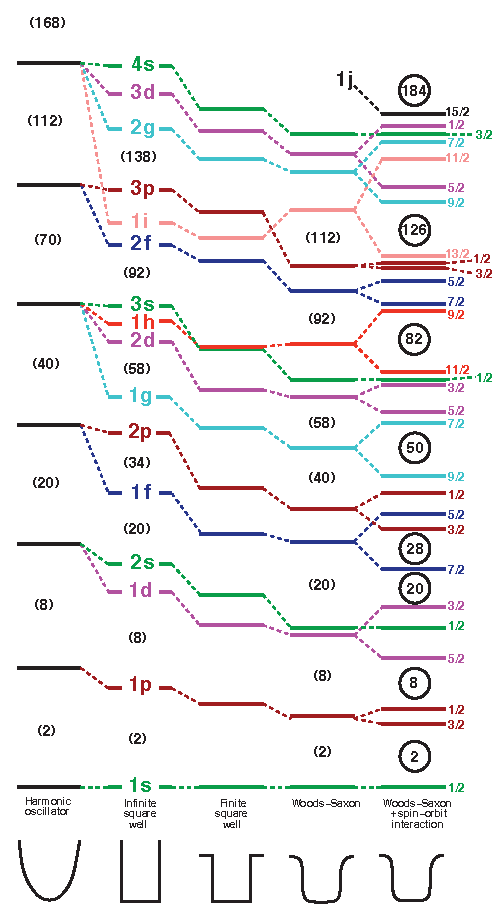
\includegraphics[width=\columnwidth,height=0.9\textheight,keepaspectratio]{Kay_Thesis_23}%
}
\caption[Nuclear energy levels based on different potentials leading to the magic numbers]{Nuclear energy levels based on different potentials leading to the magic numbers.  The oscillator number is given at left.  Numbers in parentheses are the magic numbers predicted using the specified potential.  The circled numbers in the right column corresponding to the Woods-Saxon potential with a spin-orbit interaction are the nuclear magic numbers close to stability.  Figure modified from Ref.~\cite{Kay_2007}.}%
\label{magic_numbers}%
\end{figure}

The shape of a potential that is between that of a harmonic oscillator and a square well is the Woods-Saxon potential
\begin{equation}
f(r,r_0,a)=\left[1+\exp \left(\frac{r-r_0}{a}\right)\right]^{-1} \qquad \textrm{Woods-Saxon}
\label{eq:woods_saxon}
\end{equation}
where $r$ is the dependent variable (the radius), $r_0=RA^{1/3}$ is the nuclear radius; $R$ has a typical value of 1.25\,fm and $a$, the diffuseness parameter, is on the order of 1\,fm. 
The fundamental shape of this potential is shown in Fig.~\ref{magic_numbers}; a function plot of this potential is given in Fig.~\ref{potentials}.  The degeneracy of each level produced by the Woods-Saxon potential and the square well, both central potentials, is $2(2\ell+1)$, where $\ell$ is the orbital angular momentum of the state.  Although the Woods-Saxon potential shifts the position of the energy levels relative to the finite square well, it still does not reproduce the magic numbers observed in experiment.

\begin{figure}%
\centering
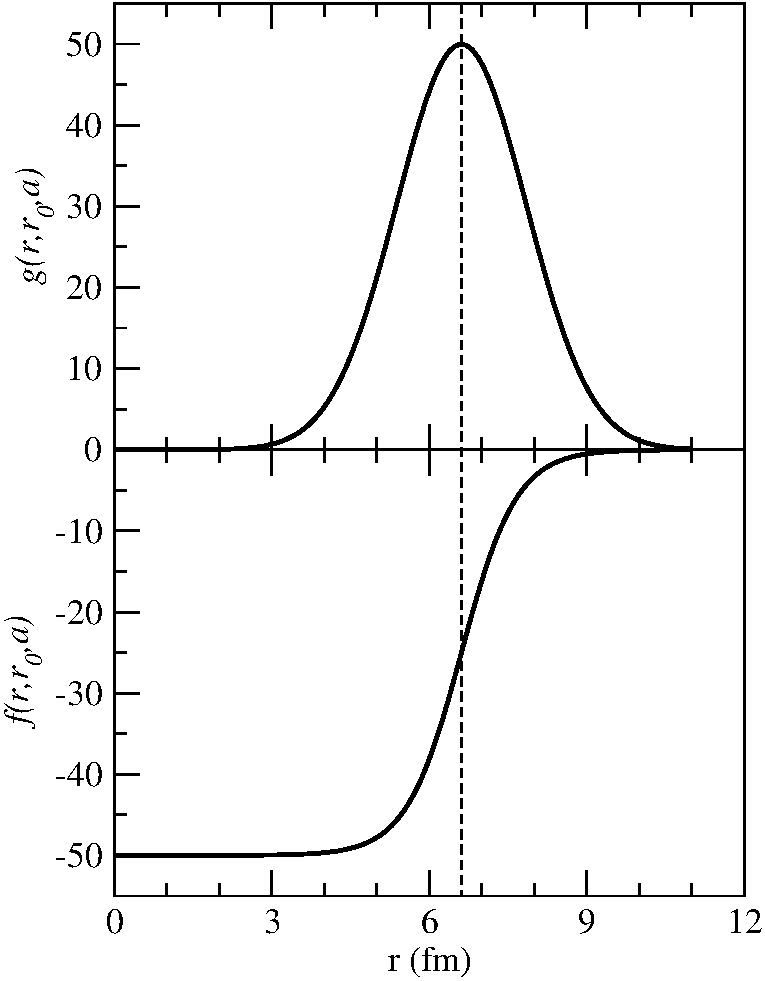
\includegraphics[width=\columnwidth,height=0.33\textheight,keepaspectratio]{potentials}%
\caption[Functional plot of the Woods-Saxon potential]{Functional plot of the Woods-Saxon potential.  The volume potential $f(r)$ (Eq.~\ref{eq:woods_saxon}) and the surface-derivative potential $g(r)$ (Eq.~\ref{eq:surface}) are plotted.  The depth of the well has been selected to be 50\,MeV.  The dashed line indicates the nuclear radius $R=6.6$\,fm, corresponding to an $A=28$ nucleus.}%
\label{potentials}%
\end{figure}

The breakthrough of Goeppert-Mayer and Jensen \textit{et al.} is the inclusion of the non-central nuclear spin-orbit potential.  %At the time, 
The idea of spin-orbit coupling was already well-known in chemistry, arising from the electromagnetic interaction between a nucleus and an orbiting electron.
  The general form of the nuclear spin-orbit potential is the same as the atomic spin-orbit potential.  However, empirically, the nuclear spin-orbit potential arises from the nucleon-nucleon interaction is of opposite sign and 20--30 times stronger than atomic spin orbit potential~\cite{Krane_1988,Satchler_1990}.  The nuclear potential is then rewritten as 
\begin{equation}
U(r)=-V f(r,R,a)+V_\mathrm{SO} \frac{1}{r} \frac{d}{dr} f(r,R,a) (\vec{\ell}\cdot\vec{s}) 
\qquad \textrm{Thomas form}
\label{eq:optical}
\end{equation}
where $V$ and $V_\mathrm{SO}$ are the depth of the volume and surface-peaked potentials, respectively. 
 The depth of the volume potential $V$ is typically on the order of 50\,MeV.  With this new potential, each level with $\ell>0$ is split into two new levels.  For a given value of $\ell$, the $j=\ell+\frac{1}{2}$ state has lower energy, and the $j=\ell-\frac{1}{2}$ state has higher energy.  The energy difference is proportional to $\frac{1}{2}(2\ell+1)\hbar^2$.  Starting with the $n=3$ oscillator shell (2$p$1$f$), the highest angular momentum state is pushed down to energies comparable to the preceding oscillator shell (see Fig.~\ref{magic_numbers}). This is the interaction which correctly reproduces the observed magic numbers 28--126.

The stable nuclei with closed proton and neutron shells, such as $^{40}$Ca and $^{208}$Pb, have been well understood within the context of the shell model for decades.  However, only recently has it been possible to study experimentally  exotic nuclei around the neutron-rich double shell closure of $Z=50$, $N=82$.  As such, the doubly-magic $^{132}$Sn nucleus is the subject of increasing attention in the nuclear physics community.  With the development of the Helical Orbit Spectrometer (HELIOS) and the Californium Rare Isotope Breeder Upgrade (CARIBU) at the ATLAS facility of Argonne National Laboratory, ground-breaking measurement opportunities are on the horizon.

\section{The Stellar \textit{r}-process}
\label{astro}
\subsection{Background}
In 1957, the seminal work ``Synthesis of the Elements in Stars'' by Burbidge, Burbidge, Fowler, and Hoyle laid the foundation of understanding nucleosynthesis in the universe~\cite{Burbidge_1957}.  An important process in stellar nucleosynthesis is the rapid neutron capture process ($r$-process), which accounts for synthesis of about half of the chemical elements with atomic mass greater than $A=50$~\cite{Martinez-Pinedo_1999}.  
Nuclei involved in the stellar $r$-process are therefore of key importance in understanding the isotropic abundances found in the universe.  The $r$-process occurs in environments of extreme neutron flux, where free neutron density is on the order of $n_n\geq10^{21}$\,cm$^{-3}$, and temperatures in the $T\geq1$\,GK range~\cite{Iliadis_2007}.  

Based on these extreme environmental parameters, a number of exotic sites of the $r$-\-pro\-cess have been suggested~\cite{Surman_2009}, however a likely candidate is the stellar atmosphere during a core-collapse supernova, leading to the creation of a neutron star.  In such an environment, nuclei capture an increasing number of neutrons creating more and more neutron-rich isotopes.  When the environmental temperatures decrease, reducing the rate of neutron capture, $\beta$-decay becomes dominant.  The neutron-rich isotopes typically $\beta$-decay along a path of constant $A$ back towards stability. The transition from the neutron capture  regime to the $\beta$-decay regime is called \textit{freeze-out}.

One of the major influencing factors that dictates the path of the $r$-process is the competition between neutron capture ($n$,$\gamma$) and photodisintegration ($\gamma$,$n$).  As a nucleus captures successive neutrons, each added neutron has a lower binding energy.  This process continues until the neutron capture rate $\lambda_n$ is balanced by the photodisintegration rate $\lambda_\gamma$.  When the two reactions are in thermal equilibrium, $(n,\gamma)\leftrightharpoons(\gamma,n)$, and can be described by Maxwell-Boltzmann statistics, the isotopic abundance is determined by the Saha equation%, shown in Eq.~\ref{eq:saha}. 

\begin{equation}
\begin{split}
\frac{n(Z,A+1)}{n(Z,A)}&=n_n \left(\frac{2\pi \hbar^2}{m_nkT}\right)^{3/2} \frac{(2j_{Z,A+1}+1)}{(2j_{Z,A}+1)(2j_n+1)}\frac{G^\mathrm{norm}_{Z,A+1}}{G^\mathrm{norm}_{Z,A}}e^{Q_{n\gamma}/kT} \qquad \textrm{Saha equation}\\
& \propto n_n \left(\frac{2\pi \hbar^2}{m_nkT}\right)^{3/2} e^{Q_{n\gamma}/kT}\\
\end{split}
\label{eq:saha}
\end{equation}
where $n(Z,A)$ is the number density (abundance) of the nuclide $^A_ZX$, $k$ is the Boltzmann constant, $j_i$ and $G^\mathrm{norm}_{i}$ are the spins and normalized partition functions of the individual particles, respectively; and $Q_{n\gamma}$ is the neutron capture $Q$-value, or equivalently, the neutron separation energy $S_n$ of $^{A+1}_{~~~~Z}X$.
The second line of the equation is a simplification to illustrate that the abundance of adjacent isotopes depends largely on the neutron density $n_n$, the temperature $T$, and the ($n$,$\gamma$) neutron capture $Q$-value.
When the reaction rates are in equilibrium, in order for the rapid neutron capture to continue, the nucleus must undergo negative $\beta$-decay.  It is said during this time that the $r$-process is ``waiting'' for the $\beta$ decay; this assumption is called the \textit{waiting-point approximation}.

Nuclei along the $r$-process path with longer $\beta$-decay half-lives have a substantial effect on the $r$-process.  While the isotopic abundance is governed by the neutron capture $Q$-value, the elemental abundance is inversely proportional to the total $\beta$-decay rate of the isotopic chain (\textit{steady flow approximation})~\cite{Iliadis_2007}. In particular, the relatively more-stable nuclei with magic neutron numbers cause a pause in the $r$-process.  This pause leads to a greater abundance of these nuclide during the 
$r$-process, corresponding to greater solar abundance in the same mass region after $r$-process freeze-out.
These so-called ``waiting-point'' nuclei at $N=50$, 82, and 126 correspond to the three predominant peaks in the isotropic abundance spectrum shown in Fig.~\ref{abun} said to be produced by the $r$-process~\cite{Kratz_1993}.   The effect of these waiting points is so substantial that the time it takes for a seed nucleus to travel the $r$-process path is largely determined by the sum of the half-lives of nuclei near closed neutron shells~\cite{Martinez-Pinedo_1999}.  As a result, it is clear that knowledge of the shell gaps of exotic isotopes in the region of the magic numbers is essential to understanding stellar processes.  Specifically, energy levels of isotopes near the doubly-magic $^{132}$Sn shell closure are vital to understanding the synthesis of isotopes in the $A=130$ region (see Fig.~\ref{abun}).

\begin{figure}%
\centering
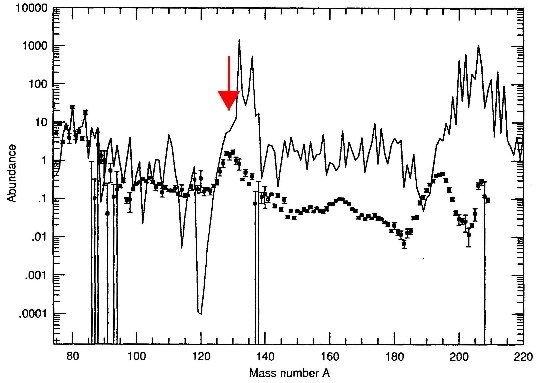
\includegraphics[width=\columnwidth,height=0.33\textheight,keepaspectratio]{Kratz_1993-fig62}%
\caption[Observed and calculated stellar $r$-process abundances]{Observed and calculated stellar $r$-process abundances.  The calculated isobaric abundances (curve) are based on the waiting-point and steady-flow approximations (described in the text) with $T_9=1.3$ and $n_n=10^{20}$\,cm$^{-3}$. Note peak near $A=130$ (indicated with arrow).  Annotated figure taken from Ref.~\cite[Fig.~6(a)]{Kratz_1993}.}%
\label{abun}%
\end{figure}

\subsection{Theoretical Framework}
Until recently, the only way to investigate the unstable neutron-rich nuclei of the $r$-process was through theoretical calculations.  The first shell-model calculations were performed in the late 1960s and early 1970 with the advent of powerful computing systems.  The following decades saw the development of advanced microscopic interaction models such as Skyrme and Gogny~\cite{Caurier_2005}.  As the development of facilities for radioactive beams drew nearer in the early 1990s, the shell properties of heavy neutron-rich isotopes gained renewed interest.  Many theorists sought to extrapolate models that described $\beta$-stable nuclei to exotic nuclei along the $r$-process path~\cite{Sharma_2002}.  An illustrative example is the comparison of predictions of mass models.  While the models tend to agree in the regions with experimental data, they diverge wildly when extrapolated to exotic nuclei as shown in Fig.~\ref{quench}~\cite{Dillmann_2003}.

\begin{figure}%
\centering
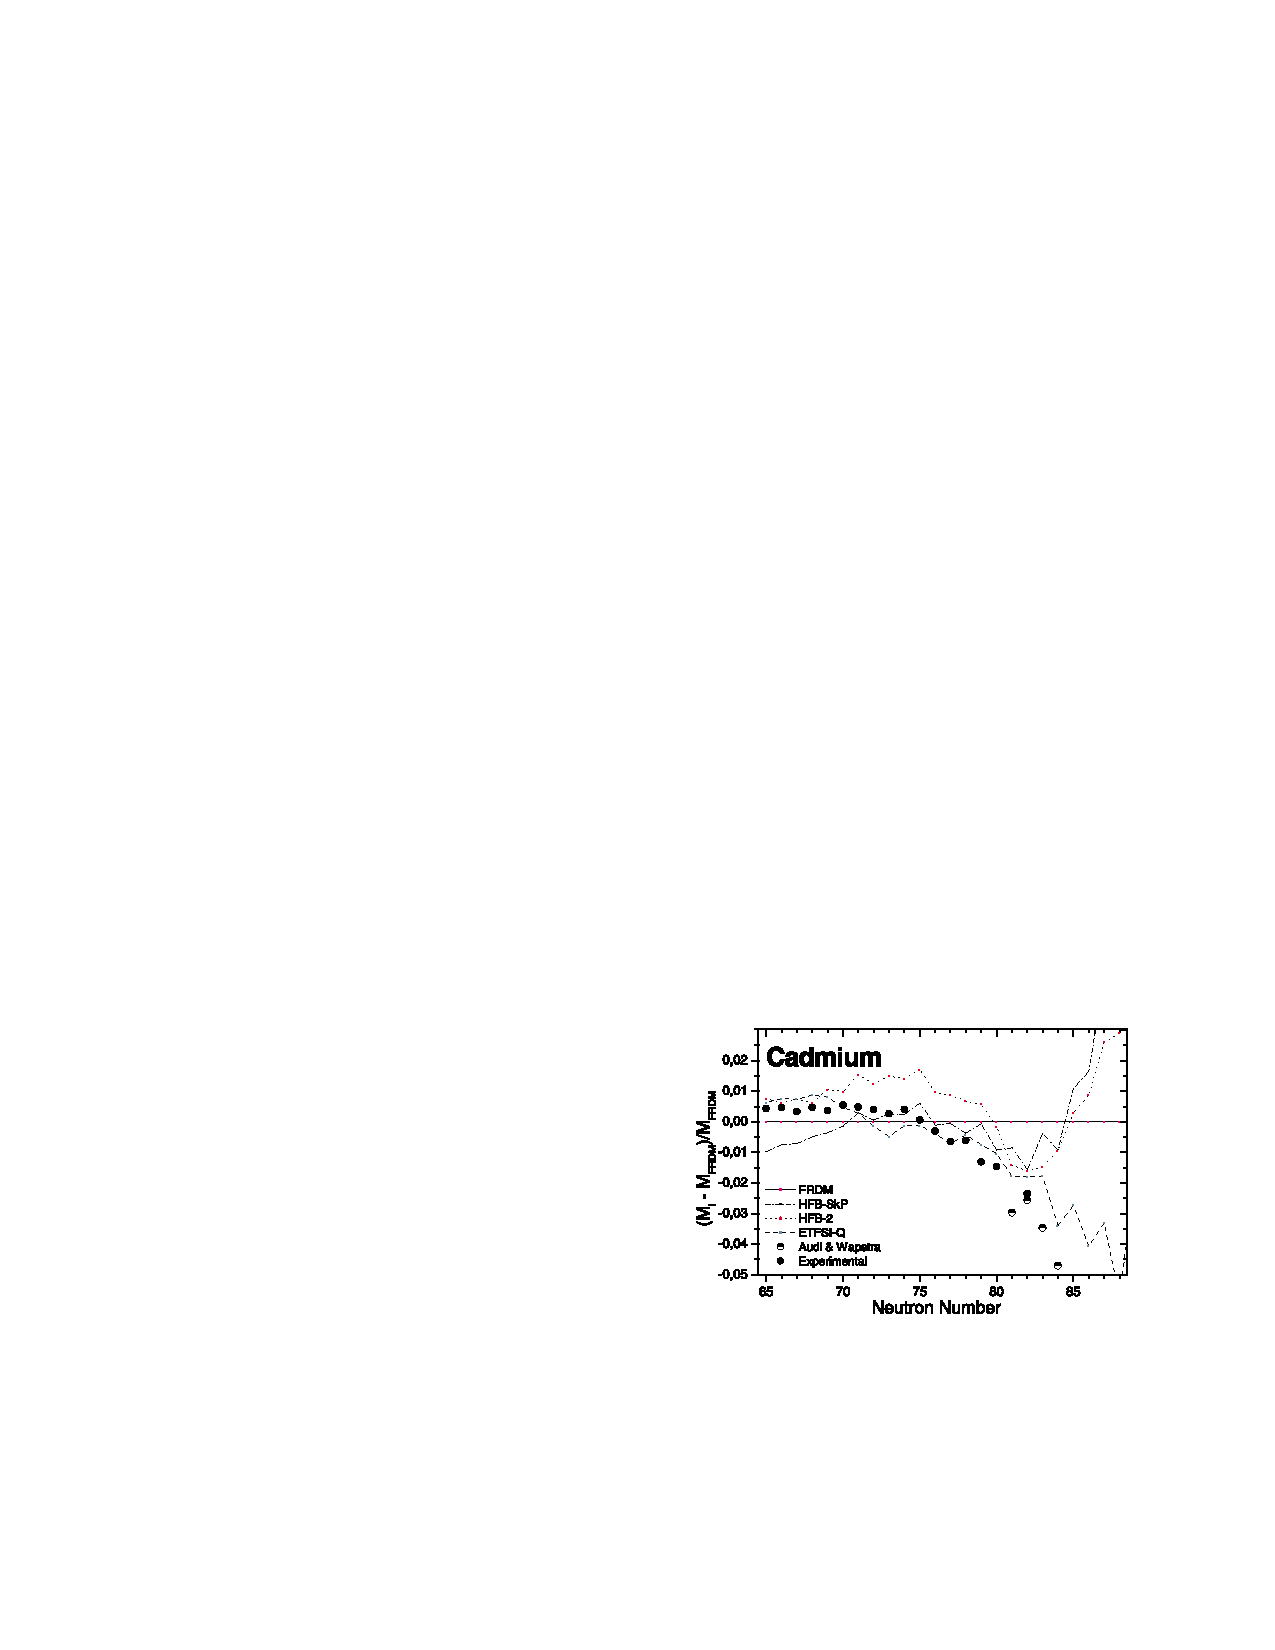
\includegraphics[width=0.75\columnwidth,keepaspectratio]{Dillmann_2003-fig3}%
\caption[Illustration of shell quenching in the Cd isotopes ($Z=48$)]{Illustration of shell quenching in the Cd isotopes ($Z=48$).  Measured isotope masses (full circles), short-range mass extrapolations (half-circles) and calculated masses (lines) are plotted relative to the finite-range liquid droplet model (FRDM).  Mass trends below the FRDM line are a signature of shell quenching.  Figure from Ref.~\cite[Fig.~3]{Dillmann_2003}}%
\label{quench}%
\end{figure}

The lack of a shell model that globally fits experimental results thus invited theorists to apply a variety of techniques to try to predict the evolution of nuclear structure with increasing neutron excess towards  the $r$-process nuclei (and beyond to the neutron drip line).  For example, the Hartree-Fock-Bogoliubov (HFB) calculations using the Skyrme force SkP and the relativistic mean-field (RMF) approximation both show significantly different predictions for properties of exotic nuclei than for $\beta$-stable nuclei.  While both models showed similar increased diffuseness in the neutron potential, they disagreed dramatically in their predictions of the spin-orbit splitting~\cite{Dobaczewski_1994}.

As discussed in \S\,\ref{sec:shell}, the effect of spin-orbit splitting is a fundamental factor influencing the formation of magic number shell gaps.   More specifically, it is the presence of a non-central spin-orbit term in the nuclear potential that produces the shell gaps in the naive shell model~\cite{Krane_1988}.   This effect is shown in the rightmost column of Fig.~\ref{magic_numbers}.  As shown in Eq.~\ref{eq:optical}, the spin-orbit potential, and thus the spin-orbit splitting, is proportional to the gradient of the nuclear potential~\cite{Grawe_2005}.  The diffuse nuclear surface and larger spacial extent of neutron-rich nuclei can produce a softening of the nuclear potential.  The resultant weakening of the spin-orbit potential reduces, or otherwise alters, the shell gaps~\cite{Schiffer_2004}.

Another important aspect of shell spacing is the effect of the tensor force, the effect of which is \textit{not} shown in Fig.~\ref{magic_numbers}.  The tensor component of the nuclear potential connects the $^3S_1$ ($L=0$) angular momentum state and the $^3D_1$-state ($L=2$) in the deuteron to produce the measured magnetic dipole and electric quadrupole moments~\cite{Wong_1998}.  In a similar fashion, the tensor force connects single-particle orbitals above closed nuclear shells.  The interaction between adjacent levels can be either attractive (deuteron-like) or repulsive and is responsible for trends in spacing of single particle levels~\cite{Otsuka_2005}.% (see Fig.~3).\marnote{figure referenced}

If the shell gaps diminish or are not present, the shell effects are said to be ``quenched.''  This was an early prediction of the HFB method and suggested that the $N=82$ shell closure may be quenched along the $r$-process path.   However, without making any assumptions about shell quenching in the model, the SkP force used in the HFB calculations intrinsically predicts smaller shell gaps than in other models~\cite{Sharma_2002}.  Furthermore, when applied to shell gaps for which experimental data exists, not only does SkP underestimate the shell gaps, it does not fit the data as well as other calculations, such as relativistic Hartree-Bogoliubov (RHB) model. 

That is not to say that shell quenching does not happen.  Any reasonable force model shows decreasing shell gaps, \textit{i.e.}, lower  as nuclei become more neutron-rich.  This reduction of the shell gaps is due to the decreasing neutron separation energy as more neutrons are added to the nucleus, which is a key feature of the $r$-process.  As the binding energy of each additional neutron becomes smaller and smaller, the shell gap eventually disappears.  With enough neutron excess, all of the shell gaps quench at the \textit{terminus stratum} of the neutron drip line.

\subsection{Initial Measurements}
In the absence of further experimental data, it would remain an open question where shell quenching occurred among the $N=82$ isotones and to what extent the effect was present in $^{132}$Sn.  In the meantime, the predictions from models explicitly involving shell quenching and experimental data from a suite of $\beta$-decay studies performed at the ISOLDE facility at CERN would seem to support a reduction of the shell gap above $N=82$.  The experimental evidence offered by the first of these studies was inconclusive due to isobaric contamination but suggested a relatively small $E$(2$^+$) value of 957\,keV for $^{130}$Cd~\cite{Kautzsch_2000}.  The follow-up study utilized significantly more advanced background suppression, but showed inconsistent results for cadmium and tin~\cite{Dillmann_2003}.  These studies emphasized the difficulties of these measurements and the need for further measurements while leaving the $N=82$ shell gap on uncertain ground.

More recently, two experiments have brought about a ``restoration'' of the $N=82$ shell gap in $^{132}$Sn.  The first was a study done at GSI that measured $\gamma$-ray transitions in $^{130}$Cd, which at the time of publication was the most neutron-rich $N=82$ isotope with observed  $\gamma$-ray transitions~\cite{Jungclaus_2007}.  The $^{130}$Cd isomers were produced in a knockout reaction and in a beam-fragmentation reaction.  What made this study unique is that it measured $\gamma$-ray transitions in coincidence with ions unambiguously identified using a fragment separator.  By measuring the transitions in coincidence with explicit ion identification, it was clear the $\gamma$-rays were being produced in isomeric decay of the isotone of interest.  The study measured a larger $E$(2$^+$) value than found in previous studies, strengthening the argument for the $N=82$ shell gap.  

Further reinforcement came from another experiment performed at CERN with ISOLDE.  This most recent study was a mass measurement using the ISOLTRAP Penning trap mass spectrometer~\cite{Dworschak_2008}.  In order to circumvent problems with isobaric contamination, the $^{132}$Sn was made into a sulfide and the resultant $^{132}$Sn$^{34}$S$^+$ was then separated and analyzed.  The subsequent mass measurement differed from the previously accepted value for $^{132}$Sn by 480\,keV.  This new mass value also increases the accepted value of the two-neutron separation energy $S_{2n}$ for $^{132}$Sn, giving it the largest shell gap of the $N=82$ isotones (see Fig.~\ref{50_gap}).

\begin{figure}%
\centering
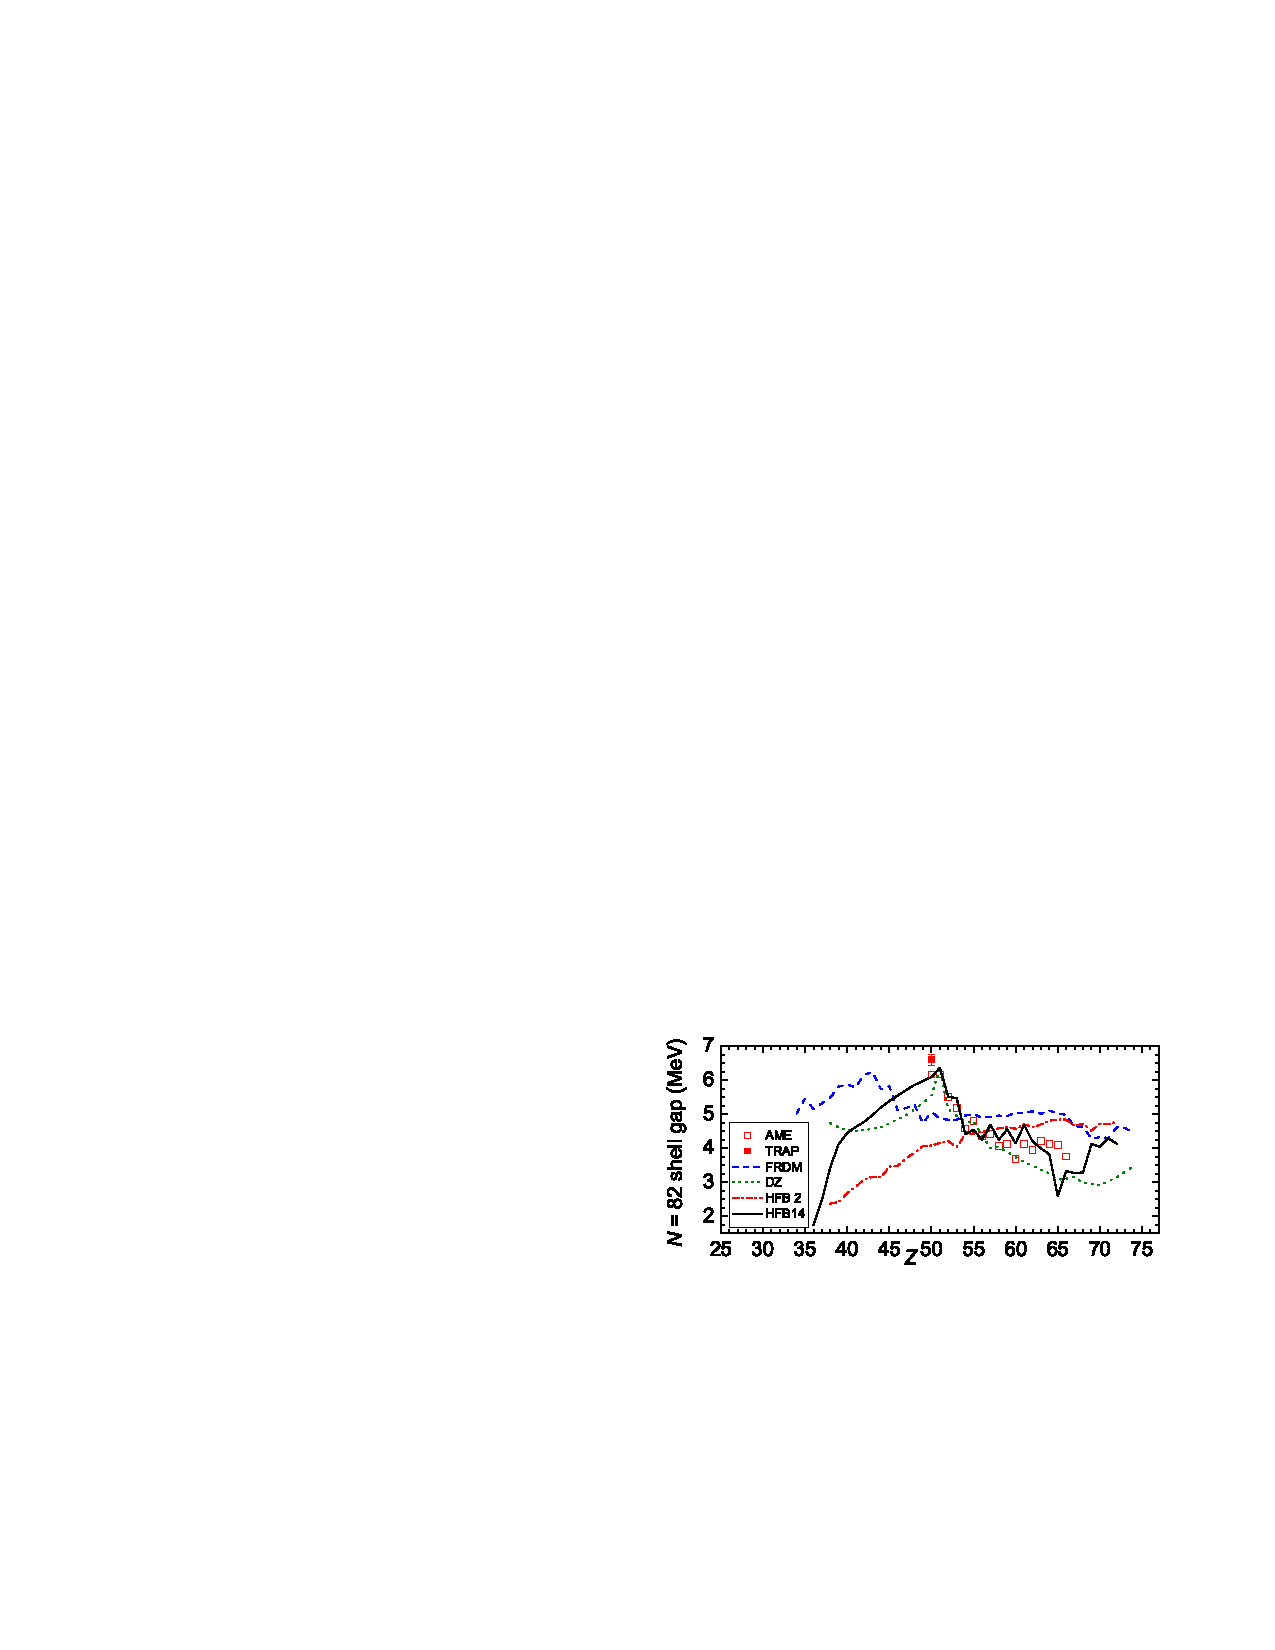
\includegraphics[width=0.75\columnwidth,keepaspectratio]{Dworschak_2008-fig3}%
\caption[Plot of the $N=82$ shell gaps as a function of $Z$]{Plot of the $N=82$ shell gaps as a function of $Z$.  The shell gaps are defined by the $S_{2n}$ energy and are determined experimentally from mass measurements.  Also plotted are a number of theoretical calculations.  The mass measurements show a peak at $Z=50$, corresponding to the doubly-magic nucleus $^{132}$Sn, meaning that the $N=82$ shell is not quenched in the tin isotopes.  Figure from Ref.~\cite[Fig.~3]{Dworschak_2008}.}%
\label{50_gap}%
\end{figure}

\subsection{Outlook}
In order to further the understanding of the $r$-process and the evolution of nuclear structure towards the neutron drip line, additional experimental data are required.  Even though $^{132}$Sn may appear to be less ``exotic'' than previously believed, its role as a doubly-magic nucleus along the $r$-process path cannot be overlooked or understated.  Information about the single-neutron states above the $^{132}$Sn shell closure will be vital to forming a complete picture of nuclear structure in this region.

At present, the majority of published experimental data related to energy levels of nuclei in the vicinity of $^{132}$Sn come from $\beta$-decay studies.  The first study of the single-neutron states in $^{132}$Sn was performed at ISOLDE~\cite{Hoff_1996}.  Indium isotopes were produced in by beam-induced fission of uranium and the subsequent $\beta$-decays were studied.  By measuring $\gamma$-rays in coincidence with the $\beta$-decays, the energy levels of the resultant $^{133}$Sn isomers were deduced.  Of the three energy levels proposed in this study, one has since been confirmed by measuring the prompt $\beta$-decay spectra following the spontaneous fission of $^{248}$Cm~\cite{Urban_1999}.  By gating on known isomeric transitions in $^{112}$Pd, a fission partner of $^{133}$Sn, the 1561\,keV transition, corresponding to the $h_{9/2}$ neutron level, has been confirmed.

Spins and parities can be tentatively assigned using $\beta$-decay selection rules and comparison to theoretical models, but no conclusive assignments can be made.  An additional problem with the $\beta$-decay studies in the $^{132}$Sn region is that they generally populate high-energy excited states~\cite{Hoff_1996}. The neutron separation energy of $^{133}$Sn is only 2.45\,MeV, so the higher energy states preferentially populated by $\beta$-decay are unbound against neutron emission, making them difficult to detect.   In order to effectively study the structure of low lying states it is necessary to use another method of measurement.  Direct nuclear reactions involving nucleon transfer provide a unique window to measure these quantities.  The $^{132}$Sn($d$,$p$) measurement performed by \citet{Jones_2010} is an example of such a reaction study; this measurement is discussed in Chapt.~\ref{standards}.%Introduction
%\section{The Stellar \textit{r}-process}
\label{astro}
\subsection{Background}
In 1957, the seminal work ``Synthesis of the Elements in Stars'' by Burbidge, Burbidge, Fowler, and Hoyle laid the foundation of understanding nucleosynthesis in the universe~\cite{Burbidge_1957}.  An important process in stellar nucleosynthesis is the rapid neutron capture process ($r$-process), which accounts for synthesis of about half of the chemical elements with atomic mass greater than $A=50$~\cite{Martinez-Pinedo_1999}.  
Nuclei involved in the stellar $r$-process are therefore of key importance in understanding the isotropic abundances found in the universe.  The $r$-process occurs in environments of extreme neutron flux, where free neutron density is on the order of $n_n\geq10^{21}$\,cm$^{-3}$, and temperatures in the $T\geq1$\,GK range~\cite{Iliadis_2007}.  

Based on these extreme environmental parameters, a number of exotic sites of the $r$-\-pro\-cess have been suggested~\cite{Surman_2009}, however a likely candidate is the stellar atmosphere during a core-collapse supernova, leading to the creation of a neutron star.  In such an environment, nuclei capture an increasing number of neutrons creating more and more neutron-rich isotopes.  When the environmental temperatures decrease, reducing the rate of neutron capture, $\beta$-decay becomes dominant.  The neutron-rich isotopes typically $\beta$-decay along a path of constant $A$ back towards stability. The transition from the neutron capture  regime to the $\beta$-decay regime is called \textit{freeze-out}.

One of the major influencing factors that dictates the path of the $r$-process is the competition between neutron capture ($n$,$\gamma$) and photodisintegration ($\gamma$,$n$).  As a nucleus captures successive neutrons, each added neutron has a lower binding energy.  This process continues until the neutron capture rate $\lambda_n$ is balanced by the photodisintegration rate $\lambda_\gamma$.  When the two reactions are in thermal equilibrium, $(n,\gamma)\leftrightharpoons(\gamma,n)$, and can be described by Maxwell-Boltzmann statistics, the isotopic abundance is determined by the Saha equation%, shown in Eq.~\ref{eq:saha}. 

\begin{equation}
\begin{split}
\frac{n(Z,A+1)}{n(Z,A)}&=n_n \left(\frac{2\pi \hbar^2}{m_nkT}\right)^{3/2} \frac{(2j_{Z,A+1}+1)}{(2j_{Z,A}+1)(2j_n+1)}\frac{G^\mathrm{norm}_{Z,A+1}}{G^\mathrm{norm}_{Z,A}}e^{Q_{n\gamma}/kT} \qquad \textrm{Saha equation}\\
& \propto n_n \left(\frac{2\pi \hbar^2}{m_nkT}\right)^{3/2} e^{Q_{n\gamma}/kT}\\
\end{split}
\label{eq:saha}
\end{equation}
where $n(Z,A)$ is the number density (abundance) of the nuclide $^A_ZX$, $k$ is the Boltzmann constant, $j_i$ and $G^\mathrm{norm}_{i}$ are the spins and normalized partition functions of the individual particles, respectively; and $Q_{n\gamma}$ is the neutron capture $Q$-value, or equivalently, the neutron separation energy $S_n$ of $^{A+1}_{~~~~Z}X$.
The second line of the equation is a simplification to illustrate that the abundance of adjacent isotopes depends largely on the neutron density $n_n$, the temperature $T$, and the ($n$,$\gamma$) neutron capture $Q$-value.
When the reaction rates are in equilibrium, in order for the rapid neutron capture to continue, the nucleus must undergo negative $\beta$-decay.  It is said during this time that the $r$-process is ``waiting'' for the $\beta$ decay; this assumption is called the \textit{waiting-point approximation}.

Nuclei along the $r$-process path with longer $\beta$-decay half-lives have a substantial effect on the $r$-process.  While the isotopic abundance is governed by the neutron capture $Q$-value, the elemental abundance is inversely proportional to the total $\beta$-decay rate of the isotopic chain (\textit{steady flow approximation})~\cite{Iliadis_2007}. In particular, the relatively more-stable nuclei with magic neutron numbers cause a pause in the $r$-process.  This pause leads to a greater abundance of these nuclide during the 
$r$-process, corresponding to greater solar abundance in the same mass region after $r$-process freeze-out.
These so-called ``waiting-point'' nuclei at $N=50$, 82, and 126 correspond to the three predominant peaks in the isotropic abundance spectrum shown in Fig.~\ref{abun} said to be produced by the $r$-process~\cite{Kratz_1993}.   The effect of these waiting points is so substantial that the time it takes for a seed nucleus to travel the $r$-process path is largely determined by the sum of the half-lives of nuclei near closed neutron shells~\cite{Martinez-Pinedo_1999}.  As a result, it is clear that knowledge of the shell gaps of exotic isotopes in the region of the magic numbers is essential to understanding stellar processes.  Specifically, energy levels of isotopes near the doubly-magic $^{132}$Sn shell closure are vital to understanding the synthesis of isotopes in the $A=130$ region (see Fig.~\ref{abun}).

\begin{figure}%
\centering
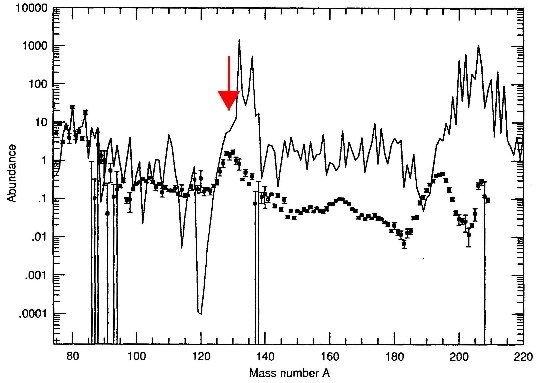
\includegraphics[width=\columnwidth,height=0.33\textheight,keepaspectratio]{Kratz_1993-fig62}%
\caption[Observed and calculated stellar $r$-process abundances]{Observed and calculated stellar $r$-process abundances.  The calculated isobaric abundances (curve) are based on the waiting-point and steady-flow approximations (described in the text) with $T_9=1.3$ and $n_n=10^{20}$\,cm$^{-3}$. Note peak near $A=130$ (indicated with arrow).  Annotated figure taken from Ref.~\cite[Fig.~6(a)]{Kratz_1993}.}%
\label{abun}%
\end{figure}

\subsection{Theoretical Framework}
Until recently, the only way to investigate the unstable neutron-rich nuclei of the $r$-process was through theoretical calculations.  The first shell-model calculations were performed in the late 1960s and early 1970 with the advent of powerful computing systems.  The following decades saw the development of advanced microscopic interaction models such as Skyrme and Gogny~\cite{Caurier_2005}.  As the development of facilities for radioactive beams drew nearer in the early 1990s, the shell properties of heavy neutron-rich isotopes gained renewed interest.  Many theorists sought to extrapolate models that described $\beta$-stable nuclei to exotic nuclei along the $r$-process path~\cite{Sharma_2002}.  An illustrative example is the comparison of predictions of mass models.  While the models tend to agree in the regions with experimental data, they diverge wildly when extrapolated to exotic nuclei as shown in Fig.~\ref{quench}~\cite{Dillmann_2003}.

\begin{figure}%
\centering
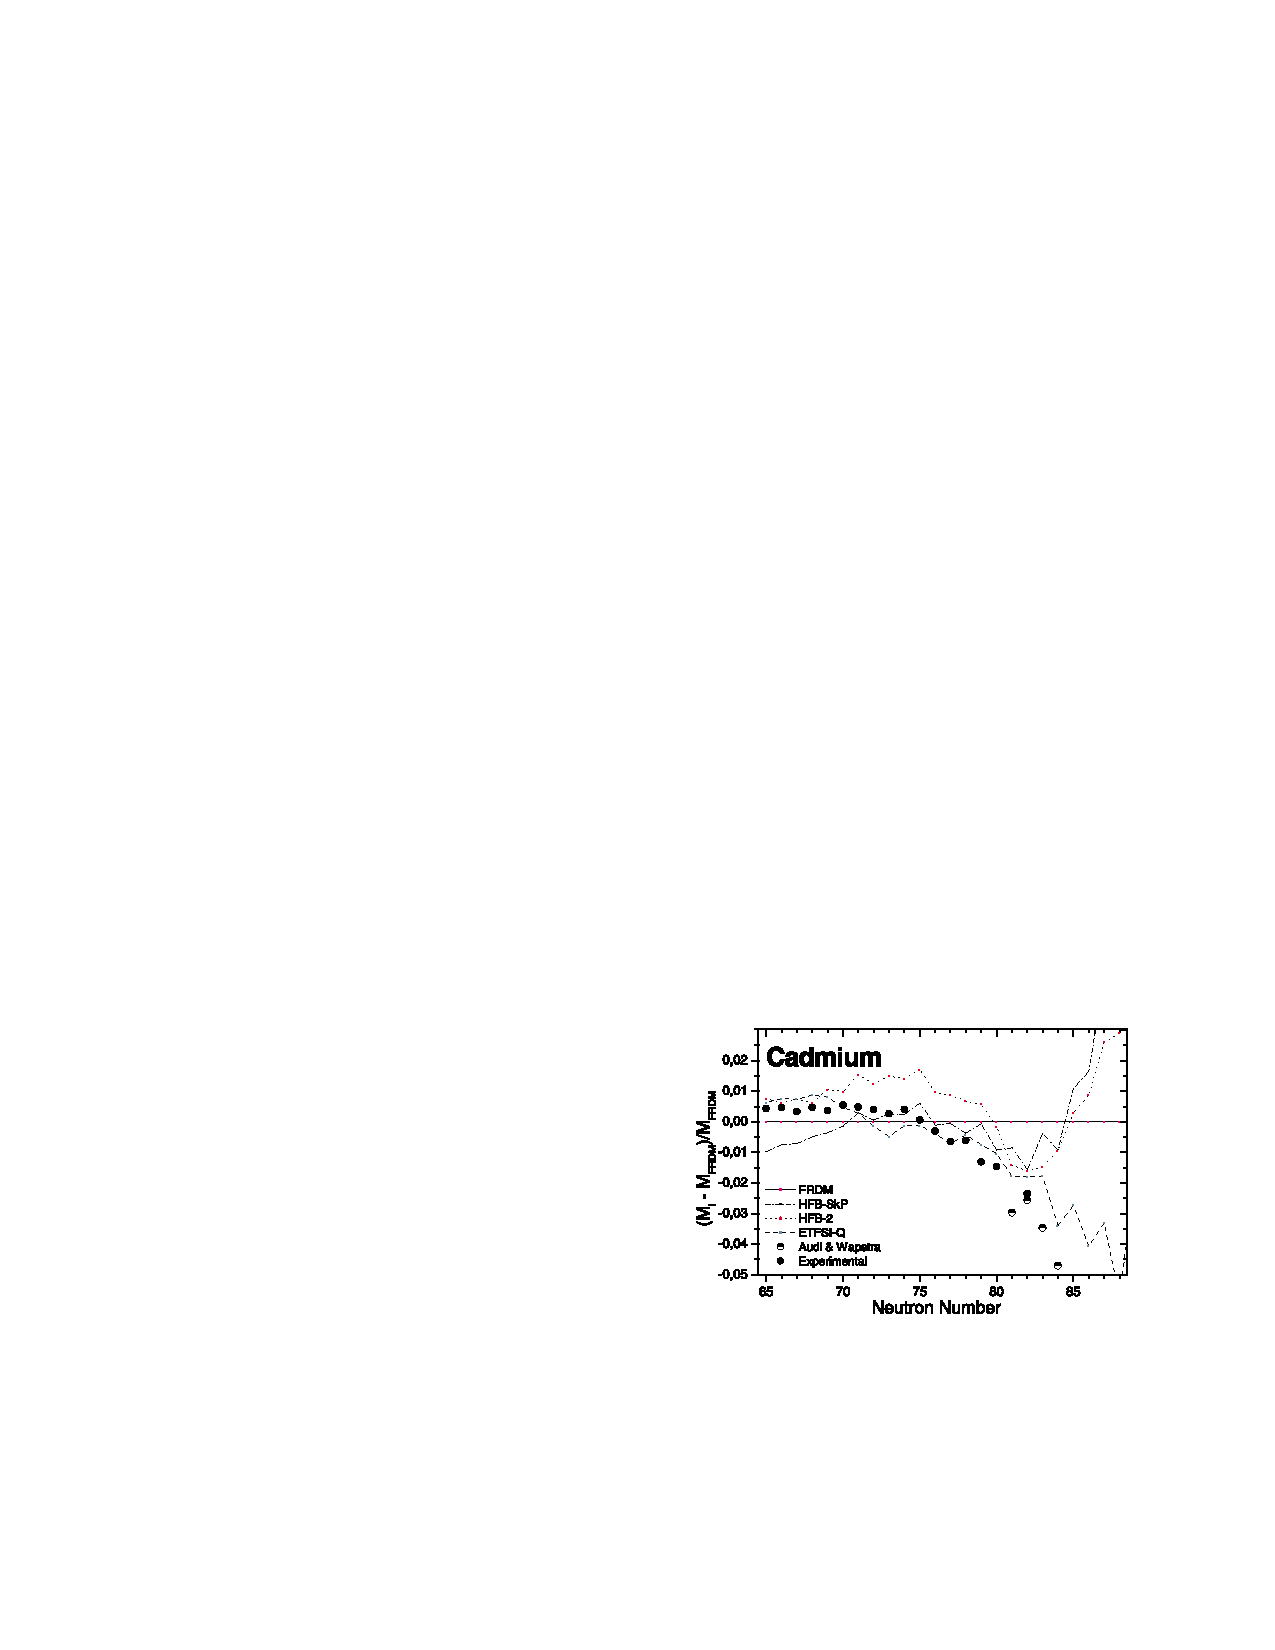
\includegraphics[width=0.75\columnwidth,keepaspectratio]{Dillmann_2003-fig3}%
\caption[Illustration of shell quenching in the Cd isotopes ($Z=48$)]{Illustration of shell quenching in the Cd isotopes ($Z=48$).  Measured isotope masses (full circles), short-range mass extrapolations (half-circles) and calculated masses (lines) are plotted relative to the finite-range liquid droplet model (FRDM).  Mass trends below the FRDM line are a signature of shell quenching.  Figure from Ref.~\cite[Fig.~3]{Dillmann_2003}}%
\label{quench}%
\end{figure}

The lack of a shell model that globally fits experimental results thus invited theorists to apply a variety of techniques to try to predict the evolution of nuclear structure with increasing neutron excess towards  the $r$-process nuclei (and beyond to the neutron drip line).  For example, the Hartree-Fock-Bogoliubov (HFB) calculations using the Skyrme force SkP and the relativistic mean-field (RMF) approximation both show significantly different predictions for properties of exotic nuclei than for $\beta$-stable nuclei.  While both models showed similar increased diffuseness in the neutron potential, they disagreed dramatically in their predictions of the spin-orbit splitting~\cite{Dobaczewski_1994}.

As discussed in \S\,\ref{sec:shell}, the effect of spin-orbit splitting is a fundamental factor influencing the formation of magic number shell gaps.   More specifically, it is the presence of a non-central spin-orbit term in the nuclear potential that produces the shell gaps in the naive shell model~\cite{Krane_1988}.   This effect is shown in the rightmost column of Fig.~\ref{magic_numbers}.  As shown in Eq.~\ref{eq:optical}, the spin-orbit potential, and thus the spin-orbit splitting, is proportional to the gradient of the nuclear potential~\cite{Grawe_2005}.  The diffuse nuclear surface and larger spacial extent of neutron-rich nuclei can produce a softening of the nuclear potential.  The resultant weakening of the spin-orbit potential reduces, or otherwise alters, the shell gaps~\cite{Schiffer_2004}.

Another important aspect of shell spacing is the effect of the tensor force, the effect of which is \textit{not} shown in Fig.~\ref{magic_numbers}.  The tensor component of the nuclear potential connects the $^3S_1$ ($L=0$) angular momentum state and the $^3D_1$-state ($L=2$) in the deuteron to produce the measured magnetic dipole and electric quadrupole moments~\cite{Wong_1998}.  In a similar fashion, the tensor force connects single-particle orbitals above closed nuclear shells.  The interaction between adjacent levels can be either attractive (deuteron-like) or repulsive and is responsible for trends in spacing of single particle levels~\cite{Otsuka_2005}.% (see Fig.~3).\marnote{figure referenced}

If the shell gaps diminish or are not present, the shell effects are said to be ``quenched.''  This was an early prediction of the HFB method and suggested that the $N=82$ shell closure may be quenched along the $r$-process path.   However, without making any assumptions about shell quenching in the model, the SkP force used in the HFB calculations intrinsically predicts smaller shell gaps than in other models~\cite{Sharma_2002}.  Furthermore, when applied to shell gaps for which experimental data exists, not only does SkP underestimate the shell gaps, it does not fit the data as well as other calculations, such as relativistic Hartree-Bogoliubov (RHB) model. 

That is not to say that shell quenching does not happen.  Any reasonable force model shows decreasing shell gaps, \textit{i.e.}, lower  as nuclei become more neutron-rich.  This reduction of the shell gaps is due to the decreasing neutron separation energy as more neutrons are added to the nucleus, which is a key feature of the $r$-process.  As the binding energy of each additional neutron becomes smaller and smaller, the shell gap eventually disappears.  With enough neutron excess, all of the shell gaps quench at the \textit{terminus stratum} of the neutron drip line.

\subsection{Initial Measurements}
In the absence of further experimental data, it would remain an open question where shell quenching occurred among the $N=82$ isotones and to what extent the effect was present in $^{132}$Sn.  In the meantime, the predictions from models explicitly involving shell quenching and experimental data from a suite of $\beta$-decay studies performed at the ISOLDE facility at CERN would seem to support a reduction of the shell gap above $N=82$.  The experimental evidence offered by the first of these studies was inconclusive due to isobaric contamination but suggested a relatively small $E$(2$^+$) value of 957\,keV for $^{130}$Cd~\cite{Kautzsch_2000}.  The follow-up study utilized significantly more advanced background suppression, but showed inconsistent results for cadmium and tin~\cite{Dillmann_2003}.  These studies emphasized the difficulties of these measurements and the need for further measurements while leaving the $N=82$ shell gap on uncertain ground.

More recently, two experiments have brought about a ``restoration'' of the $N=82$ shell gap in $^{132}$Sn.  The first was a study done at GSI that measured $\gamma$-ray transitions in $^{130}$Cd, which at the time of publication was the most neutron-rich $N=82$ isotope with observed  $\gamma$-ray transitions~\cite{Jungclaus_2007}.  The $^{130}$Cd isomers were produced in a knockout reaction and in a beam-fragmentation reaction.  What made this study unique is that it measured $\gamma$-ray transitions in coincidence with ions unambiguously identified using a fragment separator.  By measuring the transitions in coincidence with explicit ion identification, it was clear the $\gamma$-rays were being produced in isomeric decay of the isotone of interest.  The study measured a larger $E$(2$^+$) value than found in previous studies, strengthening the argument for the $N=82$ shell gap.  

Further reinforcement came from another experiment performed at CERN with ISOLDE.  This most recent study was a mass measurement using the ISOLTRAP Penning trap mass spectrometer~\cite{Dworschak_2008}.  In order to circumvent problems with isobaric contamination, the $^{132}$Sn was made into a sulfide and the resultant $^{132}$Sn$^{34}$S$^+$ was then separated and analyzed.  The subsequent mass measurement differed from the previously accepted value for $^{132}$Sn by 480\,keV.  This new mass value also increases the accepted value of the two-neutron separation energy $S_{2n}$ for $^{132}$Sn, giving it the largest shell gap of the $N=82$ isotones (see Fig.~\ref{50_gap}).

\begin{figure}%
\centering
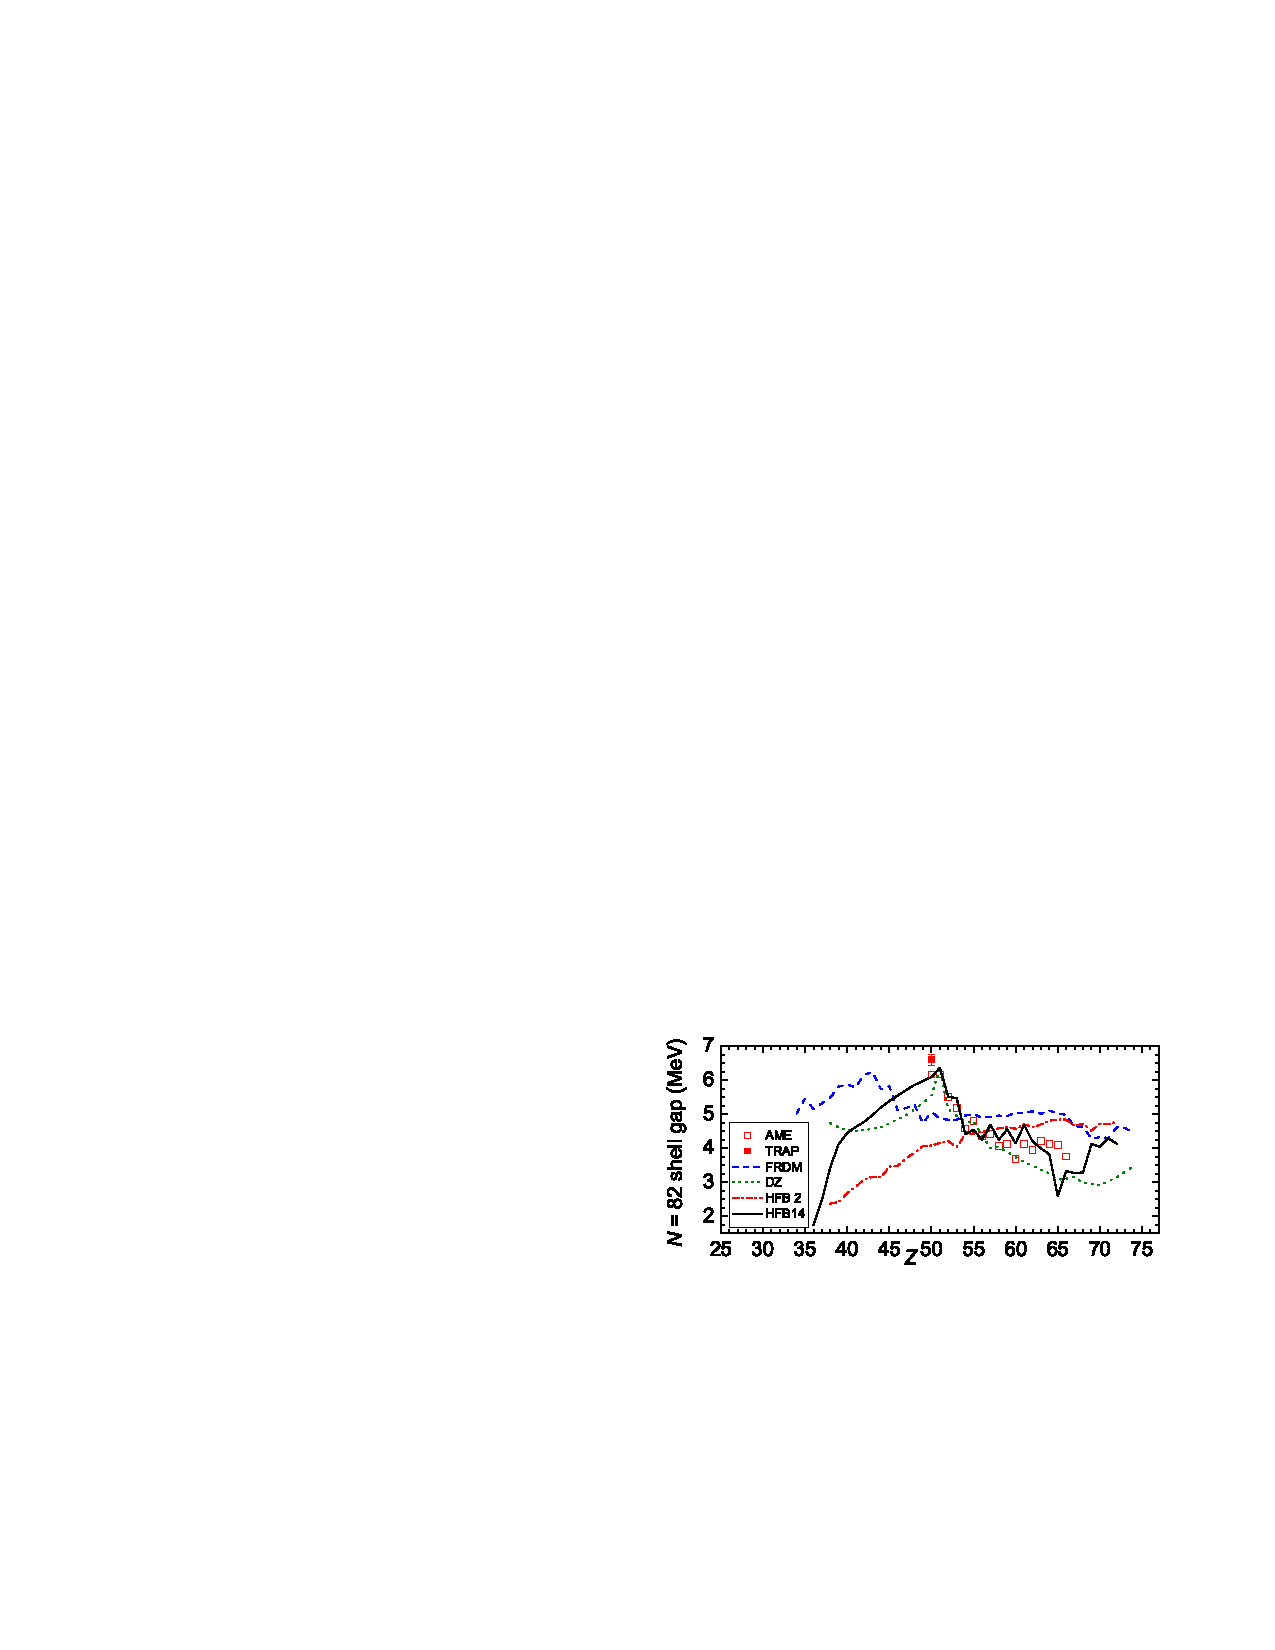
\includegraphics[width=0.75\columnwidth,keepaspectratio]{Dworschak_2008-fig3}%
\caption[Plot of the $N=82$ shell gaps as a function of $Z$]{Plot of the $N=82$ shell gaps as a function of $Z$.  The shell gaps are defined by the $S_{2n}$ energy and are determined experimentally from mass measurements.  Also plotted are a number of theoretical calculations.  The mass measurements show a peak at $Z=50$, corresponding to the doubly-magic nucleus $^{132}$Sn, meaning that the $N=82$ shell is not quenched in the tin isotopes.  Figure from Ref.~\cite[Fig.~3]{Dworschak_2008}.}%
\label{50_gap}%
\end{figure}

\subsection{Outlook}
In order to further the understanding of the $r$-process and the evolution of nuclear structure towards the neutron drip line, additional experimental data are required.  Even though $^{132}$Sn may appear to be less ``exotic'' than previously believed, its role as a doubly-magic nucleus along the $r$-process path cannot be overlooked or understated.  Information about the single-neutron states above the $^{132}$Sn shell closure will be vital to forming a complete picture of nuclear structure in this region.

At present, the majority of published experimental data related to energy levels of nuclei in the vicinity of $^{132}$Sn come from $\beta$-decay studies.  The first study of the single-neutron states in $^{132}$Sn was performed at ISOLDE~\cite{Hoff_1996}.  Indium isotopes were produced in by beam-induced fission of uranium and the subsequent $\beta$-decays were studied.  By measuring $\gamma$-rays in coincidence with the $\beta$-decays, the energy levels of the resultant $^{133}$Sn isomers were deduced.  Of the three energy levels proposed in this study, one has since been confirmed by measuring the prompt $\beta$-decay spectra following the spontaneous fission of $^{248}$Cm~\cite{Urban_1999}.  By gating on known isomeric transitions in $^{112}$Pd, a fission partner of $^{133}$Sn, the 1561\,keV transition, corresponding to the $h_{9/2}$ neutron level, has been confirmed.

Spins and parities can be tentatively assigned using $\beta$-decay selection rules and comparison to theoretical models, but no conclusive assignments can be made.  An additional problem with the $\beta$-decay studies in the $^{132}$Sn region is that they generally populate high-energy excited states~\cite{Hoff_1996}. The neutron separation energy of $^{133}$Sn is only 2.45\,MeV, so the higher energy states preferentially populated by $\beta$-decay are unbound against neutron emission, making them difficult to detect.   In order to effectively study the structure of low lying states it is necessary to use another method of measurement.  Direct nuclear reactions involving nucleon transfer provide a unique window to measure these quantities.  The $^{132}$Sn($d$,$p$) measurement performed by \citet{Jones_2010} is an example of such a reaction study; this measurement is discussed in Chapt.~\ref{standards}.
\chapter{Nuclear transfer reactions}
\label{chapt:reactions}
In terms of nuclear physics, a nuclear reaction occurs when two atomic nuclei collide and transform to produce new nuclei different from the reactants.  Use of a particle accelerator is needed in order for the colliding particles to have sufficient kinetic energy to overcome the Coulomb repulsion due to the nuclear charge.  A special class of nuclear reactions called ``transfer reactions'' involve the transfer of a small number of nucleons between the reactants during the process of the reaction.  This chapter discusses the utility of studying such nuclear reactions and how they provides a powerful analytic tool for understanding  nuclei.  Transfer reactions are one of several methods that allow the study of the position of excited states in a nucleus.  Other methods include $\beta$-decay $\gamma$-decay studies.  What makes transfer reaction studies unique is the way in which they provide information on the quantum number associated with the spin and parity of nuclear energy levels.  In addition, transfer reactions provide information on the single particle structure of a nucleus.

\section{Direct Reactions}
In the most basic form of a direct reaction, an incident beam particle has a single collision with a target nucleus, interacting with a single degree of freedom in the target nucleus.  Direct transfer reactions are characterized by short interaction time $t\sim2r_0/v_1$ where $r_0$ is the radius of the target nucleus and $v_1$ is the velocity of the incident ion.  The amount of energy transferred in these reactions is small compared to the incident beam energy; thus these reactions are sometimes referred to as being  ``quasi-elastic'' to differentiate them from deep-inelastic nuclear reactions. 

\begin{figure}%
\centering
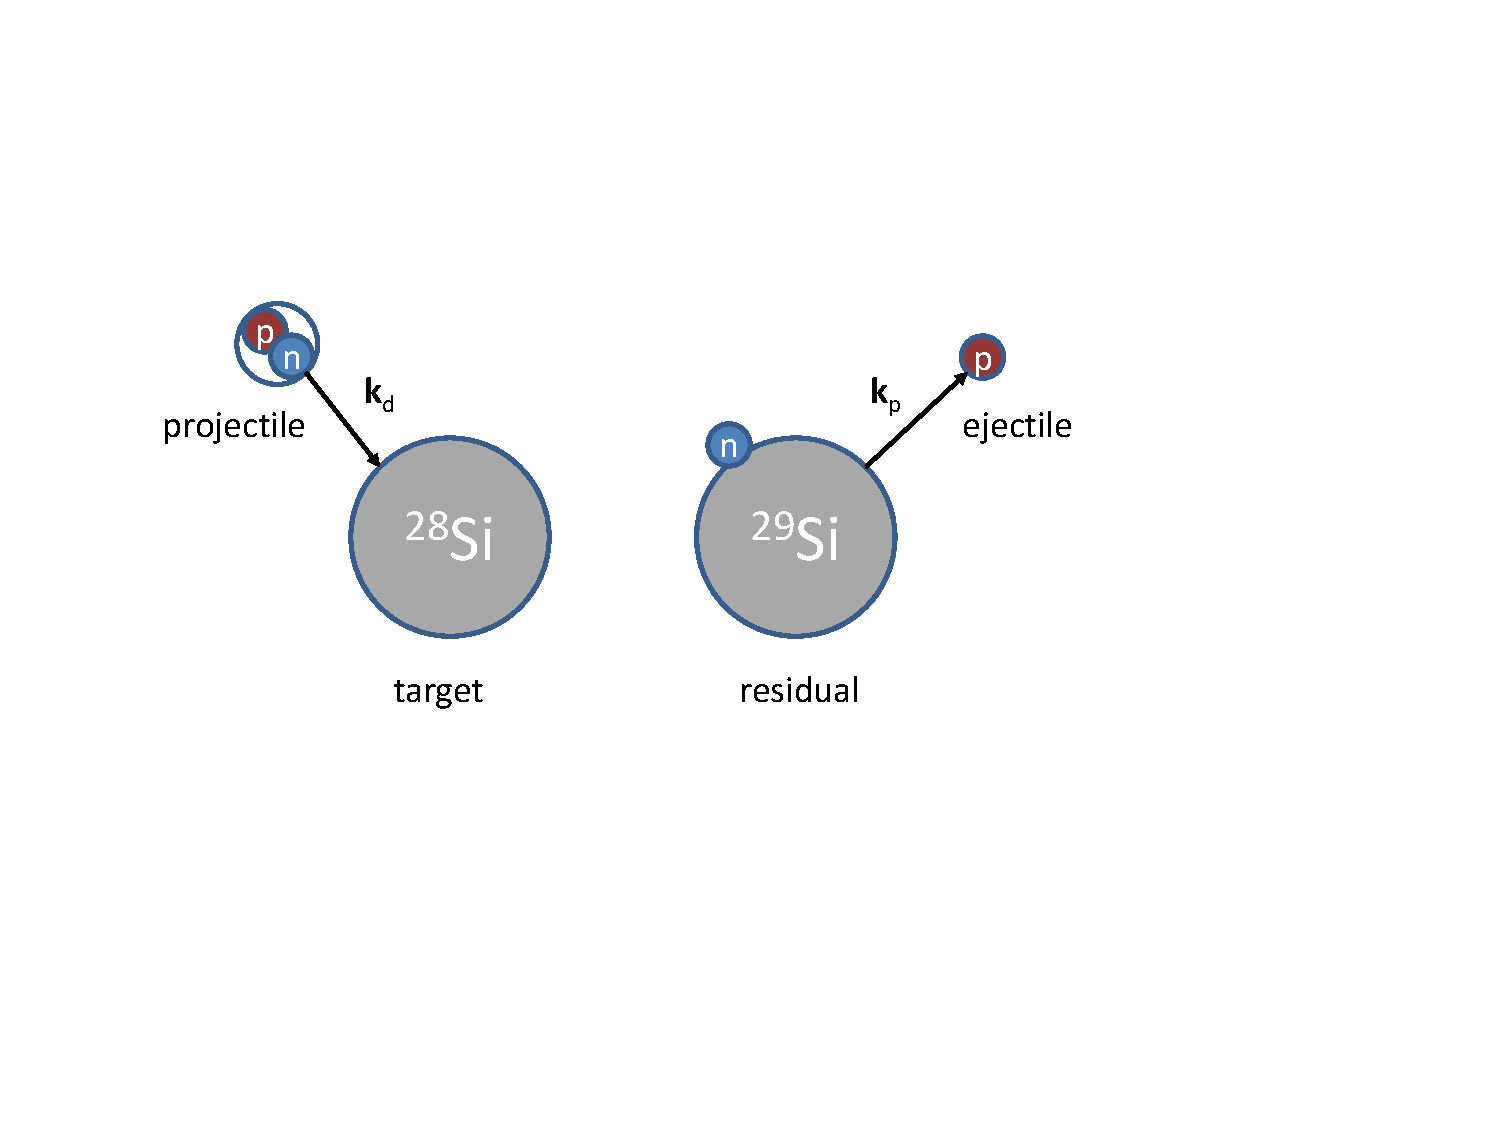
\includegraphics[width=0.75\columnwidth,height=0.33\textheight,keepaspectratio]{dp_schem2}%
\caption[Schematic illustration of the ($d$,$p$) reaction]{Schematic illustration of the ($d$,$p$) reaction.  The  deuteron has an incident momentum of $k_d$. After colliding with the $^{28}$Si target nucleus, the neutron is stripped from the beam particle and the proton has an outgoing momentum of $k_p$.}%
\label{dp_fig}%
\end{figure}

\subsection{Notation}
In the prototypical example, a stationary target is bombarded by an accelerated beam of particles and a detector measures the scattered particles.  The reaction may be written as
\begin{equation}
A+a\rightarrow B+b
\label{basic_reaction}
\end{equation}
where $A$ is the heavy ion reactant; $a$ is the light ion reactant; $B$ is the heavy ion recoil; and $b$ is the light ion recoil.  In this notation, the reaction can be written in a more compact form as $A$($a$,$b$)$B$ with ($a$,$b$) identifying the type of reaction.   

This notation convention was developed during a time with the reactions being studied typically involved a light ion beam and a heavy ``ion'' target---here the term ion is used loosely, as the target are not typically ionized.  To make consistent use of this notation, the first reactant listed is defined as the target nucleus and the second reactant is defined as the beam particle or projectile.  Therefore, under this convention, a reaction in which the heavy reactant is accelerated (``inverse kinematics'') would be written as $a$($A$,$b$)$B$, even though the reaction would still be referred to as an ``($a$,$b$)'' reaction.  Similarly, the light ion ejectile $b$ is traditionally the detected particle, or the particle of interest.  Adopting the notation, a reaction in which the heavy recoil is the particle of interest or a measurement in which the heavy ion is detected can be written as $A$($a$,$B$)$b$. 

In elastic scattering, the incoming particle $a$ and the outgoing particle $b$ are the same, leaving the ion species of the target nucleus unchanged.  In a transfer reaction,  $a$ and $b$ are different from each other.  The form of this difference divides transfer reactions into three different classes, given names from the perspective of the light ion projectile.  For example, in a ``stripping'' reaction, nucleons are stripped from the incident projectiles by the target nucleus.  Examples of stripping reactions include ($d$,$p$) and ($^3$He,$d$) which are neutron and proton stripping reactions, respectively.  These reactions add nucleons to the target nucleus.  The inverse of this process is referred to as a ``pick-up'' reaction, where the incident projectile picks-up nucleons from the target.  For example ($d$,$^3$He) and ($t$,$\alpha$) are proton pick-up reactions.

In a typical nucleon transfer reaction, a heavy target is bombarded by an accelerated beam of stable light nuclei.  A classic example of such a reaction is a deuteron beam striking a stable $^{28}$Si target to produce $^{29}$Si~\cite{Mermaz_1971}, illustrated in Fig.~\ref{dp_fig}.  In such an experiment, the ejected proton is detected in order to study the properties of $^{29}$Si.  Traditionally, the ejected light ion is detected with silicon detectors through a range of fixed laboratory angles---other detectors may also be used, such as photographic plates, gas counters, \textit{etc.}  Charge collection in the detectors determines the ejected particle's energy and the position of the detector determines the laboratory angle.  Detectors can be segmented or position-sensitive for enhanced angular resolution.
 
\subsection{Single-particle States}
What makes direct nuclear reactions unique is the wealth of information they provide and the relative ease with which they provide it.  In a traditional experiment, involving an isotopically pure beam and a target which is either isotopically pure or of a known composition, there is little question as to the source of the measured results.  In turn, this makes particle identification nearly unnecessary, eliminating the need for additional detectors and electronics.

Single particle states around closed-shell nuclei serve as a benchmark for testing nuclear structure theories.  At present, there is no global theory describing nuclear properties across the chart of the nuclides.   The properties of stable nuclei are well understood.  However, the diffuse surfaces of neutron-rich nuclei may leads to changes in the nuclear potential and this effect is not completely understood~\cite{Dobaczewski_1994,Grawe_2005}.  As a result, it is unclear how the ordering and spacing of single particle states evolve with increasing neutron excess.

One of the main goals of studying valence states around shell closures is to identify the ordering of the single-particle orbitals.  To use $^{133}$Sn as an example, past studies populating states in $^{133}$Sn   and measuring subsequent $\gamma$-ray transitions have shed some light on the energy levels above the $^{132}$Sn core~\cite{Hoff_1996,Urban_1999}.  However, the value of transition energies gained in such studies yields no direct information on the ordering of the levels or the spin and parity of the states.  The key to further progress in understanding the structure of $^{133}$Sn lies in nucleon-transfer reactions.  One of the powerful aspects of direct transfer reactions is their selectivity.  The reactions preferentially populate states that are well describe as target $+$ nucleon system.  In the $^{132}$Sn($D$,$p$) reaction, one would expect states to be populated that correspond to neutron occupying the orbits in the $2f$ $3p$ shell and the $1h_{9/2}$ orbital. 

\section{Plane-wave Theory}
Direct nuclear reactions, such as the nucleon transfer reaction ($d$,$p$),  are well suited to populate low energy, low angular momentum states. These low lying states tend to have single particle structure, particularly above closed-shell nuclei.  It is the access to these single-particle levels provided by direct nuclear reactions which make them of specific interest in understanding both nuclear structure and astrophysical processes.  It is not surprising then, that this technique has been well-established as an analytical tool for decades.  The lowest-order theory describing direct reaction describes the incoming projection and outgoing ejectile as plane waves (\textit{first Born approximation})~\cite{Glendenning_2004}.  This method was first used by \citet{Butler_1950} to describe the ($d$,$p$) reaction.%\cite{Satchler_1990}

\subsection{Momentum Transfer}
In a semi-classical description the incident plane wave will have a momentum vector $p_i=\hbar k_i$.  Due to the interaction of the projectile with the target, the change in momentum of the incident particle will be $q=k_i-k_f$.  Continuing from the assumption that the reaction occurs at the nuclear surface, the radius of the target nucleus may be written as $r_0=R A^{1/3}$ and the angular momentum transferred to the target nucleus is $\ell=r_0 \times q$. The scattering angle connecting $\ell$ and $q$ is then given by
\begin{equation}
\theta_\mathrm{}=\arccos\left(\frac{k_f^2+f_i^2-(\ell/r_0)^2}{2k_fk_i}\right).
\label{eq:theta_max}
\end{equation}

Fig.~\ref{l_matching} shows the results of semi-classical calculations for momentum-matching for various pro\-ton-\-strip\-ping reactions on $^{118}$Sn.  This naive interpretation of nuclear scattering actually provides a useful description of the reaction.  Fig.~\ref{l_matching_spectra} shows the excitation energy spectra of the same nucleus, $^{118}$Sn, populated in two different proton-stripping reactions.  The $^{118}$Sn($\alpha$,$t$)$^{119}$Sb reaction, which has a large, negative $Q$-value of -14.7\,MeV, has enhanced yield to transitions corresponding to momentum transfers of $\ell=4$ and $\ell=5$. The yield to higher-spin states populated with the $^{118}$Sn($^3$He,$d$)$^{119}$Sb reaction is reduced. 

\begin{figure}%
\centering
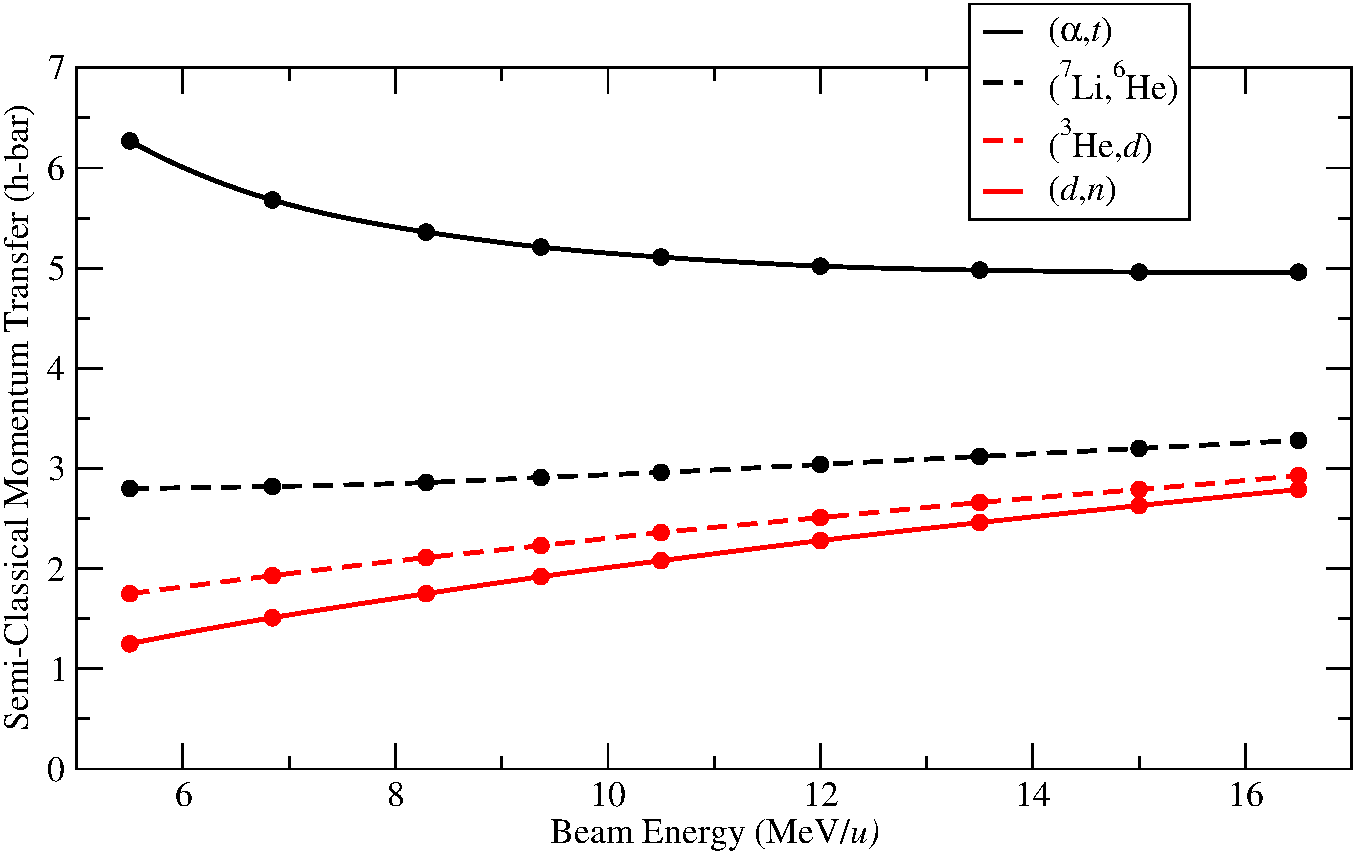
\includegraphics[width=0.9\columnwidth,height=0.4\textheight,keepaspectratio]{118Sn_l-matching}%
\caption[Semi-classical calculations of momentum-matching for proton-stripping reactions on $^{118}$Sn]{Semi-classical calculations of momentum-matching for proton-stripping reactions on $^{118}$Sn.  The calculated angular momentum transfer (in units of $\hbar$) is plotted as a function of beam energy.}%
\label{l_matching}%
\end{figure}

\begin{figure}%
\centering
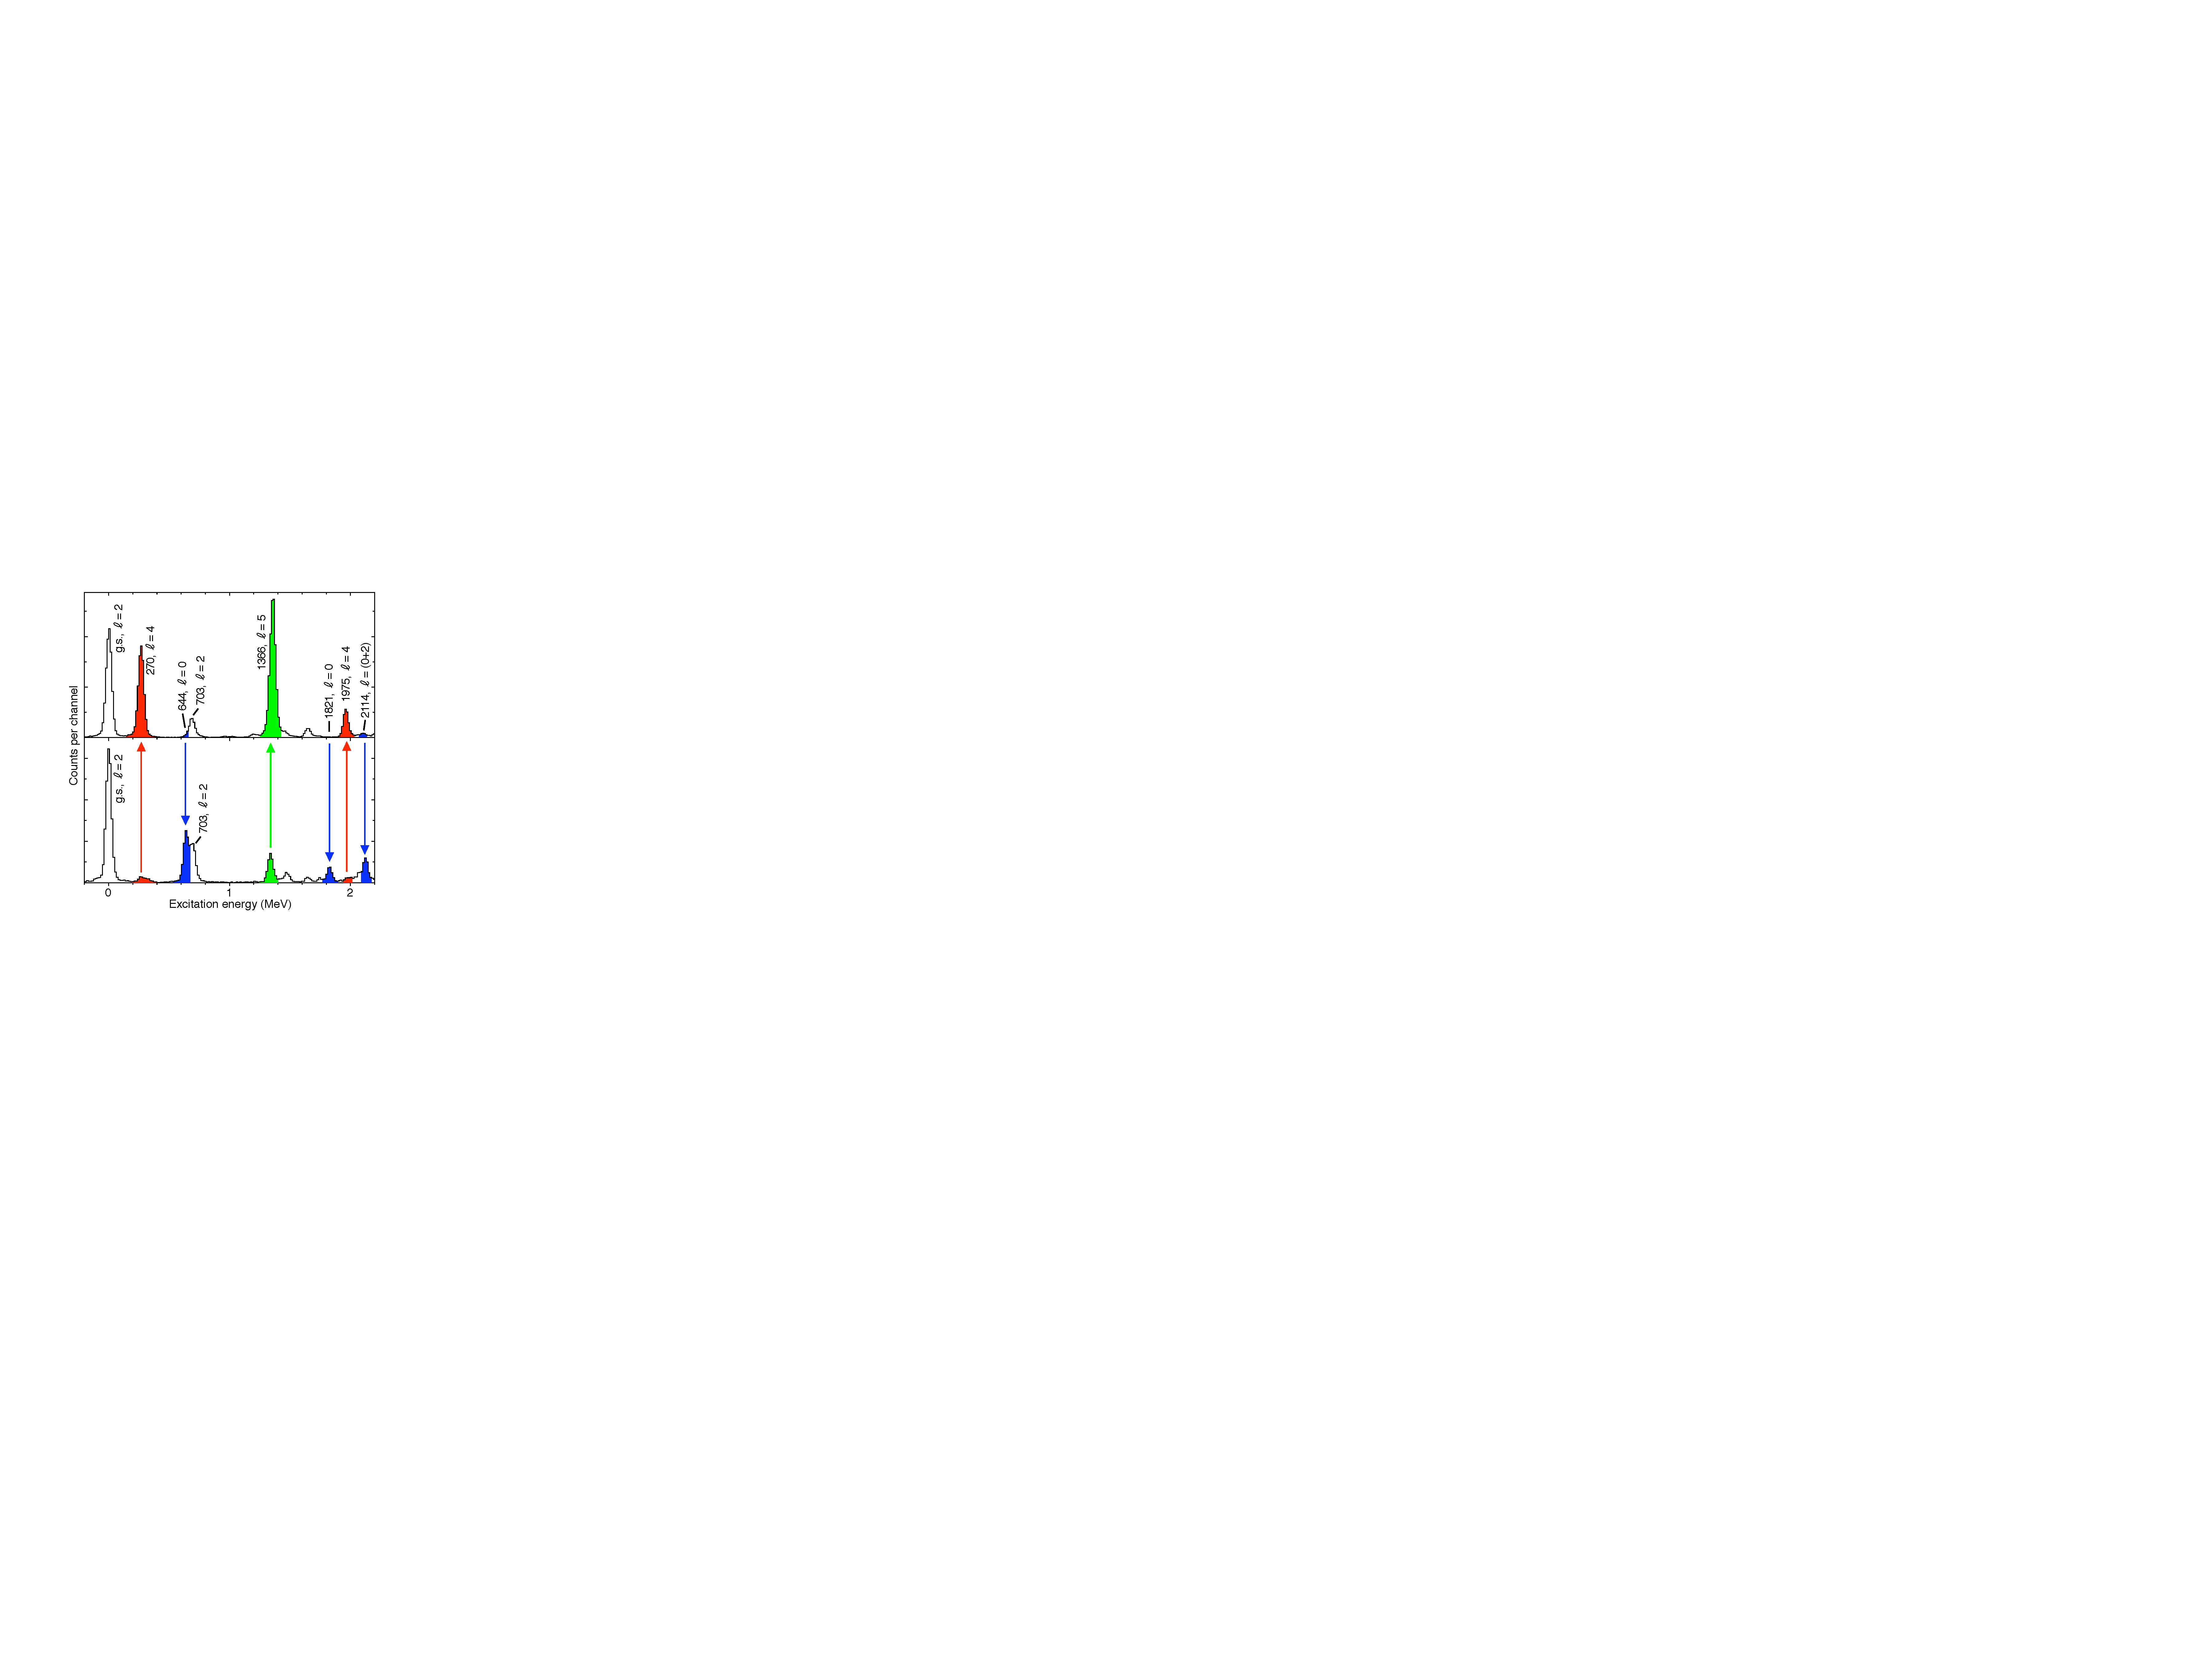
\includegraphics[width=\columnwidth,height=0.4\textheight,keepaspectratio]{matching_plot}%
\caption[Demonstration of momentum matching with two proton-stripping reaction on $^{118}$Sn]{Demonstration of momentum matching with two different proton-stripping reactions on $^{118}$Sn.  (Top) The $^{118}$Sn($\alpha$,$t$)$^{119}$Sb reaction, which has a large, negative $Q$-value of -14.7\,MeV, has enhanced yield to transitions corresponding to momentum transfers of $\ell=4$ and $\ell=5$. (Bottom) The yield to higher-spin states populated with the $^{118}$Sn($^3$He,$d$)$^{119}$Sb reaction is reduced and the low-spin states are enhanced.  Figure by B.~P.\ Kay from Ref.~\cite{Kay_2010PC}}%
\label{l_matching_spectra}%
\end{figure}

Continuing further with a naive picture of nuclear scattering, if the effects of the Coulomb field are neglected, the incoming plane-wave can be modeled as scattering from a hard sphere.  The Fraunh\"ofer diffraction equation
\begin{equation}
f(\theta)=\frac{ik}{4\pi}(1+\cos \theta)\int_S{e^{(i\vec{q}\cdot \vec{r})}dS}
\label{eq:1}
\end{equation}
gives the scattering amplitude as a function of angle and momentum transfer~\cite{Satchler_1990}.  Rewritten in terms of a differential cross section, this relationship becomes
\begin{equation}
\frac{d \sigma}{d \Omega}=k^2 r_0^4 \left[\frac{j_\ell(kr_0\theta)}{kr_0\theta}\right]^2
\label{eq:3}
\end{equation}
where $j_\ell(kr_0\theta)$ spherical Bessel function of order $\ell$.  
%Many nuclear properties have been studied by bombarding heavy nuclei with beams of light ions.  
This relationship shows that measuring the angular variations in the intensity of the energy levels provides additional useful information.  There is a direct relationship between the angular momentum $\ell$ transferred to the heavy recoil and the angular distribution of the ejected particle.  The resultant angular distribution is proportional to $j_\ell(kr_0\theta)$. Fig.~\ref{si_ang} shows an example of angular distributions from the $^{28}$Si($d$,$p$)$^{29}$Si reaction which exhibit an interference pattern comparable to Eq.~\ref{eq:3}.

\begin{figure}%
\centering
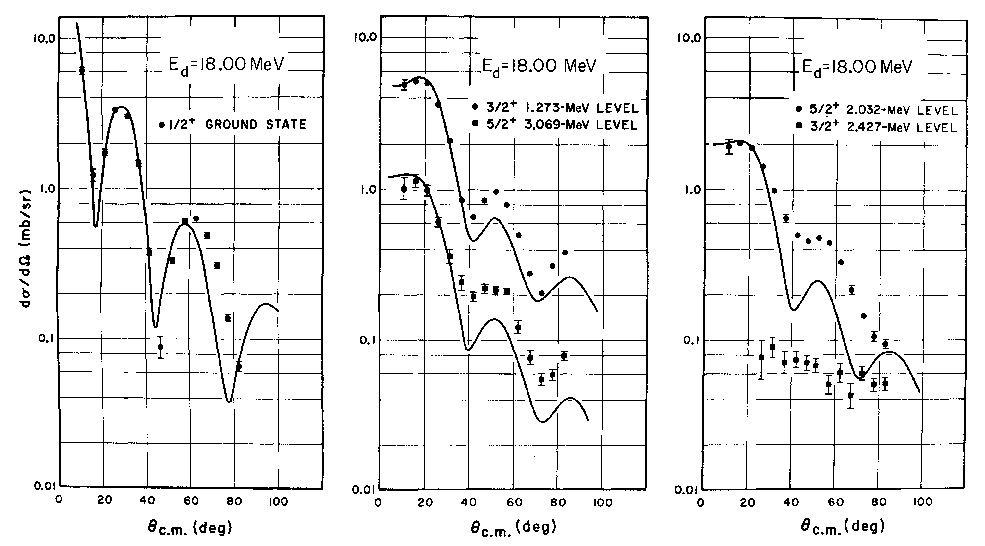
\includegraphics[width=\columnwidth]{Mermaz_fig_2}
\caption[Angular distributions from the $^{28}$Si($d$,$p$)$^{29}$Si reaction in normal kinematics]{Angular distributions from the $^{28}$Si($d$,$p$)$^{29}$Si reaction in normal kinematics.  Shown here are the angular distributions of four levels populated in the $^{28}$Si($d$,$p$)$^{29}$Si reaction at 9\,\AMeV{} with DWBA fits.  Figure from \citet[Fig.~1]{Mermaz_1971}.}
\label{si_ang}
\end{figure}

\section{Optical Model}
The phenomenological optical model was developed to improve upon the limitations of the plane wave theory of reactions.  The optical model characterizes the reaction by a potential which \textit{distorts} the incoming and outgoing plane waves.
\subsection{Nuclear Potentials}
%\subsubsection{Coloumb}
The optical model potential approximates the nuclear potential as
\begin{equation}
U(r)=-V f(r,r_0,a)-iW f(r,R^\prime,a^\prime)-iW_D g(r,r_0^\prime,a^\prime)
\label{eq:optical_im}
\end{equation}
where $V$ depths of the real parts of the Woods-Saxon potential, $W$ is the depth of the imaginary (absorption) part of the Woods-Saxon potential and $W_D$ is the strength surface-peaked imaginary potential.  The surface potential $g(r)$ is given by the derivative of the Woods-Saxon potential.
\begin{equation}
g(r,r_0^\prime,a^\prime)=4a\frac{d}{dr}f(r,r_0^\prime,a^\prime)
\label{eq:surface}
\end{equation}
In a similar fashion, the radial dependence of the spin-orbit term in Eq.~\ref{eq:woods_saxon} may be rewritten in terms of $g_\mathrm{SO}=r^{-1}(d/dr)f(r,r_\mathrm{SO},a_\mathrm{SO})$.  The exact depths of the real potentials are varied to reproduce the previously-known nucleon separation energy for a given nucleus.  The potential given in Eq.~\ref{eq:optical_im} includes imaginary terms in order to allow the removal of flux from the elastic scattering channel, \textit{i.e.}, for inelastic scattering.
%\subsection{Partial Wave Analysis}
\subsection{Distorted Wave Born Approximation}
\label{dwba}
Except for a number of special cases, the solutions to the Schr\"odinger equation for the optical model potential do not have a closed form and require computational solutions~\cite{Glendenning_2004}.  Calculating transition amplitudes for direct reactions in this way is called the distorted-wave Born approximation (DWBA).  By comparing the measured shape of the angular distributions from an experiment to DWBA calculations, the angular momentum transfer $l$ can be determined and the degree to which the states are accurately described as a single-particle state.  This provides a clear way of assigning the spin to the states populated in the heavy recoil.  The relationship between the measured angular distribution  and the calculated angular distribution is given by

\begin{equation}
\left(\frac{d\sigma}{d\Omega}\right)_\textrm{meas}=S\left(\frac{d\sigma}{d\Omega}\right)_\textrm{DWBA}
\label{eq:}
\end{equation}
where $S$ is called the spectroscopic factor.  For a state perfectly describe as a nucleon orbiting an closed core, that is, a single-particle state, the spectroscopic factor is identically equal to one.  The spectroscopic factor provides a measure of the overlap between the final state and the initial state plus an added nucleon.  Fig.~\ref{dwba_ediff} shows an example of calculations using the finite-range DWBA code PTOLEMY~\cite{Macfarlane_1978} using optical model parameters from Chapt.~\ref{exp} for the $^{28}$Si($d$,$p$) reaction at a variety of bombarding energies.

\begin{figure}%
\centering
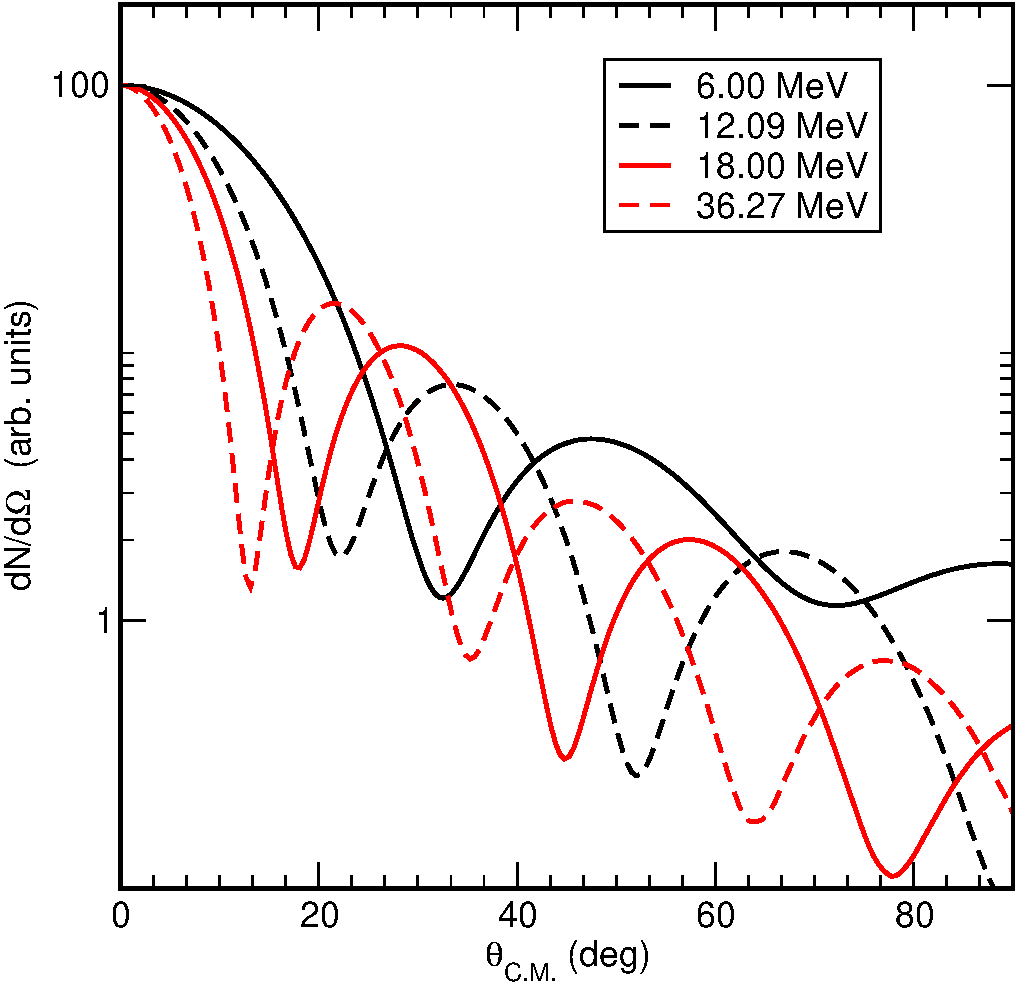
\includegraphics[width=\columnwidth,height=0.4\textheight,keepaspectratio]{angdist_curves_ediff}%
\caption[DWBA calculations for the $^{28}$Si($d$,$p$) reaction at four different bombarding energies]{DWBA calculations for the $^{28}$Si($d$,$p$) reaction at four different bombarding energies.  The calculations were carried out for the $\ell_n=0$ transitions to the $^{29}$Si ground state using the code PTOLEMY.  The cross sections have been normalized to $dN/d\Omega=100$ at $\theta_\mathrm{cm}$.}%
\label{dwba_ediff}%
\end{figure}

\section{Conclusion}
With few exceptions, most stable-beam stable-target combinations have been studied in terms of nucleon transfer reactions.  In order to measure the properties of nuclei further away from stability, it is necessary to utilize either radioactive beams or radioactive targets.  In principle, this technique would be useful to study exotic nuclei.  In terms of the $r$-process, it would be particularly useful to study neutron-rich nuclei with the ($d$,$p$) reaction which deposits a neutron on the target nucleus.  However, the nuclei of interest are so unstable that they are unsuitable for making targets.  Until recently, this limitation has made transfer reactions inapplicable to the study of exotic nuclei.  With the arrival of rare isotope beam capabilities at nuclear accelerator facilities, exotic nuclei can now be studied with this powerful technique.

The worldwide development of radioactive ion beam facilities is allowing for a new generation of nuclear reactions to be studied.  Reactions utilizing such exotic beams are permitting measurements of nuclear properties further away from stability than previously possible.  With radioactive beams, however, the kinematics of the measurement must be inverted, with a heavy-ion beam bombarding a light-ion target.  The basic form of the reactions being studied is the same (nucleon stripping or knock-out), but the reaction kinematics are changed in a way which presents new measurement difficulties.

%\section{Observables}
%
%\subsection{Angular Distribution}
%
%\subsection{Cross Section}
%\subsubsection{Spectroscopic Factor}
%
%Overlap between initial and final states.  Comparison between theory and experiment.  A measure of the single particle strength of the orbit. %\cite{Jiang_2009}
%\subsubsection{Selectivity}
%preferentially populates states with single-particle nature.~\cite{Wuosmaa_2005PRC,Wuosmaa_2008}
\part{Experimental Techniques}
\chapter{Two-body Kinematics}
\label{chapt:kin}
Direct nuclear transfer reactions, as discussed in the previous chapter, can be described in terms of two-body kinematics.  The feature that makes the HELIOS spectrometer unique is the effect that the spectrometer's magnetic field has on the  motion of the reaction products (solenoidal transport) and the way in which the products are measured (detector geometry).  Therefore, in order to have a meaningful discussion of the benefits of HELIOS, it is necessary to introduce the key concepts of reaction kinematics.  This chapter also discusses the specific challenges encountered when measuring reaction in inverse kinematics.  
\section{Basic Principles}
Reaction kinematics form a subset of generalized two-body kinematics.  In the typical %\note{accelerator-target}
setup, a beam of ions of mass $m_1$ are accelerated to a velocity of $v_1$ and bombard stationary target atoms of mass $m_2$.  In ``normal kinematics'' a light ion beam strikes a heavy ion target with $m_1<m_2$.  An example of such a reaction is the $^{28}$Si($d$,$p$) as discussed in Ref~\cite{Mermaz_1971}, in which a deuteron beam strikes a silicon target.  In ``inverse kinematics'' the masses are reversed---a heavy ion beam strikes a light ion target ($m_1>m_2$).  The same ($d$,$p$) reaction on silicon is written in inverse kinematics as $d$($^{28}$Si,$p$).  This is the reaction presented in Ref.~\cite{Lighthall_2010} and discussed in Chapt.~\ref{exp}.
\subsection{Energy}
Before the reaction, given a stationary target and an accelerated ion beam, the total kinetic energy of the two-body system in the laboratory frame is equal to the beam energy $E_1$.  
The total kinetic energy in the center-of-mass system is then given by
\begin{equation}
T_\mathrm{cm}=\frac{m_2}{m_1+m_2}E_1
\label{eq:total-energy}
\end{equation}
where $E_1=\frac{1}{2}m_1v_1^2$ is the kinetic energy of the beam particle.

The system then gains or loses energy depending on the specific reaction energy, referred to as the $Q$-value.  The $Q$-value will be defined here as the change in total energy of the system before and after the reaction in a ground-state transition.  With this definition, the reaction $Q$-value may be calculated as the change in mass.
\begin{equation}
Q=[(m_1+m_2)-(m+M)]c^2
\label{eq:q_value}
\end{equation}
where $Q$ is explicitly the energy \textit{gained} in the reaction\footnote{Some texts define the $Q$-value as the total amount of energy lost in the reaction, in which case $Q^\prime=-Q+E_x$.}.  Here the masses of the reaction products are written as $m$ and $M$, with $m<M$.  In this notation, an endothermic reaction will have a negative $Q$-value.  For transitions to states other than the ground-state, the excitation energy $E_x$ must also be included in calculating %$E_\mathrm{total}$, 
the resultant total kinetic energy in the center-of mass frame.
\begin{equation}
E_\mathrm{total}=T_\mathrm{cm}+Q-E_x
\label{eq:ecmtotal}
\end{equation}

With the energy $E_\textrm{total}$ defined above, the conservation of momentum gives the (non-relativistic) kinetic energy of the ejectile in the center-of-mass system as
\begin{equation}
\begin{split}
E_\mathrm{cm}&=E_\mathrm{total}\frac{M}{m+M}\\
&=\frac{1}{2}m v_0^2
\end{split}
\label{eq:ecm}
\end{equation}
where $v_0$ is the velocity of the ejectile (mass $m$) in the center-of-mass frame.

\subsection{Velocity}
%Two important constants of motion in two-body kinematics are the velocity of the center-of-mass $V_\mathrm{cm}$ and the %velocity of the light ion ejectile %of mass $m$
% in the center-of-mass frame $v_0$. 
The center-of-mass system is defined as the reference frame in which the reactants have equal and opposite momentum vectors.
%In the center-of-mass system, the colliding particles have equal momentum by definition.
In the laboratory system, this center-of-mass has a velocity %of the center-of-mass $V_\mathrm{cm}$  
given by
\begin{equation}
\begin{split}
V_\mathrm{cm}&=v_{1}\frac{m_{1}}{m_{1}+m_{2}}.\\
%&=\sqrt{\frac{2 E_1}{m_1}}\frac{m_{1}}{m_{1}+m_{2}}
\end{split}
\label{Vcm}
\end{equation}
%where $V_1$ and $m_1$ refer to the beam particle and $m_2$ is the target particle.
The velocity of the ejectile (mass $m$) in the center-of-mass frame $v_0$ is given in terms of the total kinetic energy in the center-of-mass $E_\textrm{total}$.  Substituting Eq.~\ref{eq:ecmtotal} into Eq.~\ref{eq:ecm} and solving for $v_0$ yields
\begin{equation}
\begin{split}
v_0%&=\sqrt{\frac{2 E_\mathrm{cm}}{m}}\\
&=\sqrt{\frac{2M(T_\mathrm{cm}+Q-E_x)}{m(m+M)}}.
\end{split}
\label{kin_v0}
\end{equation}

The velocity magnitudes $V_\mathrm{cm}$ and $v_0$ are constants of motion.  Eq.~\ref{Vcm} shows that for a given reaction, $V_\mathrm{cm}$ is fixed by the bombarding energy of the beam particle.  Similarly, Eq.~\ref{kin_v0} shows that $v_0$ is fixed by the reaction $Q$-value and transition energy $E_x$, in addition to the bombarding energy.
These velocities are related to the laboratory velocity by $\vec{v_\mathrm{lab}}=\vec{V_\mathrm{cm}}+ \vec{v_0}$.  The magnitude $v_\mathrm{lab}$ varies as the emission angle $\theta_\mathrm{cm}$ changes.  %This transformation between the laboratory system and the center-of-mass system is visualized graphically in Fig.~\ref{big_kin}.  
With reference to Fig.~\ref{big_kin}, the magnitude $v_\mathrm{lab}$ is readily obtained using the law of cosines
\begin{equation}
v_\mathrm{lab}^2=v_0^2+V_\mathrm{cm}^2-2v_0 V_\mathrm{cm}\cos(180^\circ - \theta_\mathrm{cm}).
\label{eq:law_of_cosines}
\end{equation}
Rewriting in terms energy, one gets
\begin{equation}
\begin{split}
E_\mathrm{lab}%&=\frac{1}{2} m\left[v_0^2+V_\mathrm{cm}^2 +2V_\mathrm{cm}v_0 \cos(\theta_\mathrm{cm})\right]\\
&=E_\mathrm{cm}+\frac{1}{2} m V_\mathrm{cm}^2 +m V_\mathrm{cm}v_0 \cos(\theta_\mathrm{cm}).
\end{split}
\label{elab}
\end{equation}
 %with $v_\mathrm{lab}$ derived from the measured energy, $V_\mathrm{cm}$ set by the beam energy, and $v_0$ is determined by beam energy, the Q-value of the reaction, and the excitation energy.

\begin{figure}%
\centering
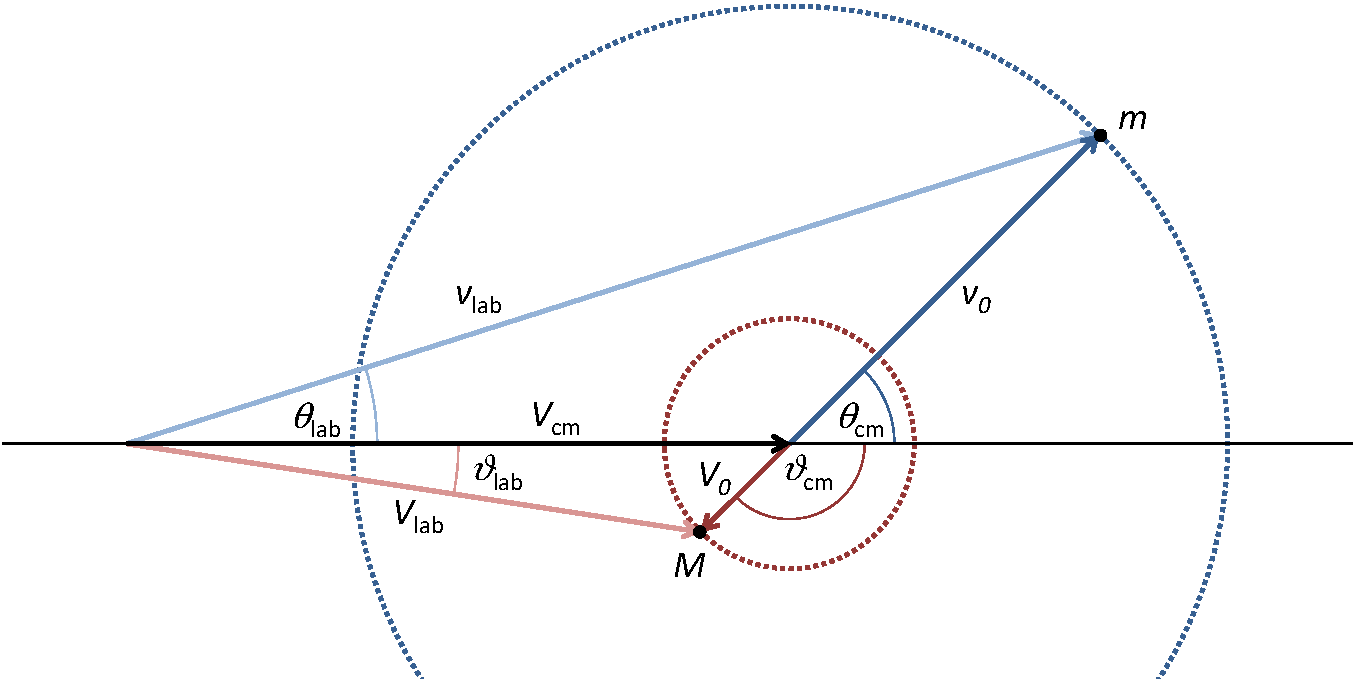
\includegraphics[width=\columnwidth]{kin_fig_3c}
\caption[Transformation of velocities between the laboratory and the center-of-mass systems]{Transformation of velocities between the laboratory and the center-of-mass systems. As the ejection angle of mass $m$ varies (large circle) from $\theta_\mathrm{cm}=0$--$180^\circ$, the particle is scattered at an angle of $\theta_\mathrm{lab}$ such that $\vec{v_\mathrm{lab}}=\vec{V_\mathrm{cm}}+\vec{v_0}$.
  Mass $M$ is ejected such that $\theta_\mathrm{cm}+\vartheta_\mathrm{cm}=180^\circ$.
Adapted from \citet[Fig.~11]{Michalowicz_1967}.}
\label{big_kin}%
\end{figure}

\subsection{Angle}
After the reaction, the ejectile is emitted at an angle in the center of mass $\theta_\mathrm{cm}$ over the range of 0--180$^\circ$.  Due to the conservation of momentum, the ejectile and the heavy recoil are ejected back-to-back in the center-of-mass frame with $\theta_\mathrm{cm}+\vartheta_\mathrm{cm}=180^\circ$% (refer to Fig.~\ref{big_kin})
.  To be consistent with the convention used in most textbooks, the center-of-mass angle $\theta_\mathrm{cm}$ is defined relative to $+V_\textrm{cm}$ direction, as illustrated in Fig.~\ref{big_kin}.  This choice of coordinates is natural in normal kinematics where, in the rest frame of the heavy ion target, the beam is approaching at a velocity of $\approx v_1$.  However, in inverse kinematics %, in the rest frame of the heavy ion beam, 
the target is approaching the heavy ion at a \textit{negative} velocity of $-V_\mathrm{cm}$.  Therefore, in inverse kinematics% To account for this disparity
, the center-of-mass angle is defined as the compliment of the angle shown in Fig.~\ref{big_kin} ($180^\circ-\theta_\mathrm{cm}$).  Thus in both cases, $\theta_\textrm{cm}=0^\circ$ refers to the light ion traveling in the same direction before and after the reaction from the standpoint of the heavy ion.

In the laboratory frame, the extent to which $\theta_\mathrm{lab}$, and in turn $E_\mathrm{lab}$, vary as a function of $\theta_\textrm{cm}$ depends on how $V_\mathrm{cm}$ and $v_0$ compare to one another.  The value of the ratio $K=V_\mathrm{cm}/v_0$ divides the reactions into three classes.  Table~\ref{k_factors5} gives the $K$-values for a number of reactions.

\begin{table*}%[ht]
  \centering
  \begin{tabular}{,....c}		
    \hline
    \multicolumn{1}{c}{\multirow{2}{*}{Reaction}}  &  
    \multicolumn{1}{c}{$Q$-value}  &
    \multicolumn{1}{c}{$E_1/A_1$}  &  
    \multicolumn{1}{c}{$K_\mathrm{g.s.}$}  &  
    \multicolumn{1}{c}{$\theta_\mathrm{max}$} & Ref. \\%\cline{2-6}
    &\multicolumn{1}{c}{(MeV)}  &\multicolumn{1}{c}{(\AMeV)}  &   &\multicolumn{1}{c}{(deg)} & \\
    \hline \hline 
		^{132}\textrm{Sn}(d,p)^{133}\textrm{Sn}  &0.25&  4.78  &  0.01  &  180.0  & \textit{unstable}\\
		^{124}\textrm{Sn}(d,\textrm{He}^3)^{123}\textrm{In}  &-6.61&  14.35  &  0.02  &  180.0  & \cite{Weiffenback_1971}\\
		^{28}\textrm{Si}(d,p)^{29}\textrm{Si}  &6.25&  8.94  &  0.04  &  180.0  & \cite{Mermaz_1971} \\
		^{12}\textrm{B}(d,p)^{13}\textrm{B}  &2.65&  6.24  &  0.10  &  180.0  &\textit{unstable}\\
		d(^{28}\textrm{Si},p)^{29}\textrm{Si}  &6.25&  6.02  &  0.56  &  180.0  & \cite{Lighthall_2010} \\
		d(^{12}\textrm{B},p)^{13}\textrm{B}  &2.65&  6.24  &  0.61  &  180.0  &\cite{Lee_2010,Schiffer_2010}\\
		d(^{132}\textrm{Sn},p)^{133}\textrm{Sn}  &0.25&  4.78  &  0.70  &  180.0  & \cite{Pain_2007,Jones_2007,Pain_2008,Jones_2010} \\
		d(^{124}\textrm{Sn},^3\textrm{He})^{123}\textrm{In}  &-6.61&  13.00  &  1.42  &  44.6  &\textit{proposal}\\
	  \hline
  \end{tabular}
  \caption[Ground-state transition velocity ratios $K_\mathrm{g.s.}$ for a number of reactions]{Ground-state transition velocity ratios $K_\mathrm{g.s.}$ for a number of reactions.  For each reaction, the values are given for both normal and inverse kinematics.  For reactions that have been performed, the beam energy has been selected to match the given reference.}
  \label{k_factors5}
  \end{table*}

\begin{figure}[ht]
\begin{center}
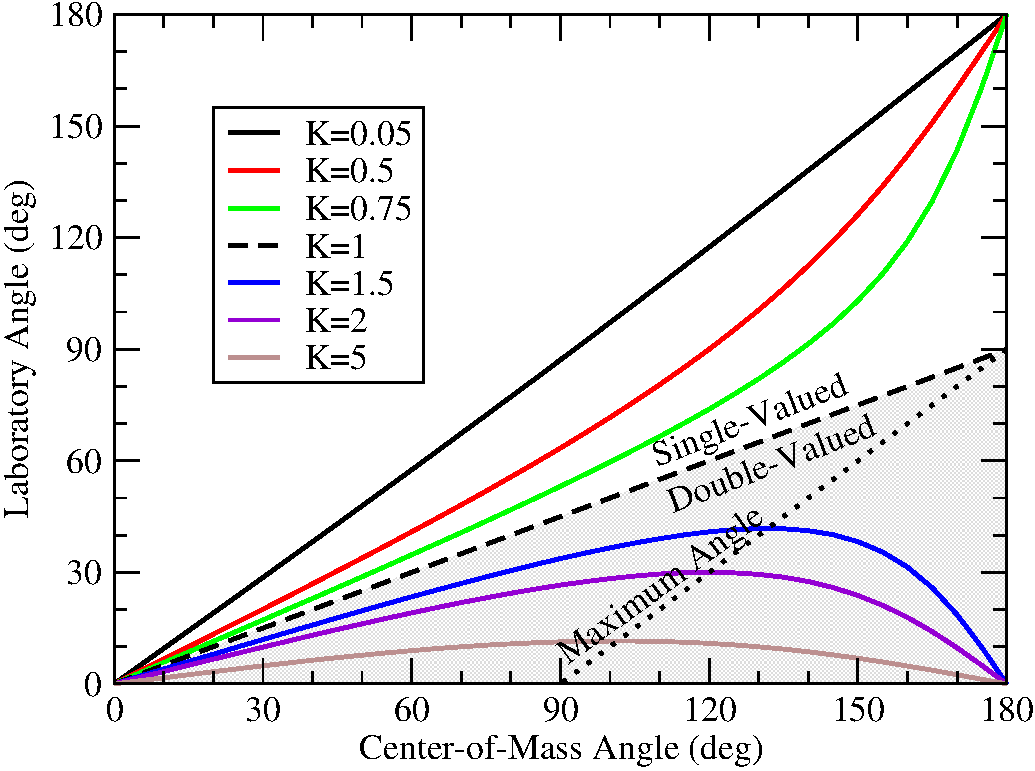
\includegraphics[keepaspectratio,width=\columnwidth,height=0.5\textheight]{angles34}%	
\end{center}
\caption[Transformation of angles between the laboratory and the center-of-mass systems]{Transformation of angles between the laboratory and the center-of-mass systems.  For $K>1$ the transformation is double-valued in the laboratory.  The maximum laboratory angle for such solutions is plotted.  Adapted from \citet[Fig.~9]{Michalowicz_1967}.}%
\label{angles}%
\end{figure}

\subsubsection{$K<1$}
For $K<1$ the laboratory energy $E_\mathrm{lab}$ is a single-valued function of the laboratory angle $\theta_\mathrm{lab}$, with the ejectile being emitted over all laboratory angles.  In the limit of normal kinematics, %the scattered beam ion, which is the light reaction product, is detected.  W
when the beam is much lighter than the target ($m_1 \ll m_2$), the center-of-mass of the reaction system is nearly at rest.  Eq.~\ref{elab} shows that when the velocity ratio $K \ll 1$---that is, when $V_\mathrm{cm} \ll v_0$---the laboratory energy $E_\mathrm{lab}$ begins to lose its dependence on the angle $\theta_\mathrm{cm}$.  This relationship is shown in Fig.~\ref{angles} by the line $K=0.05$ illustrating $\theta_\mathrm{lab}\approx \theta_\mathrm{lab}$.
  
As the ratio $K$ becomes comparable to 1, the reactions enter the realm of inverse kinematics.  The laboratory energy $E_\mathrm{lab}$ varies strongly with angle as the $\cos (\theta_\mathrm{cm})$ term in Eq.~\ref{elab} begins to dominate.  When $V_\mathrm{cm}$ and $v_0$ are more aligned, the energy in the laboratory $E_\mathrm{lab}$ is large compared to the energy in the center-of-mass $E_\mathrm{cm}$.  This corresponds to forward angles in the laboratory; at rearward angles, the inverse is true. 

\subsubsection{$K=1$}
\label{kisone}
$K_\mathrm{g.s.}=1$ is the trivial case, arising in two ways.  First, in elastic scattering, corresponding to $Q=E_x=0$; and second, when $E_x\approx Q+E_1/A_1$.  When no energy is transferred in the reaction, $V_\mathrm{cm}=v_0$ and $\theta_\mathrm{lab}=\frac{1}{2}\theta_\mathrm{cm}$.  The ejectile is emitted in the forward hemisphere only, with $\theta_\textrm{lab} \leq 90^\circ$.  This relationship is shown in Fig.~\ref{angles} by the line $K=1$.
\subsubsection{$K>1$}
For $K>1$, when $v_0<V_\mathrm{cm}$, the ejectile cannot be emitted in the rearward hemisphere.  Thus,  the laboratory energy $E_\mathrm{lab}$ is a double-valued function of the laboratory angle $\theta_\mathrm{lab}$ and the ejectile is emitted over a limited range of angles in the forward hemisphere.  The ejectile has a maximum emission angle in the laboratory given by
\begin{equation}
\theta_\mathrm{max}=\tan^{-1}\left(\frac{1}{\sqrt{K^2-1}}\right)=\sin^{-1}\left(\frac{1}{K}\right)
\label{max_theta}
\end{equation}
The shaded region of Fig.~\ref{angles} illustrates the relationship between $K$ and $\theta_\mathrm{max}$ and Table~\ref{k_factors5} gives $\theta_\mathrm{max}$ for a specific reaction in inverse kinematics.
In such cases, each angle $\theta_\mathrm{lab}$ corresponds to a ``high energy'' solution and a ``low energy'' solution.  The low energy solution corresponds to particles emitted at more forward angles (typically $\theta_\textrm{cm} \lesssim 30^\circ$) in the center-of-mass frame.

In the limiting case of $K \gg 1$, when $V_\textrm{cm} \gg v_0$, Eq.~\ref{elab}  again shows that the laboratory energy $E_\textrm{lab}$ will lose its dependence on the angle $\theta_\textrm{cm}$.  However, in this case, the laboratory velocity is approximately the center-of-mass velocity $v_\textrm{lab}\approx V_\textrm{cm}$.  This is the typical situation for the heavy ion reaction product.  Furthermore, in the limit of inverse kinematics ($m_1\gg m_2$), the velocity of the heavy recoil is then also approximately the incident beam velocity $V_\textrm{lab}\approx V_\textrm{cm} \approx v_1$.  

\section{Inverse Kinematics}
The utility of studying reactions in inverse kinematics is that it provides access to measurements involving heavy isotopes that are unstable against $\beta$-decay.
However, as detailed in the previous section, the transition to inverse kinematics is not simply a reversal of target and beam.  The rapidly changing laboratory quantities that are encountered have serious implications for measurements carried out in inverse kinematics.  In addition, the difficulties associated with a radioactive ion beam must also be considered.  This section discusses several of these challenge.
 
\subsection{Kinematic Compression}
\label{kin_comp}
In inverse kinematics, the center-of-mass of the reaction has a substantial velocity in the laboratory frame.  When the velocity of the light ion reaction product $v_0$ is comparable to the velocity of center-of-mass $V_\mathrm{cm}$, the energies of the emitted light ions are highly angle-dependent.  When these velocities are anti-aligned (forward center-of-mass angles), the laboratory energy is significantly smaller than in normal kinematics.  This also has the effect of compressing the relative spacing between energy levels at a given $\theta_\mathrm{lab}$.

\subsubsection{Compression Coefficient}
The separation between two energy levels in the laboratory frame is defined here as $\Delta E_\mathrm{lab}=(E_\mathrm{lab}-E_\mathrm{lab}^\prime)$.  Starting with Eq.~\ref{elab} and holding $V_\mathrm{cm}$ and $\theta_\mathrm{cm}$ constant, the energy separation in the laboratory at a fixed emission angle is given by
\begin{equation}
\begin{split}
\Delta E_\mathrm{lab}
&=\Delta E_\mathrm{cm}+mV_\mathrm{cm}\Delta v_0 \cos(\theta_\mathrm{cm})
\end{split}
\label{eq:delta_e2}
\end{equation}
The energy separation in the center-of-mass frame is given by
\begin{equation}
\begin{split}
\Delta E_\mathrm{cm}
&=\frac{1}{2}m \Delta (v_0)^2\\
&=\frac{1}{2}m (v_0+v_0^\prime)\Delta v_0
\end{split}
\label{eq:delta_ecm}
\end{equation}
The ratio of the separation of the energy levels in the laboratory $\Delta E_\mathrm{lab}$ to that in center-of-mass will be defined here as the ``compression coefficient''
\begin{equation}
\begin{split}
\frac{\Delta E_\mathrm{lab}}{\Delta E_\mathrm{cm}}
&=\frac{\Delta E_\mathrm{cm}+mV_\mathrm{cm}\Delta v_0 \cos(\theta_\mathrm{cm})}{\frac{1}{2}m (v_0+v_0^\prime)\Delta v_0}\\
&=1+\frac{2V_\mathrm{cm}\cos(\theta_\mathrm{cm})}{(v_0+v_0^\prime)}\\
&=1+\frac{2 K \cos(\theta_\mathrm{cm})}{(1+v_0^\prime/v_0)}
\end{split}
\label{eq:compress}
\end{equation}
and is identically equal to $1$ at $\theta_\mathrm{cm}=90^\circ$.  For reactions in normal kinematics, with $K \ll 1$, this effect is suppressed and $\Delta E_\mathrm{lab}/\Delta E_\mathrm{cm}\approx 1$ for all angles.  In both normal and inverse kinematics, at rearward emission angles ($\theta_\mathrm{cm}>90^\circ$) the effect causes an increase of the energy spacing ($\Delta E_\mathrm{lab}/\Delta E_\mathrm{cm}> 1$).  
However, in order to differentiate the angular distributions associated with different angular momentum transfers, it is necessary to measure the reactions at forward angles ($\theta_\textrm{cm} \lesssim 30^\circ$).  This region of interest is where the effect of kinematic compression is the most dramatic.  
In cases when the $K$-value of the reaction is $>1$, meaning the laboratory energy $E_\mathrm{lab}$ is a double-valued function of the laboratory angle $\theta_\mathrm{lab}$, the value of $\Delta E_\mathrm{lab}/\Delta E_\mathrm{cm}$ is negative for the low energy solution.  In some cases,  the low energy solution will also see an enhancement in the energy level spacing ($\Delta E_\mathrm{lab}/\Delta E_\mathrm{cm}< -1$) at the most forward laboratory angles.

\subsubsection{Example}
Fig.~\ref{sn-plots} shows calculated plots of energy $E_\textrm{lab}$ vs. angle $\theta_\textrm{lab}$ %in the laboratory 
for the ($d$,$p$) reaction on $^{132}$Sn at 4.78\,\AMeV.  This bombarding energy is chosen to match the measurement of \citet{Jones_2010}.  This reaction is a benchmark measurement for inverse kinematics, not only because of the importance of the physics associated with the measurement (see Chapt.~\ref{astro}), but also because of the difficulty of the measurement.  In the figure, fictitious energy levels have been selected such that $\Delta E_x=1.0$\,MeV to illustrate kinematic compression.

$^{132}$Sn is unstable against $\beta$-decay with a half-life of $T_{1/2}=39.7$\,s.  Therefore it is impossible to make a $^{132}$Sn target for a reaction study in normal kinematics.  However, if it \textit{were} possible to perform this reaction in normal kinematics (left panel), the ground state transition would have a velocity ratio of $K_\mathrm{g.s.}=0.01$ and at $\theta_\mathrm{cm}=10^\circ$ the ``compression'' coefficient is $1.01$.  In inverse kinematics, the ground state transition has a velocity ratio of $K_\mathrm{g.s.}=0.70$ and at $\theta_\mathrm{cm}=10^\circ$ the compression coefficient is $0.30$.  Furthermore, in inverse kinematics, for excitation energies $E_x \gtrsim (Q+E_1/A_1)$, in this case $\approx 5$\,MeV, the energy solution is double-valued ($K>1$).  

\begin{figure}[ht]
\centering
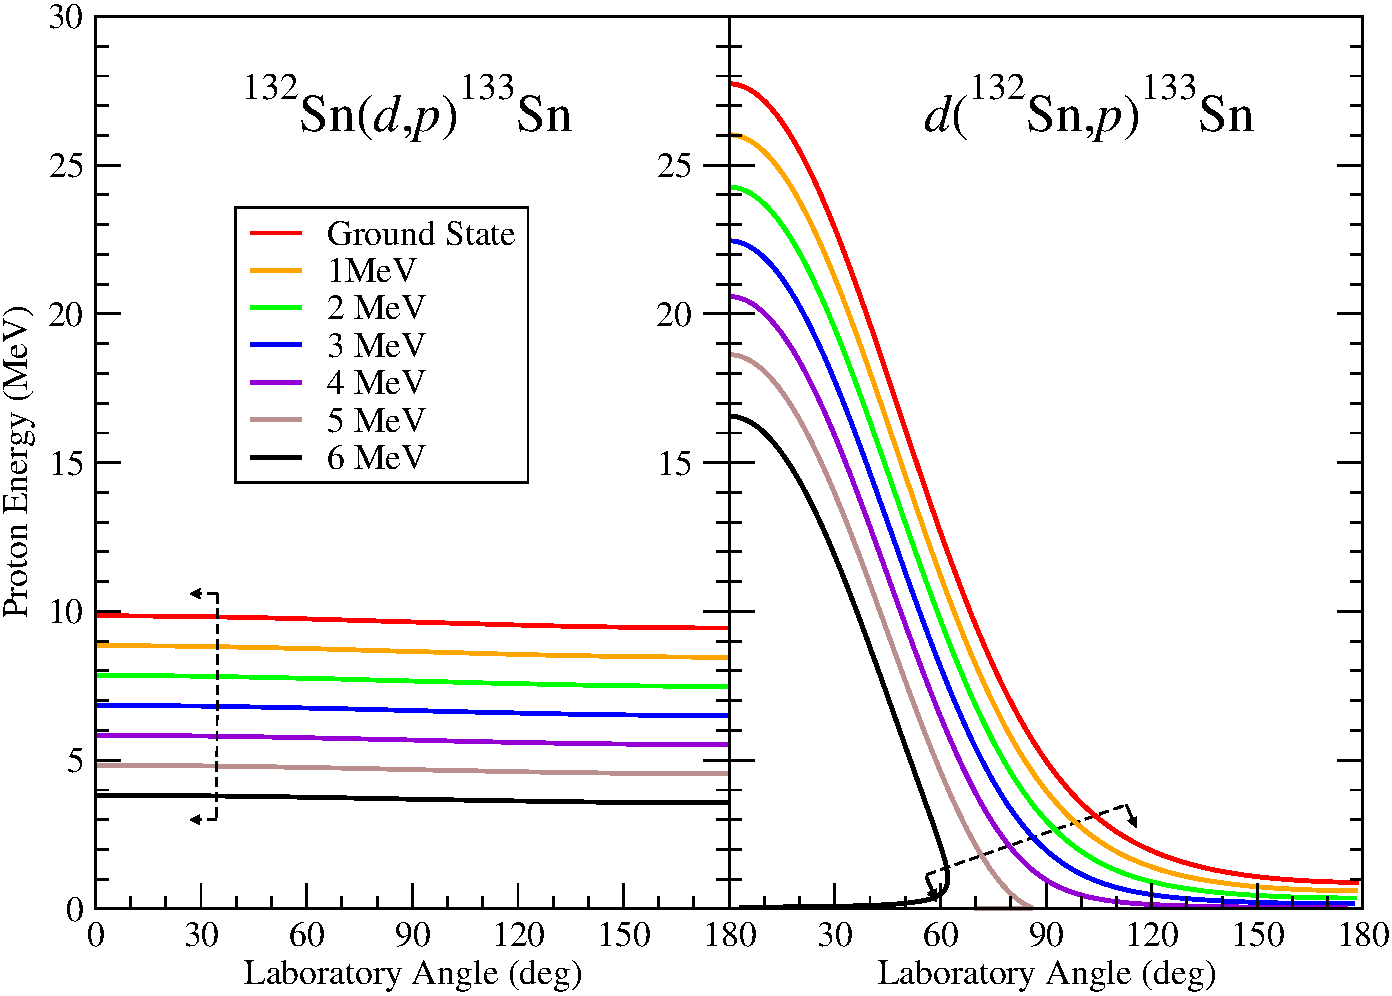
\includegraphics[width=\columnwidth,height=0.45\textheight,keepaspectratio]{sn132-plots3b}
\caption[Illustration of kinematic compression]{Illustration of kinematic compression.  In normal kinematics (left, $K_\mathrm{g.s.}=0.01$), the energy level spacing approximately constant and equal to the spacing in the center-of-mass.  In inverse kinematics (right, $K_\mathrm{g.s.}=0.70$), the energy spacing is dramatically compressed at forward angles, corresponding to emission in the rearward hemisphere.  The dashed lines indicate the approximate position of $\theta_\mathrm{cm}=35^\circ$, with the arrows indicating forward angles in the center-of-mass.  Note the laboratory energy $E_\mathrm{lab}$ becomes double-valued in inverse kinematics for $E_x > 5$\,MeV.}%
\label{sn-plots}%
\end{figure}

\subsection{Kinematic Broadening}
\label{kin_broad}
The effect of kinematic compression emphasizes the need for high-resolution energy measurements in inverse kinematics.  In addition, due to the strong dependence of the light recoil energy $E_\mathrm{lab}$ on laboratory angle $\theta_\mathrm{lab}$, it becomes essentially important to have precise angle measurement.  % in inverse kinematics.
Even in a system with perfect energy resolution ($\delta E_\mathrm{lab}=0$), the range of angles covered by a finite detector element $\delta \theta_\mathrm{lab}$ corresponds to a range in measured energy; thus leading to a reduced measured energy resolution.  This relationship is illustrated in Fig.~\ref{error_fig}.  For example, in the $d$($^{132}$Sn,$p$) reaction discussed above, at $\theta_\mathrm{cm}=10^\circ$ ($\theta_\mathrm{lab}=149^\circ$) the rate-of-change (\textit{i.e.} slope) of the ground state transition in the laboratory is $dE_\mathrm{lab}/d\theta_\mathrm{lab}=41$\,keV/deg; at $\theta_\mathrm{lab}=90^\circ$ this value increases to 168\,keV/deg.  This unavoidable feature is referred to as the ``kinematic broadening'' of the %center-of-mass
 energy resolution~\cite{Winfield_1997}.  Put another way, due to the covariance between energy and angle, the energy resolution %in the center-of-mass frame 
 can be limited by angular resolution and vice-versa.  This effect is discussed below and demonstrated in Fig.~\ref{kin_broad_fig}.
 
\begin{figure}%
%\includegraphics[width=\columnwidth]{error_fig}\\%
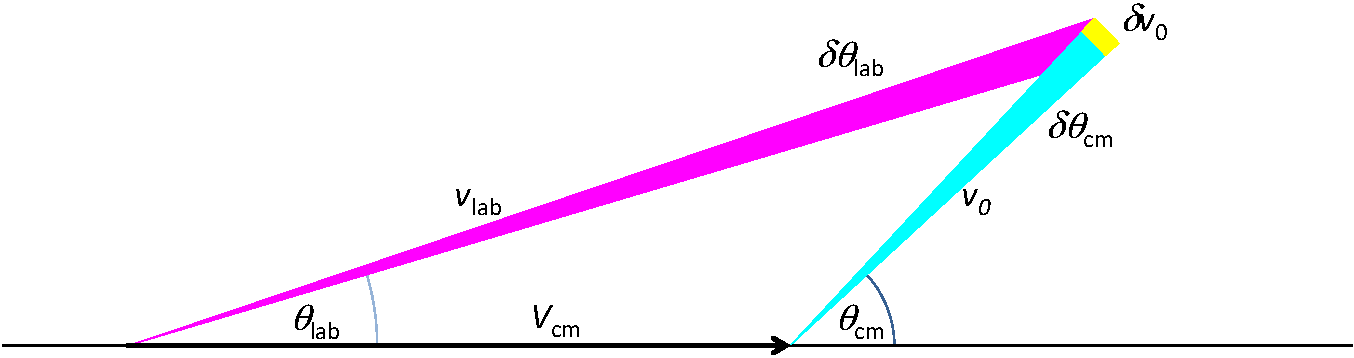
\includegraphics[width=\columnwidth]{error_fig2}%
\caption[Illustration of kinematic broadening]{Illustration of kinematic broadening.  For a fixed measurement of energy, an uncertainty in angle $\delta \theta_\mathrm{lab}$ leads to an uncertainty in both the (derived)  angle $\delta \theta_\mathrm{cm}$ and the energy (via $\delta v_0$).}%
\label{error_fig}%
\end{figure} 

\subsubsection{Resolution Propagation}
\label{res_prop}
The uncertainty of the measured quantity $\theta_\mathrm{lab}$ may lead to a kinematic broadening of the measured quantity $E_\mathrm{lab}$, as mentioned, but it also effects the derived quantities % in center-of-mass frame 
$E_\mathrm{cm}$ and $\theta_\mathrm{cm}$.  To see exactly how the measurement uncertainties effect the derived results, it is necessary to  perform an error analysis. 
%Through the region of interest, the center-of-mass angle changes more rapidly than the laboratory angle.  Therefore uncertainty in the center-of-mass angle is larger than the uncertainty in the laboratory angle.  The broadening of uncertainty lowers the final resolution of the center-of-mass energy spectrum.  This feature will always be present in an experiment measuring angle and energy to reconstruct inverse kinematics.
Solving Eq.~\ref{elab} for $E_\mathrm{cm}$ and rewriting in terms of the measured quantities $E_\mathrm{lab}$ and $\theta_\mathrm{lab}$ (this substitution is derived in Eq.~\ref{elab_of_vpara}) yields

\begin{equation}
\begin{split}
E_\mathrm{cm}&=E_\mathrm{lab}-\frac{1}{2} m V_\mathrm{cm}^2 -m V_\mathrm{cm}v_0 \cos(\theta_\mathrm{cm})\\
&=E_\mathrm{lab}+\frac{1}{2} m V_\mathrm{cm}^2 -m V_\mathrm{cm}v_\mathrm{lab} \cos(\theta_\mathrm{lab})\\
&=E_\mathrm{lab}+\frac{1}{2} m V_\mathrm{cm}^2 - V_\mathrm{cm}(\sqrt{2mE_\mathrm{lab}})\cos(\theta_\mathrm{lab})\\
\end{split}
\label{ecm3}
\end{equation}
Given this relationship, the uncertainty in $E_\mathrm{cm}$ due to the uncertainty in $E_\mathrm{lab}$ and $\theta_\mathrm{lab}$ can be calculated using the generalized error propagation equation~\cite{Bevington_2003,Drosq_2007}.
\begin{equation}
\begin{split}
\left(\delta E_\mathrm{cm}\right)^2&=\left(\frac{\partial E_\mathrm{cm}}{\partial E_\mathrm{lab}}\right)^2\left(\delta E_\mathrm{lab}\right)^2+\left(\frac{\partial E_\mathrm{cm}}{\partial \theta_\mathrm{lab}}\right)^2\left(\delta \theta_\mathrm{lab}\right)^2
%\\&\qquad
+2\left(\frac{\partial E_\mathrm{cm}}{\partial E_\mathrm{lab}}\right) \delta E_\mathrm{lab} \left(\frac{\partial E_\mathrm{cm}}{\partial \theta_\mathrm{lab}}\right)\delta \theta_\mathrm{lab}\\
\end{split}
\label{eq:delta_z4}
\end{equation}
The first two terms in this expression are the individual contributions of the two measured quantities, which are always positive.  The third term is the contribution of the covariance between the two quantities and can (mathematically) take on positive and negative values.  Each term is weighted by a partial derivative.  The weight for the uncertainty in energy $\delta E_\mathrm{lab}$ is given by
\begin{equation}
\begin{split}
\frac{\partial E_\mathrm{cm}}{\partial E_\mathrm{lab}}&=1-mV_\mathrm{cm}\cos(\theta_\mathrm{lab}) \sqrt{\frac{m}{2E_\mathrm{lab}}}
\end{split}
\label{eq:delta_E}
\end{equation}
and the weight for the uncertainty in angle $\delta \theta_\mathrm{lab}$ is given by
\begin{equation}
\begin{split}
\frac{\partial E_\mathrm{cm}}{\partial \theta_\mathrm{lab}}&=V_\mathrm{cm}\sqrt{2mE_\mathrm{lab}}\sin(\theta_\mathrm{lab}).
\end{split}
\label{eq:delta_theta}
\end{equation}

Thus using this technique, the contribution of the individual uncertainties in the measured quantities can be calculated.  Unless otherwise specified, the value of the uncertainties are characterized in terms of the full-width at half maximum (FWHM) $\Gamma$, as opposed to the standard deviation $\sigma$; the two are related by $\Gamma=2.35\sigma$.   Table~\ref{error_prop} shows the results of these calculations for a number of reactions in a manner similar to that presented by \citet{Winfield_1997}.  Following Ref.~\cite{Winfield_1997}, the contributions are calculated assuming measurement uncertainties of $\delta E_\mathrm{lab}=40$\,keV~FWHM, $\delta \theta_\mathrm{lab}=0.54^\circ$~FWHM and an uncertainty in the beam energy (discussed below) of 0.14\%.  However in Ref.~\cite{Winfield_1997}, the individual contributions are added in quadrature, neglecting the effects of the covariance of the measured quantities.  The two rightmost columns in Table~\ref{error_prop} show the sum of the uncertainties added quadratically $\Sigma_\textrm{quad}$ and the sum including the covariation term $\Sigma_\textrm{covar}$.  As expected, this contribution has little effect in normal kinematics where the covariance between $E_\mathrm{lab}$ and $\theta_\mathrm{lab}$ is negligible.  However, in inverse kinematics the contribution of the covariance is significant.  The last two rows of Table~\ref{error_prop} show that in some cases (when $K>1$), the contribution of covariance tends to improve the $Q$-value resolution.

\begin{table*}[hb]
  \centering
  \begin{tabular}{,.....rr}		
    \hline
    \multicolumn{1}{c}{\multirow{2}{*}{Reaction}}  &
    \multicolumn{1}{c}{$E_1/A_1$}  &
    \multicolumn{1}{c}{$\theta_\textrm{lab}$} & 
    \multicolumn{3}{c}{Origin of contribution}  &
    \multicolumn{2}{c}{$\delta E_\textrm{cm}$}  \\  \cline{4-6}
    &\multicolumn{1}{c}{(\AMeV)}&
    \multicolumn{1}{c}{(deg)} & 
    \multicolumn{1}{c}{$\delta \theta_\mathrm{lab}$}  &  
    \multicolumn{1}{c}{$\delta E_\textrm{lab}$} & 
    \multicolumn{1}{c}{$\delta E_1$} & 
    \multicolumn{1}{c}{$\Sigma_\mathrm{quad}$} &
    \multicolumn{1}{c}{$\Sigma_\mathrm{covar}$} \\
    \hline \hline 
		^{132}\textrm{Sn}(d,p)^{133}\textrm{Sn} 	 &4.78 & 9.9 &0 & 40 & 0 & 40 & 40\\
		^{124}\textrm{Sn}(d,\textrm{He}^3)^{123}\textrm{In} 	 &14.35 & 9.8 &2 & 39 & 0 & 39 & 41\\
		^{28}\textrm{Si}(d,p)^{29}\textrm{Si} 	 & 8.94 & 9.6 &3 & 38 & 0 & 39 & 41\\
		^{12}\textrm{B}(d,p)^{13}\textrm{B}   &6.24 & 9.1 &4 & 36 & 0 & 37 & 40\\
		d(^{28}\textrm{Si},p)^{29}\textrm{Si} 	 &6.02 & 157.9 &31 & 85 & 8 & 91 & 116\\
		d(^{12}\textrm{B},p)^{13}\textrm{B} 	 &6.24 & 155.2 &25 & 93 & 7 & 97 & 118\\
		d(^{132}\textrm{Sn},p)^{133}\textrm{Sn}	 &4.78 & 149.0 &22 & 111 & 7 & 113 & 133\\
		d(^{124}\textrm{Sn},^3\textrm{He})^{123}\textrm{In} 	 &13.00 & 21.5 &87 & 72 & 55 & 126 & 57\\
		p(^{77}\textrm{Kr},d)^{76}\textrm{Kr}  	 &30.00 & 15.1 &118 & 54 & 85 & 156 & 106\\
		\hline
  \end{tabular}
  \caption[Calculated contributions to the uncertainty of $E_\textrm{cm}$ for a number of reactions]          {Calculated contributions to the uncertainty of $E_\textrm{cm}$ for a number of reactions.  Values are calculated in keV~FWHM for $\theta_\mathrm{cm} = 10^\circ$, with $\delta E_\mathrm{lab}=40$\,keV, $\delta \theta_\mathrm{lab}=0.54^\circ$ and $\delta E/E=0.14$\%.  The quadratic sum $\Sigma_\mathrm{quad}$ and the sum including the covariant term $\Sigma_\mathrm{covar}$ are given. Adapted from Ref.~\cite[Table~2]{Winfield_1997}.}
  \label{error_prop}
  \end{table*}

\subsection{Discussion}
In normal kinematics, the dominant contribution to the uncertainty of the center-of-mass energy $\delta E_\mathrm{cm}$ (\textit{i.e.} the $Q$-value resolution) is the intrinsic energy resolution of the detectors.  In addition, the energy separation between excited states in the laboratory is nearly the same as that in the center-of-mass frame.  However, in inverse kinematics, the significant covariance between $\theta_\mathrm{lab}$ and $E_\mathrm{lab}$ due to the kinematics of the reaction tends to broaden the resolution of the measured (and derived) quantities.  The net result of measuring reactions in inverse kinematics at forward center-of-mass angles is that separate energy levels are compressed together and are measured with broadened resolution, which tends to blur the states together.  These effects are illustrated in Fig.~\ref{kin_broad_fig}.  To address these problems, one approach is to implement a large detector array with excellent angle resolution.  This method has the disadvantage that it requires a complicated assortment of detectors and electronics.  However, the challenges encountered in conducting reactions in inverse kinematics do not completely preclude their study.  Chapt.~\ref{standards} describes two ``traditional'' approaches to measuring transfer reactions with exotic beams.     Another approach is to measure the nuclear reactions in a new way that avoids or suppresses kinematic compression and kinematic broadening.  The Helical Orbit Spectrometer (HELIOS) at Argonne National Laboratory, discussed in Chap.~\ref{HELIOS_Concept} and on, provides such an approach.

\begin{figure}%
\centering
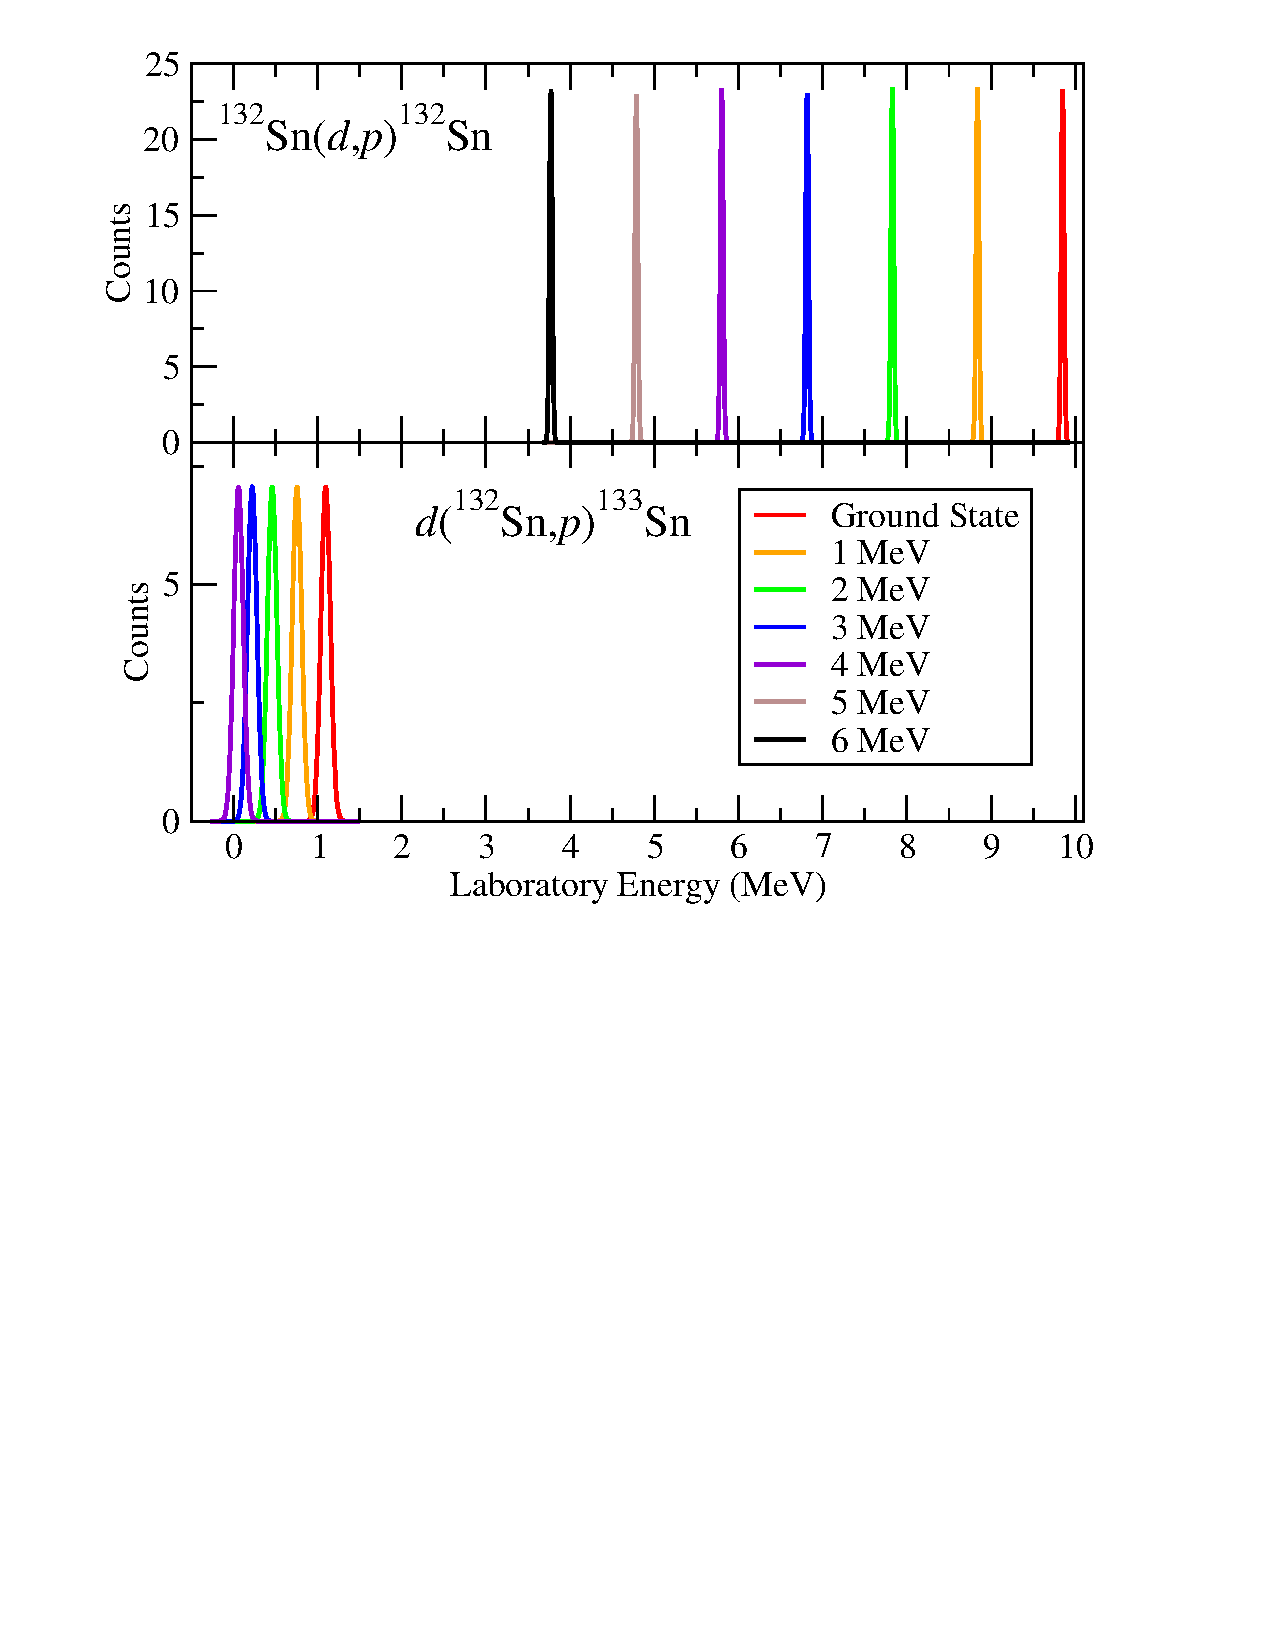
\includegraphics[width=\columnwidth,height=0.45\textheight,keepaspectratio]{sn132-plots4}
\caption[Illustration of the combined effect of kinematic compression and kinematic broadening]{Illustration of the combined effect of kinematic compression and kinematic broadening.  Calculated energy spectra are plotted for a fixed laboratory angle corresponding to at $\theta_\mathrm{cm}=10^\circ$, consistent with Fig.~\ref{sn-plots} and Table~\ref{error_prop}.  In normal kinematics (top, $\theta_\mathrm{lab}=9.9^\circ$), the energy level spacing approximately constant and equal to the spacing in the center-of-mass.  These states are plotted assuming an energy resolution of 40\,keV~FWHM.  In inverse kinematics (bottom, $\theta_\mathrm{lab}=149^\circ$), the energy spacing is dramatically compressed and the resolution is broadened to 133\,keV~FWHM.  States above $E_x > 5$\,MeV are not emitted in the rearward hemisphere.}%
\label{kin_broad_fig}%
\end{figure}

\subsection{Other Contributions}
\label{other_contrib}
\subsubsection{Intrinsic Width}
The discussion of resolution propagation presented above assumes that the states being measured have a natural width much smaller than the measurement uncertainty.  The intrinsic shape of an excited state is a Lorenzian distribution with a width given by the Heisenburg uncertainty principle
\begin{equation}
\Delta E \Delta t \leq \hbar
\label{eq:heisenburg}
\end{equation}
(here the standard symbol for uncertainty $\Delta$ has been used)\cite{Satchler_1990}.  If $\tau$ is the lifetime of the excited state, the width $\Gamma$ is given by 
\begin{equation}
\Gamma \simeq \hbar/\tau.
\label{eq:width}
\end{equation}
For example, the first-excited state in $^{29}$Si has a lifetime of $\tau=290$\,fs, which corresponds to a characteristic width of 2.3\,meV (\textit{milli}-electronvolts); this is a typical value for a bound nuclear excited state.  Therefore, under realistic conditions, the shape and width of measured excited states is dominated by the intrinsic detector resolution and, depending on the reaction, kinematic effects.  
In addition to the intrinsic resolution properties of the detector system, an important contribution to the $Q$-value resolution is the quality of the incident beam and the thickness of the target.

\subsubsection{Beam Energy}
The beam energy $E_1$ enters into the calculation of $E_\mathrm{cm}$ via the center-of-mass velocity $V_\mathrm{cm}$.  Rewriting $V_\mathrm{cm}$ in terms of $E_1$ yields
\begin{equation}
\begin{split}
V_\mathrm{cm}&=\sqrt{\frac{2E_1}{m_1}}\left(\frac{m_1}{m_1+m_2}\right).
\end{split}
\label{vcm2}
\end{equation}
Substituting this expression into Eq.~\ref{ecm3} and differentiating gives the contribution weight of the beam energy uncertainty $\delta E_1$ to the $Q$-value resolution.
\begin{equation}
\begin{split}
\frac{\partial E_\mathrm{cm}}{\partial E_1}&=\frac{m}{m_1}\left(\frac{m_1}{m_1+m_2}\right)^2-m(v_\mathrm{lab} \cos(\theta_\mathrm{lab}))\left(\frac{m_1}{m_1+m_2}\right)\sqrt{\frac{1}{2m_1E_1}}
\end{split}
\label{eq:delta_vcm}
\end{equation}
The value of $\delta E_1$ depends on many factors, such as method of beam production.  However, for an example with a stable beam, Fig.~\ref{beam_energy} shows  several measurements of the beam energy $E_1$ and the uncertainty in the beam energy $\delta E_1$ over the first five days of the  $d(^{28}\textrm{Si},p)^{29}\textrm{Si}$ experiment in Ref.~\cite{Lighthall_2010}.
The beam energy had a nominal value of 168\,MeV (6\,\AMeV) with a measured value of $E_1=168.53 \pm 0.24$\,MeV. %using the $\chi^2$ minimization method with $\delta E_1=\sigma_{E_1}=240$\,keV.
  This level of uncertainty corresponds to a relative uncertainty in the beam energy of $\delta E_1/E_1=0.14$\%.  The contribution of this uncertainty is shown in the sixth column of Table~\ref{error_prop}.  For unstable beams, the uncertainty in the beam energy will typically be higher than that for stable beams, although to what degree this is so depends on the method of beam production.

\begin{figure}[t]
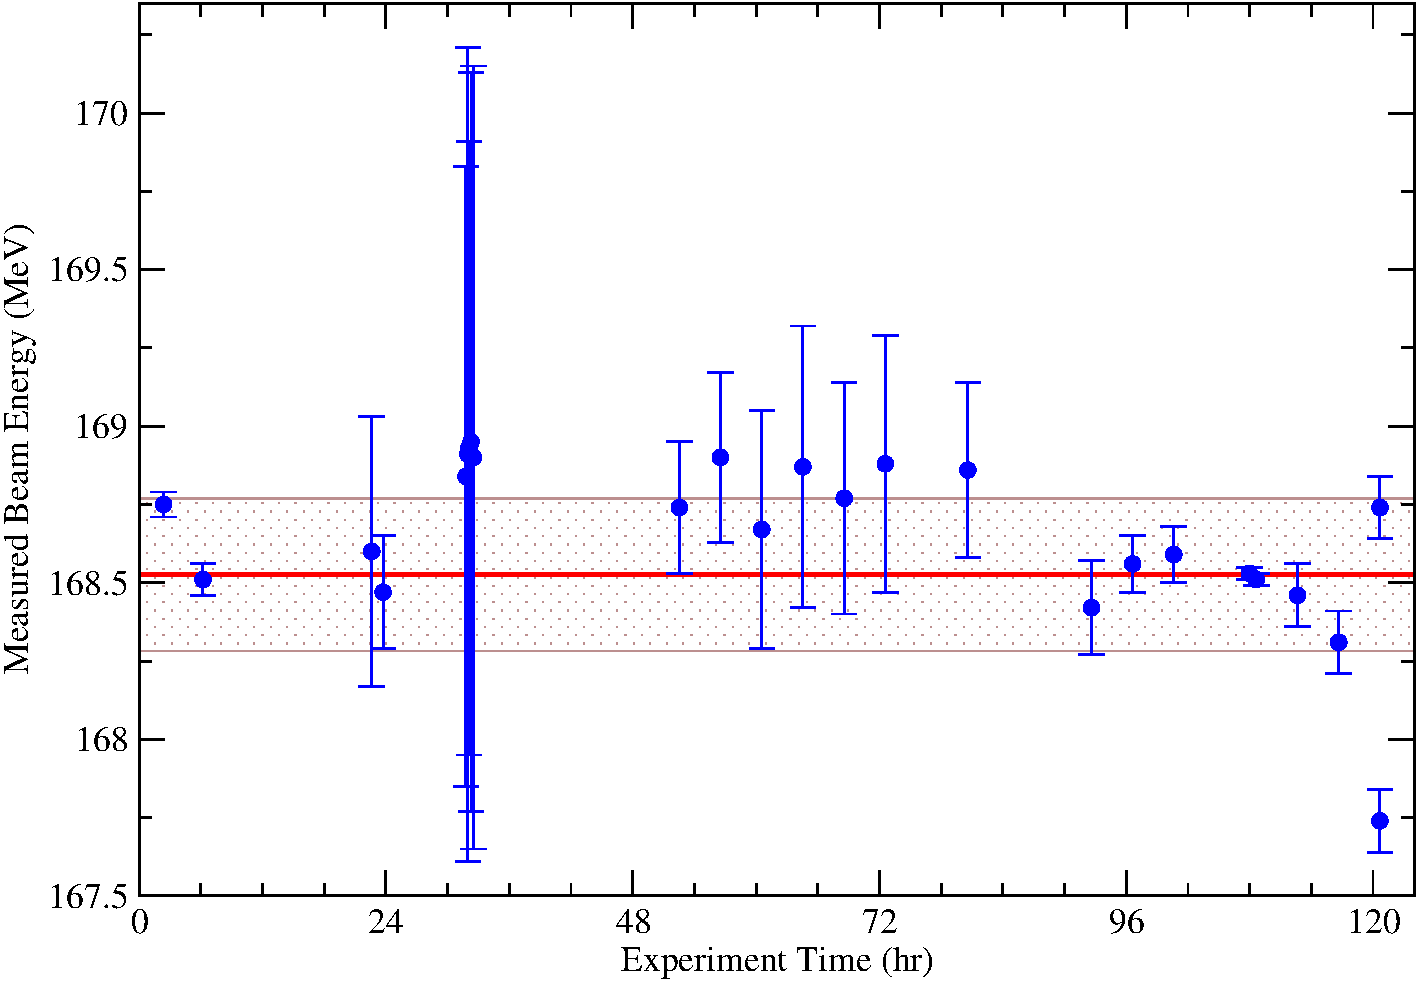
\includegraphics[width=\columnwidth]{beam_energy2}%
\caption[Beam energy and errors as measured during the $d$($^{28}$Si,$p$) experiment]{Beam energy and errors as measured during the $d$($^{28}$Si,$p$) experiment.  Both quantities measured by the ATLAS time-of-flight during the experiment reported in Ref.~\cite{Lighthall_2010}.  The horizontal line is the calculated average beam energy with $\pm 1 \sigma$ window.}%
\label{beam_energy}%
\end{figure}

\subsubsection{Beam Size}
Depending on the beam production technique, the heavy ion beam may have a substantial lateral extent---on the order of 1--5\,mm---at the target plane.  This transverse area is referred to as the beam spot size.  An increase in the uncertainty of the transverse extent of the interaction area between the beam and the target $\delta x$, $\delta y$ leads to a smearing of the measured scattering angle.  Fig.~\ref{beam_spot}(a) shows the effect of a finite beam spot size.  A similar effect, the effect of a misalignment of the beam, will also produce an error in determining the angle.  The contribution of this effect is discussed in Chapt.~\ref{simulation}.

\begin{figure}[t]%
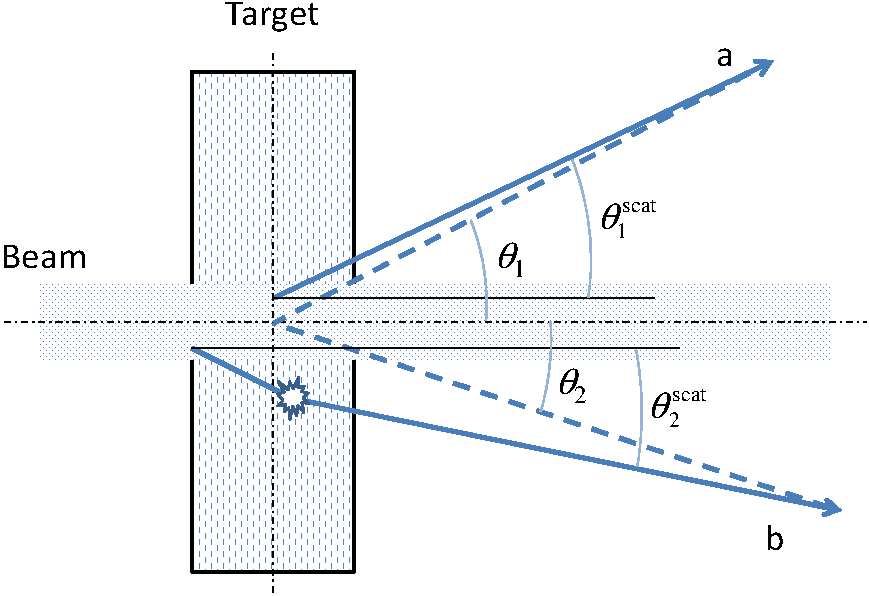
\includegraphics[keepaspectratio,width=\columnwidth,height=0.45\textheight]{beam_target}%
\caption[Illustration of the effect of beam spot size and target thickness on the light ejectile]{Illustration of the effect of beam spot size and target thickness on the light ejectile.  (a) The nuclear reaction occurs off the nominal beam axis, resulting in a disparity between the actual scattering angle $\theta_1^\textrm{scat}$ and the detected scattering angle $\theta_1$.  (b) The nuclear reaction occurs near the front of the target and the light ejectile scatters again while passing through the target.  Adapted from Ref.~\cite[Fig.~7]{Winfield_1997}}%
\label{beam_spot}%
\end{figure}

\subsubsection{Target Effects}
The light ions classically available for accelerated beams are not necessarily readily available, or perhaps practical, for use as target.  While most electrostatic accelerator facilities can produce pure beams of light ions, a solid cryogenic hydrogen target for high-resolution measurements, for instance, is impossible.  Instead, hydrogen beams are replaced with targets made of polyethylene (C$_2$H$_4$)$_{n}$ or polypropylene (C$_3$H$_6$)$_{n}$.  Similarly, the inverse kinematics analog of a deuteron beam could be a deuterated polyethylene (C$_2$D$_4$)$_{n}$ target.

The relatively low intensity beams achievable with most radioactive isotopes can be compensated for, in part, by the use of thicker targets.  However in a thicker target, the nuclear reactions can occur at a variety of depths.  When the bombarding beam consists of heavy ions, the energy loss associated with passing through the target $dE_1/dz$ (with $+z$ the direction of the beam) can be substantial.  For example, for a $^{132}$Sn beam incident on a 200\,$\mu$m thick (CD$_2$)$_{n}$ target will have an energy loss of about 15\,MeV.  In addition, as these effects vary randomly, the amount of energy loss that the beam experiences is not fixed, but has a finite distribution.  The spread in energy of the beam after passing through the target is known as energy straggling.  Finally, the collisions which lead to the energy loss also produce small angle scattering; this effect is known as multiple scattering.  Fig.~\ref{beam_spot}(b) illustrates the effect of a thick target on the light ion ejectile.  The target thickness effects of energy loss and multiple scattering impact the kinematics of both the incoming beam particle and the outgoing reaction products.  Due to the random nature of these effects, they are best treated using Monte Carlo simulation techniques.  This method is discussed in Chapt.~\ref{simulation}.  

%The contrary is also true.  For instance\note{Xe gas target\ldots HELIOS was the first device to measure the ($d$,$p$) reaction on $^{130}$Xe}
%\note{To compensate for the low intensity of radioactive beams, thicker targets may be used.  discussion of contributions to energy resolution, multiple scattering and energy loss}
%\include{Beams}
\chapter{Two Example Measurements}
\label{standards}
A successful measurement of a reaction in inverse kinematics requires a high-efficiency, high-resolution detector system with large acceptance and good background suppression.  The traditional solution to these issues is to use a large detector array with fine angular resolution~\cite{Pollacco_2005,Catford_2005,Demonchy_2007,Kanungo_2010}.  This chapter discusses two benchmark reaction measurements in inverse kinematics using the traditional---or non-solenoidal---detector approach wherein the laboratory energy $E_\mathrm{lab}$ of the detected particles is measured as a function of the laboratory angle $\theta_\mathrm{lab}$ to determine the center-of-mass quantities.

\section[\texorpdfstring{The $^\text{12}$B\lowercase{($d$,$p$)} Measurement}{The 12B(d,p) Measurement}]{\texorpdfstring{The $^\mathbf{12}$B($d$,$p$) Measurement}{The 12B(d,p) Measurement}}
\subsection{Introduction}
\label{b12intro}
A measurement of the $^{12}$B($d$,$p$) reaction was carried out at Argonne National Laboratory to study the neutron-rich $N=8$ nucleus $^{13}$B.  The details of this measurement are described in Ref.~\cite{Lee_2010}; this section summarizes those results.  Originally, the main purpose of this experiment was a nuclear structure study.  There is a pair of excited states in $^{13}$B near 3.6\,MeV, separated by 199\,keV, which had (at the time of the experiment) unknown spins. % and parities.
  The aim of this measurement was to resolve this doublet and through the analysis of the resulting angular distributions, determine the angular momentum transfer $\ell_n$ and assign spins and parities $J^\pi$ to the states.

\subsection{Experimental Setup}
%\section{Ludwig's Castle}
The experiment was carried out in the scattering chamber upstream from the Enge Split-Pole Spectrograph in ATLAS Target Area III (SPSIII), referred to internally as Ludwig's Castle.  
\subsubsection{Beam Production}
\label{beamprod}
$^{12}$B is unstable against $\beta$-decay with a half-life of $T_{1/2}=20.2$\,ms.  Therefore, a reaction involving $^{12}$B must be performed in inverse kinematics.  In this example, the $^{12}$B beam is produced in-flight, following the method %of beam production used in this experiment
which is described in detail in Ref.~\cite{Harss_2000}.  A primary beam of stable $^{11}$B ions at an energy of 81\,MeV and an intensity of 100\,pnA bombarded a cryogenic gas cell to produce the secondary radioactive beam. % via the $d$($^{12}$B,$p$) reaction.
The production cell is shown in Fig.~\ref{gas_cell}.  The gas cell was filled with D$_2$ deuterium gas at a pressure of 1400\,mbar and temperature of $-185$\,$^\circ$C to produce a target with an areal density of 1.6\,mg/cm$^2$.  The secondary $^{12}$B beam was produced in the neutron transfer reaction $d$($^{11}$B,$^{12}$B)$p$.  The resulting radioactive beam bombarded an 150\,$\mu$g/cm$^2$ target of deuterated polyethylene (C$_2$D$_4$)$_n$ with an average beam intensity of $1.2\times 10^5$\,ions/s.

\begin{figure}%
\centering
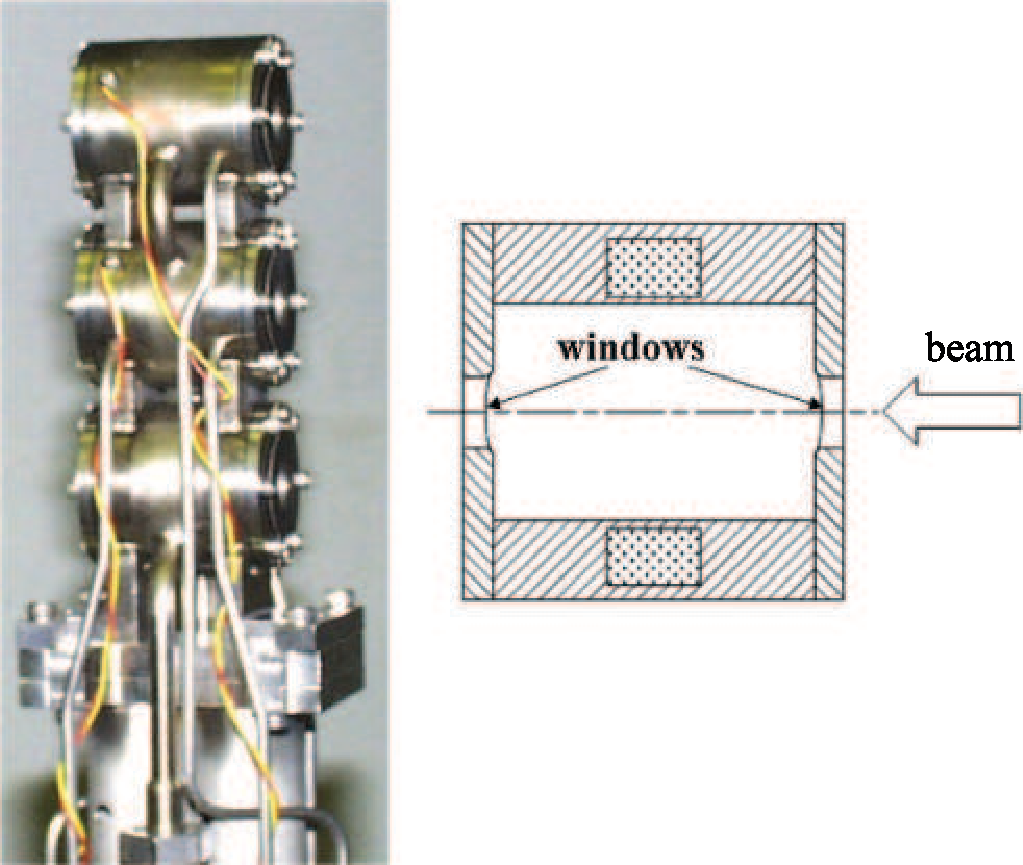
\includegraphics[height=0.5\textwidth,width=\columnwidth,keepaspectratio]{GastargetFig2}%
\caption[Gas cell used for in-flight beam production at ATLAS]{Gas cell used for in-flight beam production at ATLAS.  The type of gas cell used to produce the radioactive $^{12}$B beam in-flight are 3.7\,cm long and 2.54\,cm in diameter. Havar$\textsuperscript{\textregistered}$ foils 1.9\,mg/cm$^2$ thick serve as windows on the entrance and exit of the gas cell.}
\label{gas_cell}%
\end{figure}

\subsubsection{Detectors}
The  detector setup for measuring transfer reactions within Ludwig's Castle is described in Ref.~\cite{Wuosmaa_2005}.  The same basic setup was used in this measurement.  The detector array utilized in this experiment consists of three 500\,$\mu$m thick double-sided silicon strip detectors (DSSD) of design S1 manufactured by Micron Semiconductor.  The annular detectors have an inner radius of 24\,mm and an outer radius of 48\,mm, for a total active area of 53\,cm$^2$.  One side of each detector is segmented into 16 concentric rings of $\Delta r=1.5$\,mm, while the other side is segmented into 16 wedges, each covering $\Delta \phi =22.5^\circ$; thus each detector requires 32 electronics channels.  To suppress spurious counts, a detector signal is required in an element on both sides of a given detector in order to be included in the trigger logic.  Heavy recoils are identified downstream from the target in a $\Delta E$-$E$ detector array discussed in Chapt.~\ref{recoil}.  In an adjacent scattering chamber downstream from the heavy recoil detectors, a surface barrier detector is placed in the beam path behind an % 100$\times$
 attenuator to monitor the beam current.

Fig.~\ref{annular_dets} shows the physical relationship of the detectors to the target foil within the scattering chamber.  The  $^{12}$B($d$,$p$) reaction has a $K_\mathrm{g.s.}$-value of 0.61, which means forward angles in the center-of-mass correspond to rearward angles in the laboratory ($\theta_\mathrm{lab}>90^\circ$); hence the detector array is position upstream from the target foil.  Table~\ref{coverage} shows the solid-angle coverage for the detector array.  The entire array covered a solid angle of 1.10\,sr.

\begin{figure}%
\centering
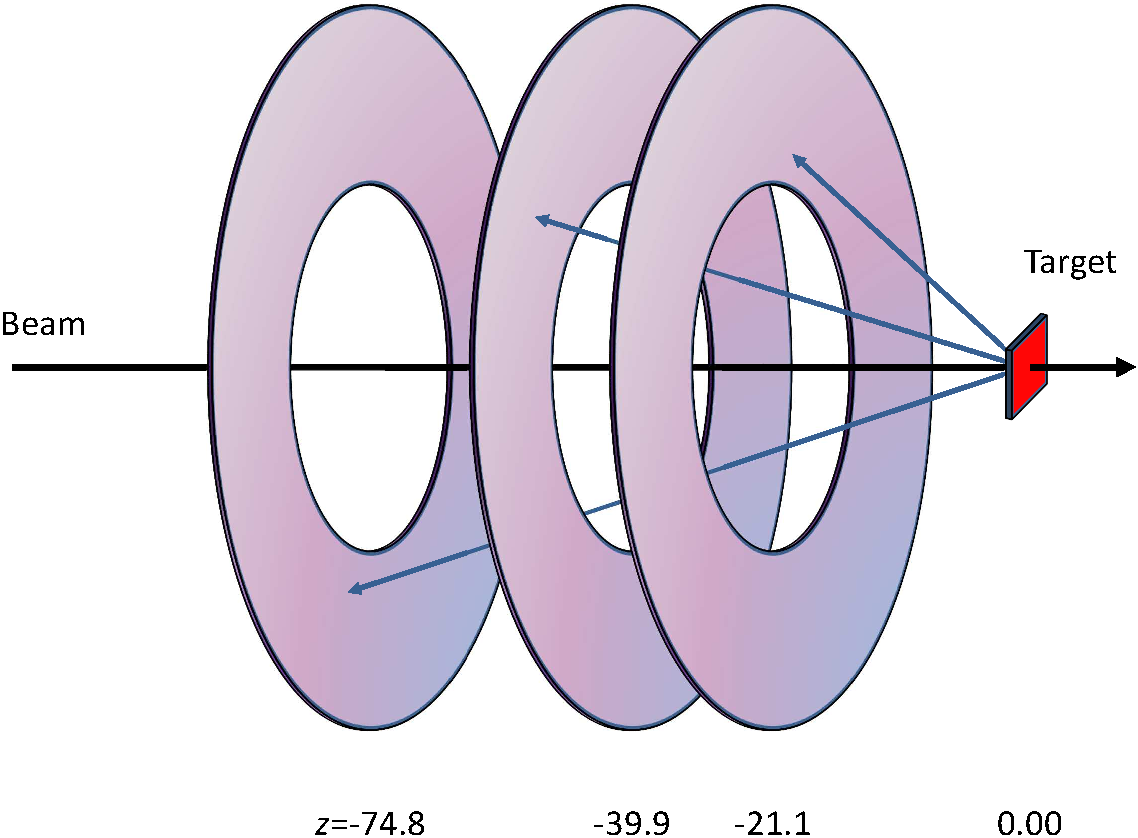
\includegraphics[width=\columnwidth,height=0.33\textheight,keepaspectratio]{annular}%
\caption[Detector setup for the $^{12}$B($d$,$p$) measurement in inverse kinematics]{Detector setup for the $^{12}$B($d$,$p$) measurement in inverse kinematics (drawn to scale).  Protons ejected in the rearward hemisphere ($\theta_\mathrm{lab}>90^\circ$) are detected by three annular detectors covering $114^\circ<\theta_\mathrm{lab}<162^\circ$.  }%
\label{annular_dets}%
\end{figure}

\begin{table}%
\centering
\begin{tabular}{ccrrcrrcc}
\hline
Det.&$z$&\multicolumn{2}{c}{$\theta_\mathrm{lab}$}&&\multicolumn{2}{c}{$\theta_\mathrm{cm}$}&$\Delta \cos(\theta_\mathrm{cm})$&$\Delta \Omega$\\ \cline{3-4} \cline{6-7}
&(mm)&\multicolumn{1}{c}{$\theta_1$}&\multicolumn{1}{c}{$\theta_2$}&&\multicolumn{1}{c}{$\theta_1$}&\multicolumn{1}{c}{$\theta_2$}&&(sr)\\
\hline \hline
1&$-21.1$&113.7&131.3&&32.4 &21.5 & 0.086  & 0.54\\
2&$-39.9$&121.9&141.2&&27.0 &16.4 & 0.068  & 0.43\\
3&$-74.8$&147.3&162.2&&13.5 &7.1 & 0.020  & 0.13\\
  \multicolumn{7}{r}{Total} &0.175&1.10\\
 \hline
\end{tabular}
\caption[Detector positions and solid angle coverage for the $^{12}$B($d$,$p$) measurement]{Detector positions and solid angle coverage for the $^{12}$B($d$,$p$) measurement.  Protons ejected in the rearward hemisphere ($\theta_\mathrm{lab}>90^\circ$) are detected by three annular detectors covering $114^\circ<\theta_\mathrm{lab}<162^\circ$.  }
\label{coverage}
\end{table}

\subsection{Results}
\begin{figure}%
\centering
\hspace*{\stretch{1}}%
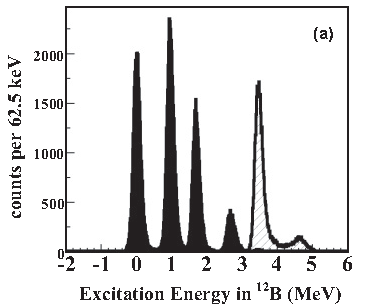
\includegraphics[width=0.45\textwidth,height=0.33\textheight,keepaspectratio]{Lee_2010_fig1b}\hspace*{\stretch{1}}
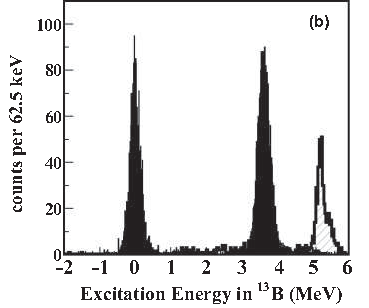
\includegraphics[width=0.45\textwidth,height=0.33\textheight,keepaspectratio]{Lee_2010_fig1d}\hspace*{\stretch{1}}
\caption[Excitation energy spectra from the $^{11,12}$B($d$,$p$) reactions in inverse kinematics]{Excitation energy spectra from the $^{11,12}$B($d$,$p$) reactions in inverse kinematics.  The energy resolution is 250\,keV.  The black peaks in both spectra correspond states populated in the residual nucleus which lie below the neutron-decay threshold; 3.4\,MeV for $^{12}$B and 4.9\,MeV for $^{13}$B.  The white (hatched) peaks correspond to states which are neutron-unbound.  (a) In the $^{11}$B($d$,$p$) spectrum, the $\Delta E_x=102$\,keV doublet near 2.7\,MeV is unresolved.  (b) In the $^{12}$B($d$,$p$) spectrum, the $\Delta E_x=199$\,keV doublet near 3.6\,MeV is unresolved.  Figure from Ref.~\cite[Fig.~1]{Lee_2010}.}
\label{b11b12_spec}%
\end{figure}

As shown in Table~\ref{error_prop}, the expected energy resolution of the $^{12}$B($d$,$p$) reaction is on the order of 120\,keV.  This estimate neglects beam spot size ($\approx 3$\,mm ) and target thickness (150\,$\mu$g/cm$^2$) effects. The beam spot size will have the same effect on any measurement.  The target thickness, however, has a pronounced effect on the $Q$-value resolution in inverse kinematics because the heavy ion experiences significant energy loss entering and exiting the target. %The beam spot size was 
Therefore, the reported $Q$-value resolution of 250\,keV is not surprising.  However, this resolution was insufficient to resolve the states at $E_x=3.482$ and 3.681\,MeV ($\Delta E_x=199$\,keV).  Therefore the separate angular distributions of these states could not be analyzed, making a determination of the angular momentum transfer impossible.  Fig.~\ref{b11b12_spec} shows the excitation energy spectra for both reactions.  The measurement of this reaction was re\-at\-tempt\-ed in order to separate these states using the HELIOS spectrometer as discussed in Chapt.~\ref{rib_com}.

Although %the $Q$-value resolution of this measurement was insufficient to separate the doublet near 3.6\,MeV, 
the original aim of this experiment was not realized,
the experiment did provide a new measurement that had astrophysical implications.  Eq.~\ref{eq:a12rproc} shows the $r$-process path through the light elements.  Included in the reaction chain is neutron capture on $^{11}$B (indicated by the underbrace).  The $^{11}$B($d$,$p$)$^{12}B$ neutron-transfer reaction is an example of a measurement that can be used to study the $r$-process.  Recoil tagging, using particle identification in the $\Delta E$-$E$ array (discussed in Chapt.~\ref{recoil}), was used to measure the branching ratio of $^{12}$B decay.  The neutron-unbound 3.389\,MeV state in $^{12}$B is predominately populated in coincidence with the recoiling $^{12}$B nucleus, corresponding to $\gamma$-decay of $^{12}$B$^\textrm{*}$.  However, a fraction of the events populating the 3.389\,MeV state were measured in coincidence with a $^{11}$B, corresponding to in-flight $n$-decay.   The ratio of the yield of these events is related to resonant neutron capture in $^{11}$B which contributes to both the overall rate of the $r$-process~\cite{Surman_2009}.  The details of this relationship are discussed in Ref.~\cite{Lee_2010}.

\begin{equation}
^{1}\textrm{H}(n,\gamma)^{2}\textrm{H}(n,\gamma)^{3}\textrm{H}(d,n)^{4}\textrm{He}(t,\gamma)^{7}\textrm{Li}(n,\gamma)^{8}\textrm{Li}(\alpha,n)\underbrace{^{11}\textrm{B}(n,\gamma)^{12}\textrm{B}}(\beta^-)^{12}\textrm{C}(n,\gamma)^{13}\textrm{C}
\label{eq:a12rproc}
\end{equation}


\section[\texorpdfstring{The $^\text{132}$S\lowercase{n($d$,$p$)} Measurement}{The 132Sn(d,p) Measurement}]{\texorpdfstring{The $^\mathbf{132}$Sn($d$,$p$) Measurement}{The 132Sn(d,p) Measurement}}
\subsection{Introduction}
%\section{ORRUBA}
A sophisticated example of a large acceptance array with excellent resolution is the Oak Ridge Rutgers university Barrel Array (ORRUBA) in concert with the  Silicon Detector Array (SIDAR) at the Holifield Radioactive Ion Beam Facility (HRIBF) at Oak Ridge National Laboratory.  This detector array was used to study the ($d$,$p$) neutron transfer reaction on the neutron-rich, doubly-magic ($N=82$, $Z=50$) nucleus $^{132}$Sn.  The results of this measurement are reported in Refs.~\cite{Jones_2007,Pain_2008,Jones_2010}; this section summarizes those results.

\subsection{Experimental Setup}
%\subsubsection{Beam Production}
A $^{132}$Sn beam was produced using the isotope separation online (ISOL) technique.  The $^{132}$Sn ions were created as fission fragments from protons bombarding a uranium carbide target.  The $^{132}$Sn fission fragments were re-accelerated with the HRIBF 25\,MeV tandem Van de Graaff accelerator to an energy of 4.78\,\AMeV, producing an essentially pure beam.  %The resultant beam had an intensity of $2\times10^5$\,ions/s.
A 100\,$\mu$g/cm$^2$ CD$_2$ target was used, rotated 60$^\circ$ to the beam axis for an effective thickness of 160\,$\mu$g/cm$^2$.  The target was rotated to allow particles emitted near $\theta_\mathrm{lab}=90^\circ$ to be detected.

%\subsubsection{Detectors}
\begin{figure}%
\centering
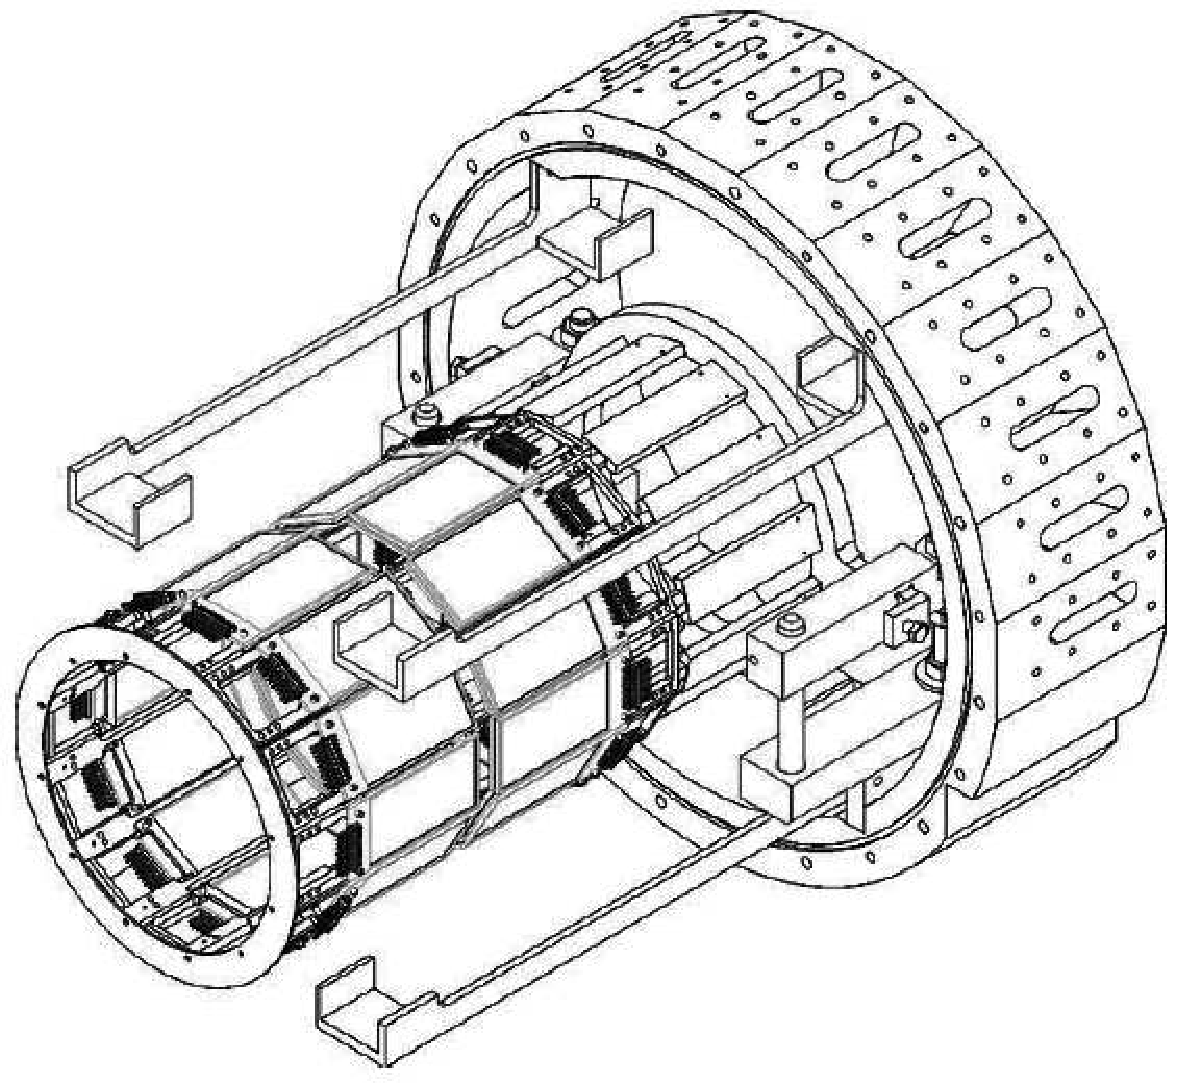
\includegraphics[width=\columnwidth,height=0.33\textheight,keepaspectratio]{Pain_2007-fig2}%
\caption[Engineering schematic of the ORRUBA detector system]{Engineering schematic of the ORRUBA detector system.  Beam enters from left.  In addition to showing two rings of detectors separated by a small gap, this figure also includes cable trays, the detector support structure and the preamplifier feedthrough ring.  Figure enhanced from Ref.~\cite{Pain_2007}.}%
\label{orruba}%
\end{figure}

The ORRUBA detector array, shown in Fig.~\ref{orruba}, is specifically designed to meet the challenges of measuring inverse kinematics: it has a large spacial coverage and is capable of making high resolution measurements of both energy and angle.  The details of the detector array construction are discussed in Ref.~\cite{Pain_2007}.  The ORRUBA detector array essentially consists of two rings of detectors positioned forwards and  backwards of $\theta_\mathrm{lab}=90^\circ$.  For the d($^{132}$Sn,p)$^{133}$Sn measurement, the upstream ring of detectors consisted of single-layer position sensitive detectors; the downstream ring was made up of $\Delta E$-$E$ telescopes, with the residual $E$ detectors also being position sensitive.  In this configuration, the detector array provides angular resolution of $<0.5^\circ$, position resolution of 0.5\,mm~FWHM, and (intrinsic) energy resolution of $<60$\,keV~FWHM.  Fig.~\ref{133Sn_e_spec_sim} shows a simulated spectrum of the d($^{132}$Sn,p)$^{133}$Sn based on these parameters.  The results of the simulation are in agreement with the analytic calculations of Fig.~\ref{sn-plots}.

\begin{figure*}
\begin{center}
\centering
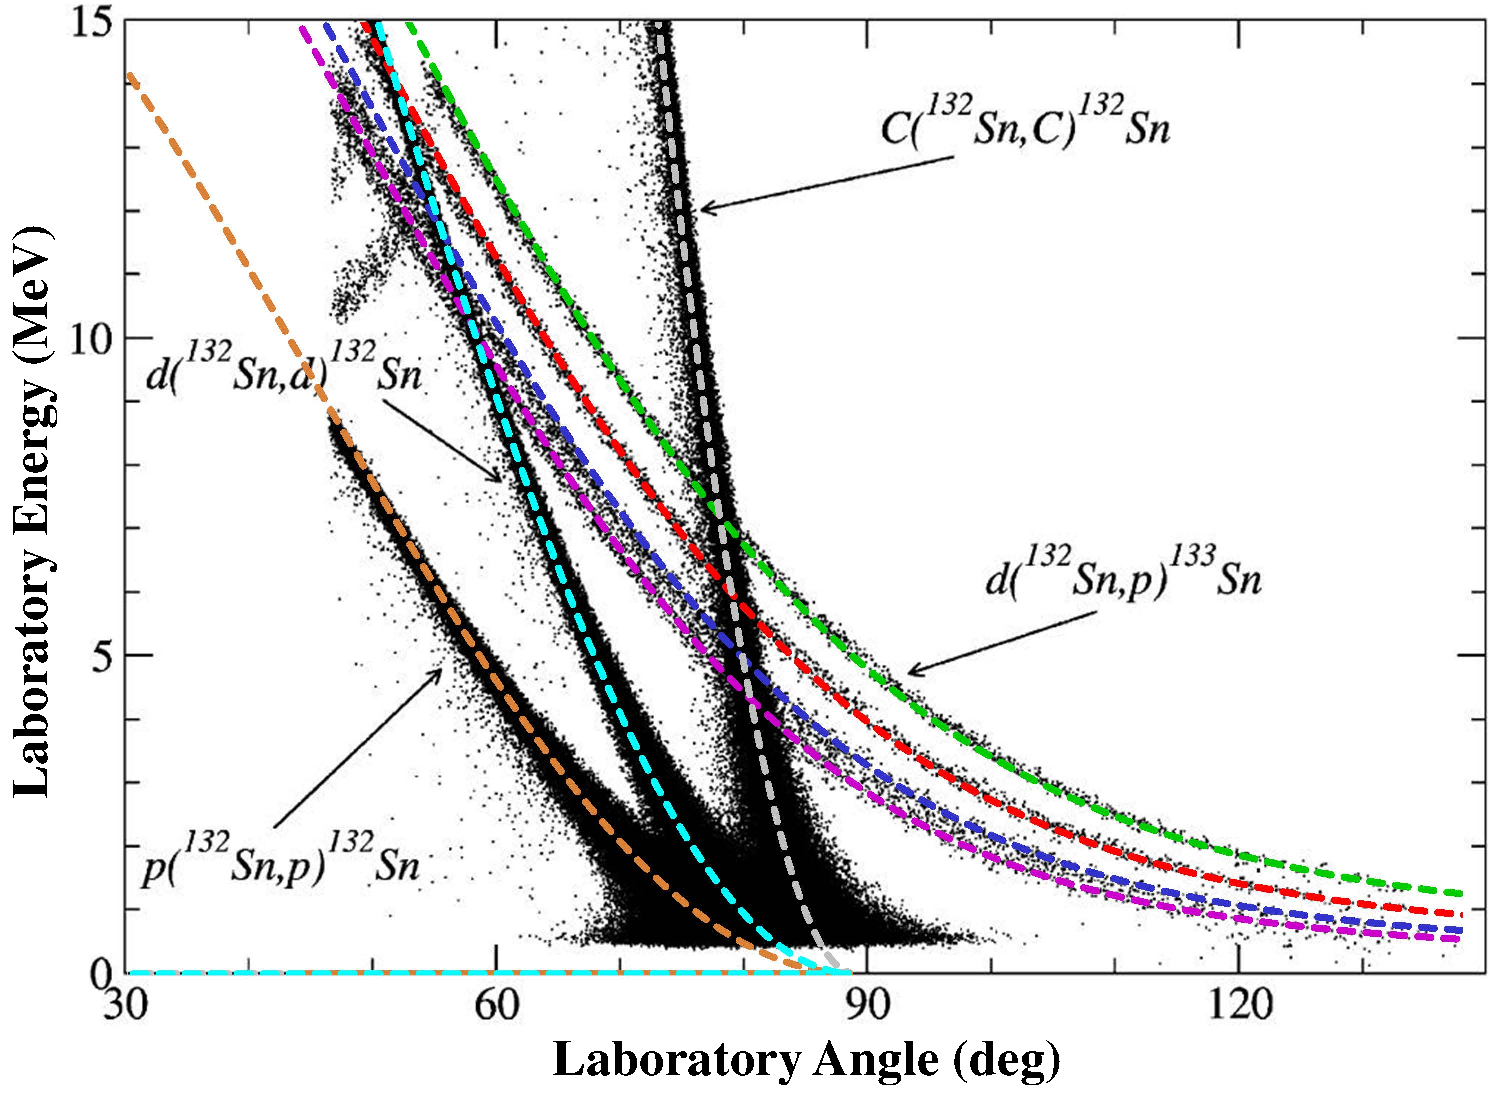
\includegraphics[keepaspectratio,height=0.3\textheight]{Pain_2007-fig1an-6}
\end{center}
\caption[Simulated $E_\mathrm{lab}$ vs. $\theta_\mathrm{lab}$ spectrum for the $d$($^{132}$Sn,$p$)$^{133}$Sn  reaction at 4.78\,\AMeV with ORRUBA]{(color online) Simulated $E_\mathrm{lab}$ vs. $\theta_\mathrm{lab}$ spectrum for the $d$($^{132}$Sn,$p$)$^{133}$Sn reaction at 4.78\,\AMeV with ORRUBA. The simulation includes elastic scattering of protons, deuterons, and $^{12}$C.  Analytical calculations have been plotted over the simulated results using the axes of the original figure.  The calculations are color-coded to match Fig.~\ref{133Sn_e}.  At $\theta_\mathrm{lab}=120^\circ$ 
  ($\theta_\mathrm{cm}=22.9^\circ$) the kinematic compression coefficient  is $\Delta E_\mathrm{lab}/\Delta E_\mathrm{cm}=0.34$.  Annotated    figure taken from Ref.~\cite{Pain_2007}.}
\label{133Sn_e_spec_sim}%
\end{figure*}

\subsection{Results}
\label{orrubaresults}
The ground-state and three excited states at $E_x=0.845$, 1.363, and 2005\,MeV were identified in this measurement. The state at $E_x=1.363\pm0.031$\,MeV was previously unobserved.  The $E_\mathrm{lab}$ versus $\theta_\mathrm{lab}$ proton spectrum produced is shown in Fig.~\ref{133Sn_e_spec}.  The analytic calculations of Fig.~\ref{sn-plots} have been plotted over the data (with re-calculated excitation energies).  Table~\ref{error_prop} shows that, neglecting target thickness effects, the $Q$-value resolution should be, at best, 133\,keV~FWHM.  Fig.~\ref{133Sn_e} shows the measured $Q$-value spectrum which has an energy resolution of over 300\,keV~FWHM.  Angular distributions were measured for the two lowest levels.  The ground state showed $\ell_n=3$ character, consistent with the $2f_{7/2}$ assignment; and the first-excited state at $E_x=0.845$ had an angular distribution characteristic of an $\ell_n=1$ transfer, corresponding to the $3p_{3/2}$ orbital.

\begin{figure*}
\begin{center}
\centering
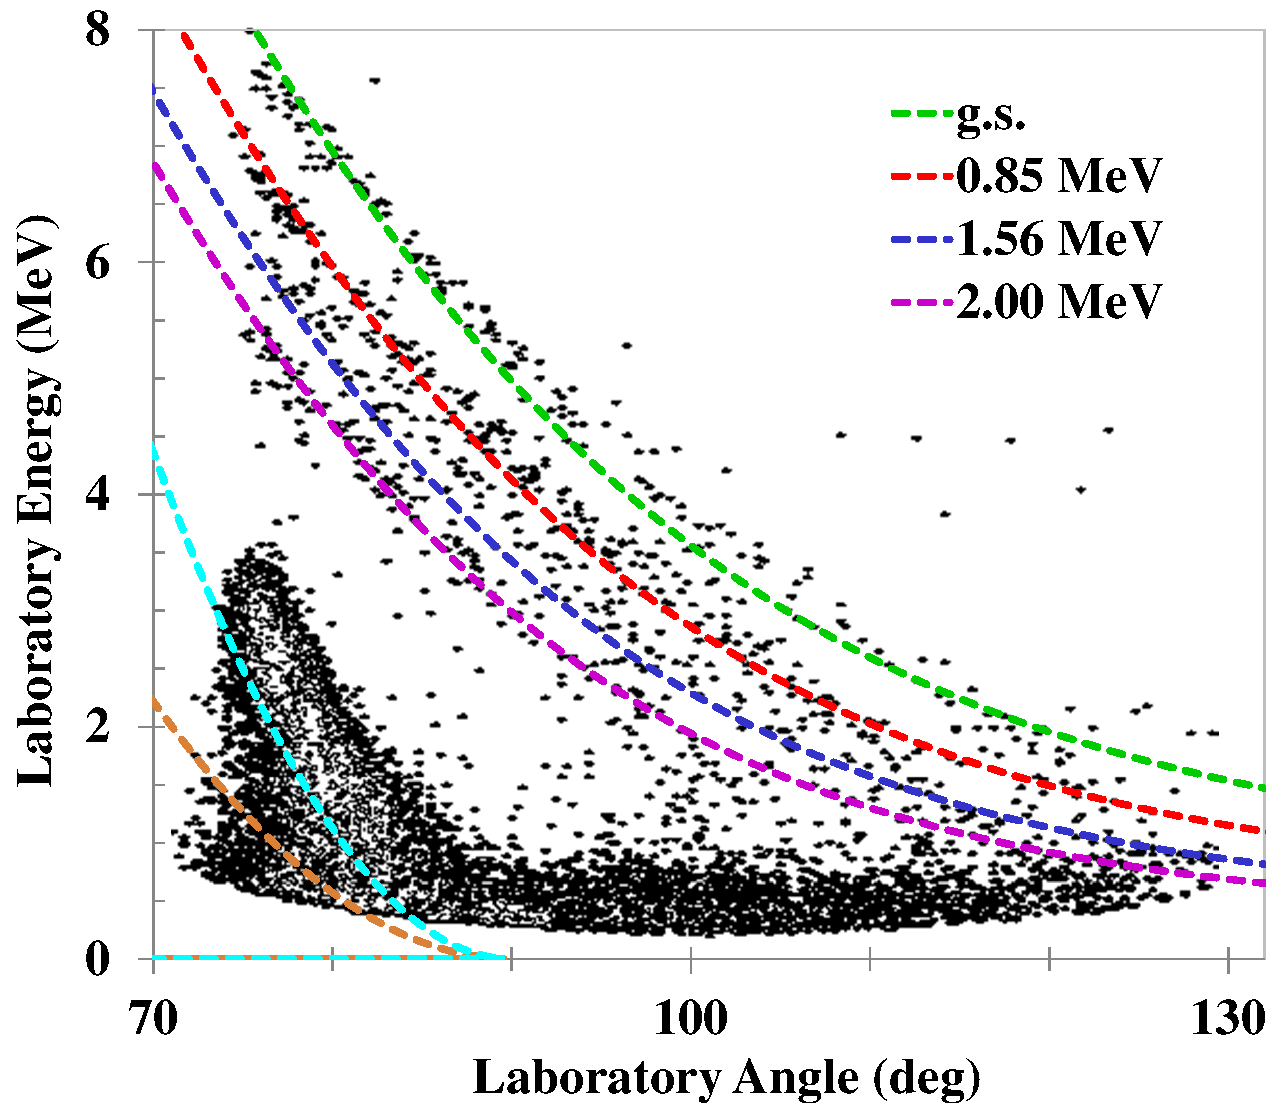
\includegraphics[keepaspectratio,height=0.3\textheight]{Jones_2007-2b}
\end{center}
\caption[Measured $E_\mathrm{lab}$ vs. $\theta_\mathrm{lab}$ spectrum for the $d$($^{132}$Sn,$p$)$^{133}$Sn reaction at 4.78\,\AMeV with ORRUBA]{(color online) Measured $E_\mathrm{lab}$ vs. $\theta_\mathrm{lab}$ spectrum for the $d$($^{132}$Sn,$p$)$^{133}$Sn reaction at 4.78\,\AMeV with ORRUBA.   Analytical calculations have been (roughly) plotted over the results, showing good agreement.  The axes of the calculations plot are shown.  Annotated figure taken from Ref.~\cite{Jones_2007}.}%
\label{133Sn_e_spec}%
\end{figure*}
%\subsection{Discussion}
Other reports are available in the literature of neutron transfer reactions in the $A=130$ region using ORRUBA.  An early proof-of-concept experiment was carried out using the lampshade SIDAR array and a prototypical form of the ORRUBA array to study the $^{124}$Sn($d$,$p$) reaction in inverse kinematics~\cite{Jones_2004}.  This measurement had a reported $Q$-value resolution of 200\,keV~FWHM.  %Using this set-up, the study was successful in producing a center-of-mass energy spectrum and the associated angular distributions.  Since then, 
Additional ($d$,$p$) studies have been carried out using %a more-complete form of 
the ORRUBA detector and other neutron-rich isotopes---$^{131}$Sn~\cite{Kozub_2008} and $^{134}$Te~\cite{Pain_2008}---both have excitation energy spectra with resolution on the order of 200--300\,keV~FWHM.  This collection of results provide a consistent description of the performance characteristics of this detector array.  In order to improve on the results obtained with ORRUBA, a detector system is needed which can avoid or suppress the effects of resolution degradation due to the covariance of measured quantities (kinematic broadening).

\begin{figure}[hb!]
\begin{center}
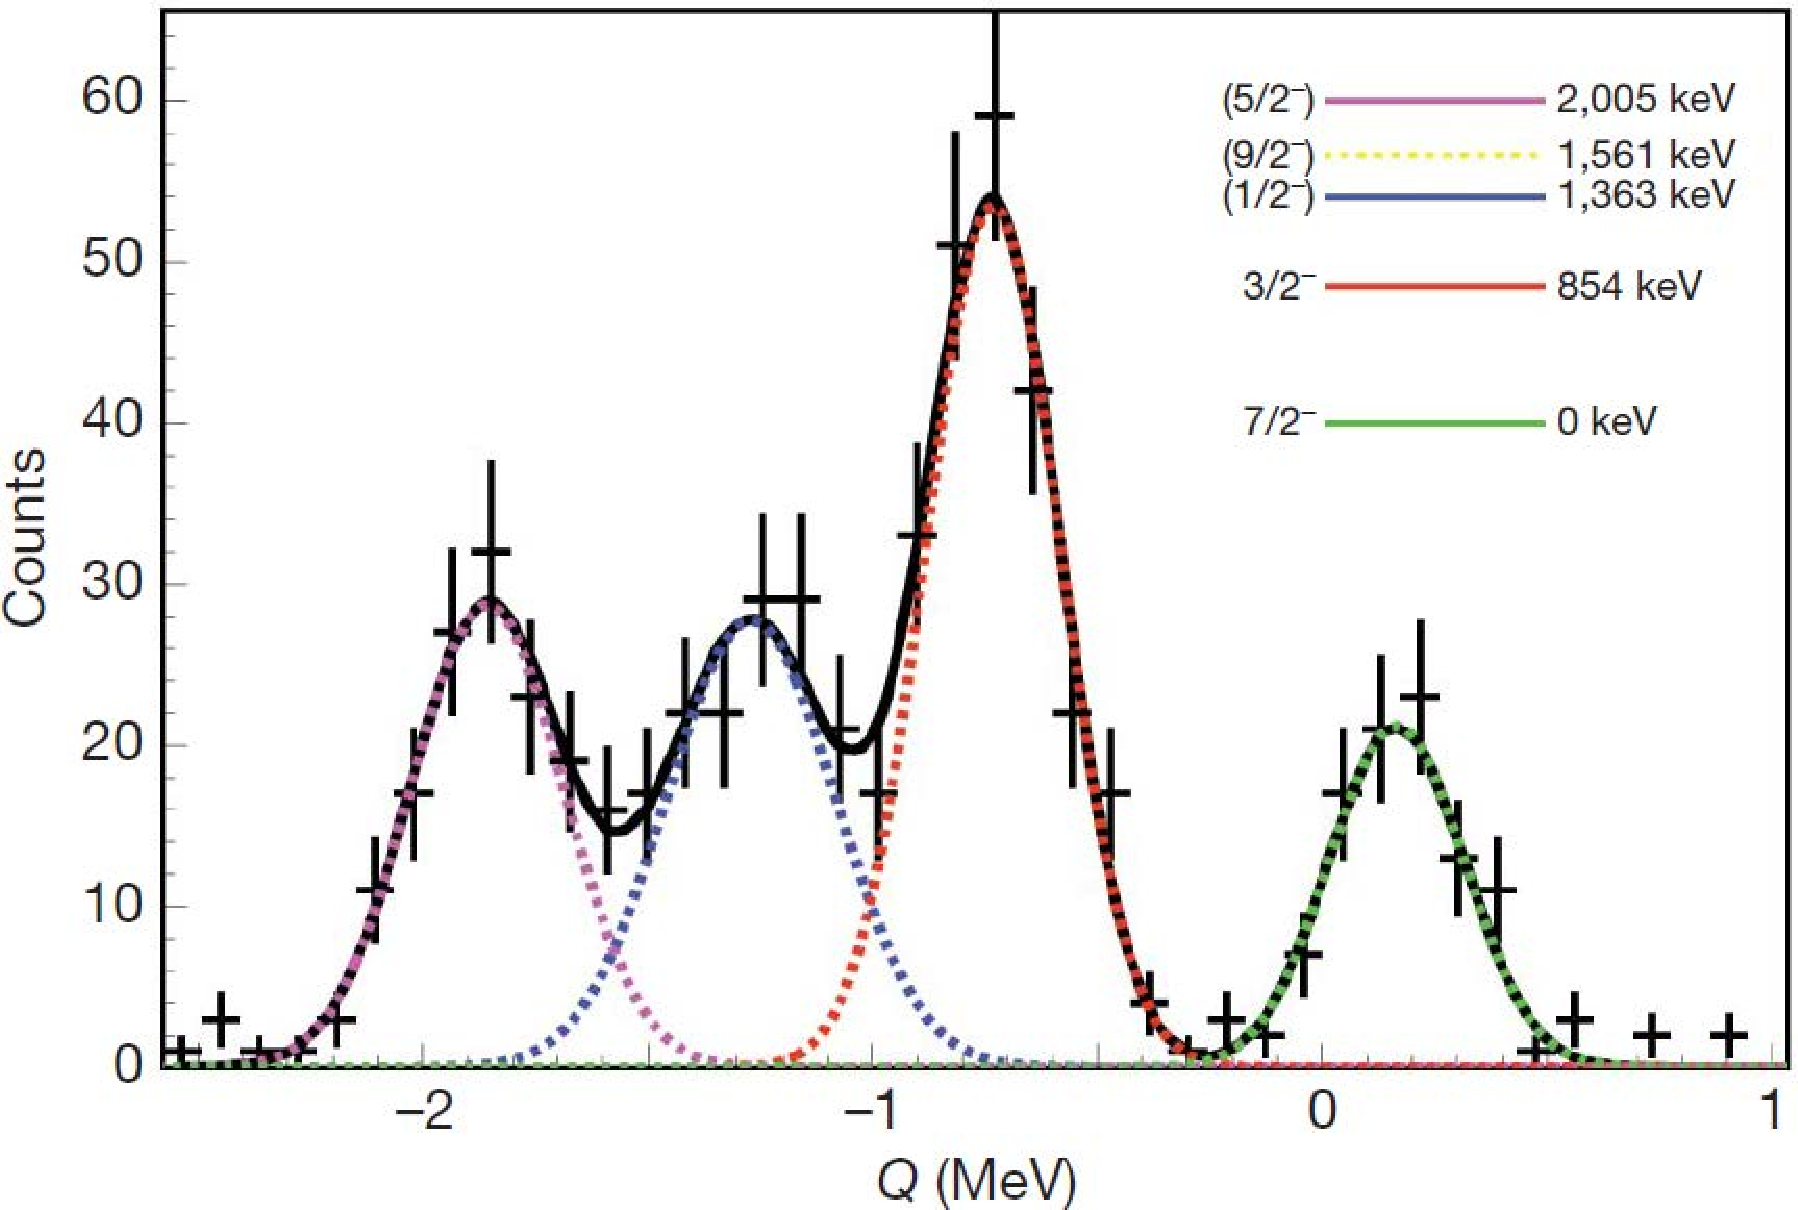
\includegraphics[keepaspectratio,width=\columnwidth,height=0.3\textheight]{Jones_2010-fig2-j}
\end{center}
\caption[$Q$-value spectrum from the $d$($^{132}$Sn,$p$)$^{133}$Sn reaction at 4.78\,\AMeV with ORRUBA]{(color online) $Q$-value spectrum from the $d$($^{132}$Sn,$p$)$^{133}$Sn reaction at 4.78\,\AMeV with ORRUBA.  Measured at $\theta_\mathrm{cm}=54^\circ$.  The $Q$-value resolution is 300\,keV~FWHM.  Figure taken from Ref.~\cite{Jones_2010}.}%
\label{133Sn_e}%
\end{figure}
\chapter{The HELIOS Concept}
\label{HELIOS_Concept}
%The HELIOS spectrometer is specifically designed to address the challenges encountered in inverse kinematics. 
The HELIcal Orbit Spectrometer (HELIOS) offers a new way of studying reactions in inverse kinematics that has several advantages over the detection methods mentioned in Chapt.~\ref{standards}.  The conceptual principle of HELIOS is introduced in Refs.~\cite{Schiffer_1998,Schiffer_2003}; the proposed design and performance characteristics are laid out in Refs.~\cite{Wuosmaa_2003,Wuosmaa_2007}, and the technical realization and the details of the experimental commissioning are presented in Ref.~\cite{Lighthall_2010}.  The goal of this chapter is to summarize, derive, and expand on the key mathematical concepts presented in these references.
\begin{figure}[!ht]
\centering
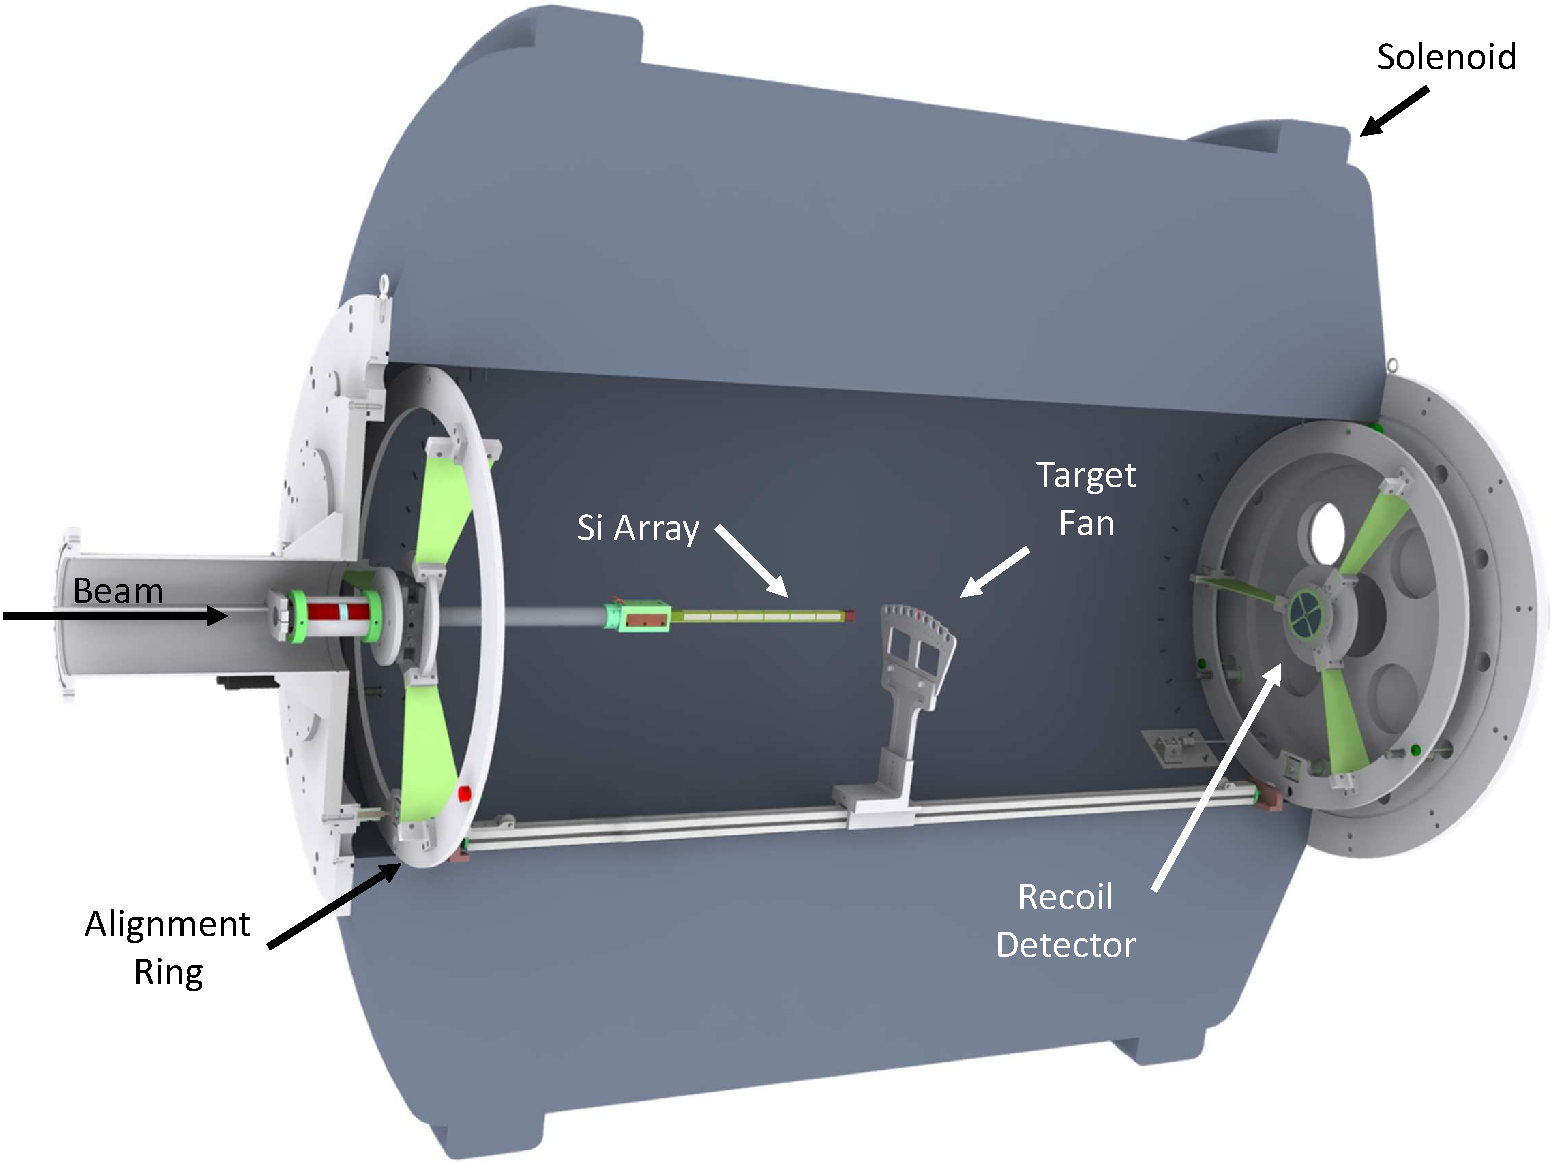
\includegraphics[width=\linewidth,height=0.5\textheight,keepaspectratio]{NIM_Paper/Figures/18pt_rot3}
\caption[Cutaway schematic view of HELIOS in the ``($d$,$p$)'' configuration]{Cutaway schematic view of HELIOS in the ``($d$,$p$)'' configuration.  The accelerated beam enters from left.  Shown are the light-ion silicon detector array suspended on the upstream alignment ring, rotating target fan, and heavy-recoil detector.  Mechanical design by S.~Heimsath.  3D rendering by B.~J.\ DiGiovine.  This figure also appears in Ref.~\cite{Lighthall_2010}.}
\label{schematic}
\end{figure}

Schematically, HELIOS is based on a large-bore superconducting solenoid, as shown in an engineering model in Fig.~\ref{schematic}.  Accelerated heavy-ion beams enter the solenoid along the magnetic axis, passing through a hollow detector array.  The beam then intercepts a ``light-ion'' target, also on the magnetic axis.  In the configuration shown in the figure, charged reaction products ejected rearward in the laboratory frame---that is, $\theta_\mathrm{lab}>90^\circ$---move in helical orbits to the detector array.  Beam-like recoils are kinematically focused forward in a narrow cone and intercepted by a detector array for identifying heavy ions.
\section{Solenoid Kinematics}
\label{solkin}
The solenoid used in HELIOS produces what is effectively an uniform axial magnetic field.  The technical specifications of the solenoid as well as the features of the magnetic field are discussed in detail in Chapt.~\ref{sol}.  When a reaction occurs within such a magnetic field, the trajectories of the reaction products are simplified due to the constraints of cyclotron motion.  With the solenoid axis aligned collinearly with the beam axis, ions emitted at the target travel in helical orbits under the influence of the magnetic field and return to the magnetic field axis.
\subsection{Coordinates}
\label{coord}
The particle trajectories are defined by the orientation of the laboratory velocity $\vec{v}_\mathrm{lab}$ relative to the solenoid axis.  The symmetry of the solenoid defines a cylindrical coordinate system ($z$,$\rho$,$\phi$), with the beam traveling in the $+z$ direction and the azimuthal angle $\phi=0$ defined relative to ``beam right'' (the $+x$ axis).  Furthermore, the coordinate convention used with HELIOS defines the $+y$ axis as ``up'' yielding a left-handed coordinate system.  With this convention in mind, the laboratory velocity may be written as 
\begin{equation}
\vec{v}_\mathrm{lab}=v_\parallel \hat{z}+v_\perp \hat{\rho}
\label{lab_vel}
\end{equation}
with $v_\parallel$ and $v_\perp$ defined in terms of the polar angle as
\begin{equation}
\begin{split}
v_\perp&\equiv v_\mathrm{lab}\sin(\theta_\mathrm{lab})\\
&=v_0\sin(\theta_\mathrm{cm})\\
\end{split}
\end{equation}
and
\begin{equation}
\begin{split}
v_\parallel &\equiv v_\mathrm{lab}\cos(\theta_\mathrm{lab})\\
&=V_\mathrm{cm}+v_0\cos(\theta_\mathrm{cm})\\
\end{split}
\label{eq:vpara}
\end{equation}
 as illustrated in Fig.~\ref{vector}.  In these equations $v_0$ retains its definition from Eq.~\ref{kin_v0}.
\begin{figure}
\begin{center}
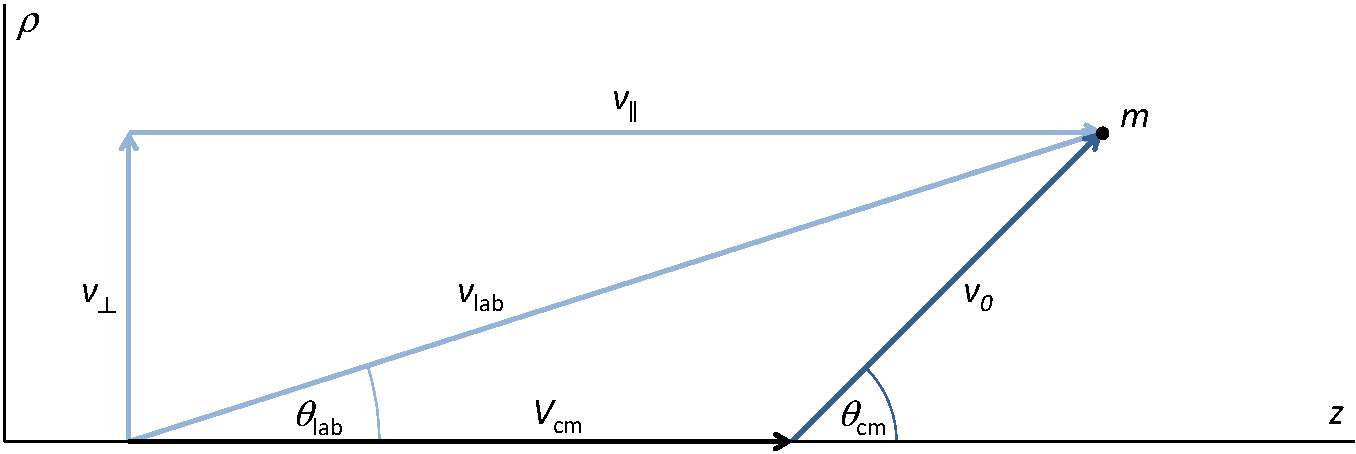
\includegraphics[width=\columnwidth]{kin_fig_4c}
\setlength{\unitlength}{0.125\columnwidth}
%\fbox{
%\begin{picture}(4.5,2.75)(.25,.125)
%\thinlines
%\put(0.5,0.50){\line(1,0){3.75}}%z
%\put(0.5,0.50){\line(0,1){2}}   %rho
%\thicklines
%\put(1,0.5){\vector(1,0){2}}    %Vcm
%\put(1,0.5){\vector(3,2){3}}    %vlab
%\put(3,0.5){\vector(1,2){1}}    %v0

%\put(2,0.3){$V_\mathrm{cm}$}
%\put(2,1.5){$v_\mathrm{lab}$}
%\put(3.65,1.5){$v_0$}
%\put(1.4,0.6){$\theta_\mathrm{lab}$}
%\put(3.2,0.6){$\theta_\mathrm{cm}$}
%\put(4.4,0.45){$z$}
%\put(.45,2.7){$\rho$}
%\end{picture}
%}%end fbox
\end{center}
\caption[Vector diagram of relevant velocities of the mass $m$ ejectile]{Vector diagram of relevant velocities of the mass $m$ ejectile. $\vec{v_\mathrm{lab}}=\vec{V_\mathrm{cm}}+\vec{v_0}$ with $v_\mathrm{lab}$ the ejectile velocity in the laboratory, $V_\mathrm{cm}$ the velocity of the center-of-mass, and $v_0$ the ejectile velocity in the center-of-mass.  The velocity projections $v_\perp$ and $v_\parallel$ are defined as illustrated.}%
\label{vector}%
\end{figure}
\subsection{Cyclotron Motion}
The velocity component perpendicular to the solenoid axis $v_\perp$ defines the radius of cyclotron motion 
\begin{equation}
\begin{split}
r=v_{\perp}\frac{m}{\mathscr{B}q}\\
\end{split}
\label{cyc_rad}
\end{equation}
for a particle of mass $m$ and charge $q$ traveling in a field of strength $\mathscr{B}$.  A related quantity, the cyclotron period $T_\mathrm{cyc}$, is fixed by the mass-to-charge ratio of the particle and the magnetic field strength. 
\begin{equation}
\begin{split}
T_\mathrm{cyc}&=\frac{2\pi r}{v_{\perp}}\\
       &=\frac{2\pi}{\mathscr{B}} \left(\frac{m}{q}\right)
\end{split}
\label{Tcyc}
\end{equation}
\par The position at which particles return to the solenoid axis varies according to their velocity parallel to the magnetic field $v_\parallel$.  As such, HELIOS disperses ions by $v_\parallel$.  For a given value of $(m/q)$ and magnetic field, the axial path length (return distance) is given by
\begin{equation}
\begin{split}
z_n&=v_\parallel (n \times  T_\mathrm{cyc})
\end{split}
\label{loops}
\end{equation}
after executing $n$ number of orbits.  For purposes of nomenclatural clarity, it is useful at this point to introduce the variable $z_1$, the point at which a particle undergoing a single orbit intercepts the solenoid axis.

\section{Determining the Center-of-mass Quantities}
Particles are detected within HELIOS along the length of a hollow array of position sensitive silicon detectors (PSDs) suspended on the solenoid axis.  This detector arrangement represents a fundamental departure from the tradition measurement approach wherein the scattering angle $\theta_\mathrm{lab}$ is measured.  When a light ion intercepts an active portion of the silicon detector array, three quantities are measured: the energy $E$, the time of flight $t$, and the axial position $z$.    From these measured quantities, the 
center-of-mass quantities of energy $E_\mathrm{cm}$ and emission angle $\theta_\mathrm{cm}$ are derived.  
\subsection{Excitation Energy}
The transformation of the energy of the ejectile in the laboratory frame to the energy in the center-of-mass frame can be reduced to a linear transformation.  Substituting Eq.~\ref{eq:vpara} into Eq.~\ref{elab}, the laboratory energy $E_\mathrm{lab}$ can be rewritten as
%Starting with %the non-relativistic definition of kinetic energy, $E_\mathrm{lab}=\frac{1}{2} m(v_\mathrm{lab})^2$, %the equations of \S\,\ref{coord} can be used to rewrite 

\begin{equation}
\begin{split}
%E_\mathrm{lab}&=%\frac{1}{2} m(v_\parallel^2+v_\perp^2 )\\
%&=\frac{1}{2} m\left[(V_\mathrm{cm} +v_0 \cos(\theta_\mathrm{cm}))^2+v_0^2 \sin^2(\theta_\mathrm{cm})\right]\\
%&=\frac{1}{2} m\left[V_\mathrm{cm}^2 +2V_\mathrm{cm}v_0 \cos(\theta_\mathrm{cm})+v_0^2\cos^2(\theta_\mathrm{cm})+v_0^2 \sin^2(\theta_\mathrm{cm})\right]\\
%\frac{1}{2} m\left[v_0^2+V_\mathrm{cm}^2 +2V_\mathrm{cm}v_0 \cos(\theta_\mathrm{cm})+\right]\\
E_\mathrm{lab}&=\frac{1}{2} m\left[v_0^2+V_\mathrm{cm}^2 +2V_\mathrm{cm}v_0 \cos(\theta_\mathrm{cm})\right]\\
&=\frac{1}{2} m\left\{v_0^2+2V_\mathrm{cm}[v_0 \cos(\theta_\mathrm{cm})+V_\mathrm{cm}-V_\mathrm{cm}]+V_\mathrm{cm}^2 \right\}\\
%&=\frac{1}{2} m\left[V_\mathrm{cm}^2 +2V_\mathrm{cm}v_\parallel-2V_\mathrm{cm}^2+v_0^2\right]\\
&=\frac{1}{2} m\left(v_0^2+2V_\mathrm{cm}v_\parallel -V_\mathrm{cm}^2\right).
\end{split}
\label{elab_of_vpara}
\end{equation}

A given beam energy fixes the value of $V_\mathrm{cm}$ and, given a reaction and transition, $v_{0}$ is fixed.  Therefore, the measured energy $E_\mathrm{lab}$ depends linearly according to $v_\parallel$, the laboratory velocity parallel to the beam axis.  Assuming the particles are detected on the magnetic axis, this quantity has a value of $v_\parallel=z_n/(n T_\mathrm{cyc})$.  Inserting this expression into Eq.~\ref{elab} and   rearranging to solve for the center-of-mass energy, defined as $E_\mathrm{cm}=\frac{1}{2}m( v_0)^2$, gives the center-of-mass energy as a linear offset from the laboratory energy. 
\begin{equation}
E_\mathrm{cm}=E_\mathrm{lab}+\frac{1}{2} mV_\mathrm{cm}^2-\frac{m V_\mathrm{cm}}{n T_\mathrm{cyc}}z_n
\label{ecm}
\end{equation}
%Measuring the position of axis intercept relative to the target, combined with the fixed time-of-flight, disperses particles , their   The position of axis intercept $z$, together with the measured laboratory energy, defines the center-of-mass angle and energy of the reaction in a linear relationship
The excitation energy $E_x$ is then derived from the center-of-mass energy by correcting for the recoil mass of the residual nucleus. Substituting Eq.~\ref{eq:ecm} into Eq.~\ref{eq:ecmtotal} and solving for $E_x$ yields
\begin{equation}
E_x=T_\mathrm{cm}+Q-E_\mathrm{cm}\frac{m+M}{M}
\label{eq:recoil_mass}
\end{equation}

\subsection{Emission Angle}
In order to study the angular distributions for transitions to different excited states, it is necessary to calculate the scattering angle in the center-of-mass $\theta_\mathrm{cm}$.  With reference to Fig.~\ref{vector}, the center-of-mass angle is readily obtained using the law of cosines.
%Equation moved to kinematics chapter.

Starting with the %velocity relation given by the low of cosines in 
Eq.~\ref{eq:law_of_cosines} and solving for $\theta_\mathrm{cm}$ yields
\begin{equation}
\begin{split}
\theta_\mathrm{cm}=&\arccos\left(\frac{v_\mathrm{lab}^2-v_0^2-V_\mathrm{cm}^2}{2v_0 V_\mathrm{cm}}\right).
%\theta_\mathrm{cm}=&\arccos\left[\frac{\frac{2}{m}(E_\mathrm{lab}-E_\mathrm{cm})-V_\mathrm{cm}^2}{\sqrt{2 E_\mathrm{cm}/m}V_\mathrm{cm}}\right]
\end{split}
\label{costhetacm}
\end{equation}
This is the familiar result of two-body kinematics from classical mechanics (\textit{cf}.~\citet[Eq.~3.109]{Goldstein_2002}).
As alluded to earlier, $V_\mathrm{cm}$ is fixed by the bombarding energy of the beam.  Once the excitation energy is determined using Eq.\,\ref{ecm}, the value of $v_0$ is fixed.  Thus, for a given transition, the center-of-mass angle is uniquely determined by $v_\mathrm{lab}$, which is calculated from the measured laboratory energy $E_\mathrm{lab}$.  

\section{Advantages}
The principles laid out in this chapter describing the HELIOS concept provide a number of advantages over traditional detection techniques.
\subsection{Particle Identification}
\par The cyclotron period is an especially important quantity because it defines the time of flight for the detected particles and provides particle identification.  The time-of-flight is approximately%ed by 
\begin{equation}
T_\mathrm{cyc}=65.1\,\textrm{ns}\times \frac{An}{q\mathscr{B}}
\end{equation}
with $A$ the atomic mass number, $n$ is the number of orbits, $q$ in units of $e$, and $\mathscr{B}$ in Tesla.  Table~\ref{flight_times} gives the cyclotron periods ($n=1$) for the H and He isotopes with $A\leq 4$ for %$\mathscr{B}=2.0$\,T.
a variety of field strengths.  The minimum separation in ns of the cyclotron periods for these light ions is approximately  $32.6/\mathscr{B}$, where $\mathscr{B}$ is in units of T.  With a field strength of $\mathscr{B}=2.0$\,T, this separation is 16.3\,ns; timing resolution of this magnitude is readily achievable with typical silicon detectors.  Thus, by means of measuring the time of flight, HELIOS solves the problem of particle identification of light-ion reaction products at low energy.  The particle identification is valid up to ambiguities of $An/q$.
\begin{table}
  \begin{center}
    \begin{tabular}{cccc}
      \hline
      \multicolumn{1}{c}{\multirow{2}{*}{Ion}}  &
    	\multicolumn{3}{c}{$T_\mathrm{cyc}$ (ns)}\\ \cline{2-4}
    	%&$q\mathscr{B}/n=1$\,e$\cdot$T&2\,e$\cdot$T&3\,e$\cdot$T\\\hline \hline 
    	&$\mathscr{B}/n=1$\,T&2\,T&3\,T\\\hline \hline 
      $p$&65.6&32.8&21.9\\
      $^3$He&98.2&49.1&32.7\\
      $\alpha$&130.3&65.2&43.4\\
      $d$&131.2&65.6&43.7\\
      $t$&196.4&98.2&65.5\\\hline
    \end{tabular}
    \label{flight_times}
    \caption[Cyclotron periods $T_\mathrm{cyc}$ for typical reaction products for a variety of field strengths]{Cyclotron periods $T_\mathrm{cyc}$ for typical reaction products for a variety of field strengths.}
  \end{center}
\end{table}
\subsection{\texorpdfstring{$Q$-value Resolution}{Q-value Resolution}}
The most significant feature of the HELIOS concept is that it avoids the problem of kinematic compression introduced in \S\,\ref{kin_comp}.  Instead of detecting ions %over a range of 
at fixed laboratory angles, the ions transported by the magnetic field within HELIOS are %measured over a range of 
detected at 
fixed axial positions.  Eq.~\ref{ecm} gives a linear relationship between the measured quantities $E_\mathrm{lab}$ and $z$ and the derived quantity $E_\mathrm{cm}$.  This linear relationship between the laboratory quantities and the center-of-mass system is the key to the enhanced $Q$-value resolution of HELIOS.  Table~\ref{helios_error} shows the calculated $Q$-value resolution for a number of reactions based on the HELIOS concept.  Following the discussion in \S\,\ref{res_prop}, the contributions are calculated assuming energy measurement uncertainties of $\delta E_\mathrm{lab}=40$\,keV~FWHM, and an uncertainty in the beam energy of 0.14\%. In addition, the contribution from the uncertainty of the position is based on $\delta z=1.0$\,mm~FWHM.  As can be seen in the table, the dominant contribution to the $Q$-value resolution is the intrinsic detector resolution, as was the case in normal kinematics.

\begin{table*}%
  \centering
  \begin{tabular}{,......rr}		
    \hline
    \multicolumn{1}{c}{\multirow{2}{*}{Reaction}}  &
    \multicolumn{1}{c}{$E_1/A_1$}  &
    \multicolumn{1}{c}{$\mathscr{B}$}  &
    \multicolumn{1}{c}{$\theta_\textrm{lab}$} & 
    \multicolumn{3}{c}{Origin of contribution}  &
    \multicolumn{2}{c}{$\delta E_\textrm{cm}$}  \\  \cline{5-7}
    &\multicolumn{1}{c}{(\AMeV)}&
    \multicolumn{1}{c}{(T)}&
    \multicolumn{1}{c}{(deg)} & 
    \multicolumn{1}{c}{$\delta z$}  &  
    \multicolumn{1}{c}{$\delta E_\textrm{lab}$} & 
    \multicolumn{1}{c}{$\delta E_1$} & 
    \multicolumn{1}{c}{$\Sigma_\mathrm{quad}$} &
    \multicolumn{1}{c}{$\Sigma_\mathrm{covar}$} \\
    \hline \hline 
    d(^{28}\textrm{Si},p)^{29}\textrm{Si} 	& 6.02 & 2.00 & 157.9 &11 & 40 & 13 & 43 & 32\\
    d(^{12}\textrm{B},p)^{13}\textrm{B} 	 &6.24 & 1.04 & 155.2 &5 & 40 & 11 & 42 & 37\\
    d(^{132}\textrm{Sn},p)^{133}\textrm{Sn}	 &4.78 & 2.00 & 149.0 &10 & 40 & 10 & 42 & 31\\
    d(^{124}\textrm{Sn},^3\textrm{He})^{123}\textrm{In} 	 &13.00 & 2.73 & 21.5 &45 & 40 & 38 & 71 & 38\\
    p(^{77}\textrm{Kr},d)^{76}\textrm{Kr}  	 &30.00 & 2.00 & 15.1 &24 & 40 & 51 & 70 & 54\\
    \hline
  \end{tabular}
  \caption[Calculated contributions to the uncertainty of $E_\textrm{cm}$ for measurements using HELIOS]{Calculated contributions to the uncertainty of $E_\textrm{cm}$ for measurements using HELIOS.  For experiments that have already been preformed, the actual magnetic field value is used; for experiments that have not been run---$^{132}$Sn and $^{77}$Kr---a 2.00\,T field is assumed.  Values are calculated in keV~FWHM for $\theta_\mathrm{cm} = 10^\circ$.  The quadratic sum $\Sigma_\mathrm{quad}$ and the sum including the covariant term $\Sigma_\mathrm{covar}$ are given.}
  \label{helios_error}
\end{table*}

\subsubsection{Energy Separation}
\label{energysep}
At a fixed $z$ position, kinematic loci are separated %, by definition,
 by their laboratory energy $\Delta E_\mathrm{lab}=(E_\mathrm{lab}-E_\mathrm{lab}^\prime)$.  This quantity is related to the center-of-mass energy separation by
\begin{equation}
\begin{split}
\Delta E_\mathrm{lab}%&=\left[E_\mathrm{cm}-\frac{1}{2} mV_\mathrm{cm}^2+\frac{m V_\mathrm{cm}}{T_\mathrm{cyc}}z_1\right]_1-\left[E_\mathrm{cm}-\frac{1}{2} mV_\mathrm{cm}^2+\frac{m V_\mathrm{cm}}{T_\mathrm{cyc}}z_1\right]_2\\
&=\left[E_\mathrm{cm}-\frac{1}{2} mV_\mathrm{cm}^2+\frac{m V_\mathrm{cm}}{T_\mathrm{cyc}}z_1\right]-\left[E_\mathrm{cm}^\prime-\frac{1}{2} mV_\mathrm{cm}^2+\frac{m V_\mathrm{cm}}{T_\mathrm{cyc}}z_1^\prime\right]%\\
%&=\Delta E_\mathrm{cm}
\end{split}
\label{eq:delta_e}
\end{equation}
in which the second term in the bracketed expressions is constant for a given bombarding energy and the last term is constant for fixed $z$.  Taking the difference, these terms drop out and we are left with
\begin{equation}
\Delta E_\mathrm{lab}=\Delta E_\mathrm{cm}.
\label{eq:no_comp}
\end{equation}
Comparing this expression to Eq.~\ref{eq:compress}, on sees the ``compression'' coefficient leading the $\Delta E_\mathrm{cm}$ term is identically equal to $1$ and is independent of scattering angle.  Hence, the separation between kinematic groups corresponding to different energy levels in the residual nucleus at a fixed $z$ is the same as the energy spacing in the center-of-mass frame.  Put another way, with measurements made with HELIOS, there is no kinematic compression. 
This result arises from the constant slope of the kinematic loci, given by
\begin{equation}
\begin{split}
\frac{\partial E_\mathrm{lab}}{\partial z}&=\frac{m V_\mathrm{cm}}{nT_\mathrm{cyc}}
\end{split}
\label{slopeEcm}
\end{equation}
which is independent of $z$ and the reaction $Q$-value and hence is free from kinematic compression. Substituting Eqs.~\ref{Vcm} and \ref{Tcyc} into this expression one also sees the slope is independent of the ejectile mass $m$.
\begin{equation}
\begin{split}
\frac{\partial E_\mathrm{lab}}{\partial z}&=\frac{q\mathscr{B}}{2\pi n}\sqrt{\frac{2 E_1}{m_1}}\left(\frac{m_1}{m_1+m_2}\right)\\
&\approx 2.21\,\textrm{keV/mm} \times \frac{q \mathscr{B}}{n}\sqrt{\frac{E_1}{A_1}}\left(\frac{A_1}{A_1+A_2}\right)
\end{split}
\label{slope_calc}
\end{equation}
where $A_1$ and $A_2$ are the atomic mass numbers of the beam and the target nuclei, respectively; $q$ in units of $e$, and $\mathscr{B}$ in Tesla.  In the limit of inverse kinematics $m_1\gg m_2$, the term in the parentheses is equal to one.  Table~\ref{slopes} gives slopes for the H and He isotopes for a number of field strengths and bombarding energies.

\begin{table}
  \begin{center}
    \begin{tabular}{........}
      \hline
      \multicolumn{1}{c}{$E_1/A_1$(\AMeV)}%&$\mathscr{B}=1$\,T&2\,T&3\,T\\\hline \hline %\\[-2ex]
      &\multicolumn{7}{c}{$q\mathscr{B}/n$ (e$\cdot$T)}\\ \cline{2-8}
      &\multicolumn{1}{c}{0.5}
      &\multicolumn{1}{c}{1.0}
      &\multicolumn{1}{c}{1.5}
      &\multicolumn{1}{c}{2.0}
      &\multicolumn{1}{c}{3.0}
      &\multicolumn{1}{c}{4.0}
      &\multicolumn{1}{c}{6.0}\\\hline \hline 
%      5&4.9& 9.8&14.7\\
%      10&6.9&13.9&20.8\\
%      15&8.5&17.0&25.5\\
%      20&9.8&19.6&29.4\\
			5  & 2.4 & 4.9 &  7.3 &  9.8 & 14.7 & 19.6 & 29.4 \\
			10 & 3.5 & 6.9 & 10.4 & 13.8 & 20.8 & 27.7 & 41.5 \\
			15 & 4.2 & 8.5 & 12.7 & 17.0 & 25.4 & 33.9 & 50.9 \\
			20 & 4.9 & 9.8 & 14.7 & 19.6 & 29.4 & 39.2 & 58.7 \\ \hline
    \end{tabular}
    \label{slopes}
    \caption[Typical slopes of $E_\mathrm{lab}$ vs. $z$ with HELIOS]{Typical slopes of $E_\mathrm{lab}$ vs. $z$ with HELIOS.  Values are given in keV/mm for various bombarding energies and parameter values $q=1$, 2\,e; $\mathscr{B}=1$, 2, 3\,T; and $n=1$,2.}
  \end{center}
\end{table}

The effect of kinematic compression as exhibited by 
%This effect in 
HELIOS
%, or rather, the lack thereof 
is illustrated in Fig.~\ref{helios_basic}.   In practice, this effect is utilized by correcting for the slope of the kinematic curves by means of Eq.~\ref{ecm} and projecting onto the energy axis% to determine the center-of-mass energy
.  The intercept of these lines corresponds to the energy at $z=0$, or equivalently $\theta_\mathrm{lab}=90^\circ$, and is given by
%\begin{equation}
%\begin{split}
%v_\parallel&=0\\
%&=V_\mathrm{cm}+v_0\cos(\theta_\mathrm{cm})\\
%\cos(\theta_\mathrm{cm})&=\frac{-V_\mathrm{cm}}{v_0}\\
%\end{split}
%\label{theta90}
%\end{equation}
%Therefore, the intercept $b$ is given by
\begin{equation}
\begin{split}
%v^2&=(v_\parallel^2+v_\perp^2)\\
%&=v_\perp^2\\
%&=[v_0\sin(\theta_\mathrm{cm})]^2\\
%&=v_0^2\sin^2\left[\arccos\left(\frac{-V_\mathrm{cm}}{v_0}\right)\right]\\
%&=v_0^2\left[1-\left(\frac{-V_\mathrm{cm}}{v_0}\right)^2\right]\\
%&=v_0^2-V_\mathrm{cm}^2\\
%b
E_\mathrm{lab}\big|_{z=0}&=E_\mathrm{cm}-\frac{1}{2}m V_\mathrm{cm}^2.
\end{split}
\label{y_intercept}
\end{equation}
This value is independent of the number of orbits and the resultant spectrum is then independent of $z$. 

\begin{figure}[t]%
\centering
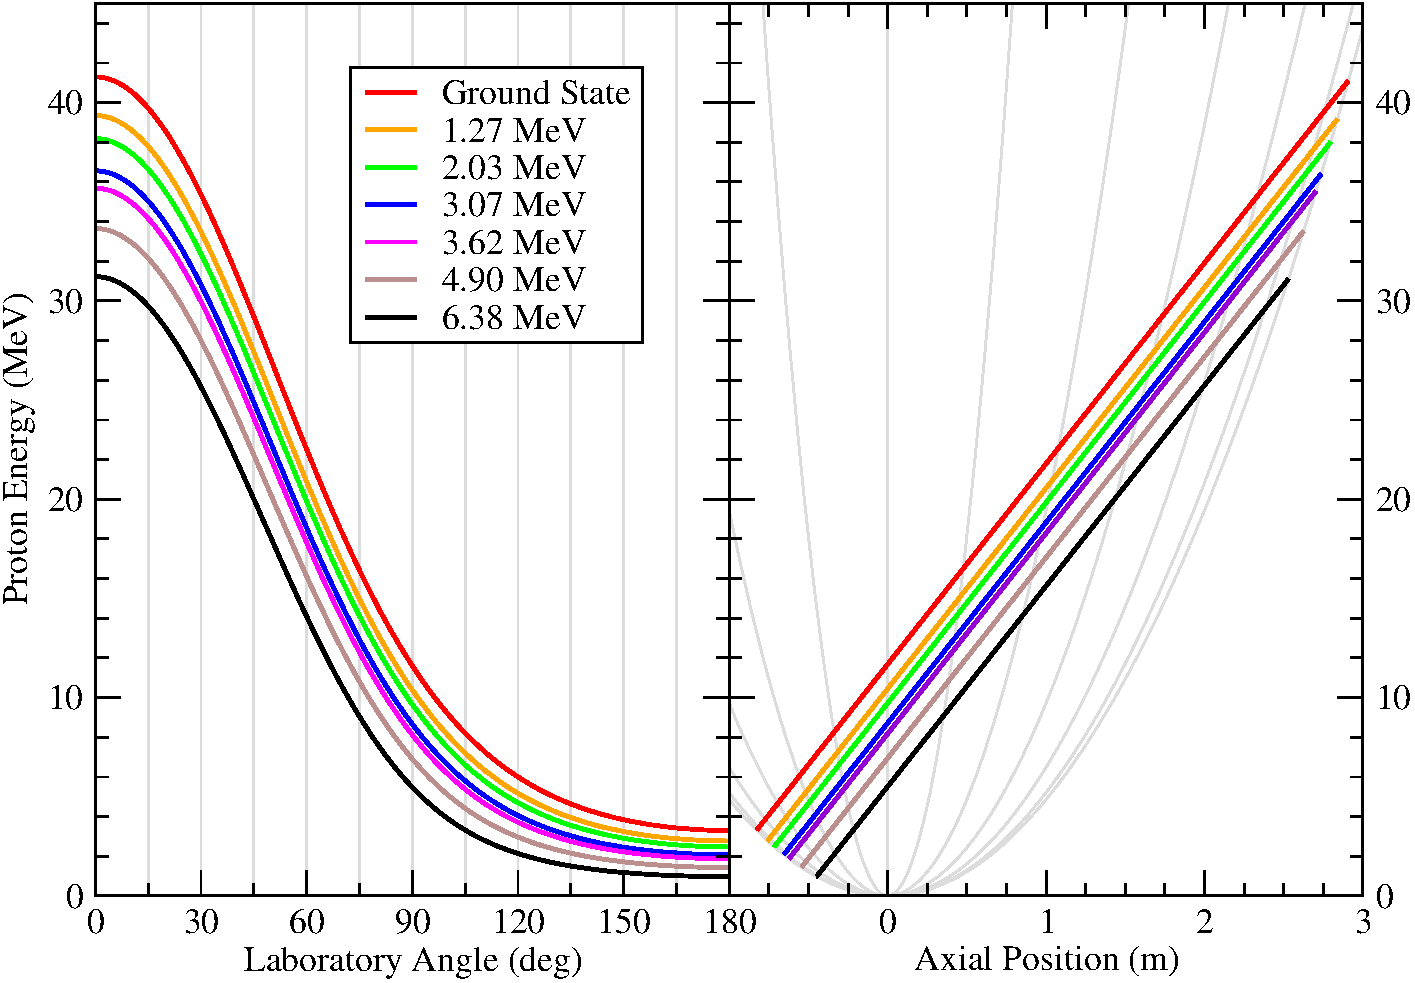
\includegraphics[keepaspectratio,width=\columnwidth,height=0.5\textheight]{si28-plots}%
\caption[Calculated kinematic groups from the $d$($^{28}$Si,$p$) reaction at 6.0\,\AMeV]{Calculated kinematic groups from the $d$($^{28}$Si,$p$) reaction at 6.0\,\AMeV.  The seven strongest transitions populated in the reaction are plotted.  The measured pair $E$ and $\theta_\mathrm{lab}$ (left) exhibit kinematic compression, while the pair $E$ and $z$ measured in a $\mathscr{B}=2.00$\,T field do not.  Lines of constant laboratory angle are plotted in gray every 15$^\circ$.}%
\label{helios_basic}%
\end{figure}
\subsubsection{Position Dispersion}
As mentioned in \S\,\ref{kin_broad}, kinematic broadening arises from the finite resolution of any realistic detector  system when measuring covariant coordinates. % A %canonical 
%$Q$-value measurement requires the measurement of more than one quantity laboratory quantity, typically energy $E_\mathrm{lab}$ and scattering angle $\theta_\mathrm{lab}$.
The degree of covariance between the measured quantities %y measured with the least precision that limits 
determines the contribution of the individual resolutions % of the measured quantities 
to the final $Q$-value resolution.  %In HELIOS, the measured pair is transformed to energy $E_\mathrm{lab}$ and axial position $z_{n}$.
The effect of covariance is intimately related to the effect of kinematic compression, which alters the laboratory spacing of center-of-mass energy levels.  The combined effect of covariance and kinematic compression can be gauged by the \textit{relative} spacing of the individual covariant quantities---that is, the laboratory spacing divided by the resolution.%, $\Delta x/ \delta x$.

An alternate approach to determining the center-of-mass quantities is based on the separation in $z$ of kinematic loci at a fixed energy $E_\mathrm{lab}$.  In a manner similar to the procedure describe above, the kinematic groups can be rotated by a linear transformation and projected onto the position axis to produce a spectrum independent of $E_\mathrm{lab}$.  Rewriting Eq.~\ref{ecm} to solve for $z_1$ yields
\begin{equation}
\begin{split}
z_1=\frac{T_\mathrm{cyc}}{m V_\mathrm{cm}}\left(E_\mathrm{lab}-E_\mathrm{cm}+\frac{1}{2}m V_\mathrm{cm}^2\right).
\end{split}
\label{eq:z_new}
\end{equation}
The position of the $z$-intercept of these lines, corresponding to $E_\mathrm{lab}=0$, is then given by 
\begin{equation}
\begin{split}
z\big|_{E_\mathrm{lab}=0}&=\frac{-mV_\mathrm{cm}}{T_\mathrm{cyc}}\left(E_\mathrm{cm}-\frac{1}{2}m V_\mathrm{cm}^2\right)
\end{split}
\label{x_intercept}
\end{equation}
and the separation between states at a fixed $E_\mathrm{lab}$ is then given by 
\begin{equation}
\begin{split}
\Delta z_1&=\frac{T_\mathrm{cyc}}{m V_\mathrm{cm}}\Delta E_\mathrm{cm}\\
        &=\frac{2 \pi}{\mathscr{B}q V_\mathrm{cm}}\Delta E_\mathrm{cm}.
\end{split}
\label{eq:delta_z}
\end{equation}
Here the ``compression coefficient'' $\Delta z/\Delta E_\mathrm{cm}$ has units of mm/MeV, and is more accurately described as the dispersion in $z$.  So whereas the dispersion in $E_\mathrm{lab}$ is fixed, the dispersion in $z$ is set by the parameters of the experiment, namely the field strength $\mathscr{B}$ and the bombarding energy of the beam.    For example, this coefficient has a value of 98.7\,mm/MeV for the $d$($^{28}$Si,$p$)$^{29}$Si reaction at 6.02\,\AMeV{} and a field strength of 2.00\,T.

In order to assess the possible advantage of using the $z$ dispersion to derive a $Q$-value spectrum, the relative spacing in $z$ must be compared to the relative spacing in $E$.  %All of the quantities in the compression coefficient are known to a higher precision than either the position or energy and thus do not effect the translation.
The uncertainty in $z$, \textit{i.e.} the width of the lines projected onto the $z$ axis, is calculated by adding in quadrature the intrinsic position resolution and the contribution of the energy resolution, based on the slope,  as follows  
\begin{equation}
\begin{split}
\left(\delta z_\mathrm{cm}\right)^2&=\left(\frac{\partial z_\mathrm{cm}}{\partial z}\right)^2\left(\delta z\right)^2+\left(\frac{\partial z_\mathrm{cm}}{\partial E_\mathrm{lab}}\right)^2\left(\delta E_\mathrm{lab}\right)^2\\
%&=\left(\delta z\right)^2+\left(\frac{T_\mathrm{cyc}}{mV_\mathrm{cm}}\right)^2\left(\delta E_\mathrm{lab}\right)^2\\
&=\left(\delta z\right)^2+\left(\frac{2 \pi}{\mathscr{B}q V_\mathrm{cm}}\right)^2\left(\delta E_\mathrm{lab}\right)^2
\end{split}
\label{eq:z_thick}
\end{equation}
where $z_\mathrm{cm}$ is given in analogy to $E_\mathrm{cm}$ in Eq.~\ref{eq:delta_z4}.  The relative resolution, or resolving power, based on the position and the energy are related by
\begin{equation}
\begin{split}
\frac{\Delta z}{\delta z_\mathrm{cm}} =\frac{2 \pi}{\mathscr{B}q V_\mathrm{cm}}\left(\frac{\Delta E_\mathrm{cm}}{\delta E}\right).
\end{split}
\label{eq:delta_z2}
\end{equation}  	%\note{This expression is wrong.  It needs to include the contribution of the energy resolution to the position resolution.  This is an almost identical problem to determining the time resolution required to straighten out the knees.  However, the interest in this situation is to determine the magnetic field strength and bombarding energy to possibly utilize the dispersion characteristics of HELIOS to extract a higher-resolution measurement.}

Table~\ref{dispersion} shows the $z$-dispersion compression coefficients and resolving power for a number of different reaction performed with HELIOS, using intrinsic resolution values $\delta z=1.0$\,mm~FWHM  and $\delta E_\mathrm{lab}=40$\,keV~FWHM.   The relative resolution is calculated for states assuming $\Delta E_\mathrm{cm}=1$\,MeV.  As Table~\ref{dispersion} shows, any possible advantage gained by the $z$-dispersion tends to be canceled out by the line width $\delta z_\mathrm{cm}$ and there is no improvement in the resolving power.  Utilizing the variable dispersion may allow one to compensate for kinematic broadening under certain circumstances.  However, this technique has limited applicability because the field strengths at which the technique is beneficial ($\mathscr{B}<1$\,T), reduces the acceptance of the spectrometer. 

\begin{table*}%
  \centering
  \begin{tabular}{,d{2}cd{1}ccc}
    \hline
    \multicolumn{1}{c}{\multirow{2}{*}{Reaction}}  &
    \multicolumn{1}{c}{$E_1/A_1$}  &
    \multicolumn{1}{c}{$\mathscr{B}$}  &
    \multicolumn{1}{c}{$\Delta z/\Delta E_\mathrm{cm}$}&
    $\delta z_\mathrm{cm} $ & $\Delta z/ \delta z_\mathrm{cm}$ & $\Delta E_\mathrm{cm}/\delta E$\\
    
      &\multicolumn{1}{c}{(\AMeV)}&
    \multicolumn{1}{c}{(T)}&
    \multicolumn{1}{c}{(mm/MeV)} & 
    \multicolumn{1}{c}{(mm)}  &  
   \multicolumn{1}{c}{---}&
   \multicolumn{1}{c}{---}\\
    \hline \hline
    d(^{28}\textrm{Si},p)^{29}\textrm{Si} 	& 6.02 & 2.00 & 98.7 & 4.1 & 24.2 & 24.2\\
    d(^{12}\textrm{B},p)^{13}\textrm{B} 	 &6.24 & 1.04 & 202.8 & 8.2 & 24.8 & 24.8\\
    d(^{132}\textrm{Sn},p)^{133}\textrm{Sn}	 &4.78 & 2.00 & 105.1 & 4.3 & 24.3 & 24.3\\
    d(^{124}\textrm{Sn},^3\textrm{He})^{123}\textrm{In} 	 &13.00 & 2.73 & 23.3 & 1.4 & 17.1 & 16.6\\
    p(^{77}\textrm{Kr},d)^{76}\textrm{Kr}  	 &30.00 & 2.00 & 41.8 & 1.9 & 21.5 & 21.3\\
    \hline
  \end{tabular}
  \caption[Compression coefficients based on the dispersion in $z$ using HELIOS]{Compression coefficients based on dispersion the in $z$ using HELIOS.  The compression in $z$ is given as the inverse-slopes of the kinematic loci, $\Delta z/\Delta E_\mathrm{cm}$. The two rightmost columns give the relative resolving power, where a higher number corresponds to higher resolving power.}
  \label{dispersion}
\end{table*}

\subsection{The Acceptance}
\label{accept}
In a traditional detector scheme, the acceptance or solid angle coverage is defined by the range of angles subtended by the detector ($\theta$,$\phi$)---in other words, the fraction of a sphere surrounding the target covered by detectors.  In the HELIOS detector scheme, the solenoid transports the ions in such a way as to ostensibly redefine the acceptance as the fraction of area coved on a cylinder on the solenoid axis ($z$,$\phi$).
\subsubsection{Calculating the Solid Angle}
The solid angle coverage for an individual detector element in HELIOS is given by
\begin{equation}
\begin{split}
\Omega&\equiv\iint_{S}\sin(\theta)\mathrm{d}\theta\mathrm{d}\phi\\
%&=\phi]_{\phi_1}^{\phi_2} \cos(\theta)]\\
&=\Delta \phi[\Delta \cos(\theta)]\\
&=[2\arctan(w_0/2\rho_0)][\Delta \cos(\theta)]\\
\end{split}
\label{solid_ang}
\end{equation}
where $w_0$ is the width of the detector and $\rho_0$ is the radius of the detector array.

Given the relation $z_1=v_\parallel T_\mathrm{cyc}=[v_{0}\cos(\theta_\mathrm{cm})+V_\mathrm{cm}]T_\mathrm{cyc}$, each detector subtends the same range of $\cos(\theta_\mathrm{cm})$.  Here $\cos(\theta)$ is given by
\begin{equation}
\cos(\theta_\mathrm{cm})=\dfrac{z/t-V_\mathrm{cm}}{v_0}
%\cos(\theta_\mathrm{cm})=\dfrac{\dfrac{z}{\left(T_\mathrm{cyc}-\dfrac{\rho_0}{v_0 \sin(\theta_\mathrm{cm})}\right)}-V_\mathrm{cm}}{v_0}
\label{new_costhetacm}
\end{equation}
where $t$ is the time of flight, given in Eq.\,\ref{time_of_flight}.  The actual range of angles covered in the center-of-mass
frame depends on the position of
the array.  As shown in Eq.~\ref{eq:delta_z}, the dispersion and thus the solid-angle acceptance also depends on the magnetic field and the bombarding energy studied.  An increase in the magnetic field decreases the dispersion 
and thus increases the coverage in center-of-mass angles for a given detector
position.  Similarly for the bombarding energy.

\subsubsection{Example}
For the
ground-\-state transition in the $d$($^{28}\mathrm{Si},p$)$^{29}$Si reaction at
6\,\AMeV{} with a central magnetic field of 2.0\,T, each detector subtends between 2--5$^\circ$ in the center-of-mass frame, depending on its distance from the target.  As seen from Fig.~\ref{analytic}, the range of
center-of-mass angles covered for the entire array is 21--42$^\circ$ given the interval covered by the array is between $-680$ and $-340$\,mm from the target.   With these settings, each detector
covers an interval of $\Delta \cos(\theta_\mathrm{cm})=0.028$ and 
covers an azimuthal range of $\Delta \phi = 0.24\pi$, giving a solid angle of 0.021\,sr per
element, and a total solid angle coverage of 0.50\,sr for the silicon
array in the center-of-mass frame.

%\subsection{Geometric Constraints}
\subsubsection{Radial Acceptance}
For particle orbits originating on the solenoid axis, as is the case in HELIOS, the radial excursion goes as $\rho=r[1-\cos(\varphi)]$ with a maximum of $\rho=2r$.  This radial extreme is related to the laboratory energy by
\begin{equation}
\begin{split}
%v_\mathrm{lab}\sin(\theta_\mathrm{lab})&=\frac{rq\mathscr{B}}{m}\\
v_\mathrm{lab}\sin(\theta_\mathrm{lab})&=\frac{2\pi r}{T_\mathrm{cyc}}\\
v_\mathrm{lab}&=\frac{rq\mathscr{B}}{m\sin(\theta_\mathrm{lab})}\\
E_\mathrm{lab}&=\frac{1}{2m}\left(\frac{(\rho/2)q\mathscr{B}}{\sin(\theta_\mathrm{lab})}\right)^2\\
\end{split}
\label{rho_limit}
\end{equation}
When $\rho$ is the radius of the solenoid bore, Eq.~\ref{rho_limit} gives the high-energy acceptance cutoff imposed by the size of the solenoid.  This limit is plotted with a wide-dashed line in various single-orbit energy versus position spectra (\textit{e.g.}, Figs.~\ref{analytic} and \ref{b11_spec}).  When $\rho=\rho_0$, the radius of the detector array, the limit imposed by the radial extent of the array is given.  However, this theoretical limit is not typically the effective limit.  The minimum-radius orbit acceptance of the array is not typically determined by the radial excursion of the orbit, but by the emission angle.  For a given target-to-detector separation $\Delta z$, the minimum angle is given by $\theta_\mathrm{lab}=\arctan(\rho_0/\Delta z)$.  This limit is plotted in various $E_\mathrm{lab}$ vs. $z$ histograms, represented by a narrow-dashed line.

Eq.~\ref{rho_limit} may be rewritten in terms of the momentum $p$ of the ejectile using the relation $E=p^2/(2m)$.  Using this formulation, the axial acceptance can be written in terms of magnetic rigidity\footnote{The magnetic rigidity is typically written as $\mathscr{B}\rho$ (``bee-rho'') where $\rho$ is the radius of curvature of the particle orbit, defined here as $r$.} $\mathscr{B}r$. 

\begin{equation}
\begin{split}
p_\mathrm{lab}&=\frac{(\rho/2)q\mathscr{B}}{\sin(\theta_\mathrm{lab})}\\
p_\mathrm{lab}&=\frac{rq\mathscr{B}}{\sin(\theta_\mathrm{lab})}\\
p_\perp&=rq\mathscr{B}\\
\mathscr{B}r&=\frac{p_\perp}{q}\\
\end{split}
\label{B-rho}
\end{equation}

\subsubsection{Axial Acceptance}
Ref.~\cite{Wuosmaa_2007} includes an expression similar to Eq.~\ref{rho_limit} for determining the $z$-acceptance of the array.\footnote{The equation given in Ref.~\cite[Eq.~11]{Wuosmaa_2007} contains a typographical error.  The ``$\cos$'' terms are meant to be ``$\sin$.''}  Whereas Eq.~\ref{rho_limit} is based on $v_\perp$, the $z$-acceptance is based on $v_\parallel$ as follows
\begin{equation}
\begin{split}
v_\mathrm{lab}\cos(\theta_\mathrm{lab})%&=z/t\\
&=z_1/T_\mathrm{cyc}\\
%&=\frac{z_1q\mathscr{B}}{2\pi m}\\
v_\mathrm{lab}&=\frac{z_1q\mathscr{B}}{2\pi m \cos(\theta_\mathrm{lab})}\\
E_\mathrm{lab}&=\frac{1}{2m}\left(\frac{z_1q\mathscr{B}}{2\pi \cos(\theta_\mathrm{lab})}\right)^2\\
\end{split}
\end{equation}
\par The maximum axial excursion---which is included here as part of the discussion of the ac\-cep\-tance---re\-quires the consideration of the effect of a finite detector array, which is discussed in the following section.   The maximum axial excursion is found by taking the partial derivative of Eq.~\ref{z_offset} (on page~\pageref{z_offset}).  The extremum occurs when the condition given in Eq.~\ref{knee_eq} is satisfied, which assumes $\rho_0/2r\ll 1$.  This point occurs at approximately a fixed value of $\theta_\mathrm{cm}$ for the energy levels populated in a given reaction.  For example, in the $d$($^{28}$Si,$p$)$^{29}$Si reaction %discussed in \S\,\ref{detail}
illustrated in Fig~\ref{analytic}, the maximum longitudinal excursion occurs at approximately 8$^\circ$ %proton forward
in the center-of-mass frame.  
\begin{equation}
\begin{split}
\frac{\partial}{\partial \theta_\mathrm{cm}}z&=-v_0\sin(\theta_\mathrm{cm})T_\mathrm{cyc}
%\\&\qquad
+\frac{\rho_0}{v_0\sin^2(\theta_\mathrm{cm})}[V_\mathrm{cm}\cos(\theta_\mathrm{cm})+v_0]\\
\frac{\partial}{\partial \theta_\mathrm{cm}}z&=0\qquad \textrm{critical point condition}\\
v_0\sin(\theta_\mathrm{cm})T_\mathrm{cyc}&=\frac{\rho_0}{v_0\sin^2(\theta_\mathrm{cm})}[V_\mathrm{cm}\cos(\theta_\mathrm{cm})+v_0]
%0&=-v_0\sin(\theta_\mathrm{cm})T_\mathrm{cyc}+\frac{\rho_0}{v_0\sin^2(\theta_\mathrm{cm})}[V_\mathrm{cm}\cos(\theta_\mathrm{cm})+v_0]
\end{split}
\label{knee_eq}
\end{equation}
Note that when $\rho_0=0$, $z$ reaches a maximum at the expected value of $z_1=-v_0\sin(\theta_\mathrm{cm})T_\mathrm{cyc}$.

\section{Considerations}
\subsection{The Effect of a Finite Detector}
\label{finite}
So far in this chapter, the equations are valid for any charged particle moving in a homogeneous magnetic field---trajectories begin and end on the magnetic field axis and the time of flight of the orbits is equal to $T_\mathrm{cyc}$.
%\note{The relationship given in [2, Eq. 5] is an idealization which assumes a detector array of zero radius, with the detected position $z$ equal to the axis intercept $z_1$.}  
However, in order to be detected, particles must be intercepted by the detector array before returning to the solenoid axis, thereby truncating the trajectory of the particle.  This process is illustrated in Fig.~\ref{orbit_fig}.
\begin{figure}%
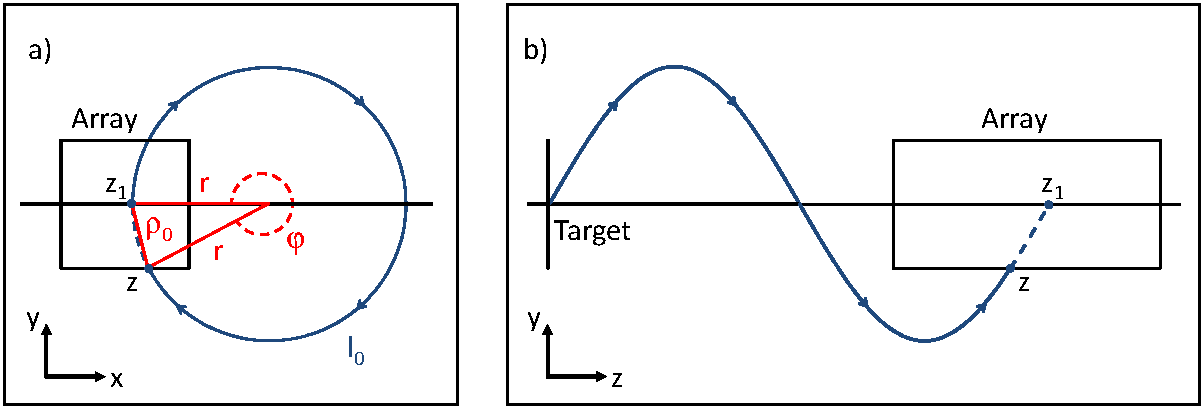
\includegraphics[width=\columnwidth]{array}
\caption[Illustration of a typical particle orbit intersecting a finite array]{Illustration of a typical particle orbit intersecting a finite array. a) The end-view of the array shows the transverse orbit length $l_0$ is truncated by the radius of the array $\rho_0$. b) The side-view of the array shows the relationship between $z$ the detection distance and $z_1$ the axis intercept.}%
\label{orbit_fig}%
\end{figure}
  The axis intercept $z_1$ is slightly greater in magnitude than the position where the particle is detected $z$ due to the finite transverse extent of any given detector array.  Similarly, the time of of flight $t$ is reduced from $T_\mathrm{cyc}$.  
\subsubsection{Formulation}
The effect of a finite detector array may be formulated in terms of its effect on the path length of a particle orbit.  The transverse path length of a particle orbit may be written as $l_0=\varphi r$ where $\varphi$ is the angle of rotation about the orbit's center.  For a detector of ``radius'' $\rho_0$, the path length of a single orbit $l_0$ is given by 
\begin{equation}
\begin{split}
{l_0}&=r(2\pi-\varphi_0)\\
&=r\left[2\pi-2\arcsin\left(\dfrac{\rho_0}{2r}\right)\right]\\
&\approx 2\pi r-\rho_0
\end{split}	
\label{trans_path}
\end{equation}
where $\varphi_0$ is the angle of the cyclotron orbit excluded by the detector array.  For a detector array with a non-circular (polygonal) cross section, the radius $\rho_0$ is a function of the azimuthal coordinate $\phi$.  In such case, a fixed $z$-position corresponds to a finite range of radii.  This leads to a variation in energy for a given transition at a fixed $z$, which is an example of kinematic broadening.
%For a detector array with a polygonal cross section $\rho_0$ is a function of $\phi$, the azimuthal coordinate.
  Thus, the detected position is given by 
\begin{equation}
\begin{split}
z&=v_\parallel t\\
&=v_\parallel \left(\frac{l_0}{v_{\perp}}\right)\\
%&=v_\| \left(\frac{r(2\pi-\phi)}{v_{\perp}}\right)\\
%z_\parallel
&=(v_{0}\cos(\theta_\mathrm{cm})+V_\mathrm{cm})\frac{r\left[2\pi-2\arcsin\left(\dfrac{\rho_0}{2r}\right)\right]}{v_0\sin(\theta_\mathrm{cm})}.
\end{split}	
\label{z_defined}
\end{equation}
\par As shown in Eq.~\ref{trans_path}, the transverse path length of the cyclotron orbit is reduced from 2$\pi r$ by approximately $\rho_0$, the radius of the detector array.  This approximation is valid when the quantity $\rho_0/2r$ is sufficiently small ($\ll1$).  Due to the acceptance limit imposed by a realistic detector array (see \S\,\ref{accept}), this condition is always true for detected particles.  Given this approximation, the relationship between the detected position of the ions $z$ and  the axis intercept $z_1$ is given by
\begin{equation}
\begin{split}
%&\approx(v_{0}\cos(\theta_\mathrm{cm})+V_\mathrm{cm})\frac{r\left[2\pi-2\left(\dfrac{\rho_0}{2r}\right)\right]}{v_0\sin(\theta_\mathrm{cm})}\\
z&\approx(v_{0}\cos(\theta_\mathrm{cm})+V_\mathrm{cm})\left(\frac{2\pi r-\rho_0}{v_0\sin(\theta_\mathrm{cm})}\right)\\
	 &=(v_{0}\cos(\theta_\mathrm{cm})+V_\mathrm{cm})\left(T_\mathrm{cyc}-\frac{\rho_0}{v_{0}\sin(\theta_\mathrm{cm})}\right)\\
&=v_\mathrm{lab}\cos(\theta_\mathrm{lab})\left(T_\mathrm{cyc}-\frac{\rho_0}{v_\mathrm{lab}\sin(\theta_\mathrm{lab})}\right)\\
%z_\parallel	 
&= z_1-\frac{\rho_0}{\tan(\theta_\mathrm{lab})}.
\end{split}	
\label{z_offset}
\end{equation}
Therefore, the deviation from the zero-radius detector limit is exaggerated for shallow emission angles with respect to the magnetic field axis, corresponding to smaller helical orbit radii.  The time of flight $t$ is reduced from the cyclotron period $T_\mathrm{cyc}$ in a similar fashion
\begin{equation}
\begin{split}
t&=T_\mathrm{cyc}-\frac{2r}{v_\perp}\arcsin\left(\frac{\rho_0/2}{r}\right) \\
&\approx T_\mathrm{cyc}-\dfrac{\rho_0}{v_0 \sin(\theta_\mathrm{cm})}
\end{split}
\label{time_of_flight}
\end{equation}

In the rearward hemisphere ($\theta_\mathrm{lab}>90^\circ$), the effect of a finite detector array manifests itself in the appearance of ``knees'' %or a ``fish-hook'' shape
 in the kinematic loci.  Fig.~\ref{analytic}(a) shows an analytic calculation of proton energies and center-of-mass angles vs. position for the $d$($^{28}$Si,$p$)$^{29}$Si reaction. The calculation assumes a cylindrical detector array of radius $\rho_0=$11.4\,mm and an ideal solenoid with a uniform field of 2.00\,T.  The effect of a non-zero radius detector array is illustrated by comparing the dotted lines in Fig.~\ref{analytic} with the solid lines corresponding to the ground-\-state transition.
 
In the forward hemisphere ($\theta_\mathrm{lab}<90^\circ$), the effect of a finite detector array is the same, insofar as the detected position $z$ is reduced in magnitude from the axis intercept $z_n$ as given in Eq.~\ref{z_offset}.  However, the velocity $v_\parallel$ and the slope $\partial E_\mathrm{lab}/\partial z$ have opposite sign, leading to a single-valued function of $E_\mathrm{lab}$ vs. $z$ at low energy.  In analogy to the knees mentioned above, this feature may be referred to as a ``heel'' shape.  Fig.~\ref{analytic}(c) shows an analytic calculation of helion energies and center-of-mass angles vs. position for the $d$($^{124}$Sn,$^3$He)$^{123}$In reaction. The calculation assumes a uniform field of 2.73\,T.

\begin{figure*}
\centering
%\includegraphics[width=\linewidth,keepaspectratio,height=0.5\textheight]{../NIM_Paper/Figures/Old_Figures/excel_plots_ab}
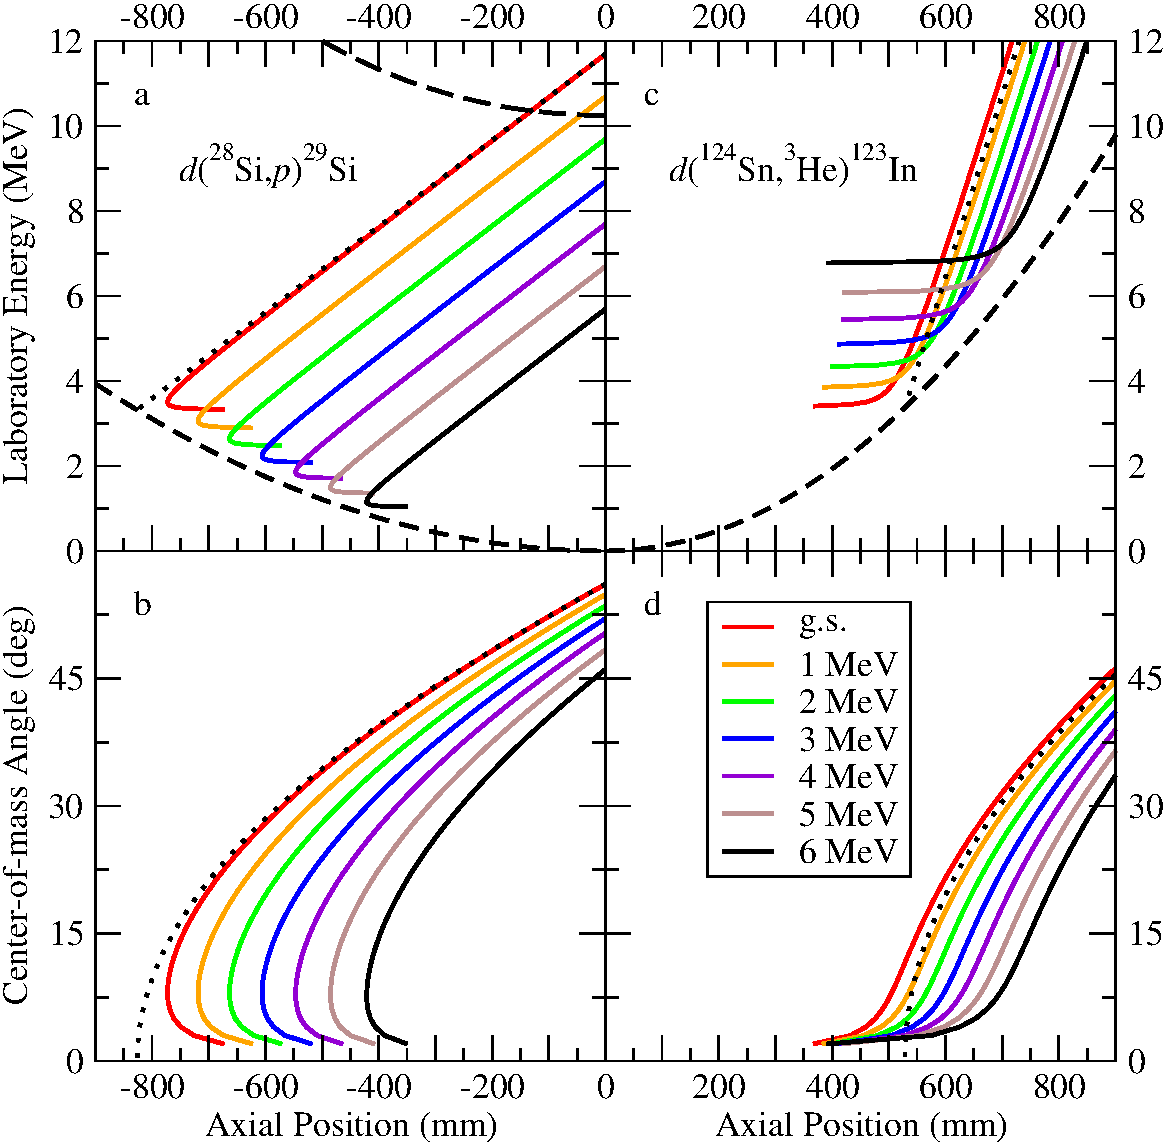
\includegraphics[angle=0,width=\textwidth,height=0.75\textheight,keepaspectratio]{4-kin_tall}
\caption[Calculated ejectile energies for the $d$($^{28}$Si,$p$)$^{29}$Si and $d$($^{124}$Sn,$^3$He)$^{123}$In reactions]{Calculated ejectile energies for the $d$($^{28}$Si,$p$)$^{29}$Si and $d$($^{124}$Sn,$^3$He)$^{123}$In reactions. Panels (a) and (b) correspond to $d$($^{28}$Si,$p$)$^{29}$Si,
 and panels (c) and (d) correspond to $d$($^{124}$Sn,$^3$He)$^{123}$In.
Panels (a) and (c) show the ejectile energy $E_\mathrm{lab}$ vs. detected axial position $z$ (relative to the target) for protons ejected in the rearward hemisphere and helions ejected in the forward hemisphere, respectively.  In panels (b) and (d), the emission angle of the ejectile in the center-of-mass $\theta_\textrm{cm}$ is plotted against the detected position $z$.  Excitation energies were selected such that $\Delta E_\mathrm{cm}=1$\,MeV.  The dotted line in each plot corresponds to the ground-\-state transition as measured by a detector array of zero radius, illustrating the difference between the axis intercept $z_1$ and the detected position $z$.  The dashed line running through panels (a) and (c) represents $\theta_\textrm{lab}=0^\circ$.  The upper dashed line in panel (a) corresponds to the limit imposed by the solenoid bore.  This limit occurs above the axis range in (c).  Both reaction calculations assume an ideal magnetic field of 2.00\,T.}
\label{analytic}
\end{figure*}

%In the forward hemisphere, the shape is 
\subsubsection{Compensation}
As discussed, the relationship given in Eq.~\ref{ecm} is an idealization which assumes a detector array of zero radius, meaning the detected position $z$ is equal to the axis intercept $z_1$.  The deviation from the zero-radius limit is effectively negligible for sufficiently large ejection angles.  The value of this ``threshold'' varies depending on the reaction, but can be seen to be about $\theta_\mathrm{lab}>10^\circ$ in Fig.~\ref{analytic}.  However, below this threshold, in the region of the knees, the offset is significant. In order to correct for this disparity, the time of flight must also be taken into account.  Using the relation $v_\parallel=z_1/T_\mathrm{cyc}=z/t$, Eq.~\ref{ecm} may be rewritten as 
\begin{equation}
E_\mathrm{cm}=E_\mathrm{lab}+\frac{1}{2} mV_\mathrm{cm}^2-\frac{m V_\mathrm{cm}}{t}z.
\label{ecm_new}
\end{equation}
Whereas Eq.~\ref{eq:no_comp} gives the $Q$-value resolution based only on the energy resolution, this reformulation of $E_\mathrm{cm}$ combines all three measured quantities.   

\begin{equation}
\begin{split}
\left(\delta E_\mathrm{cm}\right)^2&=\left(\frac{\partial E_\mathrm{cm}}{\partial E_\mathrm{lab}}\right)^2\left(\delta E_\mathrm{lab}\right)^2+\left(\frac{\partial E_\mathrm{cm}}{\partial z}\right)^2\left(\delta z\right)^2+\left(\frac{\partial E_\mathrm{cm}}{\partial t}\right)^2\left(\delta t\right)^2+2\left(\frac{\partial E_\mathrm{cm}}{\partial z}\right) \delta z \left(\frac{\partial E_\mathrm{cm}}{\partial t}\right)\delta t\\
\left(\delta E_\mathrm{cm}\right)^2&=\left(\delta E_\mathrm{lab}\right)^2+\left(\frac{-m V_\mathrm{cm}}{t}\right)^2\left(\delta z\right)^2+\left(\frac{m V_\mathrm{cm}}{t^2}z\right)^2\left(\delta t\right)^2+2\left(\frac{-m V_\mathrm{cm}}{t}\right) \delta z \left(\frac{m V_\mathrm{cm}}{t^2}z\right)\delta t
\end{split}
\label{eq:delta_z3}
\end{equation}

The excitation energy can be determined in the region of the knees with a sufficiently fine time resolution. Table~\ref{time_res} shows the contribution of the time resolution to the overall $Q$-value resolution.  However, with the prototype array discussed in \S\,\ref{charact} having a time resolution of $\delta t=3.87$\,ns, this correction has a prohibitively deleterious effect on the final $Q$-value resolution. 

\begin{table*}%
  \centering
  \begin{tabular}{lcc|cccrr}		
    \hline
    \multicolumn{1}{c}{\multirow{2}{*}{Reaction}}  &
    \multicolumn{1}{c}{$E_1/A_1$}  &
    \multicolumn{1}{c}{$\mathscr{B}$}  &
    \multicolumn{1}{c}{$\delta t$} & 
    \multicolumn{3}{c}{Origin of contribution}  &
    \multicolumn{1}{c}{$\delta E_\textrm{cm}$}  \\  \cline{5-7}
    &\multicolumn{1}{c}{(\AMeV)}&
    \multicolumn{1}{c}{(T)}&
    \multicolumn{1}{c}{(ns)}&
    \multicolumn{1}{c}{$\delta z$}  &  
    \multicolumn{1}{c}{$\delta E_\textrm{lab}$} & 
    \multicolumn{1}{c}{$\delta t$} & 
    \multicolumn{1}{c}{(keV)}\\
    \hline \hline 
    %\multirow{5}{*}{$d$($^{28}\textrm{Si}$,$p$)$^{29}\textrm{Si}$} 	 &3.87 & 50 & 5 & 480 & 485\\
    $d$($^{28}\textrm{Si}$,$p$)$^{29}\textrm{Si}$ &6.02&2.00
      &5.00 & 11 & 40 & 1,280 & 1,280\\
    &&&2.00 & 11 & 40 & 511 & 512\\
    &&&1.00 & 11 & 40 & 256 & 256\\
    &&&0.50 & 11 & 40 & 128 & 131\\
    &&&0.25 & 11 & 40 & 64 & 70\\
    \hline
  \end{tabular}
  \caption[Calculated contribution of $\delta t$ to the uncertainty in $E_\mathrm{cm}$]{Calculated contribution of $\delta t$ to the uncertainty in $E_\mathrm{cm}$.  Contributions are given in keV~FWHM and are tabulated 
    for several values of $\delta t$, holding $\delta E_\mathrm{lab}$ and 
    $\delta \theta_\mathrm{lab}$ fixed.  The values are calculated at $\theta_\mathrm{cm}=10^\circ$.}
  \label{time_res}
  \end{table*}

\subsection{Corrections for Relativity}
So far in this chapter, the effects of relativity have been ignored.  However, with heavy-ion reactions such as $^{132}$Sn($d$,$p$) planned to be measured with HELIOS at beam energies in the GeV-range, it is important to ensure that this premise is valid.  Stating the problem in terms of velocities and inertial frames, $v_\mathrm{lab}$ is the velocity of the projectile in the (stationary) laboratory frame; the center-of mass frame is moving with a velocity of $V_\mathrm{cm}$ relative to the laboratory frame in the $+z$ direction; and $v_0$ is the velocity of the ejectile in the center-of-mass frame.
\subsubsection{Transformation Factors}
Here, we have a choice of how best to keep the notation both brief and consistent.  The velocities $v_\mathrm{lab}$,$v_0$, and $V_\mathrm{cm}$ have been clearly defined; % and used consistently.  T
 therefore, the speed parameters may be written as $\beta$,$\beta_0$,$B_\mathrm{cm}$ and the Lorentz factors as $\gamma$,$\gamma_0$,$\Gamma_\mathrm{cm}$. 	
The velocity of the center-of-mass is defined in terms of the speed parameter $B_\mathrm{cm}=V_\mathrm{cm}/c$ where $c$ is the speed of light and $B_\mathrm{cm}$ is given by 
\begin{equation}
\begin{split}
B_\mathrm{cm}%&=\frac{P_1}{W_t}\\
%&=\frac{p_1c}{W_t}\\
&=\frac{p_1c}{\gamma_1 m_1c^2+m_2c^2}\\
&=\frac{\sqrt{E_1^2+2m_1c^2E_1}}{E_1+(m_1+m_2)c^2}.
\end{split}
\label{big_beta}
\end{equation}
Here the subscripts on $m_1$ and $m_2$ refer to the masses of the incident beam particle and the target particle, respectively.  The momentum $p_1$ and total energy $\gamma_1 m_1c^2$ of the beam particle are rewritten in terms of the total beam energy $E_1$ (\textit{cf}.~\citet[Eq.~7.98]{Goldstein_2002}).  The Lorentz factor for the center-of-mass frame is then written as $\Gamma_\mathrm{cm}=1/\sqrt{1-B_\mathrm{cm}^2}$.

\subsubsection{Energy}
With the total energy in the laboratory frame given by $W_t=E_1+(m_1+m_2)c^2$, the total energy in the center-of-mass frame is $W_t^\prime=W_t/\Gamma_\mathrm{cm}$.  Here, prime notation refers to quantities in the center-of-mass system.  With $W_t^\prime$ defined, the total energy of the ejectile in the center-of-mass is given by 
\begin{equation}
\begin{split}
W^\prime&=\frac{(W_t^\prime)^2+(m-M)c^2}{2W_t^\prime}
\end{split}
\label{eq:E_rel}
\end{equation}
where $m$ and $M$ are the mass of the ejectile and heavy recoil, respectively.  The excitation energy enters Eq.~\ref{eq:E_rel} implicitly via the heavy ion mass, given $M=M_0+E_x$.  Similarly, the reaction $Q$-value is represented in the particle masses (\textit{cf}. Eq.~\ref{eq:q_value}). Finally, the kinetic energy of the ejectile is given as a function of scattering angle as 
\begin{equation}
\begin{split}
E&=W-mc^2\\
&=W^\prime \Gamma_\mathrm{cm}(1+ B_\mathrm{cm} \beta_0 \cos(\theta_\mathrm{cm}))-mc^2
\end{split}
\label{eq:E_rel2}
\end{equation}

\subsubsection{Velocities}
The trajectories within HELIOS are defined by the velocity projections.  Using the standard ve\-loc\-i\-ty-ad\-di\-tion formula based on the Lorentz transformation, the axial velocity may be written as
\begin{equation}
\begin{split}
v_\parallel&=\frac{v_\parallel^\prime+V_\mathrm{cm}}{1+v_\parallel^\prime V_\mathrm{cm}/c^2}\\
&=\frac{v_0\cos(\theta_\mathrm{cm}) + V_\mathrm{cm}}{1+[v_0\cos(\theta_\mathrm{cm})]V_\mathrm{cm}/c^2}\\
&=\frac{v_0\cos(\theta_\mathrm{cm}) + V_\mathrm{cm}}{1+B_\mathrm{cm}\beta_{0}\cos(\theta_\mathrm{cm})}
%&=\frac{v_\parallel^\prime}{1+B_\mathrm{cm}\beta_{0}\cos(\theta_\mathrm{cm})}
\end{split}
\label{eq:rel_v_x}
\end{equation}
where $v_\parallel^\prime$ is the $z$-projection of the ejectile velocity in the center-of-mass frame.  Similarly, the radial velocity may be written as
\begin{equation}
\begin{split}
v_\perp&=\frac{v_\perp^\prime}{\Gamma_\mathrm{cm}(1+v_\parallel^\prime V_\mathrm{cm}/c^2)}\\
&=\frac{v_0 \sin(\theta_\mathrm{cm})}{\Gamma_\mathrm{cm}[1+B_\mathrm{cm}\beta_{0}\cos(\theta_\mathrm{cm})]}
\end{split}
\label{eq:rel_v_y}
\end{equation}
With these velocity transformations, the scattering angle in the laboratory $\theta_\mathrm{lab}$ is derived in the usual way
\begin{equation}
\begin{split}
\tan(\theta_\mathrm{lab})&=v_\perp/v_\parallel\\
&=\frac{v_0\sin(\theta_\mathrm{cm})}{\Gamma_\mathrm{cm}[v_0\cos(\theta_\mathrm{cm}) + V_\mathrm{cm}]}\\
&=\frac{1}{\Gamma_\mathrm{cm}}\frac{\sin(\theta_\mathrm{cm})}{\cos(\theta_\mathrm{cm})+K}
\end{split}
\label{eq:new_angle}
\end{equation}
Here $K$ retains its definition as $V_\mathrm{cm}/v_0$, but may be rewritten as $B_\mathrm{cm}/\beta_0$ (\textit{cf}.~\citet[Eq.~7.112]{Goldstein_2002}, \citet[Eq.~3.2]{Michalowicz_1967}).
\subsubsection{Cyclotron Orbit}
The cyclotron motion is defined by the velocity perpendicular to the magnetic field $v_\perp$.  As such, the relevant Lorentz factor is defined as $\gamma_\perp=1/\sqrt{1-(v_\perp/c)^2}$.  The equations of the cyclotron orbit may then be rewritten.
Eq.~\ref{cyc_rad} becomes
\begin{equation}
\begin{split}
r=v_{\perp}\frac{\gamma_\perp m}{\mathscr{B}q}\\
\end{split}
\label{rel_cyc_rad}
\end{equation}
and Eq.~\ref{Tcyc} becomes
\begin{equation}
T_\mathrm{cyc}=\frac{2\pi}{\mathscr{B}} \left(\frac{\gamma_\perp m}{q}\right)
\label{rel_Tcyc}
\end{equation}
%With these corrections the remainder of the equations relevant to calculating kinematics within HELIOS remain unchanged from \S\,\ref{}
\subsubsection{Example}
To use a representative example, consider the $^{124}$Sn($d$,$^3$He) reaction at 13\,\AMeV.  At the time of this writing, this reaction has the highest kinetic energy of any approved HELIOS experiment.  At the quoted energy, the $^{124}$Sn beam ion has a kinetic energy of $T=1.61$\,GeV and a rest mass of $m_0 c^2=115$\,GeV.  Even at this comparatively high energy, the collision is still in the classical energy regime of $T\ll m_0 c^2$, with $\gamma_0=1.01$.

With $K=1.42$, the energy solution is double-valued in the laboratory with a maximum ejection angle of $\theta_\mathrm{lab}=44.6^\circ$.  Taking relativistic kinematics into consideration, the maximum correction to the classically-calculated energy for a given $\theta_\mathrm{cm}$ scattering angle is 0.49\%.  For the high-energy solution, neglecting this correction corresponds to a calculation error of less than 500\,keV.  However, in the range of energies relevant to the prototype silicon detector array, which has a sensitivity of about 1--12\,MeV, this correction has an RMS value of 13\,keV\label{typo5}.  Therefore, for the purposes of calculating---and simulating---particle trajectories within HELIOS in order to determine an optimal experimental setup, the effects of relativity are negligible. 

\subsection{Technical Requirements}
It is useful here to briefly review the technical requirements to realize the HELIOS concept; these requirements are discussed in Ref.~\cite{Wuosmaa_2007} and summarized in Table~\ref{helios_req}.  The solenoid should have a radial parameter $\mathscr{B}r$ on the order of 1.25\,T$\cdot$m and a length parameter $\mathscr{B}L$ on the order of 3.5\,T$\cdot$m.  Standard ``3\,T'' Magnetic Resonance Imaging (MRI) medical scanners match these requirements.  For particle identification, a detector timing resolution of approximately 10\,ns is needed to separate particle groups with different values of $A/q$.  In order to straighten the knees of kinematic groups, timing resolution below 0.50\,ns is required; however, this feature is not necessarily required for successful operation of the spectrometer.  In order to take advantage of the $Q$-value resolution provided by the HELIOS measurement approach, certain limits need to be placed on the position and energy resolution of the detector array.  Position resolution on the order of 0.5--1.0\,mm~FWHM is required.  Energy resolution on the order of 25--50\,keV~FWHM is required.  The following chapters discuss how the actual performance characteristics of the HELIOS spectrometer compare to these requirements.

\begin{table}[b]
\centering
\begin{tabular}{ccccccccc}
\hline
\multicolumn{2}{c}{Solenoid}  &  &
\multicolumn{3}{c}{Detectors}  & & 
\multicolumn{2}{c}{Derived}\\ \cline{1-2} \cline{4-6} \cline{8-9}
\multicolumn{1}{c}{$\mathscr{B}R$}  &  
\multicolumn{1}{c}{$\mathscr{B}L$}  & &
\multicolumn{1}{c}{$\delta z$}  &  
\multicolumn{1}{c}{$\delta E_\textrm{lab}$} &
\multicolumn{1}{c}{$\delta t$} &&
\multicolumn{1}{c}{$\Delta \Omega$}  &  
\multicolumn{1}{c}{$\delta E_\mathrm{cm}$}  \\
(T$\cdot$m)&(T$\cdot$m)&&(mm)&(keV)&(ns)&&(sr)&(keV)\\
\hline \hline
1.25&3.5&&1.0&50&10.9&&0.99&100
\\
\hline 
\end{tabular}
\caption[Nominal performance specifications required to realize the HELIOS concept]{Nominal performance specifications required to realize the HELIOS concept.  These requirements are as outlined in this chapter and in Ref.~\cite{Wuosmaa_2007}.  The value of $\delta t$ is calculated based on the minimum separation of kinematic groups at $\mathscr{B}=3$\,T.  $\Delta \Omega$ is calculated for one target-to-detector setting for the simulated $^{132}$Sn($d$,$p$) reaction discussed in Ref.~\cite{Wuosmaa_2007}.}
\label{helios_req}
\end{table}
\part{Technical Description}
\label{tech_desc}
%This part describes the implementation of the HELIOS concept
\chapter{The Solenoid}
\label{sol}
The magnet used in HELIOS is a superconducting solenoid from a decommissioned Siemens model OR63  Magnetic Resonance Imaging (MRI) scanner.  The solenoid had previously been used as a research MRI at the Max Planck Institute for Biological Cybernetics in T\"ubingen, Germany.  The OR63 solenoid is a prototype model similar to the OR64 production  model, going under the trade name 3T MAGNETOM Trio, a whole-body medical diagnostic scanner.  When used as medical diagnostic, the MRI scanner produces an RF perturbation to the otherwise homogeneous magnetic field of the solenoid.  However, for the purposes of HELIOS, the solenoid field is kept at a fixed value and left unperturbed. % (``persistence mode'').
The HELIOS solenoid was delivered to Argonne and installed in the then-named General Purpose Area in December, 2006.

\section{Vacuum Chamber}

\begin{figure}%
\centering
%%\includegraphics[width=\columnwidth,height=0.4\textheight,keepaspectratio]{MRI_interior}\\
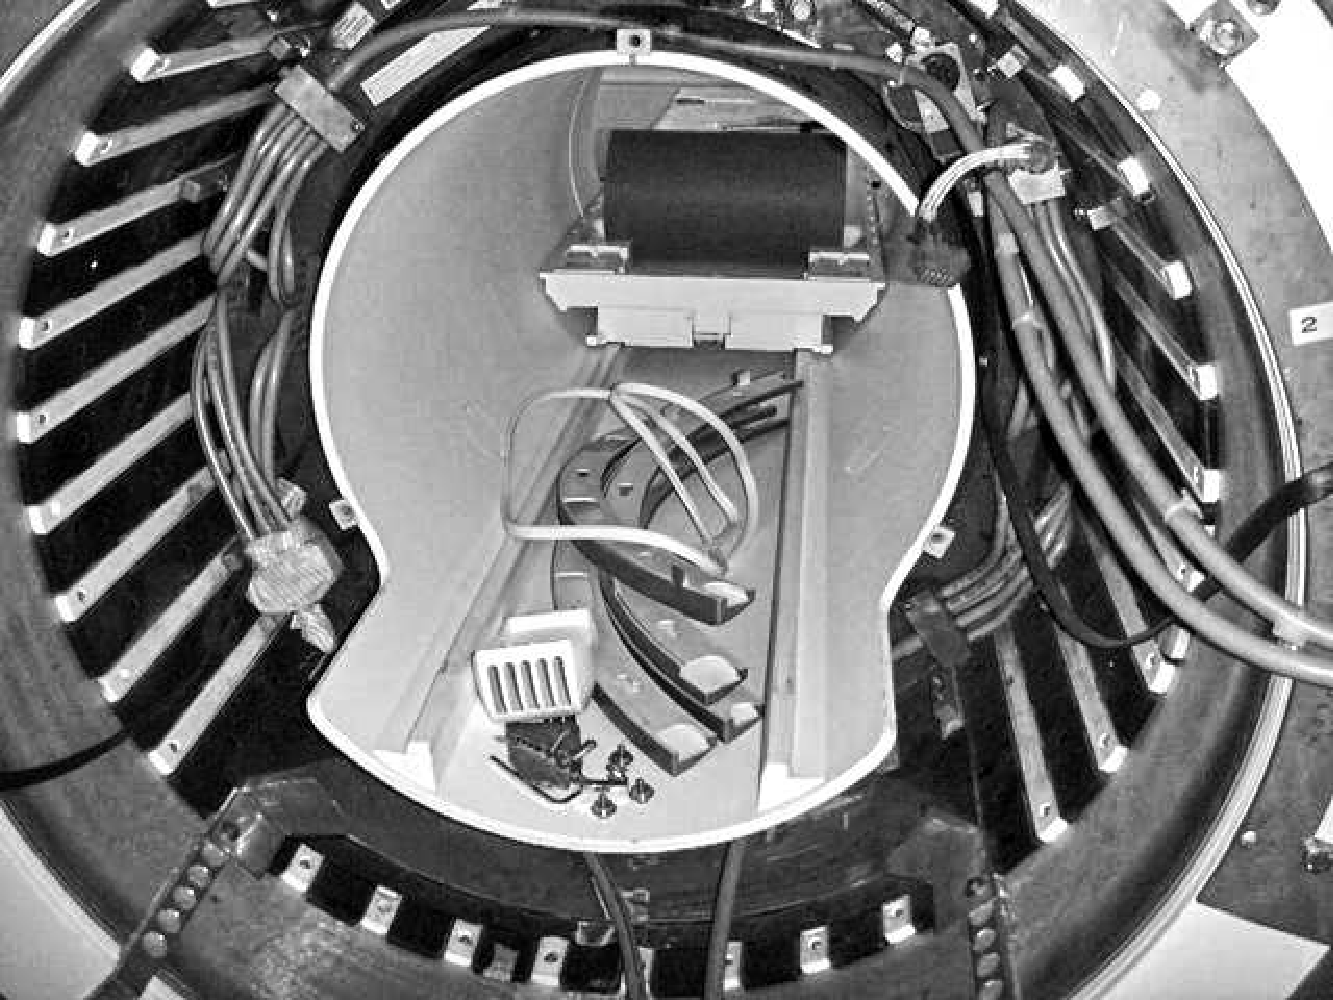
\includegraphics[width=.45\columnwidth,height=0.4\textheight,keepaspectratio]{PICT0036_bw}~
%\includegraphics[width=.45\columnwidth,height=0.4\textheight,keepaspectratio]{dsc00997}%
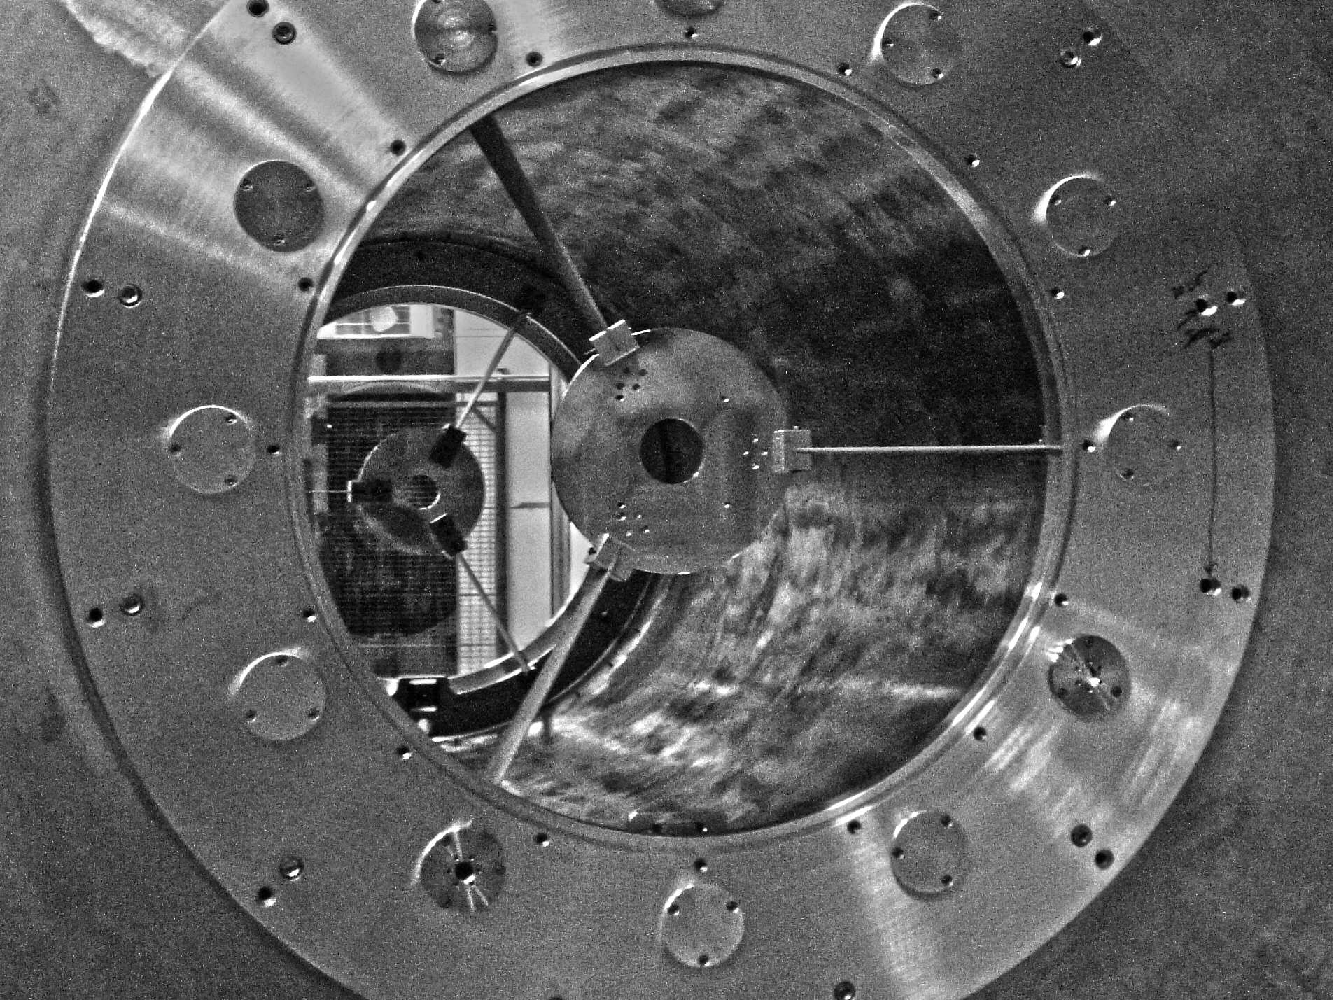
\includegraphics[width=.45\columnwidth,height=0.4\textheight,keepaspectratio]{dsc01224}%
\caption[The ``Patient End'' of the HELIOS solenoid before and after conversion to a spectrometer]{The ``Patient End'' of the HELIOS solenoid before and after conversion to a spectrometer; (left) showing MRI scanning hardware, and (right) showing the large adapter flange and alignment ``spider''. Photo (left) by B.~B.\ Back, \photodate\formatdate{6}{11}{2006} }%
\label{MRI}%
\end{figure}

For use as a nuclear spectrometer, the hardware associated with MRI scanning had to be removed (see Fig.~\ref{MRI}).  Stripped of scanning hardware, the interior diameter of the solenoid bore is 92.5\,cm and 234.7\,cm in length.  Based on sonic measurements, the solenoid wall was determined to be 5.3\,mm thick.  With the interior hardware removed, the bore-surface of the solenoid was polished to make it suitable as a vacuum chamber.  The ends of the solenoid featured square-faced mounting faces for annular field shims%called --- look up in users manual
.  These mounting faces permitted the entire solenoid volume to be converted to a vacuum vessel by sealing the ends of the bore with large-opening aluminum adapter flanges% mounted to either end of the solenoid
.

Each adapter flange has an opening diameter of 71.12\,cm and features twelve 4.45\,cm diameter feedthroughs.  These feedthroughs are used for a variety of functions as described throughout the following chapters, including detector signals.  An additional removable flange reduces the opening to mate with a 20\,cm diameter beam-line pipe.  This flange features four 16.51\,cm diameter feedthroughs.  A 20\,cm beam pipe is used for HELIOS instead of the ATLAS-standard 10\,cm beam pipe to aid in vacuum pumping.  All of the hardware in the immediate vicinity of the magnet is constructed from non-\-magnetic materials---primarily aluminum alloys and 316 stainless steel.  A photograph of the HELIOS solenoid, fully converted for use as a spectrometer, appears in Fig.~\ref{solenoid}.

\begin{figure}
\centering
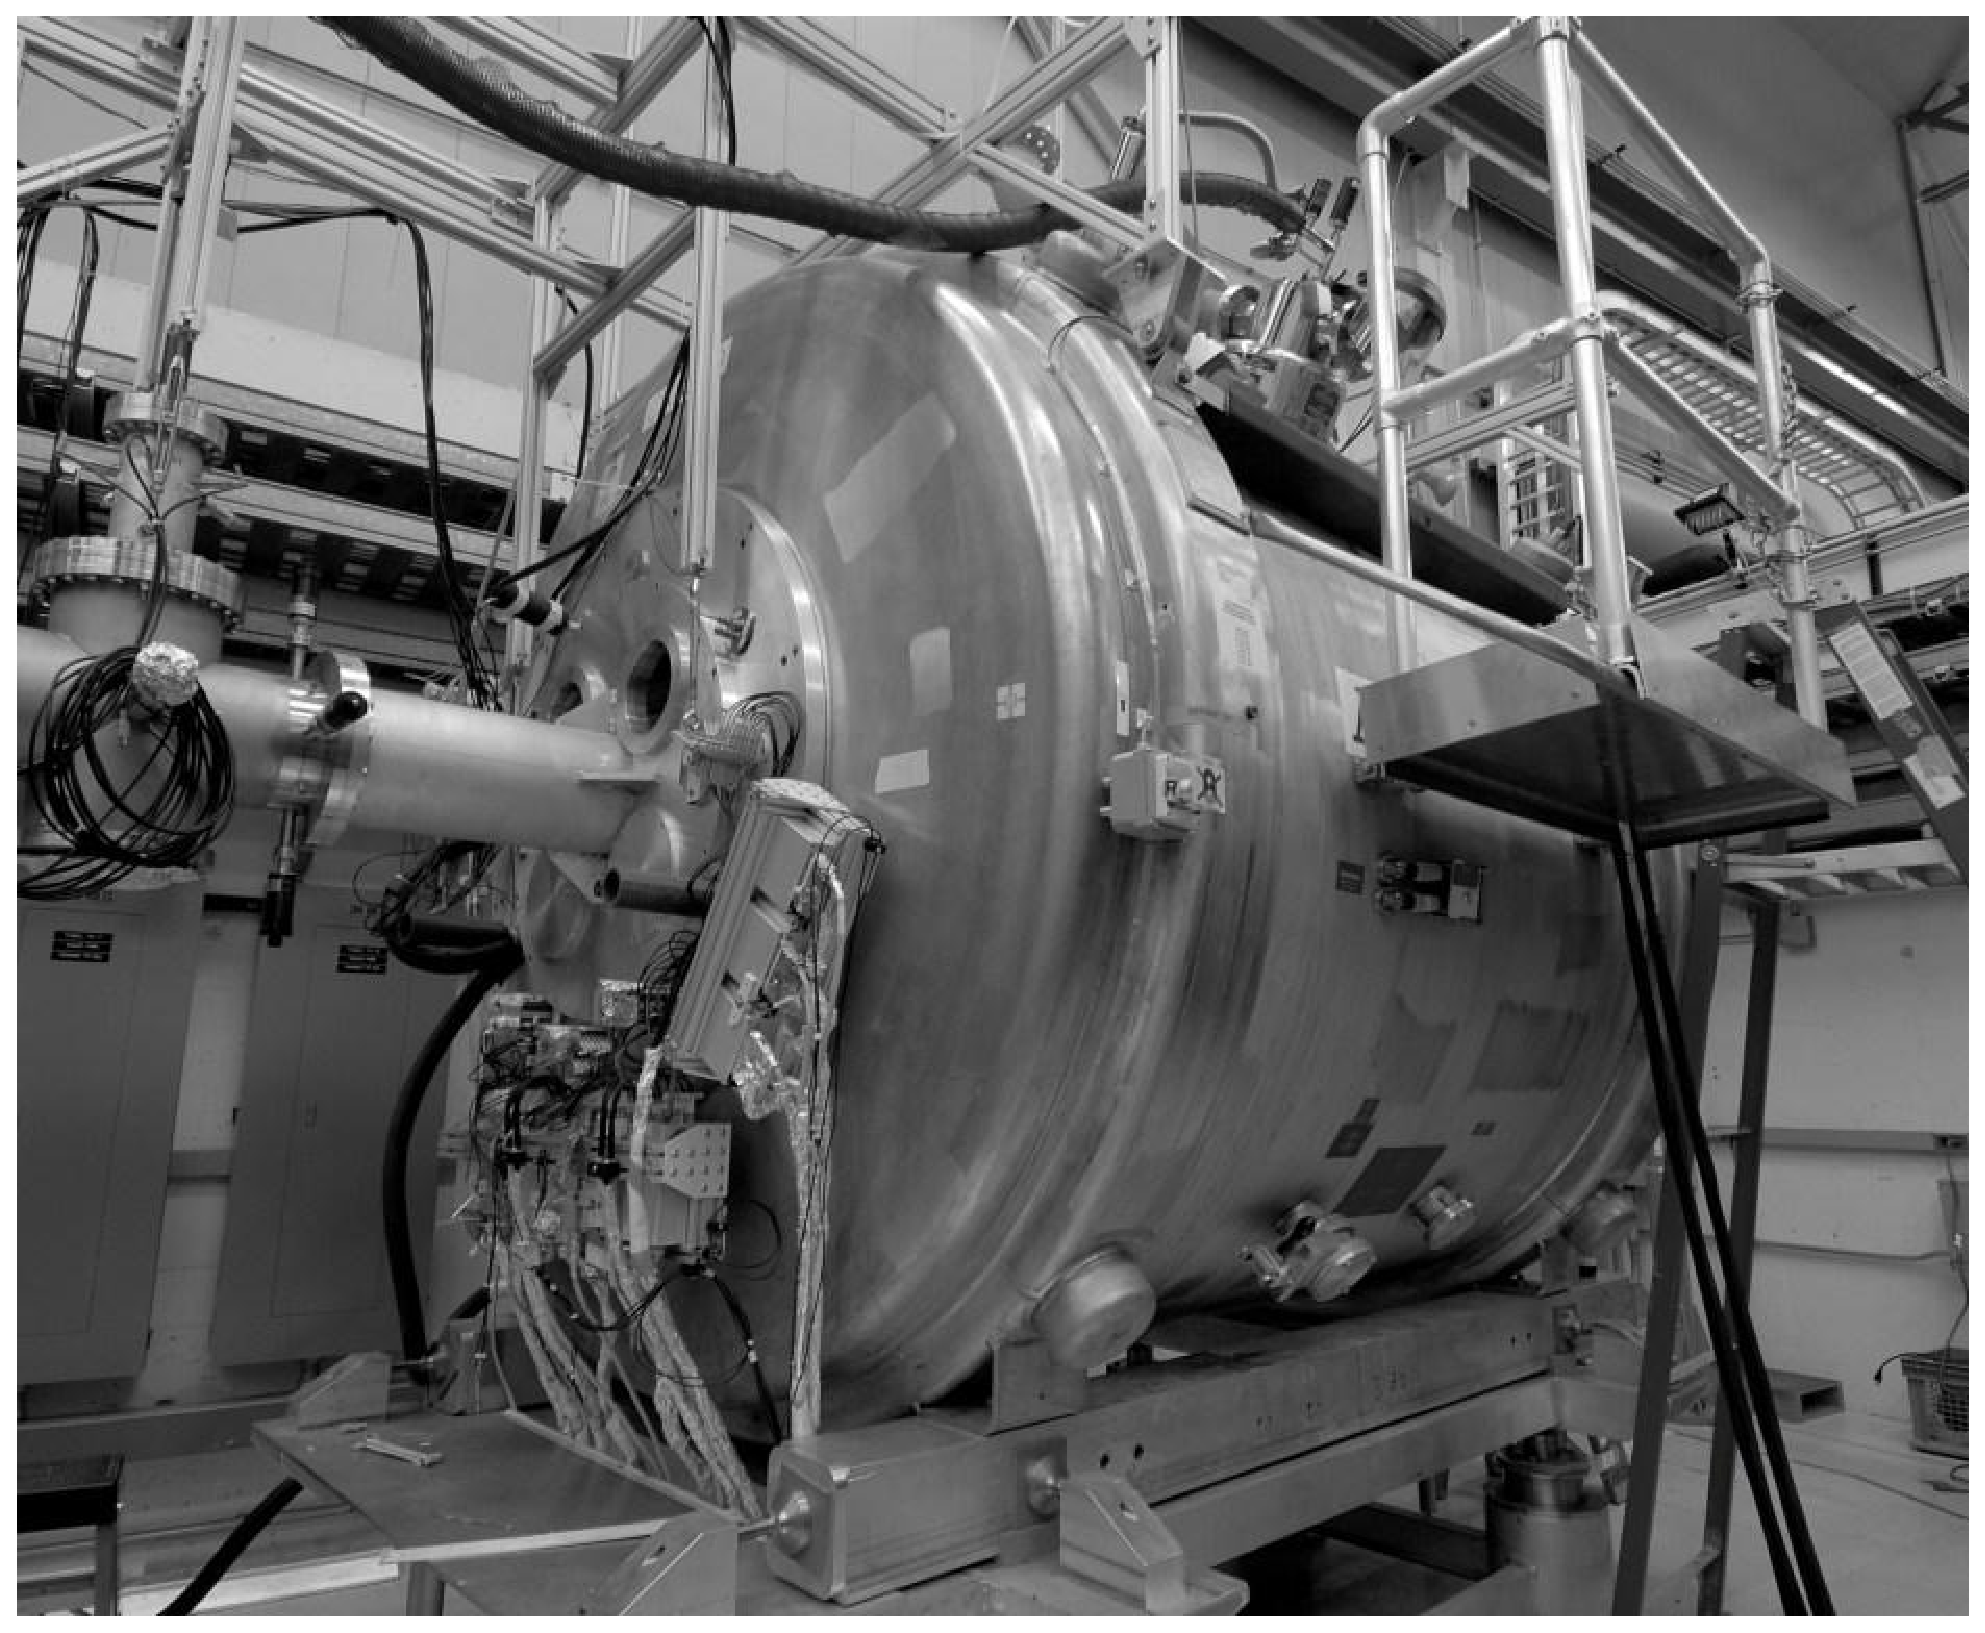
\includegraphics[width=\linewidth,height=0.4\textheight,keepaspectratio]{../NIM_Paper/Figures/DSC_0792_compressed}
\caption[The HELIOS spectrometer as installed at the ATLAS accelerator]{The HELIOS spectrometer as installed at the ATLAS accelerator.  Beam enters from left.  The preamplifers are mounted to the bottom and lower right-hand side of the 115\,cm diameter sealing flange.  Photo by A.~H. Wuosmaa, \photodate\formatdate{15}{3}{2010}.  This figure also appears in Ref.~\cite{Lighthall_2010}.}
\label{solenoid}
\end{figure}

\section{Field Map}
Particle trajectories calculated analytically, such as those presented in Chapt.~\ref{HELIOS_Concept}, assume a purely axial, uniform magnetic field.  Such a field is produced by an ``ideal'' solenoid of infinite length.  However, a realistic solenoid of finite length will produce a magnetic field with systematic non-\-uni\-for\-mi\-ties.  To account for the effects of such non-uniformities, the non-uniformities can be modeled, as in Ref.~\cite{Wuosmaa_2003}, or the field map of an existing magnet can be used, as in Ref.~\cite{Wuosmaa_2007}.  In order to assess and characterize the HELIOS solenoid, a map of the magnetic field was made in October, 2007.
%\subsection{Measurement}
\subsection{Equipment}
The components of the magnetic field were measured using an F.~W. Bell Model ZOA73-3208 three-axis Hall probe.  The probe was read out via an F.W. Bell Series 9900 Gaussmeter.  The probe consisted of an aluminum rod, 20\,cm long and 0.79\,cm in diameter, mounted in a plastic handle with the Hall probe sensors near the tip of the rod (see Fig.~\ref{probe}).  The Hall plates within the probe had a stated mutual perpendicularity of $\pm 2^\circ$. Both pieces of hardware were used in a previous application.  

Measurements were read out passively with the gaussmeter in ``master'' mode by a purpose-written program using LabVIEW\texttrademark.  Throughout the field measurements the gaussmeter was kept in a region of low magnetic flux ($<500$\,$\mu$T) while extension cables allowed the probe to be moved throughout the solenoid volume.  The gaussmeter had a stated DC resolution accuracy of $\pm0.035$\%.  For example, 0.01\,$\mu$T (1\,mG) resolution at a field of 300\,$\mu$T (3\,G) and 100\,$\mu$T (10\,G) resolution at 3.0\,T.  The probe was calibrated for probe and circuit offset errors by placing the probe in the gausmeter's 80\,dB attenuation shielded ``zero gauss'' chamber.
 
After considering a variety of probe jig designs, such as an articulating arm on a cart, it was decided to mount a rotating probe jig to the flange faces of the solenoid. %, as shown in Fig.~\ref{MRI}.
  This approach was chosen to provide reproducibility in measurement position by having the probe jig mounted to the solenoid and to take advantage of the cylindrical symmetry of the solenoid.   In this configuration, the three measured components corresponded to the axial ($\vec{\mathscr{B}}\cdot\hat{z}$), radial ($\vec{\mathscr{B}}\cdot\hat{\rho}$), and azimuthal ($\vec{\mathscr{B}}\cdot\hat{\phi}$) components of the magnetic field.
\begin{figure}%
\begin{center}
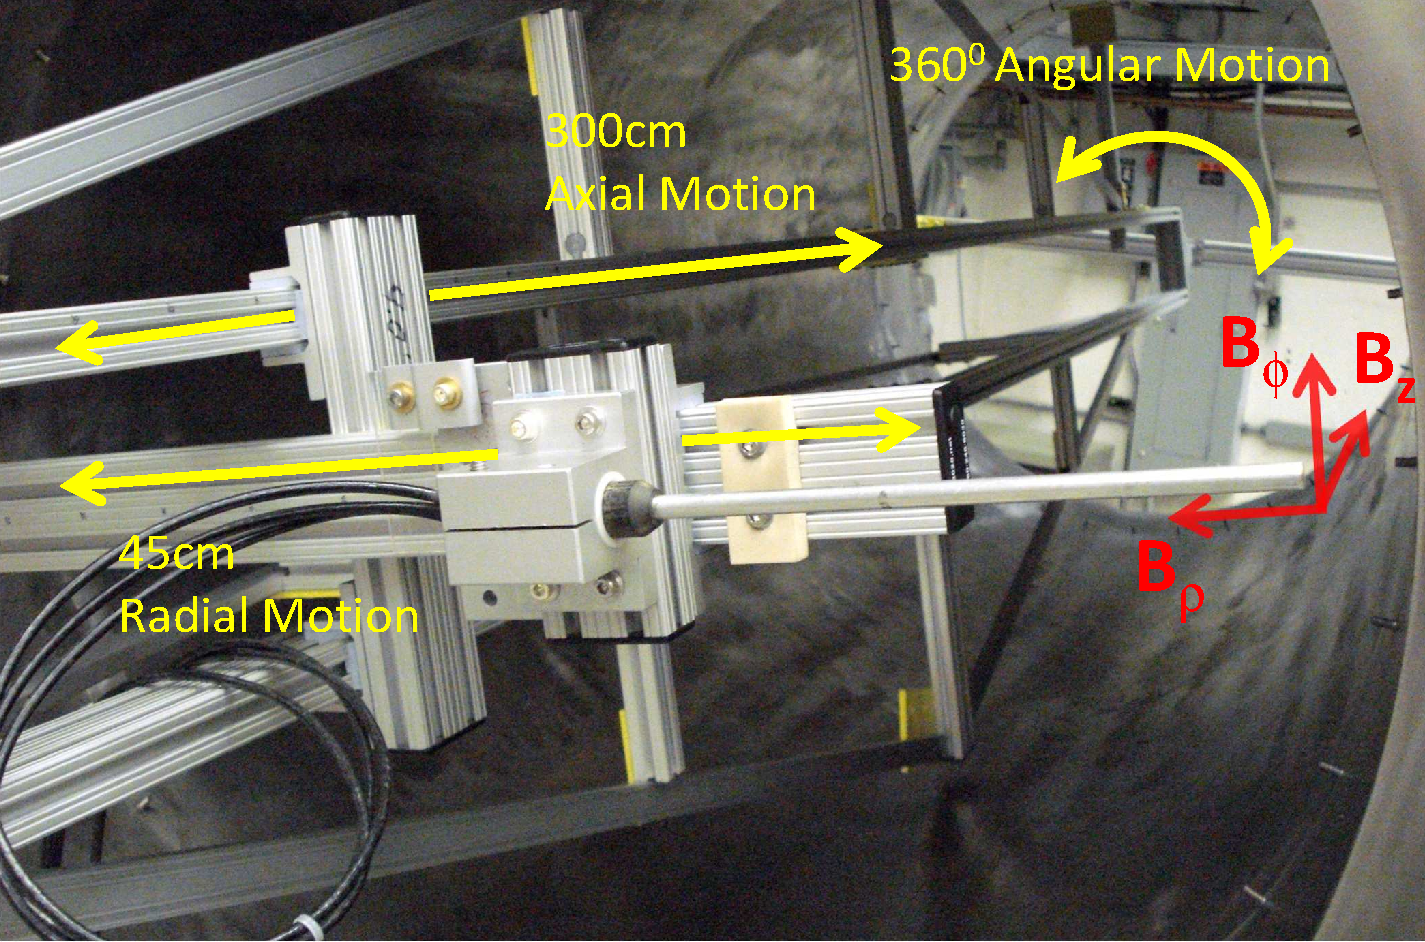
\includegraphics[width=\columnwidth, height=0.38\textheight,keepaspectratio]{probe3}%	
\end{center}
\caption[Hall probe mounted in the field mapping jig within the solenoid volume]{Hall probe mounted in the field mapping jig within the solenoid volume.  The probe jig is design so that the tip of the Hall probe rotates along a path concentric with the solenoid bore At each combination of axial position and angle, the probe translates along the radius of the solenoid.}%
\label{probe}%
\end{figure}

\subsection{Alignment}
Two parallel rails ran the length of the solenoid axis, allowing the probe to move on linear bearings over a range of $-175.85\leq z \leq +114.15$\,cm, relative to the mechanical center of the solenoid (the solenoid itself covering a range of $\pm117.35$\,cm).  The axial rails of the probe jig straddled the mechanical axis of the solenoid such that the probe could travel along a radial path, thus sampling the field along the solenoid axis ($\rho = 0$).  Due to the great length of the axial rails, the probe jig had to be structurally reinforced.  Trusses were added to the axial rails to increase their rigidity and minimize sagging.

The field probe was oriented with the body of the probe aligned radially, with the tip of the probe pointing outward.  With the trusses in place, the probe was aligned to rotate in a circular path, concentric with the rim of the flange faces to within 0.5\,mm.  The radial and axial rails were graduated every 5\,cm~$\pm 0.5$\,mm for linear measurement reproducibility.  Each downstream end of the magnet (shown in Fig.~\ref{MRI}) had screws protruding from the solenoid bore every 10$^\circ$.  These screws were used as reference points (and anchors) for measurements made at different rotation angles.

The design iteration shown in Figs.~\ref{MRI} and~\ref{probe} featured two linear bearings connecting the central carriage of the jig to the axial arms.  Measurements made with this configuration showed 100+\,G variations and discontinuities through central region of the solenoid where the field is expected to be uniform.  It was determined that these variation were due to the radial arm of the probe jig pivoting in place.  This design was later upgraded to six anchoring points on the axial rails, keeping the radial arm of the jig rigidly perpendicular to the axial rails.  The reinforcement of the radial arm eliminated the apparent variations in the axial field.

Within the tip of the probe, the Hall plate sensors had to be aligned to the mechanical axes of the solenoid. The method by which the probe was aligned within the jig is illustrated in Fig.~\ref{probe_align}.  The tip of the probe was placed within 1\,cm of center of the solenoid.  Then the probe was then oriented within the jig to maximize the reading on the ``axial'' Hall probe.

\begin{figure}%
\centering
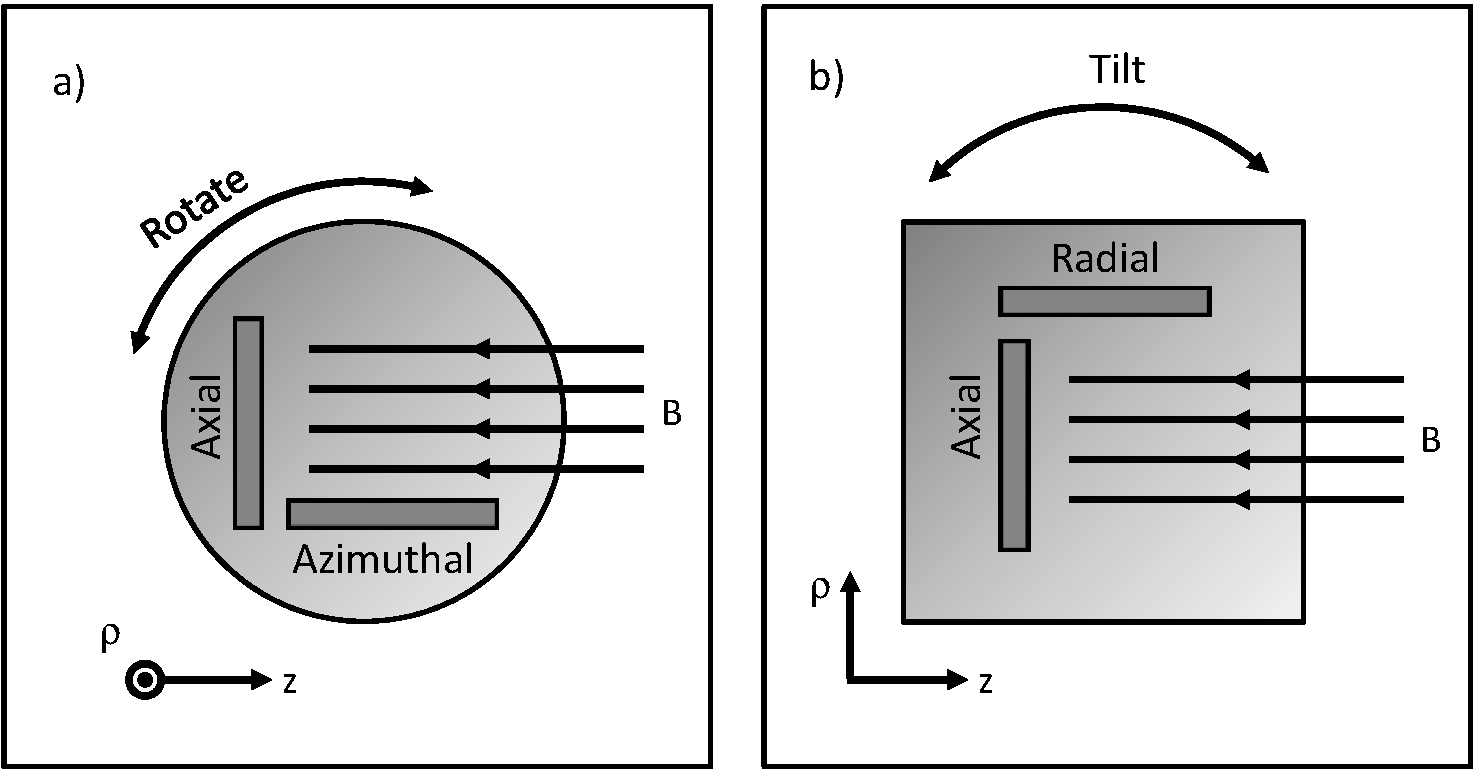
\includegraphics[keepaspectratio,height=0.5\textheight,width=\columnwidth]{probe_align}%
\caption[Illustration of the method of alignment of the 3-axis Hall probe]{Illustration of the method of alignment of the 3-axis Hall probe.  The magnetic field is directed right to left in both figures.  The probe is aligned by a) rotating the probe along its radial axis to minimize the reading in the ``azimuthal'' Hall plate.  Next, b) the probe is tilted in the $\rho$-$z$ plane to minimize the reading in the ``radial'' Hall plate.}%
\label{probe_align}%
\end{figure}

\subsection{Method}
Measurements were carried out by rotating the jig with the probe at fixed $z$ and $\rho$ positions, taking a measurement every 10$^\circ$.  At each $z$ position, this process was repeated at radii every 5\,cm between 0--45\,cm, inclusive.  Thus, each cross section contains 360 data points comprised of 10 concentric circles.  A total of 59 such field cross sections were measured every 5\,cm over a range of nearly 3\,m.  The result is a magnetic field map of 21,240 points inside and outside the solenoid volume with a corresponding average measurement lattice spacing of 4.4\,cm.  An averaged and interpolated version of the field map made up of 410 points appears in Appendix~\ref{field_map_data}.
 
\section{Field Analysis}
Fig.~\ref{map} shows the results of the field mapping.  For each combination of $z$ and $\rho$, the points have been averaged over the 36 angular measurements.  Every other radius set up to $\rho=40$\,cm has been plotted for clarity.  The deviations from uniformity of the magnetic field take the form of systematic variations in the axial and radial field components of the field.    

\begin{figure}%
\centering
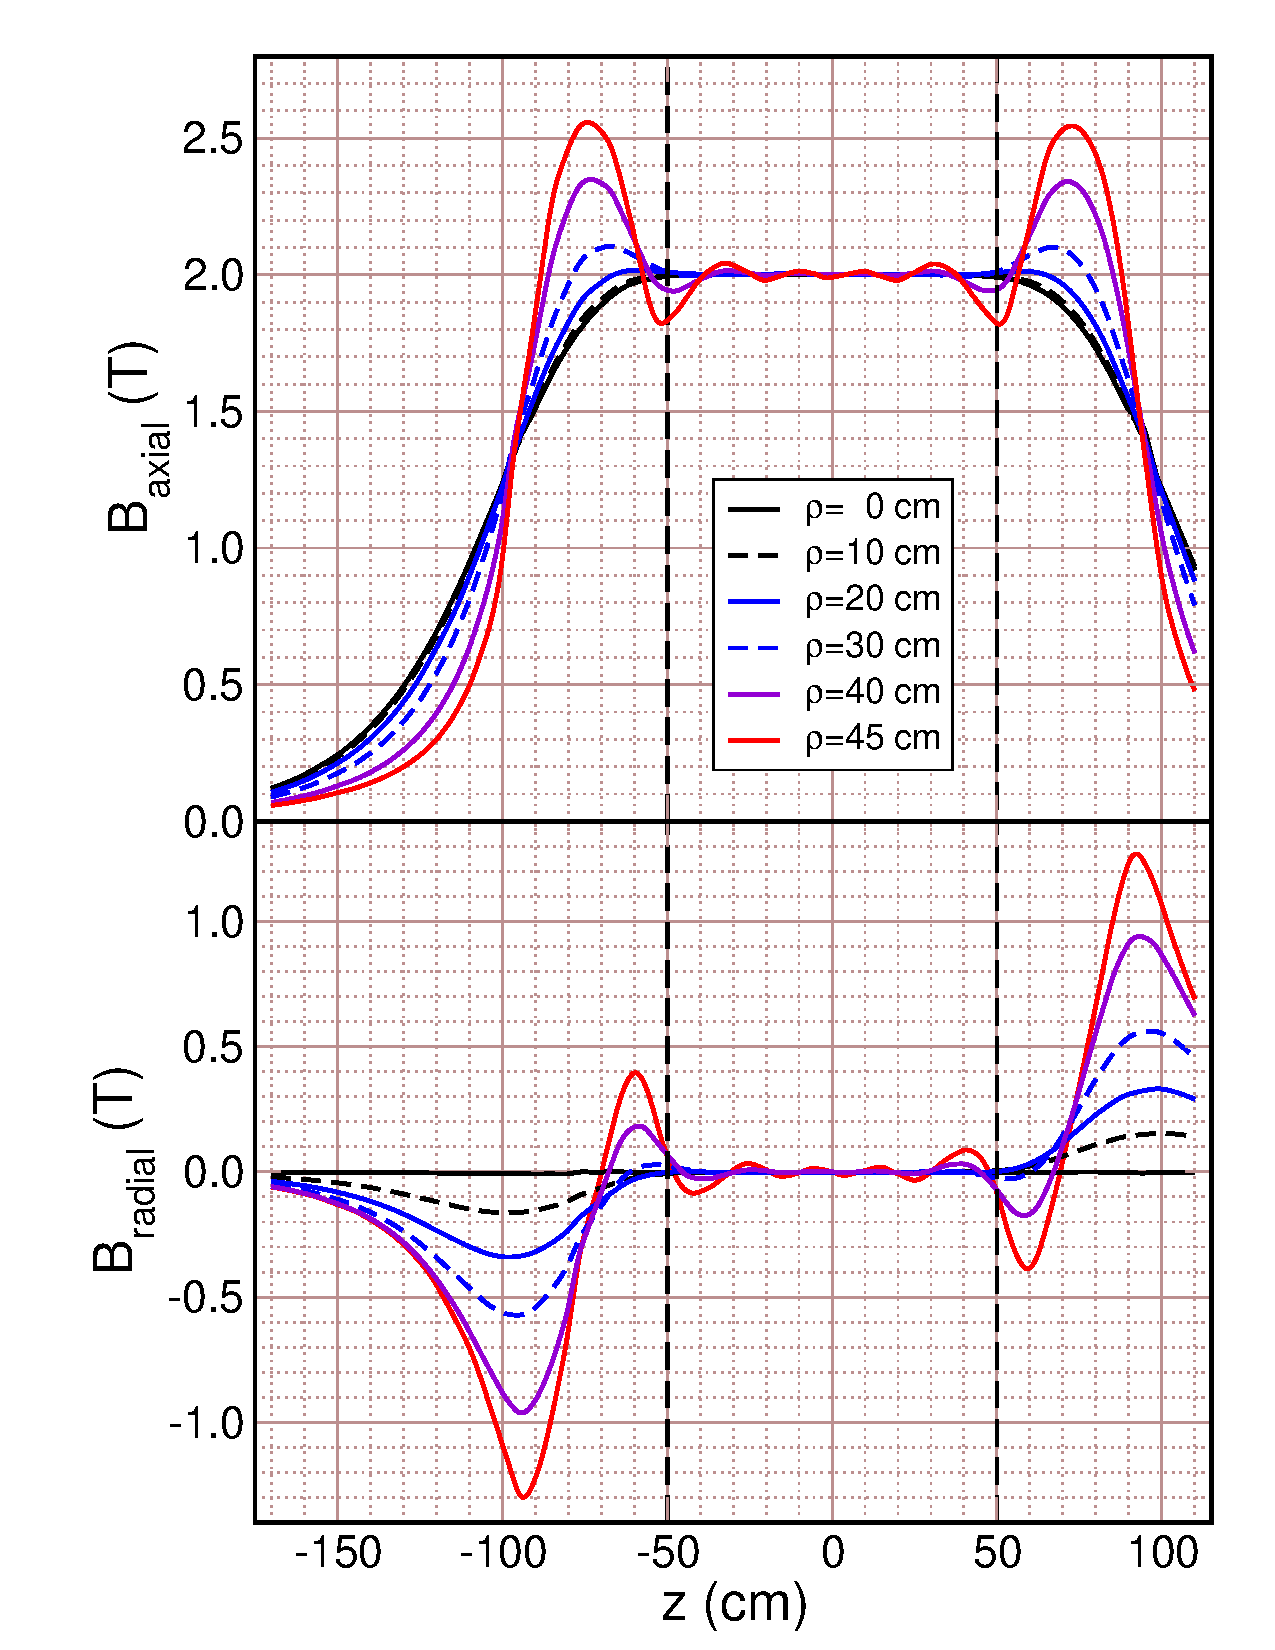
\includegraphics[keepaspectratio,height=0.9\textheight,width=\columnwidth]{field_map_45}%
\caption[Field map of the HELIOS solenoid]{Field map of the HELIOS solenoid.  The axial and radial field components are plotted with a spline fit to the measured values as a function of axial position for five different radii.  The vertical dashed lines indicate the fiducial cylindrical volume.}%
\label{map}%
\end{figure}

\subsection{Gross Structure}
\subsubsection{Axial}
The structure of the magnetic field is consistent with that produced by a 6-coil superconducting solenoid with a 2-coil active shield~\cite{Montgomery_1969}.  This is the structure which is presented schematically in the solenoid service manual.  The effect of these coils is evinced by the 6 peaks and 2 prominent troughs in the $\rho=45$\,cm axial field map in Fig.~\ref{map}.  The axial field is symmetric to within the precision of the measurements about a point offset -0.5\,cm from the mechanical center of the magnet.  This symmetry is demonstrated in Fig.~\ref{axial_reflect}.  The ``kink'' in the axial field at about $z= \pm95$\,cm from the center is consistent with two concentric solenoids with opposite current~\cite{Montgomery_1969}.

\begin{figure}%
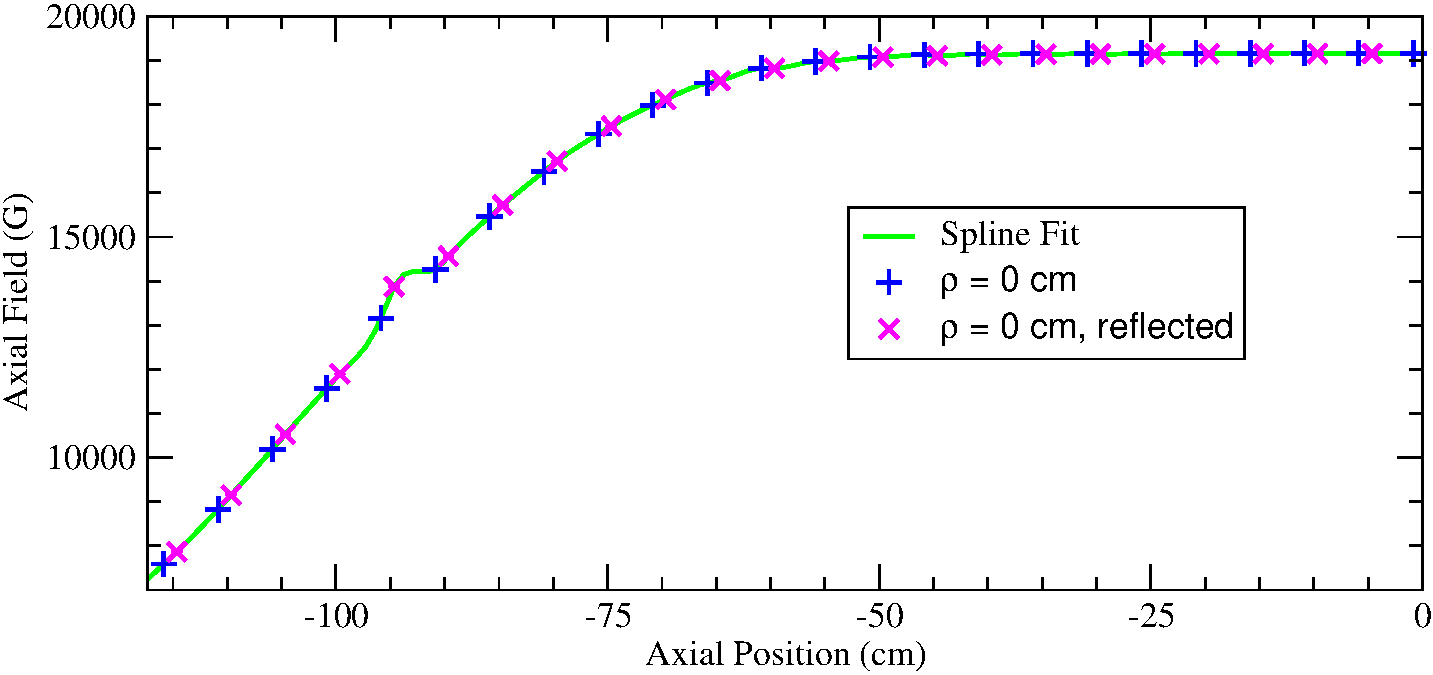
\includegraphics[width=\columnwidth]{axial_fit}%
\caption[Symmetry of the axial field component over the interior of the solenoid]{Symmetry of the axial field component over the interior of the solenoid. The upstream axial field has been reflected about $z=-0.5$\,cm.  The combined points have been fit with a spline fit.  Error bars on position and field are on the order of the line thickness.  }
\label{axial_reflect}%
\end{figure}

On the solenoid axis, the axial field falls to 10\% of its central value at approximately $z= \pm150$\,cm from the center of the magnet and to 0.1\% at approximately $z= \pm230$\,cm from center.  At distances greater than 175\,cm from the center of the magnet, the fringe field is well approximated by an inverse-cubic function ($\mathscr{B}_z\approx 1/z^3$).  The south pole of the average axial magnetic field corresponds to the ``Patient End'' of the solenoid; as shown in Fig.~\ref{MRI}, this end is the downstream end of the solenoid.

\subsubsection{Radial}
Throughout the solenoid, the radial field component is well approximated by a third-order polynomial function of the cylindrical radius $\rho$.
\begin{equation}
\mathscr{B}_\rho=A+B\rho+C\rho^2+D\rho^3
\label{eq:radial}
\end{equation}
  The radial field reaches a maximum absolute value of 63\% of the central field approximately $z= \pm95$\,cm from the center of the magnet at a cylindrical radius of $\rho =45$\,cm, corresponding to the location of the fringe field reducing coils.  

\subsubsection{Tangential}
The ``tangential'' or azimuthal component of the magnetic field ($\vec{\mathscr{B}}\cdot\hat{\phi}$) was  measured to be less than 1.8\% of the total magnetic field and had an average value of 0.32\% of the total magnetic field.  Fig.~\ref{tan_field} shows a representative example of the tangential field, measured at $\rho=15$\,cm.  Included in the plot are fitted projections of both the axial and radial fields.  The results of such fits at all radii indicate that the ``azimuthal'' Hall plate sensor was $0.07^\circ \pm 0.02^\circ$ away from perpendicular, relative to the ``axial'' sensor, and $1.31^\circ \pm 0.14^\circ$ away from perpendicular, relative to the ``radial'' sensor.  The residual azimuthal component is asystematic and structureless, consistent with zero.

\begin{figure}%
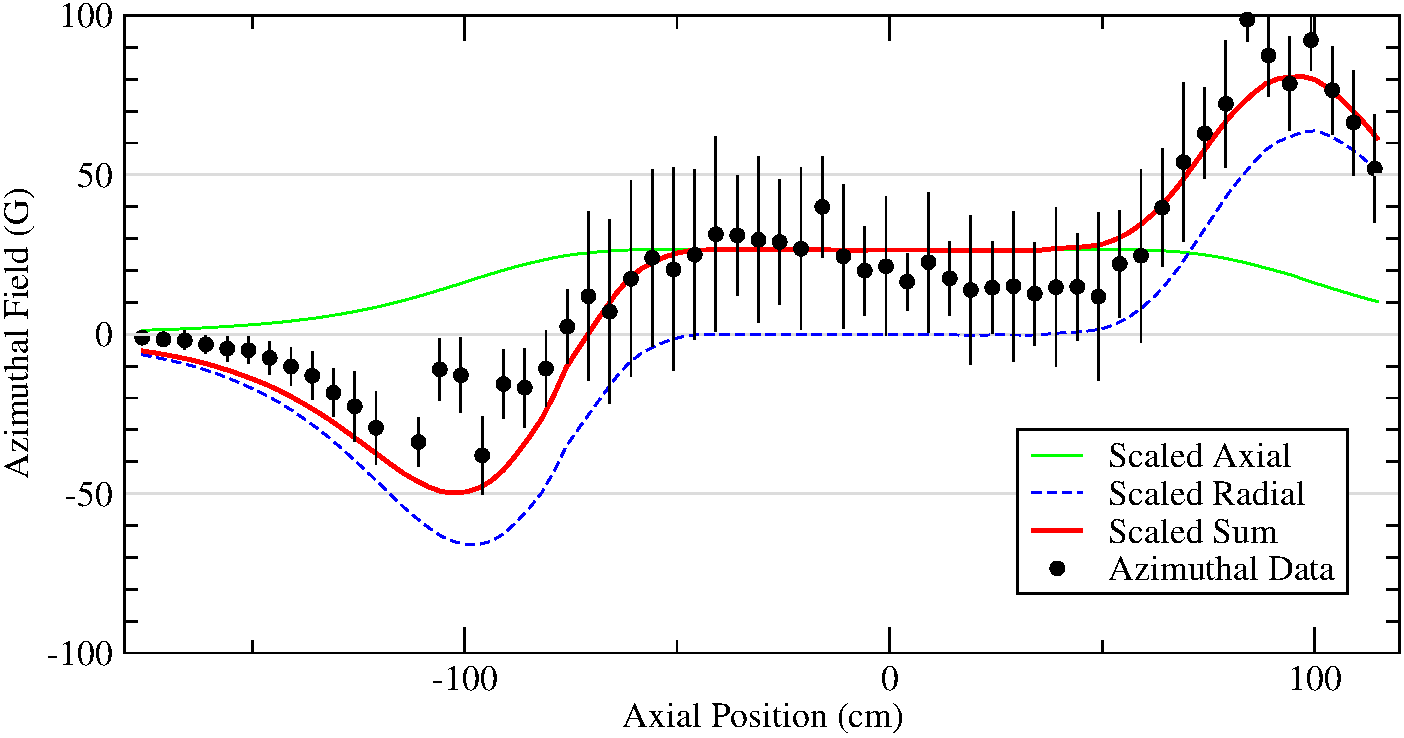
\includegraphics[width=\columnwidth]{r15_tan}%
\caption[Azimuthal  field component at $\rho=15$\,cm with projected fit of the other field components]{Azimuthal  field component at $\rho=15$\,cm with projected fits of the other field components.  Error bars of 1\,$\sigma$ are shown.  Nearly all of the points are within 1\,$\sigma$ of the scaled sum, indicating the ``azimuthal field'' is consistent with zero.}%
\label{tan_field}%
\end{figure}

\subsubsection{Uniformity}

The magnetic field is homogeneous and purely axial in a spherical field region about the geometric center of the solenoid, referred to as the Diameter Spherical Volume (DSV).  For medical purposes, similar magnets are guaranteed to have a homogeneous region (``Field of View'') 40\,cm in diameter.  
In this region, the measured variation in the magnetic field is less than the stated measurement uncertainty (0.035\%) and is consistent with zero.  In a 90\,cm DSV, which extends to the solenoid bore, the mean absolute field non-uniformity is slightly higher at 0.05\%.  
The absolute field non-uniformity increases to a maximum of 3.1\% within a central cylindrical volume 1\,m long and 40\,cm in radius.  Section \ref{simulation} describes how these characteristics define the fiducial volume of the spectrometer.

\subsection{Fine Structure}
A detailed analysis of the field map revealed systematic azimuthal variations in the measured radial field components.  An example such variations is shown in Fig.~\ref{sine_fit}.  Variations of this kind are consistent with an offset between the rotational axis of the field mapping jig and the magnetic field axis.  Fig.~\ref{map_off} illustrates how these variations may arise.  If the probe is rotated along a circular path which is offset from the magnetic field axis, a range of magnetic equipotentials are sampled.  The result would be a sinusoidal variation in the measured magnetic field as shown in Fig.~\ref{sine_fit}.

\begin{figure}%
\centering
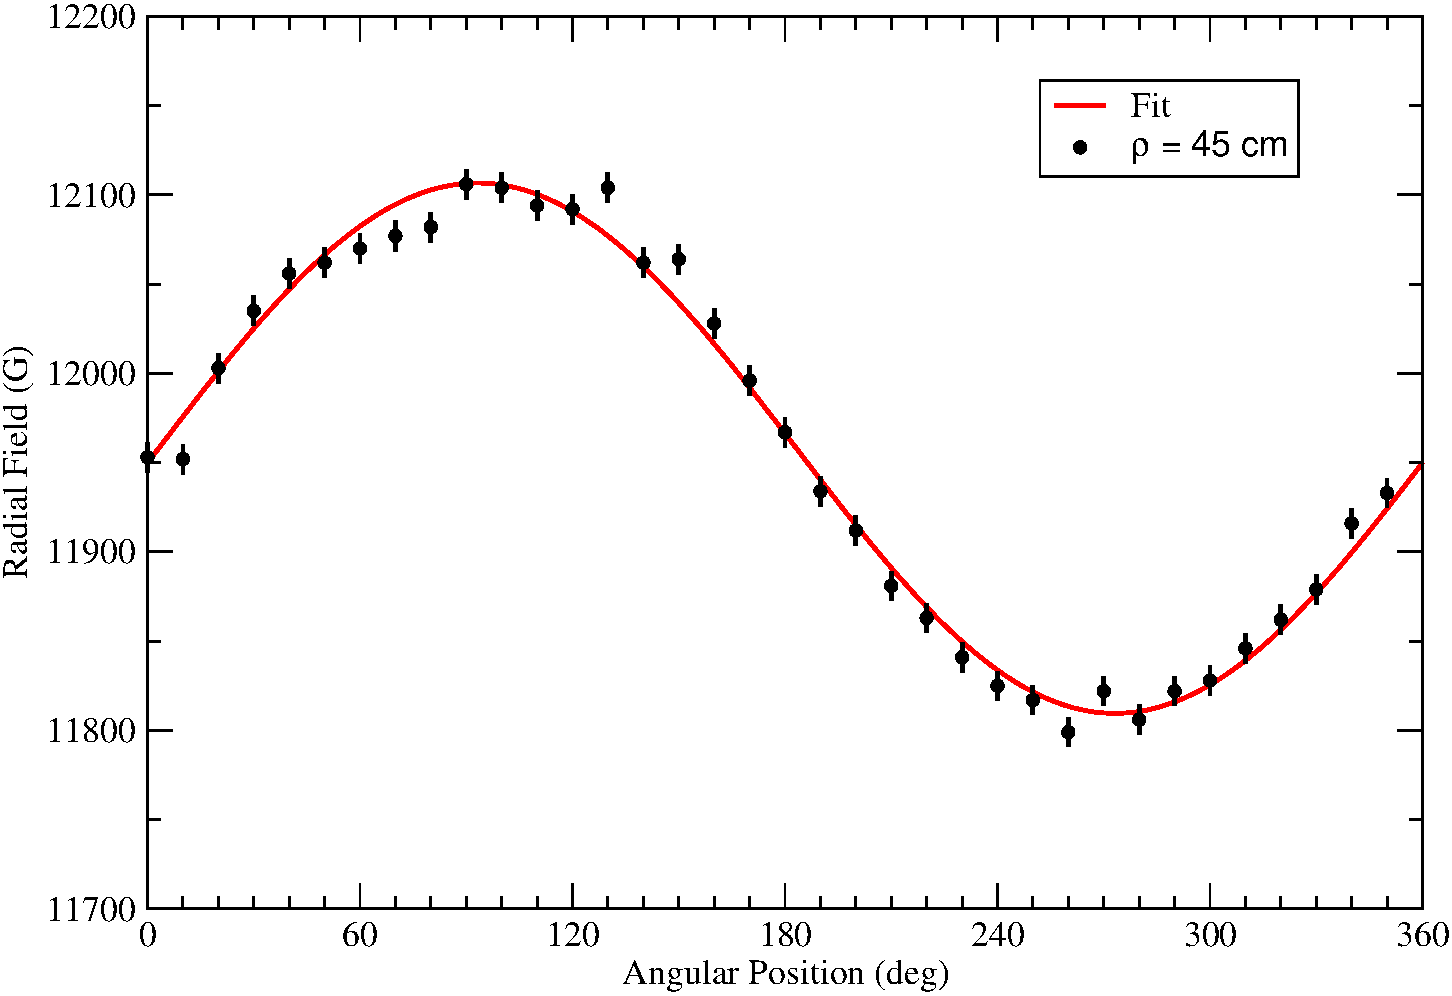
\includegraphics[width=\columnwidth,height=0.4\textheight,keepaspectratio]{sine_fit}%
\caption[Measured azimuthal variation in the radial field component at $z=94.15$\,cm, $\rho=45$\,cm]{Measured azimuthal variation in the radial field component at $z=94.15$\,cm, $\rho=45$\,cm.   $\pm 0.035$\% error bars are shown.  The data have a fluctuation of $\pm 63$\,G about the mean.  The line is a sine cure fit to the data ($\chi^2/\textrm{dof}=1.98$).}%
\label{sine_fit}%
\end{figure}

\begin{figure}%
\centering
\fbox{
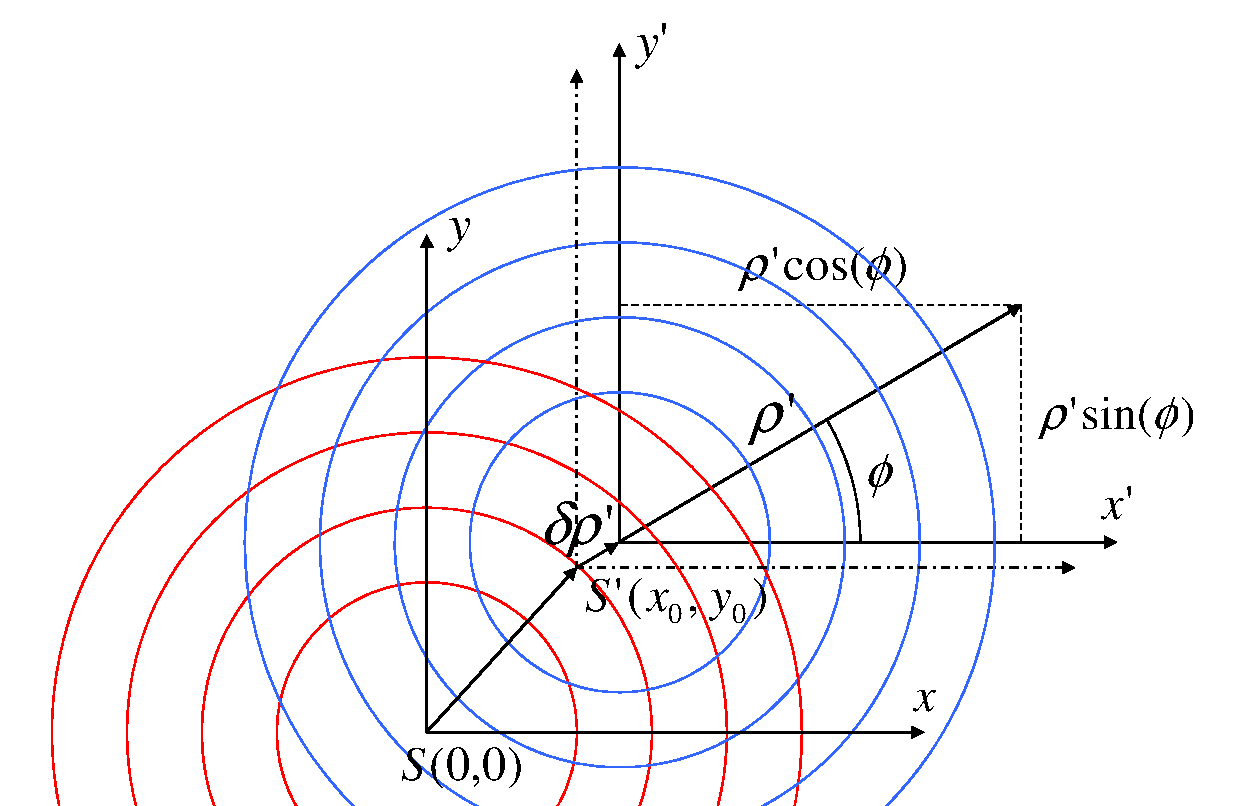
\includegraphics[width=\columnwidth,height=0.4\textheight,keepaspectratio]{map_offset3}%
}
\caption[Illustration of the source of the measured sinusoidal fluctuation in the radial field component]{Illustration of the source of the measured sinusoidal fluctuation in the radial field component.  The mechanical axis $S^\prime$ is offset from the magnetic field axis $S$.  $\delta \rho$ is a linear offset in the measured quantity $\rho$.  Adapted from Refs.~\cite{Lighthall_2008SLM,Vann_2008}.}%
\label{map_off}%
\end{figure}

Using the relationship illustrated in Fig.~\ref{map_off}, the radius relative to the magnetic axis $\rho$ can be written in terms of the measured radius $\rho^\prime$ as
\begin{equation}
\rho=\sqrt{[(\rho^\prime + \delta \rho) \cos(\phi)+x_0]^2+[(\rho^\prime + \delta \rho)\sin(\phi)+y_0]^2}
\label{rho_offset}
\end{equation}
where $x_0$ and $y_0$ are the horizontal and vertical alignment offsets, respectively, and $\delta \rho^\prime$ is a linear offset in $\rho^\prime$.  The linear offset parameter is included because the exact position of the Hall plate sensor within the tip of the probe had to be estimated from non-technical schematics.  All of the readings in the ``axial'' sensor for the measurements at $z= \pm 95$\,cm corresponded to a positive radial flux, except for those at $\rho^\prime=0$, which measured a negative flux.  Therefore, those measurements were actually sampling the field at a radius of $-\delta \rho^\prime$.  Also, since this feature was absent from the measurements at $\rho^\prime \geq 1$\,cm, the value of $\delta \rho^\prime$ must be $< 1$\,cm.

When the HELIOS solenoid was installed on the ATLAS beam line, it was aligned such that the beam path was collinear with the mechanical axis of the solenoid.  Therefore, an offset between the magnetic field axis and the mechanical axis of the solenoid could have an impact on experiments conducted with HELIOS.  To asses any possible offset, the radial field was analyzed at $z= \pm 95$\,cm, where the radial field is strongest.  In order to have a more statistically significant sample, % of the radial field at $z= \pm 95$\,cm,
 the field cross sections at those points included an additional 576 measurements, made at radius intervals of 1\,cm in the range $0<\rho<10$\,cm.  

To fit the data, the measured radius was related to the sample-point radius by Eq.~\ref{rho_offset}.  Then, the sample-point radius $\rho$ was fit with a cubic function.  For measurements made at $\phi \geq 180^\circ$, the measured radius and field were reflected about the origin to ensure a symmetric fit function.  To determine a $\chi^2$ fit value, the average value of the tangential field component (for all measurements) was used as the value of the uncertainty in the magnetic field measurement $\delta \mathscr{B}=15.4$\,G.  The results of fitting the radial field at the given cross sections is shown Table~\ref{offset_param} and Fig.~\ref{cubic_fit}.

\begin{table}
  \begin{center}
    \begin{tabular}{.....|....}
      \hline
      \multicolumn{1}{c}{\multirow{3}{*}{$z$}} &
      \multicolumn{4}{c|}{$\rho^\prime \leq 30$\,cm} &
      \multicolumn{4}{c}{$\rho^\prime \leq 45$\,cm} \\ \cline{2-9}
       &\multicolumn{1}{c}{$x_0$} &\multicolumn{1}{c}{$y_0$} &\multicolumn{1}{c}{ $\delta \rho^\prime$}&\multicolumn{1}{c|}{$\chi^2/\mathrm{dof}$}
              &\multicolumn{1}{c}{$x_0$} &\multicolumn{1}{c}{$y_0$} &\multicolumn{1}{c}{ $\delta \rho^\prime$}&\multicolumn{1}{c}{$\chi^2/\mathrm{dof}$}\\\hline \hline 
       %& $x_0$ & $y_0$ & $\delta \rho^\prime$&$X^2/\mathrm{dof}$\\\hline \hline 
      -95.85&0.26&4.30&-0.08&5.19&0.35&4.95&2.77&109.8\\
      +94.15&-0.22&-1.59&0.26&1.38&0.01&1.45&2.51&75.7\\
      \multicolumn{1}{c}{Average}& 0.02 &2.71&0.09&&0.18&3.20&2.64\\\hline
    \end{tabular}
    \label{offset_param}
    \caption[Offset parameters for two different cubic fits to the radial field at $z= \pm 95$\,cm]{Offset parameters for two different cubic fits to the radial field at $z= \pm 95$\,cm.  Values are given in mm.  For both fit ranges $x_0$ is consistent with zero and $\delta \rho^\prime$ is consistent with the required range of 0--10\,mm.}
  \end{center}
\end{table}

\begin{figure}%
\centering
\includegraphics[width=\columnwidth]{cubic_fit2}%
\caption{Radial field data for the $z=94.15$\,cm field cross section measurement with two cubic fits.}%
\label{cubic_fit}%
\end{figure}

The fits indicate that $x_0\approx0$\,mm and $y_0\approx3\,$mm.  This may represent an actual offset in the mechanical structure of the solenoid.  However, the magnitude of the fitted value of $y_0$ is greater for the measurement at $z=-95$\,cm.  This measurement point was nearly 1\,m away from the point where the probe jig was suspended.  It is possible that despite the reinforcement from the trusses, the axial rails of the probe jig were sagging and this is the cause of the vertical offset.  The effect of a genuine mechanical offset is discussed in Chapt.~\ref{simulation}.  Finally, the linear offset is in the range $0<\delta \rho^\prime<1$\,cm, as required by the flux inversion present only in the measurements at $\rho^\prime = 0$.

%Since the bore of the solenoid---and presumably, the solenoid itself---are circular, an asymmetric 
Accounting for the eccentric rotation of the rotation of the probe jig effectively eliminates the azimuthal dependence of the radial field component for smaller radii ($\rho^\prime \leq 30$\,cm).  For larger radii, this correction still leaves a residual variation.  However, the residual azimuthal variations in the radial field components are on the order of 0.5\%, and scales roughly with the axial field component, which is consistent with a trivial non-perpendicularity of the Hall plate sensors.

\subsection{Determining the Absolute Field}
\label{absf}
The field mapping was conducted with a current of 363.00\,A in the solenoid coils.  This value was chosen to achieve a 2.00\,T field based on the field-to-current ratio given in the solenoid service manual as shown in Table~\ref{current}.  A field of 2\,T (20,000\,G) was selected in order to comply with safety guidelines, specifically, the whole body exposure ceiling limit value (TLV-C) as suggested by the American Conference of Governmental Industrial Hygienists (ACGIH).  However, the initial result of the field mapping indicated a central field of 1.9159\,T.  This measured value corresponds to a different field-to-current ratio, as shown in Table~\ref{current}.

\begin{table*}
\begin{center}
\begin{tabular}{rccc.}
\hline
Source&$\mathscr{B}_0$ Field (g)&Current (A)& Ratio (g/A)&
\multicolumn{1}{c}{Slope (keV/mm)}\\\hline \hline
Service Manual&30000&543.96&55.15&10.124\\
Field Map&19159&363.00&52.78&9.698\\\hline
\end{tabular}
\label{current}
\caption[Field-to-current relations for the HELIOS solenoid]{Field-to-current relations for the HELIOS solenoid.  Values are based on the magnet specifications given in the solenoid service manual and the results of the field map.  Also shown is the expected slope of the kinematic loci from the $d$($^{28}$Si,$p$)$^{29}$Si reaction.}
\end{center}
\end{table*}

This discrepancy introduces a dilemma: either the solenoid's field response is nonlinear or the field mapping measurements are systematically inaccurate.  To address this issue, the magnetic field was measured by a one-dimensional Hall probe at a fixed representative point on the flange face during the process of energizing the solenoid. The results of this measurement are shown in Fig.~\ref{field_lin}.  It is clear from this figure that the field response is indeed linear with current.  However, it is also clear from the self-consistent nature of the field mapping data that whatever systematic error is present effects all of the data points equally.  The conclusion is then that the measured field map quantities are 95.8\% of the actual value.

\begin{figure}[t]
\centering
\includegraphics[keepaspectratio,height=0.5\textheight,width=\columnwidth]{Field_Linearity}%
\caption[Field linearity as measured during a solenoid-energizing procedure]{Field linearity as measured during a solenoid-energizing procedure.  Measurements were made at the flange face of the HELIOS solenoid during a ramp-up to 363\,A.  The red line is a linear regression fit to the data.}%
\label{field_lin}%
\end{figure}

This conclusion is further supported by an analysis of the data from the first reaction measured with HELIOS.  For a given reaction and bombarding energy, Eq.~\ref{slope_calc} gives the expected slope of the kinematic loci based on the (uniform) magnetic field.  Fig.~\ref{badslope} shows data from three different position settings that have been shifted to line up with calculations for the two possible field strengths.  The calculations for $\mathscr{B}_0=1.91$\,T clearly do not line up with the data, while the calculations for $\mathscr{B}_0=2.00$\,T are in good agreement.

An additional implication of understanding the field-to-current ratio of the HELIOS solenoid is the maximum field setting.  The HELIOS solenoid is rated as a 3.0\,T magnet; this field value is achieved with a solenoid current of 543.96\,A, as shown in Table~\ref{current}.  However, the Siemens Model 3600 Magnet Power Supply used to energize the HELIOS solenoid will only output 518.00\,A to the solenoid.  This corresponds to a maximum possible central field value for the HELIOS solenoid of 2.8568\,T.\footnote{The value reported in Ref.~\cite{Schiffer_2010} (2.7\,T) is off by a factor of 95.8\%, which is the value based on the field map.}  This maximum field value corresponds to  a length parameter of $\mathscr{B}\rho=1.32$\,T$\cdot$m and a radial parameter of $\mathscr{B}L=6.70$\,T$\cdot$m, exceeding the requirements put forth in Ref.~\cite{Wuosmaa_2007}.

\begin{figure}%
\centering
\includegraphics[width=\columnwidth,height=0.4\textheight,keepaspectratio]{cShift_191_bw}\\
\includegraphics[width=\columnwidth,height=0.4\textheight,keepaspectratio]{cShift_200_bw}%
\caption[Determination of the absolute field by slope analysis]{Determination of the absolute field by slope analysis.  Calculated proton energies (fine dashed lines) are overlaid on two analyses of the same data set.  The data have been shifted in $z$ to best fit the calculations for $\mathscr{B}_0=1.91$\,T (top) and $\mathscr{B}_0=2.00$\,T (bottom).  In the top figure, note that the calculations overestimate $E_\mathrm{lab}$ at low energy and underestimate $E_\mathrm{lab}$ at high energy, indicating a mis-match in slope ($\mathscr{B}$-field).  In the lower figure, the data and calculations are aligned, supporting the conclusion that the field strength was indeed $\mathscr{B}_0=2.00$\,T.  In each panel, pairs of vertical lines indicate detector positions and bold dashed curves indicate the (calculated) acceptance limits.  The upper limit occurs above the axis limit in the lower figure.}%
\label{badslope}%
\end{figure}
\chapter{The Silicon Detector Array}
In order to take advantage of the HELIOS concept, the light ion reaction products transported through the HELIOS solenoid must be detected in a slender array close to the beam axis.  The radial extent of the array should be on the order of 1\,cm.  For rearward hemisphere operation, the array must also be hollow to permit the transmission of the beam to the target foil.  The silicon detectors which  make up the array must be position sensitive along their length with a position resolution on the order of $\delta z = 0.5$--1.0\,mm~FWHM.  In addition, the intrinsic detector energy resolution should be on the order of $\delta E_\mathrm{lab} =25$--50\,keV~FWHM.  This chapter describes characterization and construction of the silicon detector array as they relate to these design requirements.
\section{The Detectors}
\label{detectors}
\subsection{Specifications}
The prototype array utilizes detectors that were manufactured by Canberra Industries.  The detectors were designed for and used in a previous application as a nuclear reaction calorimeter~\cite[pp. 100--104]{Blumenthal_PhD}.  The detectors are position-sensitive passivated implanted planar silicon detectors.  The detectors are 12\,mm $\times$ 56\,mm silicon wafers, $700\pm15$\,$\mu$m thick\footnote{Thickness quoted in private communication from the manufacturer.} with active areas 9\,mm $\times$ 50.5\,mm.  The particle energy which this detector thickness is capable of stopping is shown in Table~\ref{srim} for a number of light ions.

The construction of the detectors follows the standard fabrication method of passivated implanted planar silicon detectors~\cite{Kemmer_1984}.  First the edges of the silicon wafers are passivated by thermal oxidation which, after etching, produces an insulating boundary of SiO. Next the front of each detector (the side shown in Fig.~\ref{pcb}) is implanted with boron ions to form a p$^+$n junction and the back of the detectors is implanted with arsenic to form an n-type junction.  Then after annealing, aluminum contacts, discussed below, are patterned on either side of the detector for electrical connections.  The thin layer of boron provides position sensitivity along the length  of the detector by resistive division.  The dead layer introduced by the ohmic contact on the back of the detector---typically the entrance window---is equivalent to a silicon thickness of $<50$\,nm.  The dead layer on the junction side is $<100$\,nm silicon equivalent.  A typical detector is fully depleted at a reverse-bias voltage of 190\,V producing nominal leakage current of 350\,nA.

\begin{table}
  \begin{center}
    \begin{tabular}{c..}
      \hline
      \multicolumn{1}{c}{\multirow{2}{*}{Nucleon}}  &
    	\multicolumn{2}{c}{Incidence Angle}\\ \cline{2-3}
    	&\multicolumn{1}{c}{$\vartheta=0^\circ$}&\multicolumn{1}{c}{$\vartheta=45^\circ$}\\\hline \hline 
      $p$&9.9&12.1\\
      $d$&13.2&16.2\\
      $t$&15.7&19.2\\
      $^3$He&35.1&42.9\\
      $\alpha$&39.6&48.7\\\hline
    \end{tabular}
    \label{srim}
    \caption[Stopping power calculations for the HELIOS silicon detectors]{Stopping power calculations for the HELIOS silicon detectors.  Approximate light ion energies in MeV with stopping ranges of 700\,$\mu$m for two different incident angles $\vartheta$ are given.  The calculations were carried out using the Monte Carlo simulation program SRIM (Stopping and Range of Ions in Matter), which has reported accuracy of 4.3\%~\cite{Ziegler_2010}.}
  \end{center}
\end{table}

\begin{figure}[t]
\centering
\includegraphics[width=\linewidth]{../NIM_Paper/Figures/BW_Figures/pcb2_bw}
\caption[Detail of a silicon detector mounted on a modular section of the HELIOS silicon detector array]{Detail of a silicon detector mounted on a modular section of the HELIOS silicon detector array.  Dual bonding wires connect each end of the detector to the PC board.  On the detector shown, the guard ring is connected to the left-hand side bonding pad.  The target-end of the PC board (right-hand side in the figure) features a temperature sensor.    Photo by A.~H.\ Wuosmaa, \photodate\formatdate{26}{2}{2008}.  This figure also appears in Ref.~\cite{Lighthall_2010}.}
\label{pcb}
\end{figure}

Each detector has three aluminum signal contacts; one covering the back of the detector and one at each end of the front of the detector.  The implanted resistive layer provides about 17\,k$\Omega$ of resistance between the two front contacts.  One of the contacts is also connected to a guard ring that separates the active area of the detector from the oxide passivated edges of the detector.  This guard ring helps define the electric field along the edges of the detector.  The position signals may be read out from the bonding pads at either end of the detector as shown in Fig.~\ref{pcb}.  In addition, the total energy of the detected ions is measured from the contact at back of the detector.  With the position signals identified as $X_\mathrm{far}$ and $X_\mathrm{near}$, with ``far'' and ``near'' relative to say, the target, the position on the detector is defined as 

\begin{equation}
\begin{split}
X=&\frac{L}{2}\left[1+\frac{(X_\mathrm{far}-X_\mathrm{near})}{E}\right]
%=&\frac{L}{2}\left[1+\frac{(X_\mathrm{far}-X_\mathrm{near})}{(X_\mathrm{far}+X_\mathrm{near})}\right]
\label{detector_X}
\end{split}
\end{equation}

with $X=0$ corresponding to an event at the $X_\mathrm{near}$ end of the detector and $X=L$ corresponding to an event at the $X_\mathrm{far}$ end, where $L=50.5$\,mm, the length of the detector.

However, all three signals need not be measured in order determine the position of a detected ion.  When the detectors were used in the nuclear calorimeter, only two channels were read out for each detector.  The bonding pad connected to the guard ring was grounded and the position was signal was read out only from the contact at the other end of the detector.  The ratio of the position signal to the energy signal was then used to determine the position. % using the relation $X=L[X_\mathrm{single}/E]$.
The position can be determined using any two of the available measured quantities.

\begin{subequations}
\label{detector_redund}
\begin{eqnarray}
%\begin{split}
X=\frac{L}{2}\left[1+\frac{(X_\mathrm{far}-X_\mathrm{near})}{(X_\mathrm{far}+X_\mathrm{near})}\right]\qquad& \textrm{without E}\label{x_noE}\\
X=L\left[\frac{X_\mathrm{far}}{E}\right]\qquad& \textrm{without }X_\mathrm{near}\label{x_noXN}\\
X=L\left[1-\frac{X_\mathrm{near}}{E}\right]\qquad& \textrm{without }X_\mathrm{far}\label{x_noXF}
%\end{split}
\end{eqnarray}
\end{subequations}
Measuring all three quantities leaves the system over-determined and and has a number of advantages.  In the HELIOS configuration, reading out both position signals provides a redundant energy measurement.  And as will be explained in Chapt.~\ref{calib}, reading out all three signals also allows for noise rejection. 

\subsection{Characterization}
\label{charact}
The HELIOS PSD detectors were characterized at Western Michigan University using both an $^{241}$Am radioactive decay source and the Physics Department's model EN 6.0\,MeV tandem Van de Graaff accelerator.  The results of the characterization experiments are reported briefly in Ref.~\cite{Lighthall_2010}; this section expands on that discussion and details additional measurements.  The accelerator tests were carried out over a time period between October, 2006 and March, 2007.  Fig.~\ref{test_mount} shows the testing mount that was used, including the scattering mask that was used to assess the position resolution of the detectors.

\begin{figure}
\centering
\includegraphics[width=\columnwidth,height=0.4\textheight,keepaspectratio]{DSC00508}%
\caption[Testing mount for the PSD characterization, including the scattering mask]{Testing mount for the PSD characterization, including the scattering mask.  The detector is clamped between two fiberglass frames (hidden) which provide the electrical contacts.  The electric connection between the frames and the detector is made with conductive rubber pads.  The mask measure 30\,mm $\times$ 60\,mm.}%
\label{test_mount}%
\end{figure}

\subsubsection{Position \& Energy}
The position and energy resolutions were measured by elastic scattering of a proton beam at four different energies from a carbon foil into an individual, masked detector.  The detector was positioned at a radius of 105\,mm from the beam axis with a proton scattering angle of $\theta_\mathrm{lab}=60^\circ$ corresponding to normal incidence at the center of the detector.  The experimental setup is shown in Fig.~\ref{scat_setup}.  The results of these runs are shown in Fig.~\ref{psd_test}.  The symmetric U-shaped energy cutoff at low energy is due to an electronic threshold of 112\,keV on all three signals, as indicated by the dashed curve in the figure.

\begin{figure}%
\centering
\hspace*{\stretch{1}}%
\fbox{\includegraphics[height=0.2\textheight,keepaspectratio]{dnp08_stm_1}}\hspace*{\stretch{1}}
\fbox{\includegraphics[height=0.2\textheight,keepaspectratio]{dnp08_stm_2}}\hspace*{\stretch{1}}
\caption[Scattering chamber setup for the PSD characterization experiments]{Scattering chamber setup for the PSD characterization experiments.  (left) For the position, energy, and length measurements, a masked detector was placed at $\theta_\mathrm{lab}=60^\circ$ to measure elastic $^{12}$C($p$,$p$) scattering. (right) For the timing measurements a scintillator and a silicon detector were placed 90$^\circ$ apart at $\theta_\mathrm{lab}=\pm45^\circ$ to measure elastic $^1$H($p$,$p$) scattering.  Figure from Ref.~\cite{Marley_2008}.}
\label{scat_setup}%
\end{figure}

\begin{figure*}
\centering
\includegraphics[width=\linewidth]{Figures/out1}
\caption[Characteristic energy versus position spectrum of a HELIOS PSD]{Characteristic energy versus position spectrum of a HELIOS PSD.  Protons were elastically scattered from a $^{12}$C foil into an individual detector at four different beam energies $E_1=2$, 3, 4, 5\,MeV.  The detector was covered by a mask with 0.50\,mm wide slits at 10\,mm and every 5\,mm starting at 20\,mm.  Elastic scattering from $^1$H (box) and $^{16}$O is also present due to water in the target.  The series of points at 5.5\,MeV, indicated by the arrow, correspond to $\alpha$ particles from a $^{241}$Am calibration source.  The dashed curve corresponds to a threshold of 112\,keV required for all three signals. This figure appears similar form in Ref.~\cite{Lighthall_2010}.}
\label{psd_test}
\end{figure*}

Both the position and energy resolutions depend on energy.  Fig.~\ref{psd_pos} shows a projection of Fig.~\ref{psd_test} onto the position axis for the kinematic groups corresponding to $E_1=2$ and 5\,MeV.  The position resolution of the detector for these two sets varies between 0.5 and 1.2\,mm~FWHM.  For a given incident particle energy, the position resolution also varies weakly ($\pm6$\%) along the active length of the detector.  As shown in Fig.~\ref{res_fig}, the %detector has degraded
 position resolution at the center of the detector is poorest.  Fig.~\ref{psd_energy} is a projection of Fig.~\ref{psd_test} onto the energy axis for the kinematic group corresponding to the  slit located at 30\,mm ($\theta_\mathrm{lab}=60^\circ$).  The detector has a measured energy resolution between 27 and 53\,keV~FWHM, decreasing with lower energy.  Both the position and energy resolutions of the PSDs are consistent with the design requirements suggested in Ref.~\cite{Wuosmaa_2007}.  

\begin{figure}
\centering
\includegraphics[height=0.45\textheight,width=\linewidth,keepaspectratio]{Figures/out3}
\includegraphics[height=0.45\textheight,width=\linewidth,keepaspectratio]{Figures/out4}
\caption[Position resolution of protons from ($p$,$p$) at two energies in a HELIOS PSD]{Position resolution of protons from ($p$,$p$) at two energies in a HELIOS PSD. Protons are elastically scattered from $^{12}$C.  (a) For $E_1=5.0$\,MeV, the average position resolution is 0.532\,mm~FWHM.  (b) For $E_1=2.0$\,MeV, the position resolution is 1.17\,mm~FWHM.  This figure appears similar form in Ref.~\cite{Lighthall_2010}.}
\label{psd_pos}
\end{figure}

\begin{figure}%
\includegraphics[width=\columnwidth]{resolution}%
\caption[Detector resolution as a function of position for scattered protons at 5\,MeV]{Detector resolution as a function of position for scattered protons at 5\,MeV.  Peak widths measured from the spectrum shown in Fig.~\ref{psd_pos}(a).  The position resolution varies $\pm6$\% over the length of the detector.}%
\label{res_fig}%
\end{figure}

\begin{figure}
\centering
\includegraphics[height=0.5\textheight,width=\linewidth,keepaspectratio]{Figures/out5}
\caption[Energy resolution spectrum of a HELIOS PSD for the slit located at 30\,mm]{Energy resolution spectrum of a HELIOS PSD for the slit located at 30\,mm.  This position corresponds to a proton scattering angle of $60^\circ$ in the laboratory frame.  The peaks near 1\,MeV correspond to the protons from $^1$H(p,p) with an energy resolution of 52.8\,keV~FWHM.  The peaks in the range of 2-5\,MeV 
 correspond to protons from $^{12}$C(p,p) with an energy resolution of 35.5\,keV~FWHM.  The peak near 4.7\,MeV 
 (indicated with an arrow) corresponds to protons from $^{16}$O(p,p).  The peak near 5.5\,MeV correspond to $\alpha$ 
 particles from a $^{241}$Am calibration source with an energy resolution of 27.1\,keV~FWHM.  This figure appears similar form in Ref.~\cite{Lighthall_2010}.
 }
\label{psd_energy}
\end{figure}

\subsubsection{Time}
Additional measurements using ($p$,$p$) scattering were made in March 2007 to evaluate the timing response of the detectors.  One of the HELIOS silicon detectors was installed at a scattering angle of $\theta_\mathrm{lab}=45^\circ$ relative to the beam line. A scintillator with a photomultiplier tube was also installed 45$^\circ$ relative to the beam axis, such that the opening angle between the detectors was 90$^\circ$.  The experimental setup is shown in Fig.~\ref{scat_setup}.  
A polyvinyl formal (Formvar$\textsuperscript{\textregistered}$) foil was used for its hydrogen content for ($p$,$p$) scattering.  With the detector arranged in such a way, coincident elastic scattering events may be detected.  A time to amplitude converter (TAC) was used to measure the difference in time-of-flight between protons detected in the scintillator and those in the silicon detector.  Fig.~\ref{time_tests} is a composite of the energy measured in the silicon detector at four different proton beam energies plotted as a function of the TAC signal.

\begin{figure*}%
\centering
\includegraphics[width=\columnwidth]{timetest}%
\caption[Characteristic timing spectrum for a HELIOS PSD]{Characteristic timing spectrum for a HELIOS PSD. Energy versus TAC signal for protons from ($p$,$p$) scattering at four different beam energies $E_1=5$, 7.5, 9, 10\,MeV.  The width of the timing locus near 64\,ns (arrow) corresponding to coincidence events broadens from 1\,ns~FWHM to over 3\,ns~FWHM with decreasing energy.}%
\label{time_tests}%
\end{figure*}

As discussed in Ref.~\cite{Bennett_1992}, the timing response of a position-sensitive detector varies with both energy and position.  The slower rise times of the energy signal both at lower energies and towards the center of the detector lead to a broadening of the timing signal.  This effect is present in the data shown in Fig.~\ref{time_tests}.  The timing locus near 64\,ns (indicated by the arrow) broadens with decreasing energy. Near 5.0\,MeV the detectors have a time resolution of approximately 1.11\,ns~FWHM.  The width of the timing signal increases steadily to 3.28\,ns~FWHM near 2.5\,MeV.  The timing resolution required for particle identification is only on the order of 10\,ns, which these detectors easily meet.  The position dependence of the timing response was not assessed in this series of measurements, however, this feature is discussed in Chapt.~\ref{calib} which covers the calibration of the detectors.

\subsubsection{Length}
\label{sss:leng}
A longer PSD was also characterized to assess the possibility of reducing the number of detectors making up the array.  Tests were conducted with a Design X2 PSD manufactured by Micron Semiconductor which had an active area $22.2 \times 94.8$\,mm$^2$.
%\note{I'm not sure if this is the actual detector we used, but it matches its characteristics.}
  As with the previous characterization measurements, protons were elastically scattered from a $^{12}$C foil at a variety of beam energies.  The detector was located at a radius 125\,mm  away from the beam axis such that protons scattered at $\theta_\mathrm{lab}=60^\circ$ were normally incident on the detector. A mask covered the detector which had 0.5\,mm wide slits spaced every 5.0\,mm.  Fig.~\ref{big_psd_test} shows the results of these tests.  Whereas the 50.5\,mm-long detector has a position resolution of $0.532 \pm 0.031$\,mm~FWHM at $E_1=5$\,MeV, the 94.8\,mm-long detector has a position resolution of $1.370 \pm 0.065$\,mm~FWHM.  Furthermore, at energies below about 1.6\,MeV the position resolution of the longer detector degrades below 5\,mm---which is consistent with the manufacturer's stated resolution of 5650\,$\mu$m---making it unsuitable for many HELIOS applications.  However, the 50.5\,mm detectors \textit{are} suitable for HELIOS, meeting the necessary design requirements.
\begin{figure*}%
\centering
\includegraphics[width=\linewidth]{bigout1}
\caption[Characteristic energy versus scattering angle plot for a 94.8\,mm-long detector]{Characteristic energy versus scattering angle plot for a 94.8\,mm-long detector.  Protons were elastically scattered from a $^{12}$C foil at three different beam energies $E_1=1$, 4, 5\,MeV.  The detector was covered by a mask with 0.50\,mm wide slits every 5\,mm.  Elastic scattering from $^1$H (box) is present due to water in the target (faint loci corresponding to $^{16}$O($p$,$p$) can also be seen).  The series of points at 5.5\,MeV (arrow) correspond to $\alpha$ particles from a $^{241}$Am calibration source.  At low energy, the position resolution is less than the slit separation; thus the structure due to the slits is not present in the locus near 1\,MeV.}
\label{big_psd_test}
\end{figure*}
\section{The Array}
\label{array}
The detector array discussed in this section is a working prototype which was developed to demonstrate the feasibility of the HELIOS concept.  Two ostensibly opposing design requirements had to be reconciled in the design of the HELIOS detector array.  The first is that the silicon detector array must have a small outer radius such that particles are detected as close as possible to the solenoid axis.  A small radius of detection $\rho_0$ reduces the effects discussed in \S\,\ref{finite}, such as the degree by which particle flight times are reduced from the cyclotron period.  The minimum diameter of the detector array would be on the order of the width of the detector, in this case 12\,mm.

The second design requirement of the detector array is a large inner diameter.  This feature is necessary to permit transmission of the beam through the array to the target.  The inner opening of the array must also be large enough to allow for small misalignments in the beam which are encountered during the process of tuning the accelerator.  With this consideration in mind, the inner diameter of the detector array should be on the order of a typical tuning collimator; about 10\,mm.  Combining both of these design features suggests a thin-walled structure with a regular-polygonal cross section.

\subsection{Construction}
Extruded aluminum profiles are well-suited to this application because they are light-weight, rigid, and can be made in a variety of lengths and cross sections.  The core of the HELIOS silicon detector array uses a portion of an extruded aluminum 80/20 brand T-slotted profile.  The T-slotted profiles consist of a hollow core, square in cross section, and four T-slot flanges for mounting hardware (see Fig.~\ref{80/20}).  In the original design of the silicon detector array, the T-slot flanges were to be utilized as the mounting point for the detector array.  These flanges were ultimately removed along the entire length of the extrusion.

\begin{figure*}
\begin{center}
\fbox{
\includegraphics[width=0.5\textwidth,height=.375\textwidth,keepaspectratio]{Figures/45-4545-Lite}}
\hspace{\stretch{1}}
\fbox{
\includegraphics[width=0.5\textwidth,height=.375\textwidth,keepaspectratio]{Figures/DSC00541_bw}}
\end{center}
\caption[The 80/20 T-slotted profile used in the construction of the HELIOS array]{The 80/20 T-slotted profile used in the construction of the HELIOS array.  (Left) Cross section view of the 80/20-brand 45\,mm square extruded aluminum T-slotted profile 45-4545-Lite which is used as the central support of the detector array. (Right) The author machining the profile to expose the square core for use in the detector array.  Photo by N.~J.\ Goodman, \photodate\formatdate{16}{2}{2007}.}
\label{80/20}
\end{figure*}

Using the central core of a T-slotted profile as the mounting surface of the silicon detector array required that the T-slot flanges to be removed.  The T-slotted profile was machined down on a lathe to a diameter of 20.32\,mm, as shown in Fig.~\ref{80/20} (right).  The resulting structure is a 680\,mm long, 15.96\,mm square aluminum rod with a 10\,mm diameter central bore which forms the central support of the HELIOS detector array.
It was intended from the onset of the array's design that it would eventually be replaced.  Therefore, some of the components of the prototype array were designed to be compatible with an updated array.  In this instance, 
the overall length of the array was designed to ultimately accommodate 10 5\,mm-long detectors for the proposed updated array.  

The prototype array has six detectors on each side of the array.  The detectors are installed on the central support of the array in a modular fashion with each side of the array constituting an individual module.  The detectors reside on four printed circuit (PC) boards, each with dimensions of 388\,mm $\times$ 18\,mm.  Each detector is affixed to an electrical contact on the PC board with conductive epoxy.  The PC boards are assembled with the detectors aligned end-to-end, separated by bonding pads, with \label{typo4}% six detectors on each PC board and 
an average gap between wafers of 3.0\,mm\footnote{The value reported in Ref.~\cite{Lighthall_2010} (2.4\,mm) is off by a factor of 4/5, based on a schematic that unintentionally omitted one of the gaps.}.  Table~\ref{det_pos} shows the precise positions of each detector.  During the construction of the array, a precision mounting jig was used to aid in the placement of the detectors on the PC boards and to align them to better than 200\,$\mu$m~\cite{Marley_2008}.  Each position contact on the detectors are electrically connected to the contacts on the PC board by two aluminum bonding wires.  The three signals from the detectors are carried along traces in the PC board to where they are read out from one end of the board using two 34-pin connectors.  Each of these connectors attaches to a ribbon cable.


\begin{table}%
\centering
\begin{tabular}{cd{2}d{1}d{2}d{1}d{2}d{1}}
\hline \multirow{2}{*}{Det.}&
\multicolumn{2}{c}{Near}&&
\multicolumn{2}{c}{Far}&
\\ \cline{2-3}\cline{5-6}
&\multicolumn{1}{c}{Wafer}&
\multicolumn{1}{c}{Sensor}&
\multicolumn{1}{c}{Center}&
\multicolumn{1}{c}{Sensor}&
\multicolumn{1}{c}{Wafer}&
\multicolumn{1}{c}{Gap}\\ \hline \hline
%6&25.25&0&-2.75&50.5&53.25&\multicolumn{1}{c}{---}\\
%5&84.25&59&56.25&109.5&112.25&3.0\\
%4&143.25&118&115.25&168.5&171.25&3.0\\
%3&202.15&176.9&174.15&227.4&230.15&2.9\\
%2&261.45&236.2&233.45&286.7&289.45&3.3\\
%1&320.05&294.8&292.05&345.3&348.05&2.6\\
6&-2.75&0.0&25.25&50.5&53.25&\multicolumn{1}{c}{---}\\
5&56.25&59.0&84.25&109.5&112.25&3.0\\
4&115.25&118.0&143.25&168.5&171.25&3.0\\
3&174.15&176.9&202.15&227.4&230.15&2.9\\
2&233.45&236.2&261.45&286.7&289.45&3.3\\
1&292.05&294.8&320.05&345.3&348.05&2.6\\


\hline
\end{tabular}
\caption[Positions of the silicon detectors as mounted on the silicon detector array]{Positions of the silicon detectors as mounted on the silicon detector array.  Position are given in mm relative to the active area of the target-end of  Detector 6.  These values are based on the engineering schematic of the PC board and have been measured to be accurate to within 200\,$\mu$m.}
\label{det_pos}
\end{table}

\begin{figure*}[t]
\centering
\includegraphics[width=\linewidth]{../NIM_Paper/Figures/DSC_0592ecs_inset3}
\caption[The HELIOS silicon detector array after full assembly mounted in its transport stand]{The HELIOS silicon detector array after full assembly mounted in its transport stand.  The 5\,mm $\times$ 5\,mm four-element collimator can be seen at the target-end of the array. At the far end of the array the eight 34-conductor ribbon cables which carry the detector signals are bundled together.  Photo by A.~H.\ Wuosmaa, \photodate\formatdate{17}{10}{2008}.  The inset shows a schematic drawing of the array cross section.  This figure also appears in Ref.~\cite{Lighthall_2010}.}
\label{array_pic}
\end{figure*}

Each of the modular PC boards described above is epoxied to aluminum L-brackets 573\,mm long.  The L-brackets are mounted to each side of the array support and are held in place with several screws.  The target-end of the array support is capped with an attachment for a removable 4-jaw slit which is used in beam tuning.  The signals from the slits run along the array in the space provided by the rounded edges of the array support (see Fig.~\ref{array_pic}).  On the far end of the array, about 100\,mm of the central support is exposed as a clamping surface to hold the array in place.  The fully assembled HELIOS detector array is shown in Fig.~\ref{array_pic}.  The array has a square cross section 23\,mm on a side and is 710\,mm long with the active length covering 345\,mm. 

  The aluminum end of the array is held inside a liquid-cooled copper block, shown in Fig.~\ref{block}.  The mechanical contact between the array and the cooling block is made with thermoelectric coolers (``Peltier coolers''), which can supply additional cooling.  The electrical connections for the Peltier coolers and the cooling lines both occupy their own 4.45\,cm feedthrough.  Neither system was utilized during the commissioning experiment.  However, circulating a chilled ethyl glycol solution allows the array to be cooled to temperatures below 0$^\circ$\,C.  The temperature of the array is monitored by four small temperature sensors, one at the target-end of each PC board making up the detector array (see Fig.~\ref{pcb}).  Further cooling from the Peltier coolers is possible, but as of this writing, the system needs to be redesigned to utilize the additional cooling.  

\begin{figure}%
\centering
\includegraphics[width=\columnwidth, height=0.4\textheight, keepaspectratio]{DSC01400}%
\caption[One half of the copper cooling block which clamps the silicon array]{One half of the copper cooling block which clamps the silicon array.  As shown, two of the four Peltier coolers are installed, held in place by a fiberglass bracket.  The inlet and outlet of the liquid cooling channel are shown at right.}%
\label{block}%
\end{figure}

\subsection{Alignment}
The cooling block is seated inside an insulating fiberglass frame which is fitted to the end of a support tube (see Fig.~\ref{align}).  The support tube is part of a linear bearing which allows the detector array to be translated axially within the solenoid volume over a range of about 400\,mm.  The recent installation of a chain drive on the linear bearing allows this adjustment to be made while the system is under vacuum.

\begin{figure}%
\centering
\includegraphics[width=0.75\linewidth,height=0.4\textheight,keepaspectratio]{alignment2}%
\caption{Enlargement of Fig.~\ref{schematic} detailing the alignment structures.}%
\label{align}%
\end{figure}

In order for the transmission of the beam through the array, the array must be aligned with respect to the beam axis to better than 2.5\,mm, or 2\,mrad, along its length.  The collimator at the target-end of the array is used to align front of the array while a removable centering jig is installed at the end of the support tube furthest away from the detector array.  These two reference points are aligned to the beam line optically using a surveying telescope.  The linear bearing system---and thus the array---are mounted to the alignment ring via a translation stage which provides motion perpendicular to the solenoid axis.  The entire alignment ring is suspended by a pivot at the top of the solenoid chamber, occupying one of the 4.45\,cm feedthroughs.  Two mechanical feedthroughs occupy the positions 120$^\circ$ from vertical (at 4 o'clock and 8 o'clock) allowing the alignment ring to be tilted about the pivot in order to align the array angularly.  Iterating these two alignment motions allows the array to be optically aligned to the beam axis with a precision of $<1$\,mm.  With the addition of the array chain drive, the array alignment hardware use 4 of the 12 4.45\,cm feedthroughs on the end of the solenoid holding the array.

%\subsubsection{Discussion}

\chapter{Electronics}
\label{ch:elec}
The pulse signals produced by the silicon detectors in HELIOS are the characteristic charge-collection pulses produced by semiconductor detectors; a low-amplitude pulse with a fast rise-time and a slow decay.  The data acquisition system requires that the detector pulses be digitized in some way; specifically, the amplitude of the pulse is converted into a number stored by the computer system.  In order to be digitized, the detector pulses must be processed.  Each detector signal passed through a linear amplifier (preamplifier) before a shaping amplifier is used to produce a pulse shape suited to digitizing.  The signal processing performed by the shaping amplifier also produces a timing signal which is used to create a logic trigger.  Both of these processes are described in this chapter.  The use of position-sensitive detectors in HELIOS---as opposed to segmented detectors---reduces the number of electronics channels that are read out from the array.  The reduced amount of hardware required allows for a streamlined electronics setup described below.  
%Each of the 24 detectors which comprise the HELIOS detector array has three signals which are read out The entire prototype array can be read out with nine 8-channel preamplifiers.  

\section{Patch Boards}
Each of the four PC boards which make up the array is connected to an electronics feedthrough by two 94.1\,cm-long ribbon cables (see Fig.~\ref{array_pic}).  This is the shortest length of cable that allows a full range of motion for the array.  The cables are terminated by 34-pin micro IDC header sockets.  This configuration was used with the prototype array to accommodate, and thus provide compatibility with, 30 signals per board.  The electronics feedthroughs, shown in Fig.~\ref{feedthrough}, pass through a slot in a modified feedthrough cap and are held in place with sealing epoxy.

On the atmosphere side of the feedthrough, stock aluminum card guides are used for mechanical support.  The electronics feedthrough serves as a patch board to distribute the detector signals.  Each board has three rows of 10 LEMO sockets, with each row corresponding to a detector signal: $E$, $X_\textrm{far}$, and $X_\textrm{far}$.  The energy-signal connectors are mounted on the back side of the patch board so that the LEMO plugs can be inserted and removed by hand (without using tools).  An additional two LEMO connectors are present to read and power the temperature sensor at the target-end of each array PC board.  
\begin{figure}[t]
\centering
\includegraphics[height=0.33\textheight,width=0.48\linewidth,keepaspectratio]{DSC01506}~
\includegraphics[height=0.33\textheight,width=0.48\linewidth,keepaspectratio]{DSC01945_bw}
\caption[The HELIOS detector array electronics feedthroughs]{The HELIOS detector array electronics feedthroughs.  (left) Each patch board features 32 LEMO connections.  (right) Three of the four patch boards connected to their respective preamplifiers by 54 40\,cm-long LEMO cables.}%
\label{feedthrough}%
\end{figure}
\section{Signal Processing}
\subsection{Preamplifiers}
The detector array signals from the feedthrough patch boards are first processed with a Mesytec MSI-8p preamplifier.  Each preamplifier has eight input channels and each PC board has 18 output channels, so each patch board is connected to three preamplifiers, nine in total. Fig.~\ref{feedthrough} shows a photograph of the preamplifier as they are installed and Fig.~\ref{emap} is a connection diagram.  The preamplifiers are mounted to the front flange of the solenoid to bring them as close as possible to the feedthrough patch boards.  The supports for the preamplifiers are largely made out of material re\-pur\-posed from the field mapping jig.  The connection between patch boards and preamplifiers is made with 40\,cm coaxial cables constructed with specialized low-loss transmission RG-174 cables\footnote{Belden 7805 25\,AWG solid-core coaxial wire with tinned copper braided shielding and aluminum foil-polyester tape shielding.} and terminated with LEMO connectors.  Such care is taken with shielding the cables and minimizing the cable length in order to preserve shape of the un-amplified signals from the detectors.

\begin{figure}[t]
\centering
\includegraphics[width=\columnwidth]{emap}%
\caption[Schematic diagram of the electronics for signal processing]{Schematic diagram of the electronics for signal processing.  Detectors are numbered 1--6 on each side of the array, starting at the feedthrough-end of the array.  Each detector array PC board connects to a dedicated feedthrough patch board.  The patch boards each connect the to three preamplifiers which are in turn connected to the shaper amplifiers in pairs.  Each amplifier has a dedicated ADC.  }%
\label{emap}%
\end{figure}

The detectors are reverse-biased through the energy contact with the position contacts terminated into 50\,$\Omega$.  For the commissioning experiment, the detectors were biased using a collection of Ortec Model 210 Detector Control Unit 4-channel high voltage bias supplies.  Subsequent experiments utilized an Iseg High Voltage Mpod-mini computer controlled multi-channel bias supply.  Both the bias supply and the power supply for the preamplifiers are positioned in a region of lower magnetic field at a distance of about 1.5\,m from the flange face of the solenoid.  As a result of this significant separation, specialized shielded DB9 connectors had to be used to power the MSI-8p preamplifiers.

\subsection{Shaping Amplifiers}
The 8-channel preamplifiers are connected in pairs to 16-channel Mesytec MSCF-16 shaper amplifiers, five in all.  The shaping amplifier is of type $CR-(RC)^5$, meaning a single stage of $CR$ differentiation followed by 5 stages of $RC$ integration to produce a nearly Gaussian output waveform.  The amplifiers provide gain and shaping time adjustment in 4-channel blocks, while threshold and pole-zero cancellation adjustments are made for each channel. Pole-zero cancellation is an automatic process while setting the threshold of each channel is done manually.  Thresholds are set to minimize or eliminate trigger on baseline noise.

In terms of bulk signal processing, the amplifier modules have one input and two outputs, each consisting of a 34-pin header.  The incoming and outgoing energy signals are carried on shielded cables (RG-174) to reduce signal noise and because the shape of the signals is important.  The shaper output is connected to a peak-sensing analog-to-digital converter (ADC). The timing signal, which is a logic pulse, is output over a standard 34-conductor, braided-pair ribbon cable.  The timing signals are used to generate an event trigger.%  Fig.~\ref{emap} is a connection diagram for the electronics readout.

\section{Triggering}
The Mesytec MSCF-16 shaper amplifiers contain timing filter amplifier (TFA) and constant fraction discriminator (CFD) circuitry to produce timing signals.  When the discriminator threshold of an individual detector is exceeded, a timing  signal, or trigger, is produced.  The output signals are of the form of emitter-coupled logic (ECL) signals.  The 16-channel ECL timing output from each shaping amplifier module is connected to a level translator.  The level translators---typically a LeCroy 4616 or a Phillips 726---are used to convert the ECL input signal to a nuclear instrumentation module (NIM) output signal.  Fig.~\ref{emap2} shows a typical connection diagram used for producing the event trigger.

\begin{figure}
\centering
\includegraphics[width=\columnwidth,height=0.5\textheight,keepaspectratio]{electronics_diagram2}%
\caption[Schematic diagram of the electronics producing the event trigger]{Schematic diagram of the electronics  producing the event trigger.  Each detector has three signals which are preamplified before being processed by a shaping amplifier.  The shaping amplifier includes a CFD to produce timing signals for each detector.  The ECL timing signals are converted to NIM signals and are ORed together by a logic fan-in/fan-out (FIFO) module.}%
\label{emap2}%
\end{figure}

The level translators are used as a switchboard to select which signals are included in the event trigger.  The individual outputs from each level translator (up to 16 signals) are fed into a logic fan-in/fan-out module, which acts to produce the logical `OR' of the timing pulses from each shaping amplifier module. The outputs from each of the five logic fan-in/fan-out modules are ORed together again to produce "Array OR" trigger signal.

The time of flight measurement is generated based on the Array OR trigger.  The master RF signal used to drive the accelerator resonators (a sine wave) is put through a level discriminator to generate narrow, square pulses with a period equal to 82\,ns.  This RF timing signal serves as the \textit{start} signal on a time-to-amplitude converter (TAC).  A delayed version of the Array OR signal is then used as the \textit{stop} signal for the TAC.

In the commissioning experiment, only the energy signals---and only those with low noise---were used to establish an event trigger.  For measurements involving additional detectors, for instance a recoil detector, the trigger signals from those additional detectors would also enter into the event trigger; either in two-fold coincidence with the array trigger or in fan-out (``singles'') mode.  
Once the event trigger is generated, it is used to start the Scarlet data acquisition system, discussed below.  During the acquisition process, the Scarlet system issues an ``busy'' signal to inhibit the generation of new triggers while acquisition is taking place.  For this reason, the event trigger is generated using a coincidence module which requires the absence of an inhibit signal to produces coincidences.

\section{Acquisition}
\label{acq}
The energy signals from the Mesytec shaper amplifiers modules are each connected to a dedicated Phillips 7166H (``H'' for ``header'') peak-sensing ADC.  The event trigger is used to start the acquisition, gate the ADCs, and is also counted in a scaler to monitor the event rate.  Using a gate and delay generator, the event trigger is delayed and broadened to produce a logic signal which overlaps in time with the shaped pulses from the Mesytec shaper amplifiers.  The amplitude of the pulse within the gate is converted by the ADC into a 12-bit number.

For each event trigger, the Scarlet acquisition system issues a series of readout commands to a Weiner CC32 CAMAC controller which communicates with the individual CAMAC modules, such as the ADCs.  Each ADC corresponding the detector array is interrogated for the number of channels with successful conversions, or ``hits.'' Only those channels with hits are read out. Additional ADCs, which may be used to read out signals  are read out sequentially with each channel being read.  As this process occurs, the Scarlet system inhibits further events triggers until the current event has been processed.  Once complete, the busy signal is cleared and acquisition continues.
\chapter{Calibration}
\label{calib}
The shaper amplifiers used to process the detector signals provide only a rough gain adjustment.  Each of the 72 signals that are read out from the detector array must be calibrated using analysis software.  In addition, each detector has a timing signal associated with it which also needs to be calibrated.  
In all, 96 different signals need to be matched with one another.  The visualization and analysis of the data is carried out with the program ROOT, which is based on the programming language C++~\cite{Brun_1998}.  The method by which the data are calibrated takes the form of C++ macros which are used to generate functional fits to the data.  The calibration constants determined by the fits are stored in calibration files which are read in and applied during the sorting of the data.
\section{Position}
The measured position as formulated in Eq.~\ref{detector_X} assumes that the two position signals $X_\mathrm{far}$ and $X_\mathrm{near}$ are gain-matched.  This relation further assumes that the sum of the two position signals are in turn gain-matched to the measured energy $E$.  The latter consideration may be circumvented by use of Eq.~\ref{x_noE}. % of Eq.~\ref{detector_redund} .
% However, in order for the measured position to have physical relevance,the two position signals must be gain-matched. and corrected for ballistic deficit.
\subsection{Gain-matching}
In an un-calibrated detector, the following relation holds true.
\begin{equation}
a(E)=b(X_\mathrm{near})+c(X_\mathrm{far})
\label{eq:cal}
\end{equation}
The most fundamental level of calibration of the detector array is the determination of the constants $a$, $b$, and $c$ for each given detector.  The first step of this process is the relative, mutual calibration, or gain-matching, of the two position signals.  If the position signals are not gain matched, then the derived position is distorted.  In the case when the calculation of the position includes all three signals (Eq.~\ref{detector_X}), the uncalibrated position will be compressed by a factor of $(b+c)/2$.  If instead, only two signals are used to calculate the position (Eq.~\ref{detector_redund}), the uncalibrated position will be compressed \textit{and} skewed in a non-linear fashion.  Fig.~\ref{xfxn} shows the method of determining the constants $b$ and $c$, discussed below.
\begin{figure}%
\centering
\includegraphics[width=\columnwidth]{cXFXN}%
\caption[Polynomial fit to a profile of a histogram of $X_\mathrm{far}$ vs. $X_\mathrm{near}$ for an individual detector]{Polynomial fit to a profile of a histogram of $X_\mathrm{far}$ vs. $X_\mathrm{near}$ for an individual detector.  In this example, the slope of the linear fit to the data (dashed line) is -0.951, meaning gain of the $X_\mathrm{far}$ signal is 95.1\% that of the $X_\mathrm{near}$ signal.}
\label{xfxn}%
\end{figure}

When properly gain-matched, the position signals are negatively correlated with a correlation coefficient of $-1$.  The first step of the calibration procedure is to measure the correlation coefficient of the uncalibrated detector.  This coefficient is determined by plotting the position signals in a two-dimensional histogram with one position as the abscissa and the other as the ordinate.  Measuring the slope of this histogram at a fixed energy gives the correlation coefficient.  This can be accomplished by measuring a spectrum of known, fixed energies, for instance the $\alpha$ particles from the decay of a  radioactive %$^{228}$Th
decay source.  

The fits shown in this chapter are made using the \texttt{TProfile} class available in ROOT~\cite{Brun_1998}.  A ``profile'' of a two-dimensional histogram (scatter-plot) is made by plotting the mean value of the $Y$-co\-or\-di\-nate at each $X$-po\-si\-tion.  Fig.~\ref{xfxn} shows the profile of the $X_\mathrm{far}$ vs. $X_\mathrm{near}$ histogram for a specific detector.  For a clear demonstration of this technique, an example has been selected where only one energy level is present, that of the 3.18\,MeV \label{typo1} $\alpha$-decay of $^{148}$Gd.  The figure shows a quadratic fit to the distribution of counts with an additional linear fit connecting the intercepts of the quadratic fit.  Higher-order polynomial terms do not improve the quality of the fit.  The relationship between the two detector signals is clearly not best described by a linear function.  This is due to an effect known as the ``ballistic deficit,'' discussed below.

Using this dual-fit technique, the slope of the linear fit provides the gain-matching coefficient very accurately.  The slope parameter is applied to the position signals such that the dispersion of either $X_\mathrm{far}$ or $X_\mathrm{near}$ is increased while the other is left un-scaled.  This corresponds to setting either $b$ or $c$ in Eq.\ref{eq:cal} equal to 1 and assigning the other a value $>1$.  For example, the slope of the linear fit in Fig.~\ref{xfxn} is $-0.951$, which means the $X_\mathrm{near}$ signal is unscaled ($b=1$) and the $X_\mathrm{far}$ signal is scaled by $1/0.951=1.051=c$.
 
\section{Noise Rejection}
Once the two position signals have been gain-matched, the energy signal can be gain-matched to the position signals by fitting a profile of a plot of $E$ vs. $(X_\mathrm{far} + X_\mathrm{near})$.  As was the case with the gain-matching of the positions signals, this step of the calibration is based on a linear fit of the above-mentioned plot.  Fig.~\ref{fig_esum}(a) shows such a plot after the gain-matching parameter has been applied.  It is interesting to note most of the points lie along a sharply-defined locus corresponding to $E=(X_\mathrm{far} + X_\mathrm{near})$.  This pronounced correlation between all three detector signals is accomplished simply by gain-matching all three signals---no higher-order correction have been applied.  However, not all of the points exhibit proper correlation.  The loci of points in the region indicated by the arrow in Fig.~\ref{fig_esum}(a) do not lie along the same line.

Fig.~\ref{fig_esum}(b) shows a projection of Fig.~\ref{fig_esum}(a) along the line $E=(X_\mathrm{far} + X_\mathrm{near})$.  From the area under the peaks, 91.5\% of the points lie along the line $E=(X_\mathrm{far} + X_\mathrm{near})$.  The remaining 8.5\% of the points are spurious.  The width of the main peak corresponds to the intrinsic detector resolution.  This peak has been aligned with zero using a new calibration constant $d$, which is applied as follows $E-(X_\mathrm{far} + X_\mathrm{near})+d$.  Aligning the $E-(X_\mathrm{far} + X_\mathrm{near})$ spectra this way allows the entire array to be gated with a single parameter.    Fig.~\ref{fig_esum}(c) shows a plot of $E$ vs. $X$ which includes all points.  The spurious points form a ridge at the edge of the detector, indicated by the arrow. Fig.~\ref{fig_esum}(d) shows a plot of $E$ vs. $X$ for the same data set which has been gated on Fig.~\ref{fig_esum}(b) to exclude points outside of the range $\left|E-(X_\mathrm{far} + X_\mathrm{near})\right|<30$.  Comparing Fig.~\ref{fig_esum}(c) to Fig.~\ref{fig_esum}(d) shows that the points along the edge of the detector have been eliminated.
\begin{figure*}%
\centering
\includegraphics[width=0.45\textwidth,height=0.4\textheight,keepaspectratio]{cESum}~
\includegraphics[width=0.45\textwidth,height=0.4\textheight,keepaspectratio]{cESum_pjy}\\
\includegraphics[width=0.45\textwidth,height=0.4\textheight,keepaspectratio]{cEX_nosum}~
\includegraphics[width=0.45\textwidth,height=0.4\textheight,keepaspectratio]{cEX_sum}
\caption[Method of rejection spurious counts by gating $E-(X_\mathrm{far} + X_\mathrm{near})$]{Method of rejection spurious counts by gating $E-(X_\mathrm{far} + X_\mathrm{near})$. (a) Plot of $E$ vs. $(X_\mathrm{far} + X_\mathrm{near})$ for an individual detector.  The loci of counts that do not lie on the line $E=(X_\mathrm{far} + X_\mathrm{near})$, indicated by the arrow, are spurious.  (b) Projection of panel (a) along the line $E=(X_\mathrm{far} + X_\mathrm{near})$. The peak corresponding to the ``good'' events have been aligned with zero.  The width of the peak is equal to the intrinsic resolution of the detector. (c) $E$ vs. $X$ spectrum with no points excluded.  The loci of points in the region indicated by the arrow correspond to the smaller peak in panel (c). (d) $E$ vs. $X$ spectrum requiring $E=(X_\mathrm{far} + X_\mathrm{near})$ which no longer has pathological points at the detector edges.}%
\label{fig_esum}%
\end{figure*}

\section{Energy}
The energy of the detector is calibrated by measuring a known energy spectrum.  The peaks in the spectrum are found using the \texttt{TSpectrum} class within ROOT~\cite{Morhac_2000}.  In the example shown in Fig.~\ref{peakfit}, 7 known peaks are identified in the $\alpha$-decay chain of $^{228}$Th.  The \texttt{TSpectrum} class provides the channel numbers of the peaks, which are then mapped to their corresponding energy values with a linear fit.  In this example, the ADC channel number is converted to energy in MeV with the relation $E=(E_0+1386)/523$, where $E_0$ is the uncalibrated energy.  To preserve the relation $E=(X_\mathrm{far} + X_\mathrm{near})$, these same calibration constants can be applied to the position signals as $X=(X_0+f)/g$, where $f$ and $g$ are the offset and slope, respectively, of the linear fit.

\begin{figure}%
\centering
\includegraphics[width=\columnwidth,height=0.5\textheight,keepaspectratio]{cEpeaks}%
\caption[Uncalibrated $\alpha$-decay energy spectrum for an individual detector]{Uncalibrated $\alpha$-decay energy spectrum for an individual detector.   Peaks from the $^{228}$Th $\alpha$-decay chain identified using \texttt{TSpectrum}~\cite{Morhac_2000}.}%
\label{peakfit}%
\end{figure}

In all, the basic calibration of the three individual detector signals can be accounted for with five calibration constants per detector: two parameters to gain-match the position and energy signals; one parameter to align the projection of $E-(X_\textrm{far}+X_\textrm{near})$; and two parameters to calibrate the energy.  In practice, these calibration constants are stored in a single calibration file, 24-lines long with 5 elements per line (plus an indexing element).  The varying subtleties of each detector (such as measured background, noise, and resolution) preclude the automated generation of these constants and mandate that this process be carried out manually.  Such a calibration file can be generated for a set of data in a few hours.

\section{Ballistic Deficit}
Given a finite pulse-shaping time constant in a shaping amplifier, a slower rise time of a preamplifier signal will  lead to an effective attenuation of the resulting shaped-pulse signals.  In other words, the signals with slower rise times are measured to have a lower energy.  The amount by which the amplitude of the shaped signal is reduced from what would be attained with an infinite shaping time is known as the ballistic deficit~\cite{Knoll_1979}.  If the rise time of the preamplifier signal is the same for all signals, this effect is uniform for all pulses and can be accounted for with the linear energy calibration technique discussed above.  However, if there is a variation in rise time of the preamplifier signals, the amplitude of the shaped energy signal will be dependent on rise time.

\subsection{Formalism}
\citet{Kalbitzer_1967} show that the charge collection at the energy contact of a PSD is described by the equation 
\begin{equation}
\begin{split}
Q_E(x,t)=(-2Q_0/\pi)\sum_{n=1}^\infty n^{-1}\sin[n\pi (x/L)]\times \left[1-\cos(n\pi)\right]\left[1-\textrm{e}^{-n^2\pi^2\frac{t}{(RC)}}\right]
\end{split}
\label{eq:charge}
\end{equation}
where $Q_0$ is the charge of the incident particle; $R$ is the resistance of the implanted resistive strip; and $C$ is the capacitance of the detector junction. Fig.~\ref{rise_times} shows a plot of this equation, specifically $Q/Q_0$ vs. $\pi^2t/(RC)$, for a variety of detection positions.  Eq.~\ref{eq:charge} depends explicitly on $x/L$ and this dependence is shown clearly in Fig.~\ref{rise_times}.  For example, the charge collection time at the energy contact to go from 10\%$Q_0$ to 90\%$Q_0$ is 1.6$\times$ longer at $x/L=0.5$ compared with $x/L=0.1$.  This position dependence of the charge collection time translates to a position dependence of the rise time of the signal from the preamplifier.  The rise times of the position signals can be described in an equivalent fashion.

\begin{figure}%
\centering
\includegraphics[height=0.5\textheight,width=\columnwidth,keepaspectratio]{rise_times}%
\caption[Charge collection times for a typical PSD calculated at a variety of detection positions]{Charge collection times for a typical PSD calculated at a variety of detection positions.  The charge collection times---and therefore the preamplifier signal rise times---are greatest at the center of the detector.  Adapted from Ref.~\cite[Fig.~4]{Kalbitzer_1967}}%
\label{rise_times}%
\end{figure}
The effect of the ballistic deficit can be clearly seen in Figs.~\ref{xfxn} and \ref{energy_plot} by deviation between the measured data and the dashed lines corresponding the no ballistic deficit.  The detector characteristics shown in these plots are very similar to those shown in Ref.~\cite[Fig.~2]{Doehring_1968}, which presents computational modeling of ballistic deficit.  To first order, the effect of ballistic deficit can be ignored.  For example, close examination of Figs.~\ref{cezg_350} and \ref{double}, as reported in \citet{Lighthall_2010}, reveals that this effect has not been corrected for.  However, neglecting this effect reduces the effective detector energy resolution.  If an energy level is averaged over the length of a detector element, the position-dependence of the energy will lead to a decrease in the resolution of the energy.  In addition, given the relationship in Eq.~\ref{eq:cal}, the position signals also exhibit ballistic deficit.  The result is that the measured position is artificially compressed about the central region of the detector. 

\subsection{Compensation}
There are a number of approaches for correcting for the ballistic deficit causing the position dependence of the energy.  Perhaps the most straight-forward approach begins with an even-order polynomial fit of the $X$-projection of the energy.  Fig.~\ref{energy_plot} shows such a fit for an individual detector.  With a fit in hand, the ballistic deficit can be corrected using the equation  

\begin{equation}
E=E_0-\sum_{i=1}^{2n} a_i x^i
\label{ecal}
\end{equation}
where $E_0$ is the uncorrected energy.  Given Eq.~\ref{eq:cal}, once a detector has been gain-matched, the same fit may be used to correct the ballistic deficit in both the position signals and the energy.  The position signals are scaled by a factor of $E/E_0$.  However, it is important to note that the effect of ballistic deficit is also energy-dependent.  Although this feature is not represented in the simplified expression of Eq.~\ref{eq:charge}, it is empirically true.  Therefore caution must be used when applying this technique; it is suitable for optimizing a particular energy level, but a full correction must utilize energy dependence.

\begin{figure}%
\centering
\includegraphics[width=\columnwidth]{cEX}%
\caption[Polynomial fit to the projection of a $E$ vs. $X$ histogram for a detector exhibiting ballistic deficit]{Polynomial fit to the projection of a $E$ vs. $X$ histogram for a detector exhibiting ballistic deficit.  The dashed line corresponds to an ideal detector with no ballistic deficit.  Compare to Fig.~\ref{xfxn}. }

\label{energy_plot}%
\end{figure}

\section{Time-of-flight} 
Two energy-dependent effects contribute to the timing signal being skewed.  The first arises from kinematics; shallow orbits intercept the array at earlier times; this effect is sharply energy-dependent and decreases the measured flight times on the order of about 2\,ns.  However, the contribution of this effect is generally less than the time resolution of the detector at the energy which it occurs.  The second effect is related to the ballistic deficit and is on the order of the time resolution at low energy.

Fig.~\ref{time_plot} shows an uncalibrated energy versus time plot for a typical detector.  The structural details of this histogram are effectively identical to those reported in Ref.~\cite[Fig.~9]{Bennett_1992}, which discusses the timing response of PSDs in general.  The apparent skewing towards longer flight times at low energy arises from the use of a constant fraction discriminator to produce the timing signals.   The timing signals produced by a CFD are susceptible to rise time walk.  As discussed in the previous section, the pulse shapes (rise times) are position dependent in a PSD.  

As can be seen in Fig.~\ref{time_plot}, the time walk feature only occurs at lower energy; thus a fit is needed that is only applied at low energy.  The solution employed in calibrating the HELIOS data uses piecewise quadratic fit to the low-energy timing structure.  The fit is generated by an iterating macro which takes as its input the rough coordinates of an individual timing peak in $E$-$T$ space.  For example, in Fig.~\ref{time_plot} the single-orbit proton peak is roughly located in a box 400--1000 channels in $T$ and 400-3000 channels in $E$.  The macro takes the profile of this box and fits the profile with a quadratic function.  Then macro then iterates the endpoint of the fit until the critical point of the quadratic function corresponds to the endpoint of the fit.  The result is shown in Fig.~\ref{time_fit}.


Once the piecewise fit has been calculated, the time walk is corrected with the following 
\begin{equation}
\forall T_0<\left(\frac{-p_1}{2P_2}\right)\qquad T=T_0-p_2\times \left(E+ \frac{p_1}{2 p_2}\right)^2
\label{eq:time}
\end{equation}
where $p_n$ is the $x^n$ coefficients of the quadratic fit and $T_0$ is the uncorrected time.  The resulting time spectrum is independent of energy, to within a possible residual linear offset.  

Finally, the timing response of the detectors is also position dependent.  The form of which is nearly identical to ballistic deficit and can be corrected for using the same method described above for correcting the position-dependence of the energy.  Fig.~\ref{time_cal} shows the time versus position spectra for an individual detector before and after calibration.  In the uncalibrated spectrum, the timing response is slower in the center of the detector (corresponding to lower channel numbers). In the calibrated spectrum, an even-order polynomial fit has been used to remove the position dependence and the channel number has been calibrated to time in ns.

\begin{figure}[hb]
\centering
\includegraphics[width=\columnwidth]{cET}%
\caption[Uncalibrated time spectrum for a typical detector showing time walk]{Uncalibrated timing spectrum for a typical detector showing characteristic time walk.  Increasing times correspond to decreasing channel number with a dispersion of approximately $-18$\,ns per channel number.  The prominent locus near channel 700 corresponds to single-orbit protons and the locus near channel 100 corresponds to double orbits.}%
\label{time_plot}%
\end{figure}

\begin{figure}[p]
\centering
\includegraphics[width=\columnwidth]{cET_pfy}
\caption[Piecewise quadratic fit to a time profile to correct time walk]{Piecewise quadratic fit to a time profile to correct time walk.  The $Y$-Profile of the histogram in Fig.\ref{time_plot} is plotted.  The endpoint of the fit (channel 1422) corresponds to the critical point of the fit.  The distribution beyond the critical point ($E>1422$) is roughly constant, \textit{i.e.}, linear.}%
\label{time_fit}%
\end{figure}

\begin{figure}[p]
\centering
\includegraphics[width=0.45\textwidth,height=0.45\textheight,keepaspectratio]{cTnocal}~
\includegraphics[width=0.45\textwidth,height=0.45\textheight,keepaspectratio]{cTcal}\\
\caption[Time vs. position spectrum before (left) and after (right) calibration]{Time vs. Position spectrum before (left) and after (right) calibration for an individual detector.  An even-order polynomial fit has been used to correct the position dependence.  The range of the $y$-axis in both panels corresponds to 82\,ns, but is reversed on the left due to the dispersion of $-18$\,ns per channel.}%
\label{time_cal}%
\end{figure}
\chapter{Heavy Ion Detection}
\section{Kinematics}
In HELIOS, light ions are detected at essentially a fixed radius---$\rho_0$ the radius of the detector array---over a range of $z$.  However, this detection scheme is not typically suitable for the heavy ion reaction products which are emitted over a narrow range of angles and due to their rigidity, only go through a fraction of the helical orbit.  Instead, a detector is placed at a fixed $z$, measuring heavy ion reaction products over a range of $\rho$.  The kinematics of the light ion reaction product as they relate to the silicon detector array have been discussed in Chapt.~\ref{HELIOS_Concept}.  This chapter discusses the relevant kinematics of the heavy ion reaction product and a number of heavy ion detector approaches.  The acceptance of a given detector system is related to the radial excursion and angle of rotation of the heavy ion products, discussed below.
\subsection{Excursion}

\begin{figure}%
\centering
\includegraphics[width=\columnwidth,height=0.33\textheight,keepaspectratio]{orbit_coord}%
\caption[Illustration of the relationship between orbit-centric and array-centric coordinates]{Illustration of the relationship between the orbit-centric coordinates ($r$,$\varphi$) and the array-centric coordinates ($\rho$,$\phi$) or ($x$,$y$), as viewed in the transverse plane of the solenoid.}%
\label{orbit_coord}%
\end{figure}

The radial excursion $\rho$ of a particle orbit is expressed in term of the angle of rotation through the orbit of the particle.  Here let us define two angles of rotation, as illustrated in Fig.~\ref{orbit_coord}.  The position of the particle % orbit
in the transverse plane of the solenoid, relative to the fixed solenoid axis, can be written as ($x$,$y$) or ($\rho$,$\phi$), where $\phi$ is the angle of rotation.  These are the same coordinates defined in \S\,\ref{coord}.  For a given particle orbit, the angle of rotation about the orbit's center is written as $\varphi$.  In this notation, the path length of an orbit is written as $l_0=\varphi r$ and the radial excursion is given as a function of orbit-centric rotation angle.

\begin{equation}
\begin{split}
\rho&=\sqrt{y^2+x^2}\\
&=\sqrt{r^2\sin^2(\varphi)+(r-r\cos(\varphi))^2}\\
&=\sqrt{r^2\sin^2(\varphi)+r^2+r^2\cos^2(\varphi)-2r^2\cos(\varphi)}\\
&=\sqrt{2r^2-2r^2\cos(\varphi)}\\
&=r\sqrt{2-2\cos(\varphi)}
\end{split}
\label{eq:radius}
\end{equation}
With the definition given in Eq.~\ref{eq:radius}, $\rho(0)=0$ corresponds to the beginning of the orbit and the maximum excursion is given by $\rho(\pi)=2r$.  This equation in plotted as a function of $z$ in Figs.~\ref{luminos} and \ref{sim_traj}.

\subsection{Rotation}
The angle $\varphi$ can be written as a function of the axial position $z$

\begin{equation}
\begin{split}
\varphi&=\frac{t}{T_\mathrm{cyc}}2\pi\\
&=t\omega_c\\
&=\frac{z}{v_\parallel}\omega_c
\end{split}
\label{eq:rot}
\end{equation}
where $\omega_c$ is the cyclotron frequency of the ion.  This expression can be %further 
rewritten as a function of the emission angle by using Eq.~\ref{eq:vpara}.

With reference to Fig.~\ref{orbit_coord}, the angle of rotation relative to the solenoid axis $\phi$ can be written in terms of the orbit-centric rotation angle $\varphi$ and orbit radius $r$.  In formulating this relationship, one encounters a half-angle identity which simplifies the relationship as follows:
\begin{equation}
\begin{split}
\phi&=\arctan \left(\frac{y}{x}\right)\\
\tan(\phi)&=\frac{r\sin(\varphi)}{r-r\cos(\varphi)} \qquad \textrm{half-angle identity}\\
\phi&=2\varphi. 
\end{split}
\label{eq:angles}
\end{equation}
Substituting Eq.~\ref{eq:rot} into Eqs.~\ref{eq:radius} and \ref{eq:angles} allows the calculation of the radial excursion $\rho$ and rotation angle $\phi$ as a function of the axial position. 

\section{Silicon Array}
The heavy ion detector array used in Refs.~\cite{Schiffer_2010,Wuosmaa_2010} is shown in Fig.~\ref{recoil}. This is also the same heavy recoil array used in non-solenoidal (traditional) detector schemes as in Ref.~\cite{Lee_2010}.  The array consists of four sets of two quadrant detectors arrayed in a $\Delta E$-$E$ configuration, discussed below.  The silicon detectors are Design QQQ1 single area pad detectors manufactured by Micron Semiconductor.  The typical thickness of the $\Delta E$ detector is in the range of 75--500\,$\mu$m, depending on the reaction being studied, and the thickness of the $E$ detector is typically in the range of 500--1500\,$\mu$m.  The PC board on which the detectors are mounted covers 90$^\circ$, while the silicon detectors themselves cover $82^\circ$.  The active area of the silicon detectors has an inner radius of 9.0\,mm and an outer radius of 50.0\,mm, for a total active area of 1731.0\,mm$^2$ per detector.  For the measurements reported in Refs~\cite{Schiffer_2010,Wuosmaa_2010}, the heavy recoil array was mounted to the center of the downstream alignment ring, %active area of the $\Delta E$ detector was 
at a fixed position of $z=+1,032$\,mm.

\begin{figure}[ht]
\includegraphics[width=\columnwidth,height=0.5\textheight,keepaspectratio]{DSC_0610}%
\caption[The heavy recoil detector array telescope installed on the downstream alignment ring]{The heavy recoil detector array telescope installed on the downstream alignment ring.  The array has been rotated in the plane of the photograph (azimuthally) to optimize the phase-alignment (discussed in the text) of the heavy recoil orbits to that of the ejectiles.  Photo by A.~H.\ Wuosmaa, \photodate\formatdate{24}{2}{2009}}
\label{recoil}%
\end{figure}

\begin{figure}
\centering
\includegraphics[height=0.33\textheight,width=\columnwidth,keepaspectratio]{Lee_2010_fig1c}%
\caption[Heavy ion $\Delta E$-$E$ particle identification spectrum from the $^{12}$B($d$,$p$)$^{13}$B reaction]{Heavy ion $\Delta E$-$E$ particle identification spectrum from the $^{12}$B($d$,$p$)$^{13}$B reaction.  Figure from Ref.~\cite[Fig.~1(c)]{Lee_2010}.}%
\label{B12_PID}%
\end{figure}

\subsection{Principle}
The heavy ion is identified by an energy loss measurement.  The front detectors (visible in the figure) are selected to be thin compared to the stopping range of the incident particles.  With this configuration, the incident particles do not deposit their total energy in the $\Delta E$ detector.  Instead, in incident particles are transmitted through the $\Delta E$ detector, losing a fraction of their total energy.  The residual energy of the incident particle is then deposited in the $E$ detector which is selected to be thick enough to stop the incident particles.  The expression that describes the energy loss is known as the \textit{Bethe formula}; at low energy (non-\-relativistic velocities), the equation takes the form
\begin{equation}
-\frac{dE}{dz}=4\pi e^4 n\frac{ Z^2}{m v^2} \left(\ln \frac{2mv^2}{I}\right)\qquad \textrm{Bethe formula}
\label{bethe}
\end{equation}
where $n$ is the electron density of the absorber; $m$, $v$, and $Z$  are the mass, velocity, and atomic number of the incident particle, respectively; and $I$ is the average ionization potential of the absorber---in this case, the silicon detector.  When $I$ is given as a function of $Z$, the atomic number of the absorber material, Eq.~\ref{bethe} is referred to as the \textit{Bethe-Bloch formula}.  The parameter $I$ is typically determined experimentally for each element or detector type.  The Bethe formula may be rewritten without a loss of generality as

\begin{equation}
\frac{dE}{dz}=C_1 \frac{mZ^2}{E} \ln C_2 \frac{E}{m}
\label{bethe_simp}
\end{equation}
where the parameters relating to the detector material have been replace by the constants $C_1$ and $C_2$~\cite{Knoll_1979}.  

Due to the quasi-elastic nature of direction reactions, the heavy ion reaction products corresponding to different transitions have nearly the same energy.  However, for a narrow range of incident particle energy, Eq.~\ref{bethe_simp} shows that the energy loss in fixed thickness of the transmission detector ($\Delta E$)  scales roughly with $mq^2$, which allows for the separation of reaction products.  Fig.~\ref{B12_PID} the characteristic heavy ion particle identification spectrum from Ref.~\cite{Lee_2010} which plots the energy loss in the $\Delta E$ detector versus the residual energy in the $E$ detector.  The figure shows that the reaction products from $d$($^{12}$B,$p$)$^{13}$B have been separated, with the dashed ellipse indicating the loci corresponding to $^{12}$B and the solid ellipse indicating $^{13}$B.  The presence of $^{12}$B in the spectrum is due to the in-flight $n$-decay of the recoiling $^{13}$B nucleus.  Although this spectrum was obtained in a ``traditional'' detector setup, the detection principle is the same and the resulting spectrum is the same as those obtained with HELIOS~\cite{Schiffer_2010}.

\subsection{Alignment}
Each of the recoil detectors covers an azimuthal range of $\Delta \phi = 0.46\pi$, while the range covered by each detector in the silicon detector array is  $\Delta \phi = 0.24\pi$.  A corollary of this configuration is that each detector array has rotationally symmetric dead areas separated by 90$^\circ$; this dead area is 0.26$\pi$ wide for the silicon detector array and 0.14$\pi$ wide for the heavy recoil detector array.  This relationship is displayed in Fig~\ref{fig_phase} which shows the simulated detector yields for both arrays.  In this figure, the arrays have been aligned such that active area of each array is centered relative to one another.  However, in this configuration it is not guaranteed that a particle detected in the active area of one array will have its corresponding reaction product intercept an active area of the other array.  Therefore, the detector arrays must be aligned azimuthally so that coincident events may be detected.

The description of particle orbits discussed in this chapter applies to both the light ion ejectile and the heavy ion recoil.  In an experimental setup, the heavy recoil array would be rotated azimuthally (see Fig.~\ref{recoil}) to maximize its measured yield and thus maximize the measured coincidences between the arrays.  This procedure of determining the optimal phase-alignment of the detector arrays can be accomplished with simulations or analytic calculation.  Take as an example the $^{12}$B($d$,$p$) reaction at a bombarding energy of 6.24\,\AMeV, a central field of 1.04\,T in HELIOS, and a target-to-detector separation of $\Delta z=369$.  The light ion ejectiles---protons, in this case---corresponding to transitions to the 3.48\,MeV state in $^{13}$B rotate through an average angle of $\Delta \varphi=348^\circ$ ($\Delta \phi=186^\circ$) before being detected by the silicon detector array.  For the purposes of alignment, this angle of rotation can be taken as intercepting the center of a given detector on the silicon detector array.  Therefore, the corresponding heavy ion recoil should intercept the center of a detector element (41$^\circ$ from the active edge) on the heavy recoil array for optimal alignment.

If the light ion ejection is taken as being emitted at an angle of $\phi_0$, the heavy recoil is ejected at an angle of $\phi_0+180^\circ$ and is detected at an angle of $\phi_0+180^\circ-\varphi/2$.  In this example, the recoiling $^{13}$B ions rotate through an angle of $\Delta \varphi=77.1^\circ$ before hitting the heavy 
recoil detector located at $z=+1032$\,mm.  This angle of rotation is equivalent to a difference in axial rotation (phase difference) of $41.8^\circ$.  Therefore, the heavy
 recoil should be rotated $-0.8^\circ\pm 21^\circ$.  For the actual experiment, the array was
  rotated 15$^\circ$, which is within this range.  The optimal position has such a large range because of the heavy recoil array has about twice the azimuthal coverage of the silicon detector array.

\begin{figure}%
\centering
\includegraphics[width=\columnwidth,height=0.33\textheight,keepaspectratio]{cPhiCov}%
\caption[Simulated detector array yields illustrating the azimuthal coverage of each array]{(color online) Simulated detector array yields illustrating the azimuthal coverage of each array.  The silicon detector array (black) is in its normal orientation with the top of the detector array centered at 90$^\circ$ (vertical).  The heavy recoil detector (gray/red) has been rotated so that the center of each detector is aligned with the corresponding detector element on the silicon detector array to illustrate the azimuthal coverage of each array.  }%
\label{fig_phase}%
\end{figure}

\section{Ionization Chambers}
As the mass of the incident heavy recoil increases, an increasingly thin $\Delta E$ detector is needed in order to allow the transmission for the incident particle.  Also, as the thickness of the $\Delta E$ detector decreases, the uniformity of the detector thickness becomes increasingly important.  Furthermore, the radiation damage in a silicon detector increases dramatically for heavy ions in the mass range of typical fission fragments~\cite{Knoll_1979}.  An alternate approach to using semiconductor detectors which is suitable for heavy ion measurements is the use of gas-filled ionization chambers.  As of this writing, a new heavy recoil detector array is being characterized for use in HELIOS.

The new heavy recoil detector array consisting of two gas-filled ionization detector components.  The arrangement of the new detectors is shown in Fig.~\ref{bragg}.  The first component of the array is a large area parallel-plate avalanche counter (PPAC).  This type of detector is based on two closely-spaced parallel electrode plates which are held at high voltage.  The gap between the plates is filled with an ionizing gas and the voltage between the plates is selected so that the gas is near breakdown, \textit{i.e.} the avalanche regime.  This detector is ideal for providing timing information and a grid of anode wires provides position information.  Since the incident heavy ions fully pass through the PPAC detector, this is the gas-filled analogue of the $\Delta E$ detector.  However, in avalanche mode, the energy resolution is only about $\delta E/E = 20$\%.
%\subsection{Bragg Curve Detector}

The second component of the heavy ion detector is a Bragg curve detector which was used in a previous application \cite{Pearson_1995}.  Fig.~\ref{bragg} shows a photograph of this detector being characterized next to the HELIOS spectrometer.  The Bragg curve detector is a ionization chamber which is filled with gas at a sufficient pressure ($\approx 50$\,mbar) to stop the incoming heavy ions.  The detector has an active area of 24\,cm long and 14.4\,cm in diameter.  The residual energy $E$ of the incident ions is measured as well as the position profile of the energy loss.  The energy loss profile is known as the Bragg curve (hence the name of the detector) and position of the peak of the cure allows for $q$-identification of the incident particles.
\begin{figure}[hb]
\centering
\includegraphics[width=0.45\textwidth,height=0.3\textheight,keepaspectratio]{door}\hspace*{\stretch{1}}
\includegraphics[width=0.45\textwidth,height=0.3\textheight,keepaspectratio]{DSC01964}
\caption[Gas-filled recoil detectors for HELIOS]{Gas-filled recoil detectors for HELIOS.  (Left) Schematic drawing of the redesigned downstream HELIOS door including the Bragg curve detector (exterior) and a PPAC detector (interior).  Drawing by A.\ Smith. (Right) Magnetic field testing of a Bragg curve detector during an energizing procedure of the HELIOS solenoid.}%In the photograph the Bragg curve detector is supported by a test stand.  In the design of the new rear door, the Bragg curve detector will be retrofitted to the door, occupying the volume currently currently occupied by the beam pipe flange.
\label{bragg}%
\end{figure}
%\subsection{PPAC}
%\section{Decay Detection}
%\subsection{}
%e$^+$e$^-$ pair detection Inelastic proton scattering from $^{12}$C to study the branching ratio of the 5\,MeV 0$^+$\ ``Hoyle State'' \ldots a continuation of an earlier measurement \cite{Tur_2006,Tur_2008,Goodman_2009}.
%\subsection{}
%possible future plans for $\gamma$-ray detection
%\enlargethispage{8pt}%required to maintain page numbering with \linenumbers
\chapter{The Target Fan}
\label{target}
The target system within HELIOS consists of three main parts.  First, a mounting rail runs the length of the solenoid at the bottom of the vacuum chamber  (see Fig.~\ref{schematic} on p.~\pageref{schematic}).  This rail is an 80/20-brand 3.81\,cm square extruded aluminum T-slotted profile.  The mounting rail is attached to a mechanical feedthrough at the downstream end of the solenoid which allows the  rail to rotate under vacuum.  The second component of the target system is a support arm connected to the mounting rail by a linear bearing which allows for longitudinal motion of the assembly.   The final component of the target system is the modular target fan.

\section{Targets}
The original target fan design, shown on the left in Fig.~\ref{fan}, was milled out of a 6.35\,mm thick aluminum block.  Nine target positions are located along the outer edge of the fan at a radius of 43.50\,cm with each position separated by 4$^\circ$.  The spacing of the target positions is fixed by the width of a typical target frame.  With this geometry, the restricted rotation of a 3.81\,cm square support rail mounted at the bottom of the vacuum chamber limits the number of possible target positions to nine.

\begin{figure}%
\centering
\includegraphics[width=.45\columnwidth,height=0.4\textheight,keepaspectratio]{DSC01459}~
\includegraphics[width=.45\columnwidth,height=0.4\textheight,keepaspectratio]{_DSC3108}%
\caption[Two design iterations of the HELIOS target fan]{Two design iterations of the HELIOS target fan; (left) the Mark I design during assembly, and (right) the Mark II design installed in HELIOS.  The original designed featured a fan milled out of 6.35\,mm thick aluminum block.  The updated design is made from a piece of 1.5\,mm sheet metal.  Both designs feature nine target positions.}%
\label{fan}%
\end{figure}

In a typical experimental setup, four or five of the target positions are occupied by target foils.  For example, in a ($d$,$p$) reaction, a number of deuterated polyethylene (C$_2$D$_4$)$_n$ targets will be loaded into the target fan along with a carbon (foil for background measurements).  Various polyethylene foils may be installed for a range of target thicknesses or in case of breakage or damage. %
\subsection{Diagnostics}
In addition to target foils, the target fan can also hold a variety of diagnostic equipment including a radioactive decay source (typically $^{228}$Th or $^{148}$Gd-$^{244}$Cm) for detector calibration; a Faraday cup and collimator to measure the on-target beam current during tuning; and a silicon detector telescope in a $\Delta E$-$E$ configuration for beam-particle identification.  It has also been proposed to install a scintillating crystal for weak beam tuning.  This would require a high-sensitivity camera with a telescopic lens installed on one of the 16.51\,cm diameter feedthroughs.

\subsection{Acceptance}
One face of the target fan has 2.54\,mm recesses for mounting target frames---this side of the target frame is shown on the left-hand side of Fig.~\ref{fan}; the other face of the target fan has a 1.59\,cm aperture countersunk with a 90$^\circ$ chamfer at each target position.  This design is implicitly optimized for reactions with $K<1$ when the light ion ejectiles of interest are emitted in the rearward hemisphere.  With the target-foil side of the target fan facing the beam, ejectiles can be emitted at angles which are greater than $9.1^\circ$ from vertical.  The side of the target fan with countersunk apertures is intended to face downstream where the heavy ion reaction products are emitted in a narrow cone much smaller than the aperture chamfer.   However, if this side were to face the beam, the edge of the chamfer blocks orbits emitted at angles less than about $22^\circ$ from vertical.  This is consistent with the acceptance limit reported in Ref.~\cite{Lighthall_2010} and shown in Figs.~\ref{cezg_350} and \ref{double}.

To address the limited acceptance imposed by the original target fan, an updated design was made from a piece of 1.5\,mm sheet metal.  This design also features nine ``target'' positions, separated by $4^\circ$.  Two of the positions are dedicated to holding Faraday cup and a calibration source (see Fig.~\ref{fan}).  On the target-foil side of the updated fan, the acceptance limit has been lowered to $1.7^\circ$ from vertical.

\section{Positioning}
To align different target positions on the target fan with the beam axis, the target fan assembly is rotated about the axis of the support rail.  The longitudinal position of the target fan is adjusted by sliding the target assembly parallel to the beam axis %along the support rail
by means of a linear bearing.  Both of these adjustments can be made while the spectrometer is under vacuum.
\subsection{Translation}
\label{fantrans}
The target-to-array separation distance can be changed by moving the target fan as well as the detector array.  The linear bearing supporting the target fan moves along the mounting rail by means of a plastic chain drive which is controlled via a mechanical feedthrough. For the commissioning experiments, the position of the target fan was determined using a 2\,m aluminum ruler, measuring the distance between the support arm of the target fan and the flange face of the solenoid bore.  The support arm is milled out of a 1.27\,cm thick block of aluminum.  The interior surface of the support arm is milled down to a thickness of 0.32\,cm (see Fig.\ref{fan}).  This recessed face of the support arm is the reference face for measuring the position of the target fan.  A measurement of 1175\,mm was defined as the center of the magnet ($z=0$).

Subsequent measurements utilized a AccuRange model AR1000 Laser Distance Sensor.  The laser range finder uses standard RS232 serial interface to communicated computer.  A simple LabVIEW\texttrademark{} ``virtual instrument'' (VI) was created to monitor the output from the laser.  Initially, the range finder was mounted inside the vacuum chamber on the rail supporting the target fan.  However, in this configuration, the laser system fails to operate at a solenoid current of 82\,A, corresponding to a central field of 0.45\,T.  The laser was then moved to the beam line stand upstream of the solenoid, at a distance of 2.5\,m from the solenoid where the on-axis fringe field is less than 130\,G.  A small anti-reflective glass port was installed on one of the 16.51\,cm diameter feedthroughs.

Range measurements are made by rotating the target fan into the path of the laser, so that the laser hits the reference plane of the target fan support (now, on the upstream side of the target fan).  The position of the target fan was calibrated by zeroing the range finder reading with the target fan at the $z=0$ position described above.  The range finder has a stated accuracy of $\pm 2.5$\,mm.  A reflecting arm has also been attached to the detector array support which can be rotated into the path of the laser beam for distance measurements.

\subsection{Rotation}
The target fan can rotate over a range of about $\pm 18^\circ$ from vertical.  The rotation of the target fan is controlled by a Danaher Motion series CTP3 stepper motor.   The motor is connected to the mechanical feedthrough of the target fan mounting rail by a worm gear which is driven by a 1\,m drive shaft.  The target drive motor is located about 1.5\,m away from the solenoid axis to reduce the magnetic field in which the motor operates. The worm gear assembly and target drive is shown in Fig.~\ref{worm_gear}.

\begin{figure}%
\centering
\includegraphics[width=\columnwidth,height=0.4\textheight,keepaspectratio]{_DSC3111}%
\caption[Detail of the target drive located on the downstream end of the HELIOS solenoid]{Detail of the target drive located on the downstream end of the HELIOS solenoid.  In the foreground, the worm gear connects to a mechanical feedthrough at the lowest point of the vacuum chamber adapter flange.  Extending into the background is a 1\,m drive shaft connecting the worm gear to the stepper motor.}%
\label{worm_gear}%
\end{figure}

The stepper motor is controlled with a National Instruments model PCI-7330 stepper motor controller and an auxiliary manual control interface.   The software package NI-Motion\texttrademark{} which accompanied the stepper motor controller provided programing modules which allows basic control of the stepper motor such as \textit{move} and \textit{stop}.  A high-level user interface, shown in Fig.~\ref{labview}, is built upon these commands.  The electronic noise produced by the stepper motor power supply interferes with the detector array preamplifiers.  Therefore, the stepper motor is de-energized during data acquisition.

\begin{figure}[t]%
\centering
\includegraphics[width=\textwidth,height=0.5\textheight,keepaspectratio]{target_drive}%
\caption[Screenshots of the program using LabVIEW\texttrademark{} which controls the rotation of the target drive]{Screenshots of the program using LabVIEW\texttrademark{} which controls the rotation of the target drive  (left) The \texttt{Manual Control} VI displays the output of the encoder and allows simple control of the stepper motor.  (right) The \texttt{Load and Select Targets} VI allows the user to store and recall target positions based on the encoder readings.  Once position settings are loaded, the user may move the target fan to a specific target by selecting the desired target within the program and issuing the \textit{move} command.  The target drive program then automatically moves the target fan to the correct position using the encoder readings for feedback and adjusting for backlash, if necessary.  The program provides a reproducibility (precision) of $<0.5$\,mm.}%
\label{labview}%
\end{figure}

The stepper motor has a rear-end drift shaft which is connected to a BEI Industrial Encoders model HMT25 encoder to monitor the position of the target fan.  Three bytes are read out from the encoder.  First, a 12-bit integer (output over two bytes) indicates the position of the encoder within a given turn, yielding 4096 digits per turn.  This is followed by a 4-bit integer (output over one byte), giving the turn number (0 to 15).  This corresponds to an encoding resolution of 4096 bits/revolution or 0.088$^\circ$ (1.5\,mrad) over 16 rotations.

The stepper motor is capable of moving in increments of 1.8$^\circ$ (200 steps/revolution).  Therefore, one step of the stepper motor---an interval of 1.8$^\circ$---corresponds to 20 or 21 (20.48) encoder digits.  As a result, the stepper motor must be operated using live feedback from the encoder.  For example, given a specific position that needs to be reproduced, the stepper motor is adjusted until the encoder reads the desired position within $\pm 10$ encoder digits.  Furthermore, to account for the finite spacing between the teeth of the worm and the worm gear (``backlash''), all aligning motions must be performed with the desired position approached from the same direction.  The target drive program, shown in Fig.~\ref{labview}, accounts for both backlash and the precision of the stepper motor automatically.

The a worm gear which transfers the rotation of the stepper motor to the mounting rail has a ratio of 1:100.   With the target foils rotating on a radius of 43.50\,cm, a rotation increment of 1.8$^\circ$ at the stepper motor corresponds to a target rotation of 0.018$^\circ$ and a (theoretical) arc length precision of 0.14\,mm.  However, the effective arc length precision is about 0.5\,mm.  Each target foil is ``sighted in'' using an alignment telescope and the manual control interface.  The encoder positions of target foil are then saved in the automated target drive controller program (see Fig.~\ref{labview}).  Once a reference set of target foil position has been stored---since the spacing of the target foils is fixed---the position of the entire target fan assembly can be calibrated by sighting in a single target.

\section{Further Designs}
\subsection{Luminosity Monitor}
In order to make absolute cross section measurements, a precise determination of both the beam current and the target thickness must be made.  Due to the complex nature of the accelerator system, fluctuations in beam current are a normal part of operation.  In addition, any given target foil will have an inherent uncertainty in its thickness as well as possible variations in thickness.  Furthermore, depending on the beam intensity, the isotopic content of the foil may degrade significantly during the course of an experiment.

\begin{figure*}%
\centering
\includegraphics[width=\textwidth,height=0.4\textheight,keepaspectratio]{lumin}%
\caption[Illustration of the luminosity monitor design]{Illustration of the luminosity monitor design.  Calculated trajectories for 5\,\AMeV $^{136}$Xe on a deuterium target with $\mathscr{B}_0=2.0$\,T.  In the rearward hemisphere, protons from the ground-state transition of the ($d$,$p$) reaction intercept the array.  The plotted trajectories were calculated such that each trajectory intercepts the center of a detector element for a target-array setting of $\Delta z = 64$\,mm.  In the upstream hemisphere elastically scattered deuterons intercept the luminosity monitor located at $z=+360$\,mm, relative to the target.  The unreacted beam and beam-like reaction products are stopped in a Faraday cup which includes a backscattering baffle.  Adapted from Ref.~\cite{Kay_2010HID}.}%
\label{luminos}%
\end{figure*}

To monitor the isotopic content of the target foil and the incident beam current, the ``luminosity monitor'' illustrated in Fig.~\ref{luminos} is used~\cite{Kay_2010APS}.  In the downstream configuration shown in the figure, the beam passes through the silicon detector array and intercepts the target foil in the normal fashion.  The beam and beam-like heavy recoils are stopped in a Faraday cup which is at the end of a tube to block backscattered particles from being detected by the array.  The Faraday cup monitors the beam current which can be used to determine the differential cross section.  The luminosity $L$ is related to the differential cross section $d\sigma/d\Omega$ by the equation
\begin{equation}
\frac{d\sigma}{d\Omega}=\frac{1}{L}\frac{d^2 N}{d\Omega dt}
\label{luminosity}
\end{equation}
where $N$ is the number of interactions, determined by the count rate in the detector array; and $d\Omega$ is the differential solid angle (determined from geometry, see \S\,\ref{accept}).  

Past the beam stop, a surface barrier silicon detector measures elastically scattered target ions.  For example, with a deuterated polyethylene target, this detector is used to monitor deuterons from ($d$,$d$).  In the arrangement shown in Fig.~\ref{luminos}, the detector is placed 360\,mm upstream from the target to measure 3.5\,MeV elastically scattered deuterons, corresponding to a scattering angle of $\theta_\mathrm{lab}=72.5^\circ$.  In the Rutherford energy regime, the count rate in the monitor detector can be compared to previously-determined Rutherford scattering cross sections.  The ratio of these cross sections can be used to scale the differential cross section measured in the detector array to calculate an absolute cross section.  At energies above the threshold for Rutherford scattering, the rate in the surface barrier detector can be used to monitor the isotopic content of the target.

Although not specifically a target, the luminosity monitor was originally installed on the rotating support rail of the target fan.  In this configuration, the luminosity monitor rotated with the target fan and could only be used in conjunction with one target position.  Later designs utilized auxiliary support rails running the length of the solenoid.  With the luminosity monitor mounted independently of the target fan, various target positions could be utilized.

\subsection{Gas Cell}
As of this writing, construction is under way of a cryogenic  gas cell target which can be put in place of the HELIOS target fan.  The cryogenic target fan features one gas cell and six positions for solid target foils and diagnostics.  An engineering schematic is shown in Fig.~\ref{gas_fan}.  The length (thickness) of the gas cell is about 1.5\,mm and has an opening angle of $144^\circ$.  The gas cell is a redesign of a similar gas cell which was used in a previous measurement at Argonne~\cite{Sonzogni_2000}.  As of this writing, 2--4 days of beam time have been approved to test the gas cell in HELIOS with the $^{25}$Al($^3$He,$d$)$^{26}$Si reaction. 

\begin{figure}[hb]%
\centering
\includegraphics[width=\columnwidth,height=0.3\textheight,keepaspectratio]{HELIOS_Cryo_Target}%
\caption[HELIOS cryogenic gas cell target fan]{HELIOS cryogenic gas cell target fan. Designed and rendering by B.~J.\ DiGiovine.}%
\label{gas_fan}%
\end{figure}
\chapter{Simulations}
\label{simulation}
As mentioned in Chapt.~\ref{chapt:kin} there are important processes that contribute to the overall $Q$-value resolution that are random in nature.  These random contributions, which include target thickness effects and detector resolution, are important when assessing the feasibility of using the HELIOS spectrometer to measure a given reaction.  Monte Carlo simulations are performed to characterize the realistic response of HELIOS; these simulations %are similar to those described 
appear in Refs.~\cite{Wuosmaa_2007} and \cite{Lighthall_2010}.  The latter incorporates tracking of particles through the actual measured field map of the HELIOS solenoid, and a detector array with dimensions of the actual array.  The simulations appearing in these references both use the method described below.  

\section{Method}
Three separate programs, all based on C++ code, are used to generate the simulations which model the performance characteristics of HELIOS.    The first program is a kinematics program which takes as an input the reaction being studied, the bombarding energy of the beam and the excitation states of interest.  Also input are the range of angles over which the reaction product are emitted and the thickness of the target.  Using the principles of two-body kinematics as described in Chapt.~\ref{chapt:kin}, this program generates initial trajectories of the reaction products.  For each trajectory, the program randomly generates the emission angle $\theta_\mathrm{lab}$ (within the specified range) and calculates the energies of the reaction products.  The results of this step of the simulation are equivalent to the analytic calculations  shown in Fig.~\ref{sn-plots}.  Part of the output of this program is a randomly generated azimuthal emission angle $\phi$ and interaction depth within the target.  

The initial trajectories produced by the first program serve as the input for the second program which tracks the particle trajectories through HELIOS.  The features that distinguish the particle tracking simulation from analytical calculations are the inclusion of target thickness effects, beam spot size, and realistic detector resolution.  Each of these contributions have a random component and are thus best calculated in a Monte Carlo simulation.  In addition, tracking the particles through the real magnetic field map, and using realistic detector geometry lend themselves to iterative calculation.  To run a simulation, a list of parameters is used to specify the physical dimensions and characteristics of the solenoid and the detector arrays.  Most of these parameters remain constant; the ones that are typically changed for each simulation are the magnetic field strength $\mathscr{B}_0$ and the position of the detector arrays.  

Particle tracking begins in the target.  The simulation uses the interaction depth with the target to calculate energy loss and multiple scattering. Then a position within the beam spot is randomly generated and the new starting trajectory---a position and velocity vector---is passed to the tracking simulation.  At each point in tracking  the particle trajectory $\vec{r}_{n}$, the value of the magnetic field is interpolated from the field map $\mathscr{B}(\vec{r}_{n})$, where $n$ is the iteration step.  Interpolation algorithms of varying sophistication can be used; a linear interpolation based on the values listed in Appendix~\ref{field_map_data} is used in the simulations appearing in this document.  At each iteration step in the particle tracking, the components of the radius and velocity vectors are calculated as

\begin{subequations}
\label{sim_setp}
\begin{eqnarray}
(v_i)_n=\left[\vec{v}_{n-1} \times \mathscr{B}(\vec{r}_{n-1})\right] \frac{q}{m}dt \label{r_step}\\
(r_i)_n=(v_i)_n dt \label{v_step}
\end{eqnarray}
\end{subequations}
where the quantity in the square brackets is the acceleration due to the magnetic field and $i$ can be $x$, $y$, or $z$.
A typical value of the time step used in the simulation is 0.02\,ns, corresponding to about 1,500 tracking iterations before a successful particle detection.  Tracking terminates if the particle hits the solenoid bore, intercepts the detector array, or exits the end of the solenoid.

Finally, the output of the tracking simulations are histogramed using ROOT~\cite{Brun_1998}.  For the simulated spectra appearing in this document (and in Refs.~\cite{Wuosmaa_2007, Lighthall_2010}), the histograms are produced in a manner very similar to those made with  experimental data.  That is, the simulated energy and position signals from each simulated detector are used to generate the histograms. 

\section{Results}
\begin{figure}[ht]
	\centering
	\includegraphics[width=\linewidth,keepaspectratio]{../NIM_Paper/Figures/cSim}
	\caption[Simulated $E_\mathrm{lab}$ vs. $z$ spectrum from the $d$($^{28}$Si,$p$)$^{29}$Si reaction with HELIOS]{Simulated $E_\mathrm{lab}$ vs. $z$ spectrum from the $d$($^{28}$Si,$p$)$^{29}$Si reaction with HELIOS.  Seven states in $^{29}$Si are plotted using the field map of the actual HELIOS solenoid.  Pairs of vertical lines indicate the length of the array coverage with leading edges at $-94$\,mm, $-342$\,mm, and $-492$\,mm.  %The wide-dashed line indicating the high-energy cutoff is due to particles intercepting the solenoid bore.
	The narrow-dashed line indicating the low-energy cutoff is due to particles intercepting the front of the detector array. This figure also appears in Ref.~\cite{Lighthall_2010}.}
\label{sim_plots}
\end{figure}

Fig.~\ref{sim_plots} shows a simulated spectrum of proton energy versus position for the $d$($^{28}$Si,$p$)$^{29}$Si reaction, calculated at three different target-detector separations.  The simulations assume uniform angular distributions, a CD$_2$ target thickness of 84\,$\mu$g/cm$^2$, and an energy resolution of 50\,keV~FWHM.  The simulation does not include detector threshold effects.  The vertical gaps in the spectrum are due to the spacing between detectors on the array.  The simulated response of the spectrometer shown in Fig.~\ref{sim_plots} is ostensibly  identical to the analytic calculations shown in Fig.~\ref{analytic}.  For this set of simulations, the particle trajectories probe the central region of the solenoid where the magnetic field is most uniform.  The effect of field non-uniformities on peripheral trajectories is discussed below.  As previously mentioned, an important difference between the analytic calculations and the simulations is the ability to study the realistic excitation energy resolution.  Fig.~\ref{sim_res} shows the effect that the realistic magnetic field has on the excitation energy resolution as compared to a simulation assuming an ideal (uniform) magnetic field.  For this pair of simulations, the target is located at the center of the magnet ($z$=0) and the silicon detector array is positioned upstream at $\Delta z = 94\,$mm.  With this experimental setup, the target, the entire array, and all of the particle orbits are confined to the 90\,cm~DSV of greatest field uniformity.  Both simulations assume 50\,keV detector resolution, 1\,mm$^2$ beam spot size, and the target effects from a 84\,$\mu$g/cm$^2$ thick  CD$_2$ target.

\begin{figure}%
\centering
\includegraphics[width=\columnwidth,height=0.33\textheight,keepaspectratio]{csimQ}%
\caption[Simulated $Q$-value resolution of the ground state of $^{29}$Si using realistic parameters]{(color online) Simulated $Q$-value resolution of the ground state of $^{29}$Si using realistic parameters.  The simulation producing the black histogram assumes an ideal magnetic field; the width of the peak is 89.6\,keV~FWHM.  The gray (red) histogram is produced using the measured field map; the width of the peak is 100.0\,keV~FWHM.  Based on these and other simulations, the average contribution of the realistic magnetic field 48.7\,keV (which gets added in quadrature to the other contributions).}%
\label{sim_res}%
\end{figure}

Following the method illustrated in Fig.~\ref{sim_res}, several pairs of simulations were run, changing one simulation parameter in each pair.  The results of the $Q$-value analysis of these simulations are shown Table~\ref{sim_prop}.  Neglecting the beam spot size, target thickness effects, and the non-uniformity of the magnetic field, Table~\ref{helios_error} shows that the $Q$-value resolution should be dominated by the intrinsic detector resolution; as is the case in normal kinematics.  However, in inverse kinematics, due to the heavy ion reactant being the particle which passes through the target foil, Table~\ref{sim_prop} shows that even for a relatively thin target, target thickness effects are significant---on the order of 35\,keV.  The simulations also show that careful alignment of the silicon detector array and a well-defined beam are also important.  A 1\,mm$^2$ beam spot size, or equivalently, a $\pm0.5$\,mm beam misalignment contributes over 60\,keV to the $Q$-value resolution; this contribution is greatest in the region of the knees.  Finally, the contribution of the measured magnetic field in the central region of the solenoid is on the order of the intrinsic detector resolution, about 49\,keV.  All of these contributions get added in quadrature, according to the law of error propagation~\cite{Bevington_2003,Drosq_2007}.

\begin{table*}%
  \centering
  \begin{tabular}{,.d{1}d{1}d{1}d{1}d{1}r}		
    \hline
    \multicolumn{1}{c}{\multirow{2}{*}{Reaction}}  &
    \multicolumn{1}{c}{$E_1/A_1$}  &
    \multicolumn{1}{c}{$\mathscr{B}$} & 
    \multicolumn{4}{c}{Origin of contribution}  &
    \multicolumn{1}{c}{$\delta E_\textrm{cm}$}  \\  \cline{4-7}
    &\multicolumn{1}{c}{(\AMeV)}&
    \multicolumn{1}{c}{(T)} & 
    \multicolumn{1}{c}{PSD}  &  
    \multicolumn{1}{c}{beam}  &  
    \multicolumn{1}{c}{target} & 
    \multicolumn{1}{c}{field} & 
    \multicolumn{1}{c}{$\Sigma_\mathrm{quad}$} \\
    \hline \hline 
		d(^{28}\textrm{Si},p)^{29}\textrm{Si} 	 &6.02 & 2.00 &50.0&65.4& 35.3 &48.7 &102.0  \\
%		d(^{12}\textrm{B},p)^{13}\textrm{B} 	 &6.24 & 155.2 &25 & 93 & 7 & 97 & 118\\
%		d(^{132}\textrm{Sn},p)^{133}\textrm{Sn}	 &4.78 & 149.0 &22 & 111 & 7 & 113 & 133\\
%		d(^{124}\textrm{Sn},^3\textrm{He})^{123}\textrm{In} 	 &13.00 & 21.5 &87 & 72 & 55 & 126 & 57\\
%		p(^{77}\textrm{Kr},d)^{76}\textrm{Kr}  	 &30.00 & 15.1 &118 & 54 & 85 & 156 & 106\\
		\hline
  \end{tabular}
  \caption[Derived contributions  to the uncertainty $E_\textrm{cm}$ based on Monte-Carlo simulations]{Derived contributions to the uncertainty of the center-of-mass energy $E_\textrm{cm}$ based on Monte-Carlo simulations.  Values are determined based on a 50\,keV~FWHM detector resolution (PSD), 1\,mm$^2$ beam spot size (beam), a CD$_2$ target 84\,$\mu$g/cm$^2$ thick (target), and the measured field map (field).  The quadratic sum $\Sigma_\mathrm{quad}$ is equal to the simulated $Q$-value resolution.}
  \label{sim_prop}
  \end{table*}

Fig.~\ref{sim_bad} shows the simulated proton spectrum for the $d$($^{28}$Si,$p$) reaction with the silicon detector array placed as far upstream as it will move, with the leading edge (target-end) of the active area of the silicon detectors placed at $z=-396$\,mm.  Two target-to-detector settings are shown, $\Delta z=100$\,mm and $\Delta z=450$\,mm to mimic the detector coverage of the $d$($^{28}$Si,$p$) measurement.  Analytic calculations of the locations of the protons groups have been plotted over the simulations for comparison.  It is clear that simulated protons detected at the $\Delta z=100$\,mm setting have had their orbits altered by the inhomogeneities of the magnetic field.

Fig.~\ref{sim_traj} shows calculated proton trajectories for the two target-to-array settings used to produce the simulation.  Trajectories have been calculated for the ground state transition to $^{28}$Si.  Taking $T_\mathrm{cyc}$, $v_\parallel$, and $r$ as inputs, Eqs.~\ref{eq:rot} and \ref{eq:radius} are used to plot the radial excursion $p$ as a function of $z$.  At each target position six trajectories are plotted, each intercepting the center of a detector element.  
Setting I ($\Delta z=100$\,mm) corresponds to emission angles of  $\theta_\mathrm{lab}=95^\circ$--110$^\circ$ and orbit excursions of $\rho=37$--46\,cm.  Setting II ($\Delta z=450$\,mm) corresponds to emission angles of  $\theta_\mathrm{lab}=114^\circ$--158$^\circ$ and orbit excursions of $\rho=10$--34\,cm.  Inspection of Figs.~\ref{sim_bad} and \ref{sim_traj} shows that the distortions due to the magnetic field are greatest for orbits with the greatest radial excursion.  Comparing Figs.~\ref{sim_plots} and \ref{sim_bad} shows that this negative effect is absent for orbits in the center of the solenoid.

Despite the deformation of the spectrum, two important features should be recognized.  First, by inspection, the spacing of the kinematic groups remains constant, even for particles whose orbits probe the regions of more non-uniform magnetic field.  The dependence of energy on position is not precisely linear, however the separation in energy between different kinematic groups is retained.  Therefore, the performance of the spectrometer as defined by $Q$-value resolution is not adversely effected by the field non-uniformities.  The second important feature to note is that the simulated protons groups measured at the $\Delta z=100$\,mm setting---corresponding to orbits with smaller radii ($r<17.5$\,cm)---exhibit almost no deformity.  The conclusion to be drawn from this observation is that the fiducial volume for small orbit radii ($r<17.5$\,cm) extends over the entire length solenoid which is within the acceptance of the array ($|z|<74$\,cm).  In this region, the mean absolute field non-uniformity is 0.67\%.  It is also interesting to note that the $z=-396$\,mm silicon detector array setting is nearly the same  position used in the $^{11,12}$B($d$,$p$) experiment which exhibits no field-induced deformities in the shape of the kinematic loci (see Fig.~\ref{b11_spec}).
 
\begin{figure}
\centering
\includegraphics[width=\columnwidth]{csimB}%
\caption[Simulated proton spectrum showing distortions due to field inhomogeneities]{Simulated proton spectrum showing distortions due to field inhomogeneities.  The $d$($^{28}$Si,$p$) reaction is simulated with the detector array at $z=-396$\,mm (furthest possible upstream position).  Two target-to-detector settings are shown, $\Delta z=100$\,mm and $\Delta z=450$\,mm.  Distortions due to field inhomogeneities are more pronounced for orbits with larger radii ($\Delta z=100$\,mm setting).  The apparent discontinuity between the data sets is due protons probing different regions of the magnetic field for the two different target-to-detector settings.  Refer to Fig.~\ref{sim_traj} for an illustration of the particle trajectories.}%
\label{sim_bad}%
\end{figure}

\begin{figure}%
\centering
\includegraphics[width=\columnwidth]{sim_traj}%
\caption[Calculated proton trajectories from $d$($^{28}$Si,$p$) for two different target-to-detector settings]{Calculated proton trajectories from $d$($^{28}$Si,$p$)  for two different target-to-detector settings.  Separations of $\Delta z=100$\,mm and $\Delta z=450$\,mm are shown, with the silicon detector array positioned at $z=-396$\,mm.  Drawn to scale.}
\label{sim_traj}%
\end{figure}
\part{Commissioning Experiments}
%\chapter{Commissioning Experiments}
\chapter[\texorpdfstring{The $^\text{28}$S\lowercase{i($d$,$p$)} Measurement}{The 28Si(d,p) Measurement}]{\texorpdfstring{The $^\mathbf{28}$Si($d$,$p$) Measurement}{The 28Si(d,p) Measurement}}
\label{exp}
%HELIOS was commissioned with a series of two ($d$,$p$) reactions in inverse kinematics.  The first reaction to be measured with HELIOS was the $^{28}$Si($d$,$p$) reaction.  This chapter describes the results of that first commissioning experiment.  
 
\section{Introduction}
\label{detail}
To demonstrate the properties of the solenoidal spectrometer technique, HELIOS was commissioned with a study of the $^{28}$Si(d,p)$^{29}$Si reaction in inverse kinematics.  As the HELIOS concept was previously untested, the commissioning experiment served as a proof of principle to verify the HELIOS performance characteristics.  The results of the commissioning experiment are reported in Ref.~\cite{Lighthall_2010}; this chapter expands on the discussion of those results. % suggested by its design. %~\cite{Schiffer_1998,Schiffer_2003,Wuosmaa_2003,Wuosmaa_2007}. 
  The $d$($^{28}$Si,$p$) reaction was chosen because it has a number of advantages for this study.  The ($d$,$p$) reaction on $^{28}$Si has been measured several times over the last six decades  and the reaction mechanisms are well understood~\cite{Kuehner_1960,Mermaz_1971, El_Bedewi_1972,Piskor_1990}. The reaction has a large, positive $Q$-value of 6.249\,MeV and typical cross sections at $\theta_\textrm{cm}=0^\circ$ are of the order of 0.5--10\,mb/sr.  There are 8 states in $^{29}$Si that are strongly populated by the ($d$,$p$) reaction with excitation energies between E$_x=0$\,MeV and E$_x=7$\,MeV.  These states are separated by an average interval of 0.91\,MeV.  
Fig.~\ref{nor_kin_spec} shows a representative excitation energy spectrum for the $^{28}$Si(d,p) reaction performed in normal kinematics by \citet{Mermaz_1971}. The measurement has a reported $Q$-value resolution of 60\,keV and serves as a benchmark for comparison for transfer reactions in normal and inverse kinematics. 
  
\begin{figure*}%
\centering
%\includegraphics[width=\columnwidth,keepaspectratio]{Mermaz_1971_fig4}%
\includegraphics[height=\columnwidth,width=0.8\textheight,keepaspectratio,angle=270]{Mermaz_1971_fig4}%
\caption[Proton spectrum from the $^{28}$Si(d,p)$^{29}$Si reaction in normal kinematics]{Proton spectrum from the $^{28}$Si(d,p)$^{29}$Si reaction in normal kinematics.  The spectrum was measured measured at $\theta_\mathrm{lab}=45^\circ$, with a bombarding energy of 9.0\,\AMeV.  The peaks are labeled with the corresponding residual nucleus and the spin, parity, and excitation energy of the state populated in that nucleus.  States in $^{17}$O are populated due to the use of a silicon oxide target and states in $^{12}$C are present because of carbon contamination in the target.  States labeled with ($d_0$) are elastically scattered deuteron.  Figure from \citet[Fig.~1]{Mermaz_1971}.}%
\label{nor_kin_spec}%
\end{figure*}  
  
In $^{29}$Si there exists a pair of states near 6.2\,MeV that are separated by separated by 187\,keV.  Resolving these states in inverse kinematics is a challenge.  Table~\ref{error_prop} shows that under ideal conditions, the $Q$-value resolution of this reaction would be, at best, on the order of 116\,keV for a measurement made using a standard detection technique.  However, as stated in Ref.~\cite{Wuosmaa_2007} and shown in Table~\ref{helios_error}, the same measurement made with HELIOS should have a $Q$-value resolution on the order of the intrinsic detector resolution (neglecting beam and target effects).  Therefore, the resolution of the members of this doublet would clearly demonstrate the $Q$-value resolution achievable with this device.

\section{Experimental Setup}
The commissioning experiment was carried out using the Argonne Tandem Linear Accelerator System (ATLAS) at Argonne National Laboratory in August 2008, less than two years after the arrival of the solenoid.  A beam $^{28}$Si ions was accelerated from the ECR ion source in charge-state $+11$ to an energy of $168.52\pm0.12$\,MeV (6.024\,\AMeV{}).  The measured energy of the beam throughout the experiment is plotted in Fig.~\ref{beam_energy} (on p.~\pageref{beam_energy}). The beam was bunched with the characteristic 82\,ns packet spacing of ATLAS with a timing resolution of 0.471\,ns~FWHM. For each of the data sets presented below, the beam was incident on an 84\,$\mu$g/cm$^2$ target of deuterated polyethylene (C$_2$D$_4$)$_n$ with an average beam intensity of 25\,ppA.  This target thickness was used in order to minimize energy straggling in the target and to emphasize the resolution properties of the spectrometer.  The magnetic field of the solenoid was set to a central value of $\mathscr{B}_0=2.00$\,T.  

The leading edge of the active region of the detector array was positioned at $-$250\,mm with respect to the center of the magnet.  The detector array remained in this position throughout the course of the experiment.  To cover different center-of-mass angle ranges, the target was placed at three different positions during the experiment.  The position settings are summarized in Table~\ref{coverage_helios}. % are: 94\,mm,342\,mm, and 492\,mm away from the detector array.
For the ground-state transition in $^{28}$Si($d$,$p$), the array covered a  %center-of-mass angle %range of 37.5$^\circ$ to 52.5$^\circ$, 21.5$^\circ$ to 42.0$^\circ$, and 7.1$^\circ$ to 34.5$^\circ$, respectively.  The 
total axial  range of 743\,mm, corresponding to forward proton center-of-mass angle range of 49.4$^\circ$.

\begin{table}%
\centering
\begin{tabular}{cd{2}d{1}d{2}rrcrrcc}
Set&\multicolumn{1}{c}{Target}&\multicolumn{1}{c}{Array}&\multicolumn{1}{c}{$\Delta z$}
&\multicolumn{2}{c}{$\theta_\mathrm{lab}$}&&\multicolumn{2}{c}{$\theta_\mathrm{cm}$}&$\Delta \cos(\theta_\mathrm{cm})$&$\Delta \Omega$\\ \cline{5-6} \cline{8-9}
&\multicolumn{1}{c}{(mm)}&\multicolumn{1}{c}{(mm)}&\multicolumn{1}{c}{(mm)}&\multicolumn{1}{c}{$\theta_1$}&\multicolumn{1}{c}{$\theta_2$}&&\multicolumn{1}{c}{$\theta_1$}&\multicolumn{1}{c}{$\theta_2$}&&(sr)\\
\hline \hline
I  &-155.75&-250.0& 94.25& 93.7&111.4&&52.5&37.3&0.164&0.49~(0.31)\\
II &  92.25&-250.0&342.25&105.4&135.9&&42.0&21.3&0.166&0.50~(0.31)\\
III& 241.60&-250.0&491.60&115.1&173.1&&34.5& 3.1&0.156&0.47~(0.28)\\ \cline{9-10}
 &&& \multicolumn{6}{r}{Total} &0.390&1.18~(0.72)\\
 
 \hline
\end{tabular}
\caption[Detector positions and solid angle coverage for the $^{28}$Si($d$,$p$) measurement]{Detector positions and solid angle coverage for the $^{28}$Si($d$,$p$) measurement.  The target was positioned at three different distances from the detector array during the experiment.  The total ground-state solid angle coverage of 1.18\,sr is less than the sum of the individual ranges because the detector positions overlapped.  The solid angle coverage for setting~III was reduced because the detectors in position~1 (furthest from the target) were at a distance greater than the maximum axial range of the protons from the reaction.  The figures given in parentheses are the solid angle coverage with poorly-performing detectors excluded (see \S\,\ref{effic}).	}
\label{coverage_helios}
\end{table}

\section{Results}
\subsection{Particle Identification}
\label{results}
Particle identification was achieved by measuring the flight time of the emitted particles relative to the 82\,ns~RF period of the ATLAS beam.  Following the method described in Chapt.~\ref{calib}, the timing response of each detector was corrected for position and energy dependence.  The resulting time resolution combining all silicon detectors at all energies was 9.1\,ns~FWHM, which was sufficient to isolate the reaction products of interest.  Fig.~\ref{hTOF} shows a representative time of flight spectrum from the experiment, which has two main features.  The larger peak near 32.8\,ns represents protons that intercept the detector array at the end of one cyclotron orbit.  The smaller peak in the timing spectrum near 65.6\,ns corresponds to particles with a mass-to-charge ratio of $A/q=2$ ($\alpha$ particles and deuterons), and to protons executing two cyclotron orbits.  However, in this experiment \textit{reaction} products with an $A/q=2$ are outside of the acceptance of the array.  Since the timing resolution is energy-dependent, a two-dimensional timing cut as shown in Fig.~\ref{2d_time} was used to gate the data.  Spectra gated on both flight times are shown below.

\begin{figure}
\centering
\includegraphics[width=\linewidth,]{cTOF_21_100b}
\caption[Time-of-flight spectrum for protons from $^{28}$Si+(C$_2$D$_4$)$_n$]{Time-of-flight spectrum  for protons from %emitted from
$^{28}$Si+(C$_2$D$_4$)$_n$. % collisions
 The 82\,ns accelerator RF period is covered, including all energies for an individual detector.  The peak near 33\,ns corresponds to protons completing one cyclotron orbit.  The peak at 66\,ns corresponds to protons completing two cyclotron orbits, as
well as to particles with $A/q$=2.  This figure appears similar form in Ref.~\cite{Lighthall_2010}.}
\label{hTOF}
\end{figure}

\begin{figure}
\centering
\includegraphics[width=\linewidth,keepaspectratio]{cET_big}%
\caption[Energy vs. time spectrum for all detectors at $\Delta z=94$\,mm (setting I)]{Energy vs. time spectrum for all detectors at $\Delta z=94$\,mm (setting I).  A typical two-dimensional timing gate selecting flight times corresponding to single-orbit protons has been plotted.  The bands corresponding to the $\alpha$-decay source are seen to have no time dependence (random coincidence).  The centroid of the locus near 66\,ns is energy-independent; however the low-energy time walk correction leads to the rounded cutoff starting near 3\,MeV (\textit{cf}.~Fig.~\ref{time_plot}).}%
\label{2d_time}%
\end{figure}

\subsection{Energy Resolution}
%An example of the kinematic spectrum produced in the experiment is shown in Fig.~\ref{cezg_350}.  Energy states produced in the reaction are shown as sharp, diagonal lines. 
Fig.~\ref{cezg_350} shows the measured spectrum of proton energy $E$ versus axial position $z$ for data taken with the target-to-detector separation of $\Delta z=340$\,mm (setting~II).  An energy-dependent time gate similar to the one shown in Fig.~\ref{2d_time} was used, requiring a time-of-flight consistent with single-orbit protons.    The six vertical
bands of counts correspond to the six silicon-detector positions
within the array.  The diagonal loci in the data correspond to transitions to different excited states in
the residual $^{29}$Si nucleus.  The slope of the kinematic groups is 10.1\,keV/mm (by inspection, the slope is roughly 1\,MeV/100\,mm).  The kinematic loci in the plot are overlaid with the analytically calculated position of these states and are labeled accordingly.  
The experimental data and the theoretical calculations are in excellent agreement.  The solid vertical lines indicate the outer limits to the
active region of the whole silicon-detector array.  The thick dashed
lines show the cuts in acceptance.  The transverse size of the
silicon-detector array corresponds to an acceptance limit of $\theta_\mathrm{lab} \leq 177^\circ$~(A).  
The geometry of the target frame---for target settings~II and III---produced an acceptance limit of $\theta_\mathrm{lab} \geq 113.5^\circ$~(B).  That
obstruction was corrected for data obtained at target setting I.

\begin{figure}[ht]
\includegraphics[width=\columnwidth]{../NIM_Paper/Figures/cEZg_350}
\caption[Energy vs. position spectrum gated on single-orbit protons at $\Delta z = 342$\,mm]{Energy vs. position spectrum gated on single-orbit protons at $\Delta z = 342$\,mm.
%Energy-versus-position spectrum 
%$\Delta z = 340$\,mm, for events with flight times consistent with
%single proton orbits.
The thin dashed lines %labeled a, b, c, d,
%e, and f
 indicate the analytically calculated position of the
kinematic groups with excitation energies of (a)~0.00, (b)~1.27, (c)~2.03, (d)~3.07,
(e)~3.62, and (f)~4.90\,MeV. %, respectively.
 The thick dashed curves are the
acceptance cutoffs discussed in the text. The pair of vertical lines
indicate the range of the array coverage for this setting.  This figure also appears in Ref.~\cite{Lighthall_2010}.}
\label{cezg_350}
\end{figure}

The backgrounds in Fig.~\ref{cezg_350} arise from two sources.  
The horizontal lines in the spectrum (fixed $E$ as a function of $z$) are correspond
to $\alpha$ particles from $^{224}$Ra contamination in the vacuum chamber from a $^{228}$Th calibration source.  The $\alpha$ particles are in random time coincidence with the accelerator RF (see Fig.~\ref{2d_time}) and cannot be
completely eliminated using a time-of-flight selection.  
Also present in the data is a smooth background of protons produced in fusion-evaporation reactions  of $^{28}$Si+$^{12}$C in the CD$_2$ target.  Protons from these reactions have the same time-of-flight as those from the reaction of
interest, and hence can also not be eliminated by a time gate alone.  In subsequent measurements, such events are distinguished using a recoil detector to detect and identify the forward-moving heavy recoils~\cite{Schiffer_2010,Wuosmaa_2010}; this detector was not implemented for the $^{29}$Si measurement.    

Only a small fraction of protons can execute two cyclotron orbits without first hitting the silicon array.  Fig.~\ref{double} shows the energy versus position spectrum at the furthest position, $\Delta z=492$\,mm (setting III), gated on a time-of-flight consistent with 65.6\,ns.  Despite
the lower statistics, diagonal loci are still present with a slope
that is half that of the single-turn data, 5.1\,keV/mm, representing transitions to
states in $^{29}$Si.  Although the acceptance for such events is
limited, as Fig.~\ref{double} shows, it is possible to extend the center-of-mass angle range
through the use of multi-turn orbits in certain situations.
The acceptance limits plotted in the figure are the same as those in Fig~\ref{cezg_350}; however, the lines are stretched in $z$ by a factor of 2 %appear at a different location 
for double orbits because of the longer flight time.

\begin{figure}[ht]
\includegraphics[width=\columnwidth]{Figures/cDouble_bw}%
\caption[Energy vs. position spectrum gated on double-orbit protons  at $\Delta z=492$\,mm]{Energy vs. position spectrum gated on double-orbit protons at $\Delta z=492$\,mm.   The thin dashed lines represent the analytically calculated energy-position
correlations for kinematic groups with excitation energies of (e)~3.62\,MeV,
(f)~4.90\,MeV, and (g)~6.38\,MeV (same labeling as Fig~\ref{cezg_350}).  The pair of vertical lines indicate the length of the array coverage.  The bold dashed lines indicate the acceptance limits of the detector array for double-orbit protons.  This figure appears similar form in Ref.~\cite{Lighthall_2010}.}%
\label{double}%
\end{figure}

Fig.~\ref{hEZ} shows a composite spectrum of proton energy versus the axial position for all three target positions.  The spectrum is gated on single-orbit protons.  The dashed curve (A) in Fig.~\ref{hEZ} indicates the acceptance limit imposed by the array. % and the wide-dashed line indicates the high-energy cutoff due to protons hitting the solenoid bore.  
Comparing the measured spectrum in Fig.~\ref{hEZ} to simulated (calculated) spectrum in Fig.~\ref{simulation} shows the relevant features predicted to be present in the spectrum are clearly reproduced.

% The gap in the data for proton energies greater than 4\,MeV 
%near $z=-380$ mm is produced by the obstruction of the target frame
%discussed above.

\begin{figure}[ht]
\centering
\includegraphics[width=\linewidth,keepaspectratio]{Figures/cShift}
\caption[Composite $E_\textrm{lab}$ vs. $z$ spectrum for all target positions]{Composite $E_\textrm{lab}$ vs. $z$ spectrum for all target positions.  Pairs of vertical lines indicate the length of the array coverage with leading edges at $-94$\,mm (I), $-342$\,mm (II), and $-492$\,mm (III).  The thin dashed lines are the calculated kinematic groups corresponding to excitation of 0.00, 1.27, 2.03, 3.07, 3.62, and 4.90\,MeV.  The dashed curve indicating the low-energy cutoff (A) is due to particles intercepting the front of the detector array.  This figure appears in a similar form in Ref.~\cite{Lighthall_2010}.}
\label{hEZ}
\end{figure}

Extracting the relevant center-of-mass quantities from the measured laboratory quantities is straightforward, following the prescriptions of Chapt.~\ref{HELIOS_Concept}.  The timing resolution of the HELIOS detectors in insufficient to straighten the knees in the spectrum; therefore the center-of-mass energy $E_\mathrm{cm}$ is simply obtained by projecting the laboratory energy along the slope of the kinematic loci using Eq.~\ref{ecm}.  The excitation energy is then obtained from the center-of-mass energy using Eq.~\ref{eq:recoil_mass} by accounting for the reaction $Q$-value and the recoil mass.  Fig.~\ref{qval} shows the resultant excitation energy spectra for $^{29}$Si.  A smooth background from fusion evaporation %of $^{28}$Si+$^{12}$C 
has been subtracted using the \texttt{TSpectrum} class~\cite{Morhac_2000}.  This background subtraction is shown explicitly in Fig.~\ref{qval}(c).  The $Q$-value resolution for all detectors at all positions was 127\,keV~FWHM, with the best detector having a resolution of 74\,keV~FWHM.  The measured $Q$-value resolution is within a few keV of the simulated resolution representing the \textit{ideal case} including target thickness effects (cf Table~\ref{sim_prop}).% and is on par with the intrinsic detector resolution.  
This result is an emphatic demonstration of the validity of the HELIOS concept.

\begin{figure*}[hb!]
\centering
%\includegraphics[height=0.4\textheight,width=\linewidth,keepaspectratio]{../NIM_Paper/Figures/Old_Figures/cEcX19}
%\includegraphics[height=0.4\textheight,width=\linewidth,keepaspectratio]{../NIM_Paper/Figures/Old_Figures/cExcite_all}
\includegraphics[width=\columnwidth]{background3}
\caption[Excitation energy spectrum for $^{29}$Si measured with HELIOS]{Excitation energy spectrum for $^{29}$Si measured with HELIOS.  
(a)~Spectrum with smooth background subtraction for an individual detector covering 386--437\,mm from the target (furthest detector position from the target with the leading edge of the array 94\,mm from the target).  The average energy resolution is 103\,keV~FWHM.  
(b)~Composite spectrum for one detector per position again with the leading edge of the array 94\,mm. 
(c)~Composite spectrum for all detectors at all three positions showing background subtraction generated by \texttt{TSpectrum}~\cite{Morhac_2000}.  The average energy resolution is 127\,keV~FWHM.  Identified energy levels are labeled by their energy in keV.  The two lowest levels are also labeled with their identified spins.  This figure appears similar form in Ref.~\cite{Lighthall_2010}.}
\label{qval}
\end{figure*}

\subsection{Efficiency}
\label{effic}
In addition to testing HELIOS as a concept, one of the goals of this commissioning experiment was to characterize HELIOS as an instrument.  Thus, not all its systems were fully optimized.  Due to a problem with signal shielding on the electronics feedthrough patch boards, 9 of the 24 detectors in the array were excluded from the trigger due to noise.  This left 2--3 active detectors at each of the six positions along the detector array, corresponding to an azimuthal coverage of 24\% or 36\%, respectively.  Additional shielding of the detector cables and patch boards 
has since eliminated this problem.  Of the remaining detectors, some can be clearly seen to have reduced efficiency towards the center of the detector. %have a significant depletion of counts in the center of the detector.

Fig.~\ref{cEZg_100} shows the energy versus position spectrum for $\Delta z = 94$\,mm (setting I) with the effect of the software energy threshold plotted as well as the regions of greatest efficiency loss.  The position- and energy-dependence of the regions of reduced efficiency is characteristic of the effect of ballistic deficit.  This is due to fact that the shaping times and electronic thresholds were not optimized for the slower rise times of the energy signals produced at these positions.  This effect is reduced by lowering the electronic threshold on the detectors, increasing the shaping time, and by including the position signals in the trigger.

\begin{figure}[th!]%
\includegraphics[width=\columnwidth]{cEZg_100_effic}%
\caption[Example of the position- and energy-dependent variations in detector efficiency]{Example of the position- and energy-dependent variations in detector efficiency.  The $E_\textrm{lab}$ vs. $z$ spectrum for $\Delta z = 94$\,mm is plotted.  The dashed U-\-shaped curves corresponds to a (software) threshold of 210\,keV required for all three signals on each detector. The dashed $\Lambda$-\-shaped curves highlight the regions where variations in energy signal rise times lead to a dramatic loss of counts.  Finally, the curve at the bottom of the figure corresponds to $\theta_\textrm{lab}=0^\circ$.}%
\label{cEZg_100}%
\end{figure}

\subsection{Angular Distributions}
The laboratory energies of the protons from the ground
and first-\-ex\-cit\-ed state transitions were sufficiently large so that the
effects of ballistic deficit were negligible.  For these states the relative detector
efficiencies were normalized to the $\alpha$ spectrum of the
$^{228}$Th calibration source. For each detector the $\alpha$ yield was used to determine the detector efficiency as a function of $X$, the detector position.  This function was then used to scale the counts for each state.  Fig.~\ref{angdist2} shows the angular distributions extracted for these two transitions using data from the
$\Delta z = 490$\,mm position setting. %for the two lowest transitions in $^{29}$Si.
Each point includes data from approximately half of one silicon detector which corresponds to a range of $\Delta \cos(\theta_\mathrm{cm})=0.014$, or $\Delta \Omega=10.6$\,msr.  The ground-state transition covers detectors 2--6 (10 points) and the first-excited state covers detectors 3--6 (8 points).  Each distribution includes one additional point 
%Center-of-mass angles
 forward of $\theta_\mathrm{cm}=10^\circ$, corresponding to the region beyond the bend of the knees where protons with
very shallow trajectories are detected well before completing their
full cyclotron orbit ($\Delta \varphi=325^\circ$%
%as discussed
); the solid-angle acceptance
for these orbits is very sensitive to the relative alignment of the
silicon array. Due to this uncertainty in the solid-angle acceptance, the forward-most data point was omitted from the ground-state angular distribution published in Ref.~\cite{Lighthall_2010}. 
 Also, in this
commissioning experiment, the beam current was not measured, and so
the cross-section scale is arbitrary.

The curves correspond to distorted-wave Born approximation calculations using the code PTOLEMY~\cite{Macfarlane_1978}.  The calculations for this reaction assume a deuteron bombarding energy of 12.09\,MeV using the optical-model parameters from listed in Table~\ref{optical_param}.  The angular distribution for the $^{29}$Si ground state shows a
shape characteristic of an angular momentum transfer of $\ell_n=0$, with
a strong maximum near $\theta_\mathrm{cm}=0^\circ$, and minimum near
$\theta_\mathrm{cm}=23^\circ$.  The transition to the ground-state is in fact an $\ell_n=0$ angular momentum transfer, corresponding to a ground-state spin assignment of $j_n=\ell_n+\frac{1}{2}=\frac{1}{2}$, with positive parity~\cite{Kuehner_1960}.  The angular distribution for the
$\frac{3}{2}^+$ first-excited state shows a much weaker dependence on
scattering angle, as expected for an $\ell_n=2$ transition.  The transition to the first excited state %at $E_x=1.27$\,MeV is an $\ell_n=2$ transfer, 
corresponding to the assignment $j_n=\ell_n-\frac{1}{2}=\frac{3}{2}$. % The patterns in Fig.~\ref{angdist} are consistent with these identifications and .
The shapes
of these angular distributions are similar to those observed by \citet{Mermaz_1971} in normal kinematics at a deuteron
bombarding energy of 18\,MeV.  The relative cross sections for the
ground- and first-excited state transitions also agree well with those
obtained by Mermaz \textit{et al.\ } which demonstrates the ability of HELIOS to provide spin assignments.

\subsection{Discussion}
\label{sidisc}
The HELIOS spectrometer was successfully commissioned by measuring the $^{28}$Si(d,p)$^{29}$Si reaction in inverse kinematics.  All of the suggested design features discussed in Ref.~\cite{Wuosmaa_2007} (summarized in Table~\ref{helios_req}) were demonstrated in this experiment.  The time resolution of 9.1\,ns was sufficient to isolate single-orbit protons from double-orbit protons.  The measurement had a large acceptance with the detector array subtending a total of 1.18\,sr over three detector array settings.  The overall $Q$-value resolution was on the order of 100\,keV~FWHM, representing a substantial improvement over ``traditional'' detector schemes (\textit{cf}. Chapt.~\ref{standards}).  A $Q$-value resolution at this level is approaching that achievable in normal kinematics where the overall resolution is dominated by the intrinsic detector resolution.  Finally, given an excitation energy and bombarding energy, the center-of-mass angles were derived to generate angular distributions.  The angular distributions provided a signature of the angular momentum transferred in the reaction and allowed for the spin assignment of the ground and first-excited states in the residual $^{29}$Si nucleus.  All of these results validate the HELIOS concept, making the commissioning experiment a resounding success.

\begin{table}[b]
\centering
\begin{tabular}{ccccccccc}
\hline
\multicolumn{2}{c}{Solenoid}  &  &
\multicolumn{3}{c}{Detectors}  & & 
\multicolumn{2}{c}{Derived}\\ \cline{1-2} \cline{4-6} \cline{8-9}
\multicolumn{1}{c}{$\mathscr{B}R$}  &  
\multicolumn{1}{c}{$\mathscr{B}L$}  & &
\multicolumn{1}{c}{$\delta z$}  &  
\multicolumn{1}{c}{$\delta E_\textrm{lab}$} &
\multicolumn{1}{c}{$\delta t$} &&
\multicolumn{1}{c}{$\Delta \Omega$}  &  
\multicolumn{1}{c}{$\delta E_\mathrm{cm}$}  \\
(T$\cdot$m)&(T$\cdot$m)&&(mm)&(keV)&(ns)&&(sr)&(keV)\\
\hline \hline
1.32&4.24&&0.85&40&9.1&&0.50&100
\\
\hline 
\end{tabular}
\caption[Nominal performance specifications of the HELIOS spectrometer]{Nominal performance specifications of the HELIOS spectrometer.  The value of $\mathscr{B}R$ and $\mathscr{B}L$ are calculated for the maximum field (2.86\,T) based on the solenoid bore (462\,mm) and the maximum range of the array ($|z|<741$\,mm), respectively. $\Delta \Omega$ is calculated for one target-to-detector setting for the $^{28}$Si($d$,$p$) reaction.  This value is a factor of two smaller than the one suggested in Table~\ref{helios_req} because of the azimuthal acceptance of the prototype array.  All other values are reported as measured.}
\label{helios_perform}
\end{table}

\pagebreak

\begin{table*}[p]
  \centering
  \begin{tabular}{ld{2}d{3}d{3}d{2}d{3}d{3}d{2}d{3}d{3}d{2}c}		
    \hline
    %\multicolumn{1}{c}{\multirow{2}{*}{%
    Particle  &  
    \multicolumn{1}{c}{$V$}  &
    \multicolumn{1}{c}{$r_0$}  &  
    \multicolumn{1}{c}{$a$}  &  
    \multicolumn{1}{c}{$W_\textrm{D}$}  &
    \multicolumn{1}{c}{$r_0^\prime$}  &  
    \multicolumn{1}{c}{$a^\prime$}  &  
    \multicolumn{1}{c}{$V_\textrm{SO}$}  &
    \multicolumn{1}{c}{$r_\textrm{SO}$}  &  
    \multicolumn{1}{c}{$a_\textrm{SO}$}  &  
    \multicolumn{1}{c}{$r_C$}  &  
     Ref. \\%\cline{2-6}
    \renewcommand{\arraystretch}{.3}
    &\multicolumn{1}{c}{(MeV)}  &\multicolumn{1}{c}{(fm)}  & \multicolumn{1}{c}{(fm)} 
    &\multicolumn{1}{c}{(MeV)}  &\multicolumn{1}{c}{(fm)}  & \multicolumn{1}{c}{(fm)} 
    &\multicolumn{1}{c}{(MeV)}  &\multicolumn{1}{c}{(fm)}  & \multicolumn{1}{c}{(fm)}  
    & \multicolumn{1}{c}{(fm)}    & \\
    \hline \hline 
		%\multicolumn{1}{c}{\multirow{1}{*}{%
		Deuteron
		% V    &  r0   &  a0   & WD     & r0`  & a0` & VSO & rSO & aSO & r0C & ref\\
		&124.7&  0.919 & 0.943 &  22.4  & 1.422&0.541
		&\multicolumn{1}{c}{---}&\multicolumn{1}{c}{---}&\multicolumn{1}{c}{---}&1.30&\cite{Mermaz_1971} \\	
		&103&    1.0   & 0.943 &  29.6  & 1.501&0.527&9.0&1.25&0.58&1.25&\cite{ElNaiem_1972} 	\\
	  &106.03& 1.051 & 0.842 &  11.24 & 1.548&0.633&7.43&0.894&0.583&1.3&\cite{Piskor_1990} \\
		%	&6.25&  8.94  &  0.04  &  180.0  & \cite{Kuehner_1960} \\
		%\multicolumn{1}{c}{\multirow{1}{*}{%
		Proton
		&44.0&   1.25  & 0.65  &  9.63  & 1.25 &0.47 &
		\multicolumn{1}{c}{---}&\multicolumn{1}{c}{---}&\multicolumn{1}{c}{---}&1.25&\cite{Mermaz_1971} \\	
		&50.31&  1.25  & 0.64  &  7.95  & 1.25 &0.74 &6.2&1.25&0.64&1.25&\cite{ElNaiem_1972} 	\\
	  &53.38&  1.170 & 0.750 &  9.02  & 1.320&0.584&6.20&1.010&0.750&1.3&\cite{Piskor_1990} \\
	 \hline
  \end{tabular}
  \caption[Optical model parameters for the $^{28}$Si($d$,$p$)$^{29}$Si reaction from various sources]{Optical model parameters for the $^{28}$Si($d$,$p$)$^{29}$Si reaction from various sources.  Ref.~\cite{Mermaz_1971} uses a parameter ($\lambda=25.0$) to scale the spin-orbit strength based on the real part of the Woods-Saxon potential $V$; hence, no additional parameters are specified.}
  \label{optical_param}
  \end{table*}

%\begin{figure}[hb]%
%\includegraphics[height=0.75\textheight,width=\columnwidth,keepaspectratio]{angdist_more_curves}%
%\caption[Angular distribution of the $^{28}$Si($d$,$p$)$^{29}$Si reaction]{Proton angular distributions for 
%transitions to the ground and first-excited states of $^{29}$Si.  The curves correspond to DWBA calculations for this reaction at a deuteron bombarding
%energy of 12\,MeV using optical-model parameters from Ref.~\cite{Mermaz_1971} (solid), Ref.~\cite{ElNaiem_1972} (dotted),  and Ref.~\cite{Piskor_1990} (dashed).}%
%\label{angdist}%
%\end{figure}

\begin{figure}[p]
\includegraphics[height=0.75\textheight,width=0.98\columnwidth,keepaspectratio]{angdist_more_curves_comp}~
\caption[Proton angular distribution from the $^{28}$Si($d$,$p$)$^{29}$Si reaction]{Proton angular distribution from the $^{28}$Si($d$,$p$)$^{29}$Si reaction.  Transitions to the ground (left) and first-excited (right) states of $^{29}$Si are plotted.  The curves correspond to DWBA calculations for this reaction at a deuteron bombarding
energy of 12\,MeV using optical-model parameters from Ref.~\cite{Mermaz_1971} (solid), Ref.~\cite{ElNaiem_1972} (dotted),  and Ref.~\cite{Piskor_1990} (dashed).  The angular distributions from Mermaz \textit{et al.\ } have been digitized and plotted (triangles) for comparison.  The cross section of the Mermaz data have been scaled to fit the plotted DWBA calculations, and the angles in both plots have been scaled by the same factor ($\approx 23^\circ/18^\circ$, see Fig.~\ref{dwba_ediff}) to align the first minimum in the $\ell_n=0$ distribution.}%
\label{angdist2}%
\end{figure}


\chapter[\texorpdfstring{The $^\text{12}$B\lowercase{($d$,$p$)} Measurement}{The 12B(d,p) Measurement}]{\texorpdfstring{The $^\mathbf{12}$B($d$,$p$) Measurement}{The 12B(d,p) Measurement}}
\label{rib_com}
\section{Introduction}
The commissioning experiment described in the previous chapter served to demonstrate the validity of the HELIOS concept.  The first groundbreaking physics measurement made with the HELIOS spectrometer was the study of the $d$($^{12}$B,$p$)$^{13}$B reaction conducted in March, 2009.  The details of this experiment are reported in Ref.~\cite{Schiffer_2010}; this chapter summarizes those results. This experiment was a repeat measurement of the reaction discussed in Chapt.~\ref{standards}.  The measurement needed to be repeated because the previous experiment, which was carried out using conventional detector geometry, was unable to resolve a pair of states in $^{13}$B separated by $\Delta E_x=199$\,keV.  Separation of this doublet would provide a strict test of the resolution performance of the spectrometer.  This experiment was the first reaction study using HELIOS with a radioactive beam and is considered the first ``experiment'' with HELIOS.  

\section{Experimental Setup}
The method of beam production used in this experiment is identical  to those described in Chapt.~\ref{standards}~\cite{Lee_2010}.  Briefly, a 81\,MeV primary beam of $^{11}$B bombarded a cryogenic gas cell filled with deuterium gas to produce in-flight a 75\,MeV $^{12}$B secondary beam.  The primary beam had an intensity of 50\,pnA ($3.1\times 10^{11}$ ions/s) and the secondary beam had an intensity of $6\times 10^5$\,ions/s on target.  A 73\,$\mu$g/cm$^2$ thick CD$_2$ target was used, placed at the center of the magnet at $z=0$\,mm.  For the duration of the measurement the solenoid was set to a central field value of $\mathscr{B}_0=1.04$\,T and the array was placed upstream of the target at a target-to-detector separation of $\Delta z = 368.7$\,mm.  Table~\ref{b_coverage} shows the corresponding detector coverage for both reactions.  For recoil detection, a 4-quadrant $\Delta E$-$E$ telescope array was placed 1,032\,mm downstream from the target (as shown in Fig.~\ref{schematic}), covering $\theta_\mathrm{lab}=0.5^\circ$--2.9$^\circ$.  The $\Delta E$ energy loss detectors were nominally 80\,$\mu$m thick (the actual thicknesses ranged from 79--81\,$\mu$m) and the $E$ residual energy detectors were nominally 500\,$\mu$m thick (493--496\,$\mu$m).  The method of recoil detection is described in Chapt.~\ref{recoil}.  By gating the proton spectra on both the 63.0\,ns time-of-flight and the detection of recoiling heavy ion, the measured backgrounds are largely suppressed. 

\begin{table}%
\centering
\begin{tabular}{cd{2}rrcrrcc}
Set&\multicolumn{1}{c}{$\Delta z$}
&\multicolumn{2}{c}{$\theta_\mathrm{lab}$}&&\multicolumn{2}{c}{$\theta_\mathrm{cm}$}&$\Delta \cos(\theta_\mathrm{cm})$&$\Delta \Omega$\\ \cline{3-4} \cline{6-7}
&\multicolumn{1}{c}{(mm)}&\multicolumn{1}{c}{$\theta_1$}&\multicolumn{1}{c}{$\theta_2$}&&\multicolumn{1}{c}{$\theta_1$}&\multicolumn{1}{c}{$\theta_2$}&&(sr)\\
\hline \hline
$^{11}$B & 368.7&  111.7&151.6&&31.3&10.4&0.113&0.34\\
$^{12}$B & 368.7&  114.3&154.4&&28.9&5.4&0.120&0.36\\
 \hline
\end{tabular}
\caption[Detector positions and solid angle coverage for the $^{11,12}$B($d$,$p$) measurement]{Detector positions and solid angle coverage for the $^{11,12}$B($d$,$p$) measurement.  Since the ground-state transition was outside of the acceptance for both data sets, the coverage of a state which spans the array is given; the 2.62\,MeV state in $^{12}$B and the 3.48\,MeV state in $^{13}$B.  The target and array remained at the same position for both measurements.}
\label{b_coverage}
\end{table}

\section{Results}
\subsection{Energy Resolution}
Fig.~\ref{b11_spec} shows the characteristic energy versus position spectrum for the $^{11}$B($d$,$p$)$^{12}$B stable beam calibration measurement.  The spectrum is gated on two event criteria.  First the flight times consistent with single-orbit protons (63\,ns).  As was shown with the data from the $^{28}$Si($d$,$p$) reaction in Fig.~\ref{cezg_350}, gating on time alone is insufficient to eliminate the background due to fusion-evaporation reactions  of involving the $^{12}$C in the CD$_2$ target.  The second gating criterion in Fig.~\ref{b11_spec} is the requirement of a coincidence measurement of the recoiling $^{12}$B ion in the heavy recoil detector.  This added step dramatically reduces the background (\textit{cf}. Fig.~\ref{cezg_350}).  
\begin{figure}[t]
\centering
\includegraphics[width=\columnwidth,keepaspectratio]{cB11_bw}%
\caption[Energy vs. position spectrum for protons from the $^{11}$B($d$,$p$) reaction]{Energy vs. position spectrum for protons from the $^{11}$B($d$,$p$) reaction.  Events are gated on a time-of-flight consistent with single-orbit protons and on coincidence with the recoiling $^{12}$B identified in the heavy ion recoil detector.  The thin dashed lines indicate the analytically calculated positions of the kinematic groups;  the excitation states are labeled (a) 0.95\,MeV ($J^\pi=2^+$), (b) 1.62\,MeV ($J^\pi=2^-$), (c) 2.62\,MeV ($J^\pi=1^-$) (d) 3.39\,MeV ($J^\pi=3^-$). The bold wide-dashed line corresponds to the acceptance limit imposed by the solenoid bore.  This data appear in a similar form in Ref.~\cite[Fig.~2]{Schiffer_2010}. }%
\label{b11_spec}%
\end{figure}

The ground state of $^{11}$B has a spin and parity of $J^\pi=3/2^-$.  The $\ell_n=0$ transition populates states corresponding to $J=3/2\pm1/2$, which are the second- and third-excited states.  Both of these states were populated in this reaction; the $J^\pi=2^-$ state has an excitation energy of $E_x=1.67$\,MeV (b in Fig.~\ref{b11_spec}) and the $J^\pi=1^-$ state has an excitation energy of $E_x=2.62$\,MeV (c).  Fig.~\ref{b11b12_spec_helios} shows the excitation energy spectrum from this measurement. The $Q$-value resolution was about 100\,keV.   The $\Delta E_x=102$\,keV doublet near 2.7\,MeV  is unresolved.  The angular distributions of the 2.62 and 3.39\,MeV states are shown in Fig.~\ref{b12angdist}.  

Fig.~\ref{b12_spec} shows a simulated energy versus position spectrum for the $^{12}$B($d$,$p$) reaction, requiring coincidence with the recoiling $^{13}$B nucleus.  As the simulation shows, using similar resolution parameters as those discussed in Chapt.~\ref{simulation}, the $\Delta E_x=199$\,keV double near 3.6\,MeV should be able to be resolved in this measurement; and indeed it was.  Fig.~\ref{b11b12_spec_helios} shows the excitation energy spectrum from this measurement.  Comparing this figure to Fig.~\ref{b11b12_spec} is a direct, practical demonstration of the enhanced $Q$-value resolution provided by the HELIOS technique.  This measurement made with HELIOS had $3\times$ better resolution than the previous measurement made using conventional detector geometry.

\begin{figure}[t]
\centering
\includegraphics[width=\columnwidth,keepaspectratio]{cB12}%
\caption[Simulated proton spectrum of the $^{12}$B($d$,$p$) reaction. ]{Simulated proton spectrum of the $^{12}$B($d$,$p$) reaction.  The 3.48\,MeV (upper) and 3.69\,MeV (lower) kinematic groups are plotted with a simulated coincidence requirement with the recoiling $^{13}$B nucleus.  Dashed lines indicate the acceptance region of the spectrometer.}%
\label{b12_spec}%
\end{figure}

\subsection{Angular Distributions}\label{b12_ang}
The two states with the most statistics from the $^{11}$B($d$,$p$)$^{12}$B reaction---the 2.62\,MeV and 3.39\,MeV excited states---were used to calibrate the efficiency of the detector array.  The 3.39\,MeV excited state was populated with over 4$\times$ the statistics of any other state; this state was used to calibrate most of the array.  However, examination of Fig.~\ref{b11_spec} reveals that the 3.39\,MeV state (labeled b in the figure) does not extend onto detector position 1.  This position was calibrated with the 2.62\,MeV excited state (c in the figure).    The array is binned into equal ranges of $\Delta z$ with each bin corresponding to one detector.  The equal ranges of $\Delta z$ are equivalent to equal ranges of $\Delta \cos(\theta_\mathrm{cm})$, in this case $\Delta \cos(\theta_\mathrm{cm})=0.019$ or 14.5\,msr.%\pagebreak

The angular distributions from the $^{11}$B($d$,$p$) reaction were fitted to the results of DWBA calculations carried out using three different parameter sets that had previously been used to reproduced the angular distributions for this reaction~\cite{Perey_1963, Schiffer_1967, Corrigan_1972}.  For each solid angle bin (one per detector position), an efficiency factor equal to the ratio of DWBA/data was produced.  These fixed efficiency factors were then applied uniformly to all of the data.  The results of this procedure are shown in Fig.~\ref{b12angdist}.  However, even without applying this technique, the 3.48\,MeV state displays the characteristic behavior of an $\ell_n=0$.  Fig.~\ref{doublet} shows the excitation energy spectrum of the 3.6\,MeV doublet for two different angle ranges.  In the top panel of the figure, counts from the entire array are used.  In the bottom panel of the figure, counts in the range of $\theta_\mathrm{cm}=5^\circ$--$17^\circ$ have been excluded (half the array).  The dramatic reduction of counts in the 3.48\,MeV peak when excluding forward angles is an illustration of the forward-peaked nature of the 3.48\,MeV state, which is consistent with a $\ell_n=0$ transfer.

\begin{figure}%
\centering
\includegraphics[height=0.45\textheight,width=\columnwidth,keepaspectratio]{ex_comparison}%
\caption[Excitation energy spectra from the $^{11,12}$B($d$,$p$) reactions]{Excitation energy spectra from the (top) $^{11}$B($d$,$p$) and (bottom) $^{12}$B($d$,$p$) reactions, as reported in Ref.~\cite{Schiffer_2010}. Comparing this figure to Fig.~\ref{b11b12_spec} (on page~\pageref{b11b12_spec}) is a direct, practical demonstration of the enhanced $Q$-value resolution provided by the HELIOS technique.  Figure from Ref.~\cite{Wuosmaa_2011PC}.}%
\label{b11b12_spec_helios}%
\end{figure}

\pagebreak

\begin{figure}
\centering
\includegraphics[height=0.38\textheight,width=\columnwidth,keepaspectratio]{Schiffer_2010-fig3}%
\caption[Angular distributions from the $^{11,12}$B($d$,$p$) reactions]{Angular distributions from the (left) $^{11}$B($d$,$p$) and (right) $^{12}$B($d$,$p$) reactions as reported in Ref.~\cite{Schiffer_2010}.  The characteristic shape of the $\ell_n=2$ angular distribution of the 3.39\,MeV in $^{12}$B was used to calibrate the efficiency of the detector array.  Applying this calibration to the $^{13}$B data reveals the clear $\ell_n=0$ character of the 3.48\,MeV state and the $\ell_n=2$ character of the 3.68\,MeV state.  Figure taken from Ref.~\cite[Fig.~3]{Schiffer_2010}.}%
\label{b12angdist}%
\end{figure}

\begin{figure}[t]
\centering
\includegraphics[height=0.45\textheight,width=0.5\columnwidth,keepaspectratio]{doublet}%
\caption[Excitation energy spectrum of the 3.6\,MeV doublet for different angular ranges]{Excitation energy spectrum of the 3.6\,MeV doublet for two different angular ranges.  Panel (a) includes counts from the entire array (detector positions 1--6), corresponding to a center-of-mass range of $\theta_\mathrm{cm}=5^\circ$--$29^\circ$. Panel (b) is includes counts from only detectors 3--6, corresponding to a center-of-mass range of $\theta_\mathrm{cm}=17^\circ$--$29^\circ$.  The dramatic reduction of counts in the 3.48\,MeV peak when excluding forward angles is an illustration of the forward-peaked nature of the 3.48\,MeV state, which is consistent with a $\ell_n=0$ transfer.  Figure from Ref.~\cite{Wuosmaa_2011PC}.}%
\label{doublet}%
\end{figure}

%\chapter[\texorpdfstring{Angular Distributions of the $^\text{12}$B\lowercase{($d$,$p$)} Measurement}{Angular Distributions of the 12B(d,p) Measurement}]{\texorpdfstring{Angular Distributions of the \newline $^\mathbf{12}$B($d$,$p$) Measurement}{Angular Distributions of the 12B(d,p) Measurement}}
\label{badang}
Following the discussion of \ref{b12_ang}, this chapter further details the method of analysis used for determining the angular distributions of $^{11}$B($d$,$p$) and $^{12}$B($d$,$p$).

The two states with the most statistics---the 2.62\,MeV and 3.39\,MeV excited states---were used to to calibrate the efficiency of the detector array.  The 3.39\,MeV excited state was populated with over 4$\times$ the statistics of any other state; this state was used to calibrate most of the array.  However, examination of Fig.~\ref{b11_spec} reveals that the 3.39\,MeV state (labeled d in the figure) does not extend onto detector position 1.  This position was calibrated with the 2.62\,MeV excited state (c in the figure).  Fig.~\ref{b12angdist2} illustrates the method of efficiency calibration. Following the procedure described in the previous chapter, the array is binned into equal ranges of $\Delta z$; in this case, each bin corresponds to half a detector detector.  The equal ranges of $\Delta z$ are equivalent to equal ranges of $\Delta \cos(\theta_\mathrm{cm})$, in this case $\Delta \cos(\theta_\mathrm{cm})=0.009$ or 2.3\,msr.  In the top panel of the figure, the un-normalized angular distribution is plotted with a DWBA calculation fitted to the points. 

In the lower panel in the figure, the data have been scaled by a ratio of DWBA/data.  Notice that all of the points in the 3.39\,MeV angular distribution, corresponding to detectors 2--6, lie on the DWBA calculation.  In addition, the first two points of the 2.62\,MeV angular distribution, corresponding to detector 1, also line up with the DWBA calculation. 

\begin{figure}%
\centering
\includegraphics[height=0.45\textheight,width=\columnwidth,keepaspectratio]{More_Figures/b12_unnorm}\\
\includegraphics[height=0.45\textheight,width=0.98\columnwidth,keepaspectratio]{More_Figures/b12_norm}%
\caption[Illustration of the efficiency calibration technique]{Illustration of the efficiency calibration technique.  In the top panel the angular distribution of the 3.39\,MeV state ($\ell_n=2$) is fitted with a DWBA calculation.  In the bottom figure, the data points have been scaled by (DWBA/data), with each bin having the same efficiency correction. Figure annotated from Ref.~\cite{Schiffer_2009PC}.}%
\label{b12angdist2}%
\end{figure}

\begin{figure}[p]
\centering
\includegraphics[height=0.4\textheight,width=\columnwidth,keepaspectratio]{More_Figures/b13}%
\caption[Angular distribution of of the $^{12}$B($d$,$p$) reaction]{Angular distribution of of the $^{12}$B($d$,$p$) reaction using the normalization derived from the $^{11}$B($d$,$p$) reaction.  DWBA calculations have been fit to the data using three different optical model parameters sets, discussed in Ref.~\cite{Schiffer_2010}. The quadrilateral boxes group data points corresponding to individual detector positions.  Please note that this is an annotated figure from a private communication~\cite{Schiffer_2009PC} and should be considered for illustrative purposes only.  The value of the angles plotted correspond to a target-to-detector separation of $\Delta z = 428$\,mm, which is consistent with using detector positions 1--5 only; however, as indicated in the figure, all six detector position are represented. This minor computational error is corrected in Ref.~\cite{Schiffer_2010}.
}%
\label{b13angdist}%
\end{figure}


\chapter{Conclusions}
\label{con}
\section{Summary of Results}
The HELIOS spectrometer was successfully commissioned using the ($d$,$p$) neu\-tron-\-trans\-fer reaction
on $^{28}$Si in inverse kinematics at 6.0 MeV/$u$.
The purpose of the commissioning experiment was to verify the resolution, acceptance, and transport properties suggested by the design of this novel spectrometer.   Analytical calculations and Monte Carlo simulations were carried out to model the performance of the spectrometer and the experimental results were in excellent agreement, as demonstrated in Figs.~\ref{hEZ} and \ref{b11_spec}.  This experiment demonstrated that a $Q$-value resolution of less than 80\,keV~FWHM in inverse kinematics is attainable with HELIOS.  This remarkable result approaches those of measurements made in normal kinematics.  

The large acceptance of HELIOS was established with this measurement covering nearly $50^\circ$ in the center-of-mass frame ($\Delta \Omega=1.18$\,sr), and proton energies from 210\,keV to over 9\,MeV.  The performance properties unique to solenoidal transport provided by HELIOS were also confirmed.  Namely, the time-of-flight of the detected ions was approximately the cyclotron period $T_\mathrm{cyc}$, providing $A/q$ particle identification and the measured kinematic groups were separated by their excitation energy $\Delta E_\mathrm{lab}=\Delta E_\mathrm{cm}$.  %  The commissioning experiment was an overall success.

The enhanced resolution of the HELIOS spectrometer is due to the linear correlation between the measured quantities $z$ and $E_\mathrm{lab}$.  This relationship eliminates kinematic compression and dramatically suppresses resolution broadening due to the kinematic covariation of the measured quantities.  Comparing excitation energy spectra produced with HELIOS (Figs.~\ref{qval} and \ref{b11b12_spec_helios}) to state-of-the-art measurements made in conventional detector geometry (Figs.~\ref{b11b12_spec} and \ref{133Sn_e}), it is clear that HELIOS has substantially superior center-of-mass energy resolution ($\approx3\times$).  Based on the advantages of the HELIOS spectrometer, it is clear that HELIOS is the ideal instrument for measuring the $d$($^{132}$Sn,$p$)$^{133}$Sn reaction.  Its unique geometry provides the high-efficiency, high-resolution measurements required by inverse kinematics.  

\section{Outlook}
\subsection[\texorpdfstring{The $^\text{132}$S\lowercase{n($d$,$p$)} Measurement}{The 132Sn(d,p) Measurement}]{\texorpdfstring{The $^\mathbf{132}$Sn($d$,$p$) Measurement}{The 132Sn(d,p) Measurement}}
The future of HELIOS measurements utilizing rare isotope beams far from stability is dependent on the full completion of the Californium Rare Isotope Beam Upgrade (CARIBU) radioactive ion source, currently  undergoing the final stages of development.
As of this writing, the $^{132}$Sn($d$,$p$) reaction has not yet been measured with HELIOS.  However, the opportunity to carry out this measurement is on the near horizon. 
 In March, 2011, the CARIBU ion source was successfully commissioned.  A beam of $^{143}$Ba ions ($T_{1/2}=14.5$\,s) produced by CARIBU was detected at the ATLAS High-Energy Diagnostics region, % at an intensity of 625\,pps.  The beam had an energy of 6.1\,AMeV as was
  identified by the characteristic $\gamma$-decay spectrum.  While a $^{132}$Sn beam has not yet been produced, HELIOS has been used to measure an $N=82$ heavy ion reaction, specifically ($d$,$p$) on $^{136}_{~54}$Xe~\cite{Kay_2011}.  

Fig.~\ref{fig2} shows the characteristic $E$ vs. $z$ spectrum $d$($^{136}$Xe,$p$)$^{137}$Xe reaction at 10\,\AMeV and $\mathscr{B}_0=2$\,T for two target-array positions.  These data are gated on events corresponding to a cyclotron period of 32.8\,ns---the cyclotron period for protons at 2\,T. The background is protons from fusion-evaporation of target and beam.  Fig.\ref{fig2} also shows the excitation energy spectrum measured in this experiment; 11 states above $E_x=1.5$\,MeV had quantities identified or derived for the first time in this measurement.  The $Q$-value resolution of this measurement is $\Delta E_\mathrm{cm}=100$\,keV~FWHM, which is consistent with the lighter mass studies discussed in Chapt.~\ref{exp}. 
In addition, angular distributions were measured for several states.  This measurement demonstrates that the HELIOS spectrometer is poised for an effective and groundbreaking measurement of the $^{132}$Sn($d$,$p$) reaction.  Part of a successful measurement of $^{132}$Sn($d$,$p$) with HELIOS would possibly involve the first-ever measurement of angular distributions of states in $^{133}$Sn above $E_x=1$\,MeV

\subsection{Instrumental Improvements}
\label{instr}
While the results of the commissioning experiment are very encouraging, the present implementation
of HELIOS is still that of a demonstration prototype.  A number of
improvements to the apparatus are planned, including new silicon
detectors in an arrangement that will provide twice the solid-angle
coverage and improved overall resolution, as well as greater
center-of-mass-angle acceptance.  The new array will be hexagonal in cross section, modular in 5-detector lengths.  Also planned is the addition of a
gas parallel-plate avalanche counter and ionization chamber for the
detection and identification of recoiling heavy nuclei that cannot be
so identified using silicon $\Delta E-E$ techniques.  While the
present spectrometer configuration is tailored to the detection of
particles emitted with laboratory angles greater than $\theta_\mathrm{lab}=90^\circ$, the
advantages of simplified kinematics and improved resolution also apply
to reactions in inverse kinematics that emit light ions
forward of $\theta_\mathrm{lab}=90^\circ$, such as $(d,^3$He).  As of this writing, the silicon detector array has been moved to the downstream position and additional work is currently underway
to accommodate such $K>1$ reactions.    With these features in mind, it is clear that HELIOS is a powerful tool for measuring nuclear reactions in inverse kinematics.

\begin{figure*}[h!]
\centering
\includegraphics[width=\columnwidth,height=0.9\textheight,keepaspectratio]{fig2}%
\caption[$E$ vs. $z$ and excitation energy spectrum for the $d$($^{136}$Xe,$p$)$^{137}$Xe reaction]{(color online) (Top) Energy vs. position spectrum for the $d$($^{136}$Xe,$p$)$^{137}$Xe reaction at 10\,\AMeV and $\mathscr{B}_0=2$\,T for two target-array positions; $\Delta z=50$\,mm (blue) and $\Delta z=350$\,mm (red), as indicated by the horizontal lines. 
(Bottom) Excitation energy spectrum for $^{137}$Xe.  Peaks are labeled with their energy, and where known, their $\ell$-value, spin, and parity. States marked with a $\triangle$ symbol are those with energy, $\ell$-value, or both, deduced for the first time in this work. Spins and parities in parentheses are to be regarded as tentative. A smooth background (evaporated protons from $^{136}\textrm{Xe} + ^{12}$C fusion) has been subtracted. Figures by B.~P.\ Kay~\cite{Kay_2011}.}
\label{fig2} 
\end{figure*}
%\include{Thesis_Proposal}
%% References--------------------%-------------------------------
\renewcommand{\bibname}{References}%Set the name of the bibliography here
\bibliographystyle{src/elsarticle-aps}
\cleardoublepage
\phantomsection %Ordering here is important; place this line before calling \bibliography{}...
\bibliography{src/bib_link}
\addcontentsline{toc}{chapter}{\texorpdfstring{\uppercase{\bibname}}{\bibname}}%...and place this line after calling \bibliography{}
\vspace*{\stretch{1}}
\renewcommand{\arraystretch}{1.3} % set tabular line spacing
\begin{table*}[hb]
\begin{center}
\subsubsection*{Colophon}
\begin{tabular}{p{0.45\columnwidth}|p{0.45\columnwidth}} 
\raggedleft Font&Adobe Utopia 10\,pt with \texttt{mathdesign~v1.55}\\
\raggedleft \TeX{} Implementation&Mik\TeX{} 2.9\\
\raggedleft IDE/Text Editor&\TeX nicCenter 1.0 RC 1\\
\raggedleft Computer Hardware&HP Pavilion dv6226us Notebook PC\\
\raggedleft Operating System&Windows 7 Home Premium 32-bit\\
\multicolumn{2}{c}{}\\
\raggedleft Cloud-based LaTeX editor&Overleaf\\
\raggedleft Version control&GitHub\\
\end{tabular}
%\caption[Time of document compilation]{This is a table showing when this document was made.}
\label{colo}
%\caption[Colophon]{Colophon}
\end{center}
\end{table*}

\twoappendix
%\input{More_Files/Field_Map_Data} %full field map
\cleardoublepage
%\thispagestyle{plain}
%\setcounter{secnumdepth}{-1} 
%\chapter[\texorpdfstring{APPENDIX}{Appendix}]{Field Map}
\chapter{Field Map}
%\addcontentsline{toc}{chapter}{\texorpdfstring{APPENDIX}{Appendix}}
\label{field_map_data}
\renewcommand{\arraystretch}{0.8} % set array line spacing
\renewcommand{\tabcolsep}{1.9mm} % set array column separation
\begin{table}[ht]
\centering
\begin{tabular}{r|d{1}d{1}d{1}d{1}d{1}d{1}d{1}d{1}d{1}d{1}}
\hline
\multicolumn{1}{c|}{\multirow{2}{*}{$z$}} &\multicolumn{10}{c}{$\rho$}\\ %\cline{2-11}

\input{Axial-field.txt}
\hline
\end{tabular}
\caption{Average axial field strength $\mathscr{B}_z$ of the HELIOS solenoid in gauss. }
\label{axial_field}
\end{table}

\begin{table}[t]
\centering
\begin{tabular}{r|d{1}d{1}d{1}d{1}d{1}d{1}d{1}d{1}d{1}d{1}}
\hline
\multicolumn{1}{c|}{\multirow{2}{*}{$z$}} &\multicolumn{10}{c}{$\rho$}\\ %\cline{2-11}
\input{Radial-Field.txt}
\hline
\end{tabular}
\caption{Average radial field strength $\mathscr{B}_\rho$ of the HELIOS solenoid in gauss.}
\label{radial_field}
\end{table}

The field values presented in this appendix represent the interpolated field map matrix used in the simulations.  It is based on the 21,240 point field map discussed in Chapt.~\ref{solenoid}.  For each combination of ($z$,$\rho$) in the original field map, the azimuthal variations in the measured field have been averaged.  The value of the magnetic field at fixed intervals of $\Delta z=5$\,cm are interpolated from the azimuthally-averaged values in a manner similar to the fit shown in Fig.~\ref{map}.

%\thispagestyle{myheadings}
%\markright{APPENDIX FIELD MAP}
 %averaged field map
%\backmatter

\chapter{Publication History}
\section{Article}
\label{fig_notes}
The bulk of the material discussed in this dissertation was originally published by the author and collaborators in Ref.~\cite{Lighthall_2010}.  Each of the figures from this reference appear in this dissertation with the modifications listed below.
\renewcommand{\arraystretch}{1.3} % set array line spacing
\begin{table*}[ht]%
  \centering
  \begin{tabular}{lll}
    \hline
    Ref.~\cite{Lighthall_2010}&Current&Modifications\\
    \hline \hline
    Fig.~1&Fig.~\ref{schematic}&none; same file\\
    Fig.~2&Fig.~\ref{analytic}&panels c) and d) are added\\
    Fig.~3&Fig.~\ref{map}&$\rho=45$\,cm is added, only measured points are shown\\
    Fig.~4&Fig.~\ref{solenoid}&none; same file\\
    Fig.~5&Fig.~\ref{psd_test}&threshold cutoff is plotted\\
    Fig.~6&Fig.~\ref{psd_energy}&``counts per'' units added\\
    Fig.~7&Fig.~\ref{psd_pos}&ROOT histograms are used in place of grace plots\\
    Fig.~8&Fig.~\ref{pcb}&none; same file\\
    Fig.~9&Fig.~\ref{array_pic}&none; same file\\
    Fig.~10&Fig.~\ref{sim_plots}&none; same file\\
    Fig.~11&Fig.~\ref{hTOF}&``counts per'' units added\\
    Fig.~12&Fig.~\ref{cezg_350}&none; same file\\
    Fig.~13&Fig.~\ref{hEZ}&acceptance cutoff is labeled\\
    Fig.~14&Fig.~\ref{double}&acceptance cutoffs are plotted\\
    Fig.~15&Fig.~\ref{qval}&$x$-scale expanded, states labeled\\
    Fig.~16&Fig.~\ref{angdist2}&figure in two panels, data from Ref.~\cite{Mermaz_1971} plotted\\
    \hline
  \end{tabular}
  \caption[Comparison of reproduced figures.]{Comparison of reproduced figures.  Each of the 16 figures in Ref.~\cite{Lighthall_2010} appear in some form in this document.}
  \label{fig_corr}
\end{table*}

\section{Drafts}
Table~\ref{history_table} shows the revision history of this document. Each official draft was defined by having been submitted for review. Appendix \ref{changes} is an exhaustive list of changes made to this document between June 2011, after being accepted by the Western Michigan University Graduate College, and September 2019, when the content of this document was place under version control in a GitHub repository\cite{Lighthall_thesis_2021}.
\begin{table}[ht]%
 \mmddyydate % set date format
\renewcommand{\arraystretch}{1.3} % set array line spacing
\centering
\begin{tabular}{ccllll}
% Revision History ------------%-------------------------------
\hline
Draft&Format&Date&Submitted to&Chapters&Comments\\ \hline \hline
0 &.tex&  \formatdate{15}{02}{09} &---&---&created\\
1 &.pdf&  \formatdate{24}{08}{10} & AHW& all\\
2 &.pdf&  \formatdate{19}{11}{10} & AHW& 7\\
3 &.pdf&  \formatdate{14}{12}{10} & AHW& 5,7\\ 
4 &.pdf&  \formatdate{02}{02}{10} & AHW& 5,7 \\
5 &.pdf&  \formatdate{20}{02}{10} & AHW& 9 \\
6 &.pdf&  \formatdate{14}{03}{10} & AHW& 14\\
7 &.pdf&  \formatdate{22}{03}{10} & AHW& 10\\
8 &.pdf&  \formatdate{30}{03}{10} & AHW& 12\\
9 &.pdf&  \formatdate{03}{04}{10} & AHW& 11\\
10 &.pdf&  \formatdate{05}{04}{10} & AHW& 16\\
11 &.pdf&  \formatdate{22}{04}{10} & AHW& all\\
12 &.pdf&  \formatdate{24}{04}{10} & AHW& 10,12,14\\
13 &.pdf&  \formatdate{28}{04}{10} & AHW, BBB, DH, KK &all\\
14 &.pdf&  \formatdate{30}{04}{10} & AHW, BBB, DH, KK& all&approved\\
15 &.pdf&  \formatdate{27}{05}{10} & JWH&all\\
16 &.pdf&  \formatdate{15}{06}{10} & JWH &all&accepted\\
17 &.pdf&  \formatdate{04}{09}{19} & & all & Overleaf, GitHub\\ \hline
\end{tabular}
\caption[Revision history.]{Revision history. The file format and completion date of each revision is given.  The content of each draft is listed including who the draft was submitted to.}
\label{history_table}
\end{table}

\section{Publication}
\subsection{Print}
This document was originally published by UMI Dissertation Publishing, a division of ProQuest \cite{Lighthall_2011}. UMI 3471048. ISBN 9781249838647. 170 pages; 173 with publisher's . Approximately 64,000 words.

\subsection{Digital}
\subsubsection{Paid}
\noindent\url{https://dissexpress.proquest.com/dxweb/results.html?&pubnum=3471048}\\
\noindent\url{https://www.proquest.com/openview/4067b3246bd2af115fb1585b4aad75cb/1}
\subsubsection{Open}
\noindent\url{https://scholarworks.wmich.edu/dissertations/432/}\\
Recommended Citation
\begin{quote}
Lighthall, Jonathan C., "Commissioning of the Helical Orbit Spectrometer: A New Device for Measuring Nuclear Reactions in Inverse Kinematics" (2011). Dissertations. 432.\\
\url{https://scholarworks.wmich.edu/dissertations/432}
\end{quote}

\subsection{Copyright}
The author is copyright holder of the original published work, registration number TX0006735169, effective October 31, 2011.

\section{Development}
The appendices beyond Appendix~\ref{field_map_data} have been added since publication.
Appendix~\ref{changes} lists the changes made to this document since publication.
Appendix~\ref{runs} lists the HELIOS experiments during the author's tenure at ANL.
Appendix~\ref{sim_man} contains the manual for the simulations referred to in Chapt.~\ref{simulation}.
Appendix \ref{badang} is a discussion of the analysis methods used in \cite{Schiffer_2010}.

Since September, 2019, the code that produces the contents of this document have been under version control using Git. The Git repository is hosted on GitHub and carries its own copyright \cite{Lighthall_thesis_2021}. The repository contains over 44,000 lines of code.

\section{Citations}
The published work has been cited by the following publications.
\begin{enumerate}
    \item Development of Novel Scintillation Detection Techniques for Use in Nuclear Physics and Medical Applications
    \item A direct study of $^{20}$Ne($\alpha$,$p$)$^{23}$Na with the HELIcal Orbit Spectrometer (HELIOS)
\end{enumerate}
%\singlespace
%\pangram{80}
%\noindent\rule{\textwidth}{1pt}\newpage
%\doublespace
%\pangram{40}
%\noindent4rule{\textwidth}{1pt}\newpage
%\begin{spacing}{2}
%\pangram{40}
%\end{spac4ng}
%\noindent\rule{\textwidth}{1pt}\newpage
\chapter{Corrigenda \& Addenda}
\label{changes}
\begin{spacing}{1.55}
%\singlespace
\newcommand{\code}[1]{{\color{note_gray}#1}}
Table~\ref{history_table} shows the revision history of this document. Prior to publication by UMI \cite{Lighthall_2011}, each official draft was defined by having been submitted for review. The remainder of this appendix is an exhaustive list of changes made to this document between June 2011, after being accepted by the Western Michigan University Graduate College, and September 2019, when the content of this document was place under version control in a GitHub repository.
\begin{table}[ht]%
 \mmddyydate % set date format
\renewcommand{\arraystretch}{1.3} % set array line spacing
\centering
\begin{tabular}{ccllll}
% Revision History ------------%-------------------------------
\hline
Draft&Format&Date&Submitted to&Chapters&Comments\\ \hline \hline
0 &.tex&  \formatdate{15}{02}{09} &---&---&created\\
1 &.pdf&  \formatdate{24}{08}{10} & AHW& all\\
2 &.pdf&  \formatdate{19}{11}{10} & AHW& 7\\
3 &.pdf&  \formatdate{14}{12}{10} & AHW& 5,7\\ 
4 &.pdf&  \formatdate{02}{02}{10} & AHW& 5,7 \\
5 &.pdf&  \formatdate{20}{02}{10} & AHW& 9 \\
6 &.pdf&  \formatdate{14}{03}{10} & AHW& 14\\
7 &.pdf&  \formatdate{22}{03}{10} & AHW& 10\\
8 &.pdf&  \formatdate{30}{03}{10} & AHW& 12\\
9 &.pdf&  \formatdate{03}{04}{10} & AHW& 11\\
10 &.pdf&  \formatdate{05}{04}{10} & AHW& 16\\
11 &.pdf&  \formatdate{22}{04}{10} & AHW& all\\
12 &.pdf&  \formatdate{24}{04}{10} & AHW& 10,12,14\\
13 &.pdf&  \formatdate{28}{04}{10} & AHW, BBB, DH, KK &all\\
14 &.pdf&  \formatdate{30}{04}{10} & AHW, BBB, DH, KK& all&approved\\
15 &.pdf&  \formatdate{27}{05}{10} & JWH&all\\
16 &.pdf&  \formatdate{15}{06}{10} & JWH &all&accepted\\ \hline
17 &.pdf&  \formatdate{04}{09}{19} & & all & Overleaf, GitHub\\ \hline
\end{tabular}
\caption[Revision history.]{Revision history. The file format and completion date of each revision is given.  The content of each draft is listed including who the draft was submitted to.}
\label{history_table}
\end{table}

%Please email the author at \href{mailto:jonathan.c.lighthall@wmich.edu}{jonathan.c.lighthall@wmich.edu} to report any errors not listed there.
Section~\ref{toclass} summarizes the changes related to adoption and development of the thesis template document class \texttt{wmu-thesis.cls}. Section~\ref{errors} lists any corrections, e.g., of typographical errors, 
made to the text.  

Section~\ref{adds} lists any new content added to the document. 
Items printed in \code{ gray} are code-level alterations affecting compiling and the resulting PDF output, but not the printed document.  In each section, changes are listed in the order they appear (with respect to the code).

\section{Dissertation Template Class File}
\label{toclass}
In the accepted version of this document, certain aspects of the layout of the front matter and back matter were not in strict accord with the \textit{Guidelines} published by the Graduate College.  Those discrepancies are corrected in this document.  The layout modifications implemented in the accepted version of this document have subsequently been incorporated in a \LaTeX{} class file.
\subsection{Layout and Formatting}
\label{class_details}
Listed below is a summary of changes to the layout and formatting of the document---as compared to the accepted version---made by the class file.  
\begin{itemize}
\setlength{\itemsep}{-4pt}	
	\item The vertical spacing on the abstract and title pages is adjusted to meet requirements based on the printed output.  See note in \S\,\ref{orig}.
	\item \code{Reference to two-column documents is removed.}
	\item \verb|\voffset| is increased by the length \verb|\tocskip| in the front matter to position the headers.  
	\item \code{In the absence of \texttt{abstract\_body.text}, instructions for the abstract are printed.}
	\item The output of the optional command \verb|\draftno| is removed from the abstract.
	\item \code{The degree abbreviation is set by a document class option, e.g. \texttt{[phd]}.}
	\item \code{If the abstract spans two pages, the second page starts at the same position as the headers in the rest of the front matter.}
	\item \code{The page number of the title page is changed to p.~i.}
	\item \code{The command \texttt{\char`\\draftno} is added to the title (on the title page only).} See note in \S\,\ref{orig}.
	\item \code{The project type and degree name are set by a document class option, e.g. \texttt{[phd]}.}
	\item \code{The copyright page is unnumbered in the PDF.}
	\item Headers of the form ``\textit{<Section>}---Continued'' are added to the front matter.  \code{ This correction requires the inclusion of  the \texttt{fancyhdr} package.}
	\item After the copyright page, the front matter is enclosed in a new environment to reduce the \verb|\textheight| by \verb|\tocskip| without affecting the vertical spacing in the rest of the document.
	\item The acknowledgments section heading is moved outside of the \texttt{singlespace} environment.  The vertical spacing of the heading is the same as other unnumbered chapters.  See note in \S\,\ref{orig}.
	\item \code{The section headings in the front matter are raised by \texttt{\char`\\tocskip}.}
		%\item \code{The \texttt{\char`\\aknoname} name declaration is moved from \texttt{ackn.tex} to \texttt{front\_matter.tex} (deprecated)}
	\item \code{In the absence of \texttt{acknowledgments\_body.text}, instructions for the acknowledgments are printed.}
	\item \code{A PDF bookmark for the Table of Contents is added.}
	\item  The running page headers produced with the \verb|\pagestyle{headings}| command have been recreated within the context of the \texttt{fancyhdr} package.  The default behavior is no headers.  See notes in sections~\ref{adapt} and \ref{orig}.
	\item Tables and figures in the appendices are removed from the List of Tables and List of Figures, respectively.  See note in \S\,\ref{orig}.
	\item The command \verb|twoappendix| is added, which produces an appendix page.
	\item The command \verb|oneappendix| is added.
			\vspace{-4pt}
			\begin{itemize}
			\setlength{\itemsep}{-2pt}
			\item The Table of Contents entry for the appendix chapter is APPENDIX.
			\item The chapter letter is removed from the (single) chapter heading.
			\item The chapter letter is removed from page headers.
		\end{itemize}
	\item Tab leaders are added to the first-level (chapter) entries in the Table of Contents.
		
\end{itemize}

\subsection{Adaptations}
\label{adapt}
Required changes made to the original files to adapt the document to the new class are summarized below.  Of the original 31 \texttt{.tex} files used to compile the document, four files are modified (changes listed below), five files are omitted, and one file is added in the adoption of the class file.  This leaves a total of 27 \texttt{.tex }files.
\begin{itemize}
	\setlength{\itemsep}{-4pt}
	\item The following changes were made to the parent (top-level) file \texttt{JC\_Lighthall\_Thesis.tex}.
		\vspace{-4pt}
		\begin{itemize}
			\setlength{\itemsep}{-2pt}
			\item The document class is changed from the \LaTeX{} standard \texttt{book.cls} class to \texttt{wmu-thesis.cls}, version~1.2.  The document class declaration is changed to
				\begin{quote}
					\begin{verbatim}
						\documentclass[phd,abstract,ackno,listtab,listfig,orig]{wmu-thesis}
					\end{verbatim}
				\end{quote}%\vspace{4pt}
		 	\item The command \verb|\VerbatimFootnotes| is omitted, as it causes footnote warnings from \verb|hyperref|.
			\item The commands within the files \texttt{front\_matter.tex}, \texttt{abst.tex}, \texttt{titl.tex}, \texttt{copy.tex}, 
			and \texttt{ackn.tex}, have been absorbed into \texttt{wmu-thesis.cls}.
			\item The instances of the command \verb|\pagestyle{headings}| are omitted, replaced with
				\begin{quote}
					\verb|\lhead{\textsl{\leftmark}}|
				\end{quote}
		\end{itemize}
	\item The body of the acknowledgments, previously found in \texttt{ackn.tex} is moved to \verb|abstract_body.tex|.
	\item Commands in \texttt{first.tex} are updated as follows.
		\vspace{-4pt}	
		\begin{itemize}
			\setlength{\itemsep}{-2pt}
			\item All instances of \verb|\newcommand| are changed to \verb|\renewcommand|.
			\item The command \verb|draftno| is removed from the argument of \verb|\thesistitle|.  The argument of the command \verb|\draftno| is preceded by \verb|\\| and followed by \verb|\vspace{-1.0\baselineskip}| to maintain vertical spacing on the title page.	(see note in \S\,\ref{class_details}). 
			\item The commands \verb|\departmentname| and \verb|\adviname| are added.
		\end{itemize}
	\item The margin and spacing commands in \texttt{layout.tex} are commented out and moved to the class file.
\end{itemize}

\subsection{Exceptions}
\label{orig}
Listed below are the default features of the class file which are suppressed in this document to maintain consistency with the accepted version.  These changes are implemented with the document class option \texttt{[orig]}.
\begin{itemize}
	\setlength{\itemsep}{-4pt}
	\item The vertical spacing on the abstract and title pages is preserved from the accepted version.  The vertical spacing is based on measurements using the ruler in Adobe Acrobat (as apposed to measuring the printed output).
	\item The acknowledgments section heading is moved back inside the \texttt{singlespace} environment.  This change is made in order to constrain the acknowledgments section to one page and thus preserve the page numbering.
	\item Running page headers are included.
	\item The tables in the appendix are listed in the List of Tables.
\end{itemize}

\section{Corrections}
%\subsection{Errata}
\label{errors}
Listed below are errors found in the accepted version of the document.  This list may be repeated at the end of the document in the form of an errata sheet to be included with the bound printed copies of the original document.  Please email the author at \href{mailto:lighthall@triumf.ca}{lighthall@triumf.ca} to report any errors not listed here.  Page numbers refer to the original text.  Repeated errors are tallied in gray.
\begin{itemize}
\setlength{\itemsep}{-4pt}	
    \item p.~i, l.~16---The penultimate line on the title page should read ``Kalamazoo, Michigan''
  \item p.~iii, ll.~3--4---The \listtablename{} is on page viii and the \listfigurename{} is on page ix.
  \item p.~x, l.~7---In the entry for Fig.~6.2, the repeated ``at'' should be deleted. \code{(1)}
  \item p.~6, l.~13---A hyphen is missing in ``half lives''
  \item p.~11, l.~17---The expression ``\ldots energy transfered\ldots'' should read ``\ldots energy transferred\ldots'' \code{(1)}
  \item p.~12, l.~3---The expression``\ldots my be written\ldots'' should read ``\ldots may be written\ldots ''
  \item p.~14, l.~13---The expression ``\ldots transfered to\ldots'' should read ``\ldots transferred to\ldots'' \code{(2)}
  \item p.~17, l.~10---The expression``\ldots do no have\ldots'' should read ``\ldots do not have\ldots ''
  \item p.~16, Fig.~2.4---The expression ``Shown here\ldots'' should read ``Shown here are\ldots'' 
  \item p.~20, l.~16---The abbreviation ``Chap.'' should read ``Chapt.'' \code{(1)}
  \item p.~23, l.~19---The expression ``\ldots transfered in\ldots'' should read ``\ldots transferred in\ldots''	\code{(3)}
  \item p.~24, l.~10---The expression ``will loose'' should read ``will lose''
  \item p.~30, ll.~1,4---The abbreviation ``Chap.'' should read ``Chapt.'' \code{(2,3)}
  \item p.~34, l.~15---A space should be added after ``\ldots unknown spins.'' 
  \item p.~35, l.~5---A space should be added after ``\ldots to produce the secondary radioactive beam.'' 
  \item p.~39, l.~14---The repeated should be ``at'' should be deleted. \code{(2)}
  \item p.~41, l.~19---The expression``colinearly'' should be changed to ``collinearly''
  \item p.~44, l.~13---The repeated ``as'' should be deleted.
  \item p.~47, l.~2---A space should be added in ``separatedby''
  \item p.~47, l.~6---The expression ``Eq~3.12'' should read ``Eq.~3.12''
  \item p.~57, l.~10---A space should be added in ``defined;therefore''
  \item p.~59, l.~12---``kEV'' should be changed to ``keV''
  \item p.~62, l.~9---A space should be added in ``unperturbed.The''
  \item p.~63, l.~11---The expression ``\ldots an 20\,cm\ldots'' should read ``\ldots a 20\,cm\ldots''
  \item p.~64, l.~2---The abbreviation ``Chap.'' should read ``Chapt.'' \code{(4)}
  \item p.~71, l.~10---A space should be added in ``sample,the''
  \item p.~73, l.~26---The expression ``acutal'' should read ``actual''
  \item p.~78, l.~7---A space should be added in ``position.The''
  \item p.~78, l.~8---The repeated ``and'' should be deleted.
  \item p.~78, l.~17---The expression ``to asses the'' should read ``to assess the'' \code{(1)}
  \item p.~84, l.~3---The expression ``to asses the'' should read ``to assess the'' \code{(2)}
	\item p.~86, l.~17---The expression ``\ldots withan average gap\ldots'' should read ``\ldots with an average gap\ldots''
	\item p.~90, l.~10---The expression ``\ldots as apposed to\ldots'' should read ``\ldots as opposed to\ldots''
	\item p.~94, l.~21---The repeated ``is'' should be deleted
	\item p.~96, l.~15---The energy of the $\alpha$-particle emitted in the decay of $^{148}$Gd is 3.18\,MeV.%, not 3.27\,MeV, which is the $Q$-value of the decay. 
	\item p.~101, l.~10---The expression ``\ldots shows such a for\ldots'' should read ``\ldots shows such a fit for\ldots''
	\item p.~104---In Fig.~9.8, the $x$-axis of the plots should be labeled ``X (relative position)''
	\item p.~106---The second term under the square root on the second line of Eq.~10.1 is squared.
	\item p.~112, l.~4---The abbreviation ``pg.'' should read ``p.'' \code{(1)}
	\item p.~114, l.~20---The expression ``\ldots beamline\ldots'' should read ``\ldots beam line\ldots''
	\item p.~115, l.~7---The expression ``\ldots preamplifers.'' should read ``\ldots preamplifiers.''
	\item p.~122---In Fig.~12.2, the $x$-axis of the plots should be labeled ``Excitation Energy''
	\item p.~124, l.~3---The expression ``\ldots inhomogenities \ldots'' should read ``\ldots inhomogeneities \ldots''
	\item p.~128, l.~5---The abbreviation ``pg.'' should read ``p.'' \code{(2)}
	\item p.~129, l.~15---The expression ``\ldots kev\ldots'' should read ``\ldots keV \ldots''
	\item p.~134, l.~1---The expression ``This is effect is\ldots'' should read ``This effect is\ldots''
	\item p.~134---In the caption of Fig.~13.7, expression ``\ldots furtherest\ldots'' should read ``\ldots furthest\ldots''
	\item p.~136, l.~26---The expression ``\ldots transfered in\ldots'' should read ``\ldots transferred in\ldots'' \code{(4)}
	\item p.~137 Reference to Ref.~\cite{El_Bedewi_1972} in Table~\ref{optical_param} should be to Ref.~\cite{ElNaiem_1972}.
	\item p.~137 Reference to Ref.~\cite{El_Bedewi_1972} in the caption of Fig.~\ref{angdist2} should be to Ref.~\cite{ElNaiem_1972}.
	\item p.~140---In the caption of Fig.~14.1, the repeated ``with'' should be deleted.
	\item p.~140---The title of subsection 14.3.2 should read ``Angular Distributions''
	\item p.~140, l.~4---The repeated ``to'' should be deleted.
	\item p.~145, l.~31---The expression ``\ldots array as been\ldots'' should read ``\ldots array has been\ldots''
	\item p.~146---The caption of Fig.~15.1 should end in a period.
	\item p.~149---The journal name in Ref.~[10] should read ``The Astrophysical Journal''
	\item p.~154---The bibliographic citation Ref.~[60] should include ``, p.\,87''
	\item p.~155---The bibliographic citation Ref.~[70] should include ``, p.\,152''
%\centering
%\vspace{\stretch{1}}
%(updated \usdate{\formatdate{17}{10}{2011}})

\end{itemize}

\section{Additions}
The following additions have been made to the document.  Some of the following entries may be considered ``corrections'' but are neither of the typographical type (listed in \S\,\ref{errors}), nor are they made for reasons of consistency (listed in \S\,\ref{orig}) or compliance (listed in \S\,\ref{class_details}).
\label{adds}
\begin{itemize}
  \setlength{\itemsep}{-2pt}	
  \makeatletter
  \if@twoside
  \item The document is formatted for two-sided printing.
  \fi
  \makeatother
  \item p.~i---The document title includes ``\textit{---revised% and expanded
	 ---}'' on the title page.
	\item The command \verb|\texorpdfstring{\\}{ }| is used within the \verb|\thesistitle| command to produce a PDF-compatible document properties field.
	%\vspace{-8pt}\\\vspace{-2pt}\noindent\rule{\linewidth}{0.5pt}
  \item (Optional) This document was typeset with \texttt{mathdesign v1.55 [2006/01/29]}.  The size of the Adobe Utopia font has changed since \texttt{v1.55}.  The font package \texttt{fourier} may be used to reproduce the original Utopia font, however, some spacing will be altered from the original.
	\vspace{-4pt}	
		\begin{itemize}
			\item The packages \texttt{amssymb} and \texttt{mathrsfs} must be used with \texttt{fourier}
			\item The following code is added to restore the default \texttt{mathdesign} superscript size.
			\begin{quote}
			\begin{singlespace}
			\begin{verbatim}
			\makeatletter
		\DeclareMathSizes{\@xpt}{\@xpt}{7}{5}
\makeatother
			\end{verbatim}
			\end{singlespace}
			\end{quote}
			
		\end{itemize}
	\item \code{Handling for black and white graphics is changed.  Multiple graphics paths are removed.  Black and white graphics are selected by including the declare graphics extension rule}
	  \begin{quote}
      \texttt{\char`\\DeclareGraphicsExtensions\{\_bw.eps,.eps\}}.
    \end{quote}
  \item The graphics path \texttt{../NIM\_Paper/Figures/} is removed.  The commands including the six figures from Ref.~\cite{Lighthall_2010} (see Appendix~\ref{fig_notes}) now use a relative path name.
		\vspace{-4pt}	
		\begin{itemize}
			\item p.~\pageref{solenoid}---The path to the NIM directory is added (\verb|HELIOS_Concept.tex|).
			\item p.~\pageref{schematic}---The path to the NIM directory is added (\verb|Solenoid.tex|).
		\end{itemize}
	\item The PDF description title is set to \verb|\thesistitle|.
	\item \code{ Default opening page is changed to p.~i (the title page) instead of p.~48 (p.~62 absolute).}	
	\item The package \texttt{tocloft} is not used; this lowers the contents headings to their default position.  The command \texttt{\char`\\setlength\{\char`\\cftfignumwidth\}\{3em\}} is also removed; this changes the horizontal spacing between the figure number and the caption in the List of Figures.
	\item \code{The packages \texttt{makeindex} and \texttt{lineno} are omitted.}
	\item \code{The text-generating macro definitions are moved to \texttt{autotext.tex}.}
%	\vspace{-0.7\baselineskip}\\\vspace{-0.3\baselineskip}\noindent\rule{\linewidth}{0.5pt}
	\item The References section is moved before Appendix~\ref{field_map_data}.
	\item The bibliographic entry for Ref.~\cite{Kay_2011} is updated to reflect publication.
	\item The colophon is moved from the end of the document \code{(\texttt{last.tex})} to the end of the References section \code{(\texttt{back\_matter.tex})} to preserve the total number of pages (when the additional appendices are omitted).
	\item The colophon is edited.
		\vspace{-4pt}	
	  \begin{itemize}
	  \setlength{\itemsep}{-2pt}
	  	\item p.~\pageref{colo}---\code{The subsection title is moved inside the table environment and the reference label is changed.}
			\item p.~\pageref{colo}---Math, hardware, and OS information added to the Colophon.  The table is forced centered.
		\end{itemize}
	\item p.~\pageref{changes}---This appendix chapter is added.
	 \vspace{-4pt}	
	  \begin{itemize}
	  \setlength{\itemsep}{-2pt}
	    \item The command \verb|\twoappendix| is used.
	    \item p.~\pageref{field_map_data}---\code{The optional arguments of the \texttt{\char`\\chapter} command are omitted.}
	    %\item The spacing in the Table of Contents is compressed to preserve the page numbering of the front matter and main matter.
    \end{itemize}
    \item p.~\pageref{fig_notes}---An afterword is added as Appendix~\ref{fig_notes}.
		\item p.~\pageref{runs}---A list of HELIOS experiments is added as Appendix~\ref{runs}.  \code{Due to the layout of the table, the following packages are also included: \texttt{supertabular}, \texttt{rotating}, \texttt{pdflscape}}
	\item p.~\pageref{sim_man}---A guide to HELIOS \texttt{C++} simulations is added as Appendix~\ref{sim_man}. 
		
		%\item p.~\pageref{cal_man}---A guide to calibration is added as Appendix~\ref{cal_man}.
	
	
	\item \code{The commands generating the time stamp have been moved to \texttt{time\_stamp.tex}}
	\item The time-stamp is printed in an environment which is wider than \verb|\textwidth| by twice the \verb|\marginparwidth| to accommodate longer month names and a space is added after the time.
	\item \code{Back matter comments---provisions for a glossary and index---are moved to \texttt{back\_matter.tex}}

\end{itemize}
\end{spacing}
%\clearpage 
%\phantomsection
%\pdfbookmark[0]{Table of Contents}{Table of Contents2}
%\chapter*{Table of Contents}
%\clearpage 
%\phantomsection
%\pdfbookmark[0]{Acknowledgments}{Acknowledgments2}
%\chapter*{Acknowledgments}
%\newenvironment{landscp}{%
%%\addtolength{\hoffset}{-41pt}%
%%\addtolength{\textwidth}{41pt}
%%\thispagestyle{fancy} \cfoot{\hspace*{41pt}\thepage}
%}{}
%\begin{landscp}

\chapter{HELIOS Runs}
%\renewcommand\appendixname{\vspace{-41pt} Appendix}
%\renewcommand\appendixname{Appendix}
\label{runs}
The table on the following pages provides a list of the individual beam times and experiments for HELIOS.  Each scheduled beam time (bt) appearing on the ATLAS Schedule is listed.  All information found on the published ATLAS beam schedules is given.  This includes the ATLAS experiment number, spokesperson, beam ion, beam energy, and beam current.  Where available, the ion source %and injector 
is also listed as recorded in Paradox (accelerator run history).  The ECR sources correspond to the PII injector and the NIS source corresponds to the Tandem.  For beam time entries spanning more than one line, each different beam species or beam energy is given.

For each experiment, the HELIOS-specific experiment number (\astrosun) is given, starting with one.  The HELIOS solenoid field is listed in terms of the solenoid current, where 1\,A corresponds to a 55.15\,g central field.    The data acquisition directory is also given.  On the original Music Cluster, the parent directory of the listed data directory is \verb|\net\helios|; on the updated Music Cluster, the parent directory is \verb|\music\helios|.  Starting with $^{136}$Xe experiment (1285), the data directory was named after the HELIOS-specific experiment number.  However, the triple alpha experiment (1355) was left out of the number sequence.  This was corrected for the $^{13}$B experiment (1357).  Therefore, there is no directory named \texttt{H011}.  Finally, for those experiments which have had their results published, the corresponding reference is given.
%\newdateformat{listdate}{\twodigit{\THEMONTH}/\twodigit{\THEDAY}/\twodigit{\THEYEAR}}
\begin{landscape}
  \renewcommand{\arraystretch}{1} % set line spacing
  \mmddyydate % set date format
  \singlespace
  \tablehead{
    \hline	
    bt &
    \multicolumn{2}{c|}{Exp. No.}&Spokesman&\multicolumn{2}{c|}{Date}&
    \multicolumn{2}{c}{Beam}&\multicolumn{1}{c}{Energy}&\multicolumn{1}{c|}{Current}&
    Source&%Injector&
    \multicolumn{1}{l}{Reaction}&\multicolumn{1}{c}{Field}&Directory&Ref.\\
    &\astrosun%HELIOS
    &ATLAS&%spokesman
    &\multicolumn{1}{c}{Start}&\multicolumn{1}{c|}{Finish}&&&\multicolumn{1}{c}{(MeV)}&\multicolumn{1}{c|}{(pnA)}&&&\multicolumn{1}{c}{(A)}\\
    \hline  \hline
}

%\tablehead{
%  \textit{\ldots continued from previous page}\\
%  \hline
%1&2&3&4&5&6&7&8&9&10&11&12&13&14&15\\
%    \hline  \hline
%}
%
\tabletail{
\hline
%\textit{continued on next page}\\
}
\bottomcaption[List of HELIOS beam time and experiments.]{List of HELIOS beam time and experiments.}
\begin{center}
\begin{supertabular}{r|c|l|l|ll|r@{}l..|l|,lll}
1&\multirow{3}{*}{1}&\multirow{3}{*}{1198X}&\multirow{3}{*}{Lighthall}&\formatdate{8}{7}{2008}&\formatdate{8}{7}{2008}&$^{}$&&&&ECR2&&&&\multirow{3}{*}{\cite{Lighthall_2010}}\\
2&&&&\formatdate{22}{7}{2008}&\formatdate{22}{7}{2008}&$^{}$&&&&ECR2&&&&\\\cline{5-13}
3&&&&\formatdate{11}{8}{2008}&\formatdate{17}{8}{2008}&$^{28}$&Si&168&1&ECR2&^{28}\textrm{Sn}(d,p)^{29}\textrm{Sn}&363&Si28&\\ \hline
4&\multirow{3}{*}{2}&1199X&\multirow{3}{*}{Lighthall}&\formatdate{15}{12}{2008}&\formatdate{19}{12}{2008}&$^{11}$&B&81&100&NIS&&&&\\%\hline
\multirow{2}{*}{5}&&\multirow{2}{*}{1249X}&&\formatdate{2}{3}{2009}&\formatdate{7}{3}{2009}&$^{11}$&B&81&100&ECR2&^{11}\textrm{B}(d,p)^{12}\textrm{B}&189&B12&\cite{Schiffer_2010}\\
&&&&\formatdate{7}{3}{2009}&\formatdate{14}{3}{2009}&$^{12}$&B&81&&in-flight&^{12}\textrm{B}(d,p)^{13}\textrm{B}&&&\\ \hline
6&\multirow{2}{*}{3}&1270&\multirow{2}{*}{Lee}&\formatdate{24}{8}{2009}&\formatdate{28}{8}{2009}&$^{17}$&O&136&1&NIS&^{17}\textrm{O}(d,p)^{18}\textrm{O}&\multirow{2}{*}{518}&\multirow{2}{*}{C14}&\\
7&&1270-2&&\formatdate{28}{8}{2009}&\formatdate{30}{8}{2009}&$^{14}$&C&84&1&NIS&^{14}\textrm{O}(^{6}\textrm{Li},d)^{18}\textrm{O}&&&\\ \hline
\multirow{2}{*}{8}&\multirow{2}{*}{4}&\multirow{2}{*}{1277}&\multirow{2}{*}{Wuosmaa}&\formatdate{29}{8}{2009}&\formatdate{30}{8}{2009}&$^{14}$&C&133&100&NIS&^{14}\textrm{C}(d,p)^{15}\textrm{C}&\multirow{2}{*}{518}&\multirow{2}{*}{C14}&\multirow{2}{*}{\cite{Wuosmaa_2010}}\\
&&&&\formatdate{30}{8}{2009}&\formatdate{5}{9}{2009}&$^{15}$&C&133&&ECR2&^{15}\textrm{C}(d,p)^{16}\textrm{C}&&&\\ \hline
\multirow{2}{*}{9}&\multirow{5}{*}{5}&1285&\multirow{5}{*}{Kay}&\formatdate{28}{9}{2009}&\formatdate{29}{9}{2009}&$^{136}$&Xe&1306&\multirow{2}{*}{1}&ECR2&^{136}\textrm{Xe}(d,p)^{137}\textrm{Xe}&\multirow{2}{*}{379}&\multirow{2}{*}{H005/test}&\\
&&1285&&\formatdate{29}{9}{2009}&\formatdate{29}{9}{2009}&$^{136}$&Xe&680&&ECR2&^{136}\textrm{Xe}(d,p)^{137}\textrm{Xe}&&&\\\cline{5-13}
\multirow{2}{*}{10}&&1285-2&&\formatdate{2}{11}{2009}&\formatdate{6}{11}{2009}&$^{136}$&Xe&1306&0.1&ECR2&^{136}\textrm{Xe}(d,p)^{137}\textrm{Xe}&\multirow{2}{*}{379}&\multirow{2}{*}{H005/exp}&\cite{Kay_2011}\\
&&1285-2&&\formatdate{6}{11}{2009}&\formatdate{6}{11}{2009}&$^{136}$&Xe&653&0.1&ECR2&^{136}\textrm{Xe}(d,p)^{137}\textrm{Xe}&&&\\\cline{5-13}
11&&1285-2&&\formatdate{6}{11}{2009}&\formatdate{9}{11}{2009}&$^{130}$&Xe&1300&0.1&ECR2&^{130}\textrm{Xe}(d,p)^{131}\textrm{Xe}&&&\\ \hline
12&6&1285-3&Kay&\formatdate{25}{2}{2010}&\formatdate{1}{3}{2010}&$^{86}$&Kr&860&0.1&NIS&^{86}\textrm{Kr}(d,p)^{87}\textrm{Kr}&379&H006/exp&\cite{Sharp_2013}\\ \hline
13&3&1270-3&Lee&\formatdate{19}{3}{2010}&\formatdate{23}{3}{2010}&$^{14}$&C&112&1&NIS& &518&C14/mar10&\\ \hline
14&7&1272&Shetty&\formatdate{6}{4}{2010}&\formatdate{15}{4}{2010}&$^{1}$&H&10.5&50&NIS&^{12}\textrm{C}(p,p^\prime)^{12}\textrm{C}&221.21&3alpha&\\ \hline
\multirow{2}{*}{15}&\multirow{2}{*}{8}&\multirow{2}{*}{1327}&\multirow{2}{*}{Hoffman}&\formatdate{6}{7}{2010}&\formatdate{9}{7}{2010}&$^{18}$&O&145&100&NIS&^{18}\textrm{O}(d,p)^{19}\textrm{O}&\multirow{2}{*}{489.56}&\multirow{2}{*}{H007}&\\
&&&&\formatdate{9}{7}{2010}&\formatdate{15}{7}{2010}&$^{19}$&O&145&&NIS&^{19}\textrm{O}(d,p)^{20}\textrm{O}&&&\\ \hline
16&5&1285&Kay&\formatdate{30}{7}{2010}&\formatdate{2}{8}{2010}&$^{136}$&Xe&1360&0.1&ECR1&&181.32&H005a&\\ \hline
\multirow{2}{*}{17}&\multirow{2}{*}{8}&\multirow{2}{*}{1327-2}&\multirow{2}{*}{Hoffman}&\formatdate{16}{9}{2010}&\formatdate{18}{9}{2010}&$^{18}$&O&145&100&NIS&^{18}\textrm{O}(d,p)^{19}\textrm{O}&&\multirow{2}{*}{H007a}&\multirow{2}{*}{\cite{Hoffman_2012}}\\
&&&&\formatdate{18}{9}{2010}&\formatdate{23}{9}{2010}&$^{19}$&O&145&&NIS&^{19}\textrm{O}(d,p)^{20}\textrm{O}&&&\\ \hline
18&7&1272-2&Shetty&\formatdate{25}{10}{2010}&\formatdate{26}{10}{2010}&$^{1}$&H&10.5&50&NIS&^{12}\textrm{C}(p,p^\prime)^{12}\textrm{C}&217.85&3alpha2&\\ \hline
19&9&1340&Back&\formatdate{21}{3}{2011}&\formatdate{23}{3}{2011}&$^{122}$&Sn&1437.77&0.1&ECR2&(d,^3\textrm{He})&517&H008&\\ \hline
\multirow{2}{*}{20}&\multirow{2}{*}{12}&\multirow{2}{*}{1341}&\multirow{2}{*}{Wuosmaa}&\formatdate{7}{4}{2011}&\formatdate{9}{4}{2011}&$^{14}$&C&240&5&NIS&&\multirow{2}{*}{{\color{white}00}0}&\multirow{2}{*}{beamdev/B13}&\\
&&&&\formatdate{9}{4}{2011}&\formatdate{10}{4}{2011}&$^{15}$&C&240&&NIS&&&&\\ \hline
21&10&1291-2&Rehm&\formatdate{23}{5}{2011}&\formatdate{25}{5}{2011}&$^{20}$&Ne&320&5&ECR2&&517&H009&\\ \hline
22&11&1340-2&Back&\formatdate{14}{6}{2011}&\formatdate{20}{6}{2011}&$^{28}$&Si&391.94&0.1&NIS&^{28}\textrm{Si}(d,^3\textrm{He})^{27}\textrm{Al}&517&H010&\\ \hline
23&7&1355&Shetty&\formatdate{18}{7}{2011}&\formatdate{26}{7}{2011}&$^{1}$&H&10.5&10&NIS&^{12}\textrm{C}(p,p^\prime)^{12}\textrm{C}&221.21&3alpha3&\\ \hline
\multirow{3}{*}{24}&\multirow{3}{*}{12}&\multirow{3}{*}{1357}&\multirow{3}{*}{Wuosmaa}&\formatdate{15}{8}{2011}&\formatdate{17}{8}{2011}&$^{14}$&C&219&100&NIS&^{A}\textrm{X}(d,p)^{A+1}\textrm{X}&\multirow{3}{*}{518}&\multirow{3}{*}{H012\_B13}&\\
&&&&\formatdate{17}{8}{2011}&\formatdate{21}{8}{2011}&$^{15}$&C&219&&NIS&^{A}\textrm{X}(d,p)^{A+1}\textrm{X}&&&\\
&&&&\formatdate{21}{8}{2011}&\formatdate{22}{8}{2011}&$^{14}$&C&219&&NIS&^{A}\textrm{X}(d,p)^{A+1}\textrm{X}&&&\\ \hline
25&13&1390&Hoffman&\formatdate{6}{10}{2011}&\formatdate{9}{10}{2011}&$^{18}$&O&264.82&&NIS&^{A}\textrm{X}(d,p)^{A+1}\textrm{X}&518&H013\_N17&\\ \hline
26&12&1357&Wuosmaa&\formatdate{14}{11}{2011}&\formatdate{23}{11}{2011}&$^{14}$&C&270&100&NIS&^{A}\textrm{X}(d,p)^{A+1}\textrm{X}&&H012\_B13/Nov11&\\ \hline
27&14&1372&Deibel&\formatdate{5}{12}{2011}&\formatdate{7}{12}{2011}&$^{27}$&Al&405&130&&&&H014\_Al27&\\ \hline
\multirow{3}{*}{28}&\multirow{3}{*}{15}&\multirow{3}{*}{1433}&\multirow{3}{*}{Hoffman}&\formatdate{2}{2}{2012}&&$^{18}$&O&265&100&&^{18}\textrm{O}(d,p)^{19}\textrm{O}&518&\multirow{3}{*}{H015\_N17}&\multirow{3}{*}{\cite{Hoffman_2013}}\\ 
&&&&&&$^{18}$&O&219.6&&&^{18}\textrm{O}(d,p)^{19}\textrm{O}&518\\
&&&&&\formatdate{13}{3}{2012}&$^{17}$&N&231.2&&in-flight&^{17}\textrm{N}(d,p)^{18}\textrm{N}&518\\\hline
29&---&1390X&Hoffman&\formatdate{2}{4}{2012}&\formatdate{3}{4}{2012}&$^{14}$&C&210&3&&&&\\ \hline
\multirow{3}{*}{30}&\multirow{3}{*}{16}&\multirow{3}{*}{1324X}&\multirow{3}{*}{Thomas}&\formatdate{21}{5}{2012}&\formatdate{0}{1}{1900}&$^{}$&&&0.5&&&&\multirow{3}{*}{H016\_Ni58}&\\
&&&&\formatdate{0}{1}{2012}&\formatdate{0}{1}{2012}&$^{}$&&&0.5&&&&\\
&&&&\formatdate{0}{1}{2012}&\formatdate{25}{5}{2012}&$^{}$&&&0.5&&&&\\\hline
\multirow{2}{*}{31}&\multirow{2}{*}{17}&\multirow{2}{*}{1442X}&\multirow{2}{*}{Hoffman}&\formatdate{18}{7}{2012}&\formatdate{22}{7}{2012}&$^{134}$&Xe&1072&1&&^{A}\textrm{X}(d,p)^{A+1}\textrm{X}&&\multirow{2}{*}{H017\_Xe134}&\\ 
&&&&\formatdate{17}{7}{2012}&\formatdate{22}{7}{2012}&$^{98}$&Mo&&&&^{A}\textrm{X}(d,p)^{A+1}\textrm{X}&\\ \hline
\multirow{2}{*}{32}&\multirow{2}{*}{18}&\multirow{2}{*}{1328-2}&\multirow{2}{*}{Bedoor}&\formatdate{20}{8}{2012}&&$^{14}$&C&240&80&NIS&^{9}\textrm{Be}(^{14}\textrm{C},^{13}\textrm{B})^{10}\textrm{B}&518&&\multirow{2}{*}{\cite{Bedoor_2013}}\\ 
&&&&&\formatdate{27}{8}{2012}&$^{13}$&\textrm{B}&204&&in-flight&^{13}\textrm{B}(d,p)^{14}\textrm{B}\\
\hline
\end{supertabular}
\end{center}
%\end{landscp}
\end{landscape}
\makeatletter%
\def\@xobeysp{ }%replaces the unbreakable space used in verbatim environments with a regular space
\makeatother%
\renewcommand{\arraystretch}{1} % set array line spacing
\sloppy%
\chapter[Simulations Manual]{HELIOS Simulations Users Manual}
\label{sim_man}
\newcommand{\subtitle}[1]{\vspace*{-2.0\baselineskip}%Chapter subtitle (one line only)
	\noindent\large\textbf{#1}%
	\normalsize\vspace{1.0\baselineskip}} 
	
	\newcommand{\subtitleb}[1]{\vspace*{-2.5\baselineskip}%Chapter subtitle with section font (one line only)
	\section*{#1}
	\normalsize\vspace{0.5\baselineskip}}
\subtitleb{For ``Version 3.0''}

%\title{HELIOS Simulations Users Manual\\For ``Version 3.0''}\author{Written by Jack Winkelbauer\footnote{ \href{mailto:winkelba@nscl.msu.edu}{winkelba@nscl.msu.edu}, (248) 561-3229}\\Ported to \LaTeX{} and updated by Jon Lighthall\footnote{ \href{mailto:jonathan.c.lighthall@wmich.edu}{jonathan.c.lighthall@wmich.edu}, (248) 797-3674}}

This guide to the \texttt{C++} HELIOS simulations was originally written by Jack Winkelbauer\footnote{ \href{mailto:winkelba@nscl.msu.edu}{winkelba@nscl.msu.edu}, (248) 561-3229} and was later ported to \LaTeX{} and updated by the author.%Jon Lighthall.
\footnote{\sout{\href{mailto:jonathan.c.lighthall@wmich.edu}{jonathan.c.lighthall@wmich.edu}, (248) 797-3674} \href{mailto:lighthall@triumf.ca}{lighthall@triumf.ca}, (778) 999-6006} The contents of the simulation are located in the file \texttt{helios\_sims\_3.0.tar}.  The contents of the ``tarball'' are extracted with the following command.
\renewcommand{\FancyVerbFormatLine}[1]{{{\color{green} \$ }}#1}% "$" command prompt
%\renewcommand{\FancyVerbFormatLine}[1]{root [\arabic{FancyVerbLine}] #1}% ROOT-like command prompt
\begin{quote}
\begin{Verbatim}
tar -xvf helios_sims_3.0.tar
\end{Verbatim}
\end{quote}
Here and throughout this guide, a {\color{green}\texttt{\$}} denotes a command prompt in a Linux-like operating system and typewriter type face represents user-input text.
\section*{Structure}
There are three separate programs that are run in producing a simulation: one that generates the initial particle kinematics; one that tracks these particles through the spectrometer; and one that creates histograms for viewing.  The following three sections each deal with an individual program in the simulation. 
\section{Kinematics Program}
\subsection{Compiling}
The code that generates the initial kinematics data is \verb|kin2mc_tgt.cpp|\\
This program must be compiled with the following command: 
%\renewcommand{\FancyVerbFormatLine}[1]{{\$ }#1}% "$" command prompt
\begin{quote}
\texttt{{\color{green}\$} g++ -include masstable.cpp -include sample.cpp -include vector3.cpp -include nucleus3.cpp -include reaction4.cpp kin2mc.tgt.cpp -o kin2mc\_tgt -Wno-deprecated}
\end{quote}
This is the content of the text file \verb|buildkin2mc_tgt|, which can be executed with the command
\begin{quote}
\begin{Verbatim}
./buildkin2mc_tgt
\end{Verbatim}
\end{quote}
The resulting program is \verb|kin2mc_tgt|.  In order to compile this program using Cygwin, a C++ compiler is needed; the \texttt{gcc-g++} package, along with its dependencies, must be included in the Cygwin installation. %to compile this program.

%\pagebreak
\subsection{Kinematics Input}
\label{kin_out}
The program \texttt{kin2mc\_tgt} creates a specified number of events with a specified angular distribution (default is uniform in theta).   To run the program, enter the command: 
\begin{quote}
\texttt{{\color{green}\$} ./kin2mc\_tgt} (Linux) \\
\texttt{{\color{green}\$} ./kin2mc\_tgt.exe} (Cygwin)
\end{quote}
%\newpage
This program has a root menu, detailed below, from which all the parameters are set.
\vspace{-1.0\baselineskip}
\begin{singlespace}
\begin{enumerate}
\setlength{\itemsep}{0pt}	
\setlength{\parskip}{0pt}
\setlength{\parsep}{0pt}
\addtocounter{enumi}{-1}	
	\item \textsf{Print Info} - Shows current reaction parameters
	\item \textsf{Enter Reaction} - Enter the reaction of interest in standard reaction notation. For example \texttt{28Si(d,p)} is standard kinematics and \texttt{d(28Si,p)} is inverse kinematics.  Note that the heavy recoil is not necessarily shown. Note that the program recognizes common symbols like \texttt{d} for \texttt{2H} and \texttt{p} for \texttt{1H}.
	\item \textsf{Change one particle} - This option lets you change one particle in the reaction without rewriting the entire reaction.
	\item \textsf{Enter beam energy} - Enter the total beam energy in MeV.
	\item \textsf{Enter excitation energies} - Enter the excitation energy of each particle in the final state in MeV. 
		\begin{itemize}
			\setlength{\itemsep}{0pt}
  		\setlength{\parskip}{0pt}
  		\setlength{\parsep}{0pt}
			\item \textsf{Enter Ex(ejectile)} - Typically 0\,MeV for light ions (since most are lightly-bound).
			\item \textsf{Enter Ex(heavy recoil)} - The excited state to study.
		\end{itemize}
	\item \textsf{Enter ejectile angles} - Enter the range of (laboratory) angles for which the program will emit light particles in the laboratory using standard spherical coordinates ($r,\theta,\phi$), with beam the velocity in the $+z$-direction.)
		\begin{itemize}
			\setlength{\itemsep}{0pt}
  		\setlength{\parskip}{0pt}
  		\setlength{\parsep}{0pt}
			\item \textsf{Enter Theta} - Default value is 0--180$^\circ$.  $\theta_\mathrm{lab}=0^\circ$ is forward, and $\theta_\mathrm{lab}=180^\circ$ is backward. If $\theta_{min}<170^\circ$, it will produce an artificial cutoff at low energy in the region of the ``knees.''
			\item \textsf{Enter Phi} - Default value is 0--360$^\circ$.
			\item \textsf{Lookup angular distribution profile?} - To use an angular distribution, the distribution must be saved as \texttt{profile.dat}.
		\end{itemize}
	\item \textsf{Do calculation} - This command actually creates the events. Enter the number of events for that specific reaction and excitation energy. For multiple reactions or excitation energies, just ``Do Calculation'' and then change the parameters and ``Do Calculation'' again, and the program will append the events each time.
		\begin{itemize}
			\setlength{\itemsep}{0pt}
  		\setlength{\parskip}{0pt}
  		\setlength{\parsep}{0pt}
			\item \textsf{Enter number of events} - This is value is typically entered in steps of 1,000.
			\item \textsf{Enter target thickness in microns} - For 0.93\,g/cm$^3$ CH$_2$ $t$($\mu$m)$=.01075\times t$($\mu$g/cm$^2$). Note CD$_2$ has a nominal density of 1.06\,g/cm$^3$.
			\item \textsf{Do you want to include target effects (0=no, 1=yes)}- If you select 1 to include target effects, the output will include an approximated charge state distribution for the heavy recoil, and the calculation will include the beam's energy loss in the target, and gives the interaction depth in the target as an output also. (For HELIOS you \textit{must} use target effects, because it changes the output format.)
		\end{itemize}
 After generating events, the program returns to the menu so that you can either add more events with different parameters, or you can quit.
\item \textsf{Choose Solution (+:0, -:1)} - The upper solution is default.  For many reactions the kinematics are double valued, so you have to specify which solution.  Typically, the lower solution is the one of interest in double-valued kinematics.  For single-valued solutions the upper solution should be selected.
\item \textsf{Print options} - Not applicable.
\item \textsf{Exit} - Closes program and output file. Make sure that you rename the output file at some point.
\end{enumerate}
\end{singlespace}
\subsection{Kinematics Output}
The output file is by default called \texttt{kin2mc\_tgt.out}, but you should change this to something meaningful so it does not get overwritten. 
The format for the output file is one event per line with nine elements per line: 

\begin{center}
\begin{tabular}{|c|c|c|c||c|c|c|c||c|}
\hline
\multicolumn{4}{|c||}{Ejectile}&\multicolumn{4}{c||}{Heavy Recoil}&\\\hline
$E$&$\theta_\mathrm{lab}$&$\phi_\mathrm{lab}$&$\theta_\mathrm{cm}$&$E$&$\theta_\mathrm{lab}$&$\phi_\mathrm{lab}$&$q$&Depth\\\hline
\end{tabular}
\end{center}
where the energy $E$ is in MeV, the angles are measured in degrees, the charge state $q$ is in units of $e$, and the target depth is in $\mu$m.

\section{Simulation}
\subsection{Compiling}
The code that generates the initial kinematics data is \texttt{HELIOSSim.cpp}.  The program must be compiled with the following command: 
\begin{quote}
\texttt{{\color{green}\$} g++ -g -include sample.cpp -include vector3.cpp -include detector.cpp -include HELIOSArray.cpp -include recoildetector.cpp -include HELIOS.cpp -include target.cpp HELIOSSim.cpp -o HELIOSSim -Wno-deprecated}
\end{quote} which is the content of the executable text file \texttt{buildHELIOSSim} which can be executed with the command
\begin{quote}
\begin{Verbatim}
./buildHELIOSSim
\end{Verbatim}
\end{quote}
The resulting program is \texttt{HELIOSSim}.

\subsection{Simulation Input}
The program \texttt{HELIOSSim} takes the initial kinematics and tracks the particles out of the target, through the solenoid volume, and into the detector.  The inputs to this program are primarily geometric, so most of them stay the same from run to run.  The program is run with command
\begin{quote}
\texttt{{\color{green}\$} ./HELIOSSim kin2mc\_tgt.out name\_of\_output\_file.dat} (Linux) \\
\texttt{{\color{green}\$} ./HELIOSSim.exe kin2mc\_tgt.out name\_of\_output\_file.dat} (Cygwin)
\end{quote} Note that you are making up the second filename at this point and the name of the first file should match the output file produced in \S\,\ref{kin_out}.  The program will prompt the user for a number of parameters, detailed below.
\vspace{-1.0\baselineskip}
\begin{singlespace}
\begin{itemize}
	\setlength{\itemsep}{0pt}
  \setlength{\parskip}{0pt}
  \setlength{\parsep}{0pt}
	\item \textsf{Enter number of events to process} - If you want to process them all, enter -1. Keep in mind that if you have a set of inputs that correspond to several excited states, it processes them in order. For example, if you generate 20,000 events, 10,000 per excitation energy, and you choose to process 10,000 events, you will only process the first excited state.
	\item \textsf{Do you want to use a default scenario} -  This is simply a matter of preference. You can read in the parameters from the file \texttt{heliosparameters.dat} or you can type them in one by one. Most of them don't change, so it is much easier to just read them in. After this option, the program outputs parameters for all the elements of the array. In general, write down the central z values given for each detector, because the analysis file needs those numbers.
	\item List of parameter variable names and descriptions:
		\begin{enumerate}
		\setlength{\itemsep}{0pt}
  	\setlength{\parskip}{0pt}
  	\setlength{\parsep}{0pt}
		\addtocounter{enumi}{-1}	
			\item \textsf{beamdx} - horizontal size of the beam spot. Beam spot is simulated as a square with a uniform distribution.
			\item \textsf{beamdy} - vertical size of the beamspot.
			\item \textsf{length} - length of the solenoid volume (~2350 mm)
			\item \textsf{radius} - radius of the solenoid volume (~450 mm)
			\item \textsf{usemap} - integer value that tells which field profile to use.
				\begin{enumerate}
					\setlength{\itemsep}{0pt}
  				\setlength{\parskip}{0pt}
  				\setlength{\parsep}{0pt}
					\item uniform field = b0
					\item field from some magnet, scaled to b0 in the center.
					\item actual measured field, scaled to b0 in the center.
				\end{enumerate}
			\item \textsf{b0} - central value of the magnetic field, entire field is scaled proportionately. 
			\item \textsf{ztgt} - the position (in mm) of the target. 
			\item \textsf{thickness} -  areal density of target (in $\mu$g/cm$^2$)
			\item \textsf{recoildetz} - the position (in mm) of the QQQ recoil detector assembly.
			\item \textsf{recoildetres} - the energy resolution (in keV) of the recoil detectors.
			\item \textsf{recoildetDphi} - the angular offset of the recoil detector array
			\item \textsf{dx} - the active width of the PSD's
			\item \textsf{dz} - the active length of the PSD's
			\item \textsf{arraydx} - the width of the detector array (not just the detector).
			\item \textsf{firstz} - position of the front edge of first detector (in mm).
			\item \textsf{resolution} - this is the energy resolution (sigma, in MeV) of the PSD's
			\item \textsf{sigmat} - PSD time resolution (in ns)
			\item \textsf{nposition} - number of longitudinal (z) detector positions on the array (6 for now)
			\item \textsf{detseparation} - separation between active area on detectors (in mm)
			\item \textsf{direction} -  
				\begin{itemize}
					\setlength{\itemsep}{0pt}
  				\setlength{\parskip}{0pt}
  				\setlength{\parsep}{0pt}
					\item (-1) for backward hemisphere
					\item (+1) for forward hemisphere
				\end{itemize}
			\item \textsf{deltat\_ns} -  timestep for tracking (in ns, 0.02 is standard)
			\item \textsf{UseChargeDist} - whether or not to use an approximated charge state distribution for the heavy recoil. Apparently not a good approximation for z<20.
				\begin{itemize}
					\setlength{\itemsep}{0pt}
  				\setlength{\parskip}{0pt}
  				\setlength{\parsep}{0pt}
					\item (0) for no
					\item (1) for yes
				\end{itemize}
			\item \textsf{dxoff} - horizontal offset (in mm) of the magnetic axis from the beam line.
			\item \textsf{dyoff} - vertical offset (in mm) of the magnetic axis from the beam line.
			\item \textsf{Zoffset} - this is the distance from the edge of the array tube to the first silicon strip. This tells the program how much dead area is in front of the detectors which stops some of the multiple orbits.
		\end{enumerate}
	\item The next prompt asks if you want to use the prototype array. This uses the actual measured z positions of the array. (Still uses the other parameters; dx,dy, etc.)
	\item At this point, all that is left to input is the A and Z for both particles, and the program will begin tracking. The console output keeps you updated of the particles detected by the array and the recoil detector, and how many were detected in coincidence.
\end{itemize}
\end{singlespace}

\subsection{Simulation Output}
The output depends on whether a particle was detected. For each event, the first five lines contain the same information, related to the trajectory of the light nucleus.  Next, the two blue lines appear if the light nucleus was detected.  Then the following two lines describe the trajectory of the heavy nucleus and the magenta line appears if the heavy nucleus is detected. Each event has a \texttt{-1} to denote the end of the event.\\

\begin{table}[ht]%
\centering
\begin{tabular}{l|c|c|c|c|c|c|c}
Initial Trajectory&$E_1$&	$\theta_1$&$\phi_1$&$E_2$&$\theta_2$&$\phi_2$&	$\theta_\mathrm{cm}$\\\hline
After target effects&$E_1$&	$\theta_1$&$\phi_1$&$E_2$&$\theta_2$&$\phi_2$&depth\\\hline
Final data&	$X_f$&	$Y_f$	&$Z_f$&	$V_{x,f}$&$	V_{y,f}$	&$V_{z,f}$	\\\hline
Status&	Errorcode1						&&&&&&\\\hline
{\color{blue}Array data}&	Det. ID	&E&$X_1$&$X_2$&&&\\\hline
{\color{blue}Detected data} &	t&	z				&&&&&\\\hline	
Final data&$X_f$&$Y_f$&$Z_f$&$V_x$&$V_y$&$V_z$&\\\hline
Status&Errorcode2&&&&&&\\\hline
{\color{magenta}Detected data}&$E_2$&$R_2$&$\Phi_2$&	Det. ID&	Charge State		&&\\\hline
\end{tabular}
\end{table}
The ``errorcodes'' listed below describe what happened to the particle.  Note that significant amounts of errorcodes 1,5, or 6 indicate something is wrong with the simulation. 
\vspace{-1.0\baselineskip}
\begin{singlespace}
\begin{enumerate}
	\addtocounter{enumi}{-1}
	\setlength{\itemsep}{0pt}
  \setlength{\parskip}{0pt}
  \setlength{\parsep}{0pt}
	\item Detected by the array (light nuclei only)
	\item	``Bad field status''
	\item Exited end of solenoid 
	\item Hit wall (radial wall)
	\item (light particle) Not detected. Came back to axis, but did not hit a detector
	\item Max steps reached 
	\item Particle had negative energy (problem with target effects)
	\item Detected by recoil detector (for heavy nuclei only) 
\end{enumerate}
\end{singlespace}

\section{Analysis}
A standard analysis file \texttt{HELIOS28Si.cxx} is included in the tarball.  Lines 268--279 are related to the reaction being studied and should be modified for different cases.  Lines 44--50 are related to ranges of the histograms and should also be modified as necessary.  A brief summary of useful commands follows.  Commands preceded by {\color{blue}\texttt{root [$\emptyset$]}} denote entries at the command prompt in ROOT.  

%\renewcommand{\FancyVerbFormatLine}[1]{{{\color{green} \$ }}#1}% "$" command prompt
\begin{itemize}
	\setlength{\itemsep}{0pt}	
  \setlength{\parskip}{0pt}
  \setlength{\parsep}{0pt}
	\item To view the simulated data, %follow these steps
first open ROOT with the command
\begin{quote}
\begin{Verbatim}
root -l
\end{Verbatim}
\end{quote}
\renewcommand{\FancyVerbFormatLine}[1]{{\color{blue}root [$\emptyset$] }#1}% ROOT-like command
	\item 	Load the analysis file \texttt{HELIOSxxx.cxx} (you fill in xxx for your modified file) with the command 
\begin{quote}
\begin{Verbatim}
.L HELIOSxxx.cxx
\end{Verbatim}
\end{quote}
	\item
	 To make the histograms already defined in the analysis file, use the command
	\begin{quote}
\begin{Verbatim}
makehists()
\end{Verbatim}
\end{quote}
	 This command may be called in \texttt{rootlogon.C} file. Standard histograms such as the $E$ vs $Z$ spectrum %(\texttt{hEZ}) 
	 will be made.  Refer to the analysis code to see what all these histograms are.
	 \item To see a list of histograms use the command 
	\begin{quote}
\begin{Verbatim}
.ls
\end{Verbatim}
\end{quote}
	\item Sort the analyzed data into a ``tree'' with the command
	\begin{quote}
\begin{Verbatim}
 filltree("name_of_output_file.dat", "tree_name")
\end{Verbatim}
\end{quote}
where the name for the tree and the filenames are enclosed in quotations.
	\item
	 The histograms are filled with the command
		\begin{quote}
\begin{Verbatim}
 analyze("tree_name")
\end{Verbatim}
\end{quote}  	
	\item
	 After the tree has been filled, histograms can be draw using the command
	\begin{quote}
\begin{Verbatim}
 tree->Draw(...)
\end{Verbatim}
\end{quote}  	
	\end{itemize}


\subsection{Histograms}

\subsection{Tracks}
a.	If you uncomment the command \texttt{helios.TrackOn();} on line 40 of \texttt{HELIOSSim.cpp}, the program will write the tracking data for both particles to the files \texttt{lighttrack.dat} and \texttt{heavytrack.dat}. CAUTION: do not run more than a few particles with this option on, it writes an outrageous amount of data.
\renewcommand{\FancyVerbFormatLine}[1]{{\color{blue}root [$\emptyset$] }#1}% ROOT-like command
To analyze open ROOT and load the file \texttt{track.cxx} 
		\begin{quote}
\begin{Verbatim}
 .L track.cxx
\end{Verbatim}
\end{quote}  
The commands 	 \texttt{filltrack(heavytrack)} or \texttt{filltrack(lighttrack)} puts the tracks into the histogram \texttt{hTrack}, which is 3-dimensional. 

\section{Sample}
The file \texttt{b12\_d\_p\_sample.out} is a sample kinematics file. It is for the $d$($^{12}$B,$p$)$^{13}$B reaction,  and has the two states of interest at $E_x(^{13}\textrm{B})=3.4828$ and 3.6810\,MeV. There are 10,000 events for each state, emitted from $\theta_\mathrm{lab}=95^\circ$--180$^\circ$, with a beam energy of 6\,MeV/$u$. The target thickness is 100\,$\mu$g/cm$^2$. 

The file \texttt{b12\_d\_p\_sample.dat} is a sample simulation output. This was run with the parameters as is in the file \texttt{heliosparameters.dat}. This is a mockup of the run in March 2008. This uses the prototype array geometry.

The file \texttt{HELIOS12B.cxx} is a sample root analysis file, that corresponds with all the parameters in the sample files. \\
%\pagebreak
\subsection{HELIOS Parameters}
Given below are examples of parameters for the file \texttt{heliosparameters.dat}.
\renewcommand{\thefootnote}{\fnsymbol{footnote}}

\begin{table}[hb]%
\label{sim_params}
\centering
\begin{tabular}{rl|c|c}
	 Index&Parameter&$^{12}$B&$^{28}$Si\\\hline%
	 0&\texttt{beamdx}&2.50&0\\
	 1&\texttt{beamdy}&2.50&0\\
	 2&\texttt{length}&2350&{\color{red}2347}\\
	 3&\texttt{radius}&450&{\color{red}462}\\
	 4&\texttt{usemap}&2&2\\
	 5&\texttt{b0}&1.0424&2.0020\\
	 6&\texttt{ztgt}&0&0\\
	 7&\texttt{thickness}&74&84\\
	 8&\texttt{recoildetz}&{\color{red}1019}&-\\
	 9&\texttt{recoildetres}&0&-\\
	10&\texttt{recoildetDphi}&15&-\\
	11&\texttt{dx}&10&{\color{red}9}\\
	12&\texttt{dz}&50&{\color{red}50.5}\\
	13&\texttt{arraydx}&20&{\color{red}22.733}\\
	14&\texttt{firstz}&-368.7&-94.25\\
	15&\texttt{resolution}&0.026&0.0212\\
	16&\texttt{sigmat}&0.6&0.25\\
	17&\texttt{nposition}&{\color{red}6}&6\\
	18&\texttt{detseparation}&10&7.88\\
	19&\texttt{direction}&-1&-1\\
	20&\texttt{deltat\_ns}&0.02&0.02\\
	21&\texttt{UseChargeDist}&0&0\\
	22&\texttt{dxoff}&0&0\\
	23&\texttt{dyoff}&0&0\\
	24&\texttt{Zoffset}&41.76&{\color{red}41.42}\\
\end{tabular}
\caption[Example parameters for the HELIOS simulation.]{Example parameters for the HELIOS simulation.  Items in {\color{red}red} are physical constants of the array and solenoid and do not need to be changed.  The values corresponding to $^{12}$B are those found in the example in the tarball.  The values corresponding to $^{28}$Si are those used in the simulations appearing in Ref.~\cite{Lighthall_2010}.}
\end{table}
%\input{More_Files/excel_guide}
%\input{More_Files/cal_guide}
%\input{More_Files/code_guide}
\chapter[\texorpdfstring{Angular Distributions of the $^\text{12}$B\lowercase{($d$,$p$)} Measurement}{Angular Distributions of the 12B(d,p) Measurement}]{\texorpdfstring{Angular Distributions of the \newline $^\mathbf{12}$B($d$,$p$) Measurement}{Angular Distributions of the 12B(d,p) Measurement}}
\label{badang}
Following the discussion of \ref{b12_ang}, this chapter further details the method of analysis used for determining the angular distributions of $^{11}$B($d$,$p$) and $^{12}$B($d$,$p$).

The two states with the most statistics---the 2.62\,MeV and 3.39\,MeV excited states---were used to to calibrate the efficiency of the detector array.  The 3.39\,MeV excited state was populated with over 4$\times$ the statistics of any other state; this state was used to calibrate most of the array.  However, examination of Fig.~\ref{b11_spec} reveals that the 3.39\,MeV state (labeled d in the figure) does not extend onto detector position 1.  This position was calibrated with the 2.62\,MeV excited state (c in the figure).  Fig.~\ref{b12angdist2} illustrates the method of efficiency calibration. Following the procedure described in the previous chapter, the array is binned into equal ranges of $\Delta z$; in this case, each bin corresponds to half a detector detector.  The equal ranges of $\Delta z$ are equivalent to equal ranges of $\Delta \cos(\theta_\mathrm{cm})$, in this case $\Delta \cos(\theta_\mathrm{cm})=0.009$ or 2.3\,msr.  In the top panel of the figure, the un-normalized angular distribution is plotted with a DWBA calculation fitted to the points. 

In the lower panel in the figure, the data have been scaled by a ratio of DWBA/data.  Notice that all of the points in the 3.39\,MeV angular distribution, corresponding to detectors 2--6, lie on the DWBA calculation.  In addition, the first two points of the 2.62\,MeV angular distribution, corresponding to detector 1, also line up with the DWBA calculation. 

\begin{figure}%
\centering
\includegraphics[height=0.45\textheight,width=\columnwidth,keepaspectratio]{More_Figures/b12_unnorm}\\
\includegraphics[height=0.45\textheight,width=0.98\columnwidth,keepaspectratio]{More_Figures/b12_norm}%
\caption[Illustration of the efficiency calibration technique]{Illustration of the efficiency calibration technique.  In the top panel the angular distribution of the 3.39\,MeV state ($\ell_n=2$) is fitted with a DWBA calculation.  In the bottom figure, the data points have been scaled by (DWBA/data), with each bin having the same efficiency correction. Figure annotated from Ref.~\cite{Schiffer_2009PC}.}%
\label{b12angdist2}%
\end{figure}

\begin{figure}[p]
\centering
\includegraphics[height=0.4\textheight,width=\columnwidth,keepaspectratio]{More_Figures/b13}%
\caption[Angular distribution of of the $^{12}$B($d$,$p$) reaction]{Angular distribution of of the $^{12}$B($d$,$p$) reaction using the normalization derived from the $^{11}$B($d$,$p$) reaction.  DWBA calculations have been fit to the data using three different optical model parameters sets, discussed in Ref.~\cite{Schiffer_2010}. The quadrilateral boxes group data points corresponding to individual detector positions.  Please note that this is an annotated figure from a private communication~\cite{Schiffer_2009PC} and should be considered for illustrative purposes only.  The value of the angles plotted correspond to a target-to-detector separation of $\Delta z = 428$\,mm, which is consistent with using detector positions 1--5 only; however, as indicated in the figure, all six detector position are represented. This minor computational error is corrected in Ref.~\cite{Schiffer_2010}.
}%
\label{b13angdist}%
\end{figure}


%\thispagestyle{plain}
%\chapter{Appellative Conventions}
%\begin{tabular}{ccl}
%Symbol&Units&Meaning\\ \hline
%$\mathscr{B}$&T&Magnetic field magnitude\\
%$\mathscr{B}_0$&T&Central field\\
%\end{tabular}

%% Index-------------------------%-------------------------------
%\cleardoublepage
%\phantomsection
%\addcontentsline{toc}{chapter}{\indexname}
%\printindex

\begin{figure}[hbp]
\terminaltimestamp[3in]
\end{figure}

\pagebreak
\thispagestyle{empty}
\subsubsection*{Layout Variables}
Listed below are the \LaTeX{} page layout dimensions with their current values.  A \textit{pt}, as used in \LaTeX{}, is equivalent to 1/72.27\,in.  For example, an $8.5\textrm{\,in} \times 11\textrm{\,in}$ sheet of paper is $614.295pt \times 794.97pt$.  The default values for one-sided and two-sided layouts in the book document class with 10\textit{pt} front are given (the two-sided layout being the default).  Also included are the font families in use.
\begin{table}[h]%
\renewcommand{\arraystretch}{1.0} % set array line spacing
\setlength{\tabcolsep}{2} % set array column separation
\begin{center}
\begin{tabular}{rd{3.6}d{3.6}d{3.6}}
\multicolumn{1}{r}{Quantity}&\multicolumn{1}{c}{Value}&\multicolumn{2}{c}{Default}\\
	&&\multicolumn{1}{c}{\texttt{oneside}}&\multicolumn{1}{c}{\texttt{twoside}}\\\hline\hline
  \verb|\hoffset|&\the\hoffset&0.0pt&0.0pt\\
  \verb|\voffset|&\the\voffset&0.0pt&0.0pt\\
  \verb|\oddsidemargin|&\the\oddsidemargin&62.0pt&35.0pt\\
  \verb|\evensidemargin|&\the\evensidemargin&62.0pt&89.0pt\\\hline
  \verb|\topmargin|&\the\topmargin&22.0pt&22.0pt\\
  \verb|\headheight|&\the\headheight&12.0pt&12.0pt\\
  \verb|\headsep|&\the\headsep&18.06749pt&18.06749pt\\\hline
  \verb|\textheight|&\the\textheight&550.0pt&550.0pt\\
  \verb|\textwidth|&\the\textwidth&345.0pt&345.0pt\\
  \verb|\linewidth|&\the\linewidth&&\\
  \verb|\columnwidth|&\the\columnwidth &&\\ 
  \verb|\columnsep|&\the\columnsep &&\\
  \hline
  \verb|\marginparsep|&\the\marginparsep&7.0pt&7.0pt\\
  \verb|\marginparwidth|&\the\marginparwidth&69.0pt&125.0pt\\
  \verb|\footskip|&\the\footskip&25.29494pt&25.29494pt\\
  \verb|\marginparpush|&\the\marginparpush&5.0pt&5.0pt\\\hline
  \verb|\paperwidth|&\the\paperwidth&614.295pt&614.295pt\\
  \verb|\paperheight|&\the\paperheight&794.96999pt&794.96999pt\\\hline
  \verb|\rmdefault| & \multicolumn{1}{c}{\textrm{\rmdefault}}&\multicolumn{1}{c}{\textrm{cmr}}&\multicolumn{1}{c}{\textrm{cmr}}\\
	\verb|\sfdefault| & \multicolumn{1}{c}{\textsf{\sfdefault}}&\multicolumn{1}{c}{\textsf{cmss}}&\multicolumn{1}{c}{\textsf{cmss}}\\
	\verb|\ttdefault| & \multicolumn{1}{c}{\texttt{\ttdefault}}&\multicolumn{1}{c}{\texttt{cmtt}}&\multicolumn{1}{c}{\texttt{cmtt}}\\
%	\verb|\baselineskip|&\the\baselineskip &&\\
%	\verb|\baselinestretch|&\value\baselinestretch &&\\
%	\verb|\parindent|&\the\parindent &&\\
%	\verb|\parskip|&\the\parskip &&\\
%	\verb|\tabcolsep|&\value\tabcolsep &&\\
%	\verb|\unitlength|&\the\unitlength &&\\
	
	%\multicolumn{1}{l}{\hspace*{0.15\textwidth}}&\multicolumn{1}{l}{\hspace*{0.15\textwidth}}
	%\hline
	%\verb|\leftskip|&\the\leftskip
\end{tabular}
\end{center}
\end{table}
\AtEndDocument{
%\terminaltimestamp
\providecommand{\code}[1]{{\color{note_gray}#1}}
\cleardoublepage
\phantomsection
\pdfbookmark[0]{Errata Page}{errata}
\sloppy
\pagestyle{empty}
\begin{singlespace}%This environment declaration is required for proper formatting of the title,
                   %independent of the body formatting.
\begin{center}
\vspace*{\titleskip}
\thesistitle\\
\vspace*{2.0\baselineskip}%triple space
\authname, \degree\\
\vspace*{1.0\baselineskip}%double space
Western Michigan University, \abstdate\displaydate{graddate}%triple space
\vspace*{1.0\baselineskip}%double space
\end{center}%Ending the center environment creates an automatic double space.  The next line is 
            %also double spaced, so the result is the desired triple space.
%\begin{spacing}{1}
%  Enter the text of the abstract below.

%\section*{Errata}
\label{errata_page}
Given below is a list of errors found in the original printed version of the document accepted by the Western Michigan University Graduate College in June 2011.  Please email the author at \href{mailto:jonathan.c.lighthall@wmich.edu}{jonathan.c.lighthall@wmich.edu} to report any errors not listed here.
\vspace{-4pt}%-8pt to maintain typewriter doublespace	
\begin{itemize}
\setlength{\itemsep}{-2pt}%-4pt to maintain typewriter doublespace	
    \item p.~i, l.~16---The penultimate line on the title page should read ``Kalamazoo, Michigan''
  \item p.~iii, ll.~3--4---The \listtablename{} is on page viii and the \listfigurename{} is on page ix.
  \item p.~x, l.~7---In the entry for Fig.~6.2, the repeated ``at'' should be deleted. \code{(1)}
  \item p.~6, l.~13---A hyphen is missing in ``half lives''
  \item p.~11, l.~17---The expression ``\ldots energy transfered\ldots'' should read ``\ldots energy transferred\ldots'' \code{(1)}
  \item p.~12, l.~3---The expression``\ldots my be written\ldots'' should read ``\ldots may be written\ldots ''
  \item p.~14, l.~13---The expression ``\ldots transfered to\ldots'' should read ``\ldots transferred to\ldots'' \code{(2)}
  \item p.~17, l.~10---The expression``\ldots do no have\ldots'' should read ``\ldots do not have\ldots ''
  \item p.~16, Fig.~2.4---The expression ``Shown here\ldots'' should read ``Shown here are\ldots'' 
  \item p.~20, l.~16---The abbreviation ``Chap.'' should read ``Chapt.'' \code{(1)}
  \item p.~23, l.~19---The expression ``\ldots transfered in\ldots'' should read ``\ldots transferred in\ldots''	\code{(3)}
  \item p.~24, l.~10---The expression ``will loose'' should read ``will lose''
  \item p.~30, ll.~1,4---The abbreviation ``Chap.'' should read ``Chapt.'' \code{(2,3)}
  \item p.~34, l.~15---A space should be added after ``\ldots unknown spins.'' 
  \item p.~35, l.~5---A space should be added after ``\ldots to produce the secondary radioactive beam.'' 
  \item p.~39, l.~14---The repeated should be ``at'' should be deleted. \code{(2)}
  \item p.~41, l.~19---The expression``colinearly'' should be changed to ``collinearly''
  \item p.~44, l.~13---The repeated ``as'' should be deleted.
  \item p.~47, l.~2---A space should be added in ``separatedby''
  \item p.~47, l.~6---The expression ``Eq~3.12'' should read ``Eq.~3.12''
  \item p.~57, l.~10---A space should be added in ``defined;therefore''
  \item p.~59, l.~12---``kEV'' should be changed to ``keV''
  \item p.~62, l.~9---A space should be added in ``unperturbed.The''
  \item p.~63, l.~11---The expression ``\ldots an 20\,cm\ldots'' should read ``\ldots a 20\,cm\ldots''
  \item p.~64, l.~2---The abbreviation ``Chap.'' should read ``Chapt.'' \code{(4)}
  \item p.~71, l.~10---A space should be added in ``sample,the''
  \item p.~73, l.~26---The expression ``acutal'' should read ``actual''
  \item p.~78, l.~7---A space should be added in ``position.The''
  \item p.~78, l.~8---The repeated ``and'' should be deleted.
  \item p.~78, l.~17---The expression ``to asses the'' should read ``to assess the'' \code{(1)}
  \item p.~84, l.~3---The expression ``to asses the'' should read ``to assess the'' \code{(2)}
	\item p.~86, l.~17---The expression ``\ldots withan average gap\ldots'' should read ``\ldots with an average gap\ldots''
	\item p.~90, l.~10---The expression ``\ldots as apposed to\ldots'' should read ``\ldots as opposed to\ldots''
	\item p.~94, l.~21---The repeated ``is'' should be deleted
	\item p.~96, l.~15---The energy of the $\alpha$-particle emitted in the decay of $^{148}$Gd is 3.18\,MeV.%, not 3.27\,MeV, which is the $Q$-value of the decay. 
	\item p.~101, l.~10---The expression ``\ldots shows such a for\ldots'' should read ``\ldots shows such a fit for\ldots''
	\item p.~104---In Fig.~9.8, the $x$-axis of the plots should be labeled ``X (relative position)''
	\item p.~106---The second term under the square root on the second line of Eq.~10.1 is squared.
	\item p.~112, l.~4---The abbreviation ``pg.'' should read ``p.'' \code{(1)}
	\item p.~114, l.~20---The expression ``\ldots beamline\ldots'' should read ``\ldots beam line\ldots''
	\item p.~115, l.~7---The expression ``\ldots preamplifers.'' should read ``\ldots preamplifiers.''
	\item p.~122---In Fig.~12.2, the $x$-axis of the plots should be labeled ``Excitation Energy''
	\item p.~124, l.~3---The expression ``\ldots inhomogenities \ldots'' should read ``\ldots inhomogeneities \ldots''
	\item p.~128, l.~5---The abbreviation ``pg.'' should read ``p.'' \code{(2)}
	\item p.~129, l.~15---The expression ``\ldots kev\ldots'' should read ``\ldots keV \ldots''
	\item p.~134, l.~1---The expression ``This is effect is\ldots'' should read ``This effect is\ldots''
	\item p.~134---In the caption of Fig.~13.7, expression ``\ldots furtherest\ldots'' should read ``\ldots furthest\ldots''
	\item p.~136, l.~26---The expression ``\ldots transfered in\ldots'' should read ``\ldots transferred in\ldots'' \code{(4)}
	\item p.~137 Reference to Ref.~\cite{El_Bedewi_1972} in Table~\ref{optical_param} should be to Ref.~\cite{ElNaiem_1972}.
	\item p.~137 Reference to Ref.~\cite{El_Bedewi_1972} in the caption of Fig.~\ref{angdist2} should be to Ref.~\cite{ElNaiem_1972}.
	\item p.~140---In the caption of Fig.~14.1, the repeated ``with'' should be deleted.
	\item p.~140---The title of subsection 14.3.2 should read ``Angular Distributions''
	\item p.~140, l.~4---The repeated ``to'' should be deleted.
	\item p.~145, l.~31---The expression ``\ldots array as been\ldots'' should read ``\ldots array has been\ldots''
	\item p.~146---The caption of Fig.~15.1 should end in a period.
	\item p.~149---The journal name in Ref.~[10] should read ``The Astrophysical Journal''
	\item p.~154---The bibliographic citation Ref.~[60] should include ``, p.\,87''
	\item p.~155---The bibliographic citation Ref.~[70] should include ``, p.\,152''
%\centering
%\vspace{\stretch{1}}
%(updated \usdate{\formatdate{17}{10}{2011}})

\end{itemize}
%\end{spacing}
\end{singlespace}
\centering
\vspace{\stretch{1}}
(updated \usdate{\formatdate{17}{10}{2011}})
}
\end{document}
